\documentclass[11pt,a4paper]{report}
\usepackage[utf8]{inputenc}
% Page size and margins
\usepackage[a4paper,margin=1in]{geometry}

\usepackage{watermark}
\thiswatermark{%
  \put(-105,-680){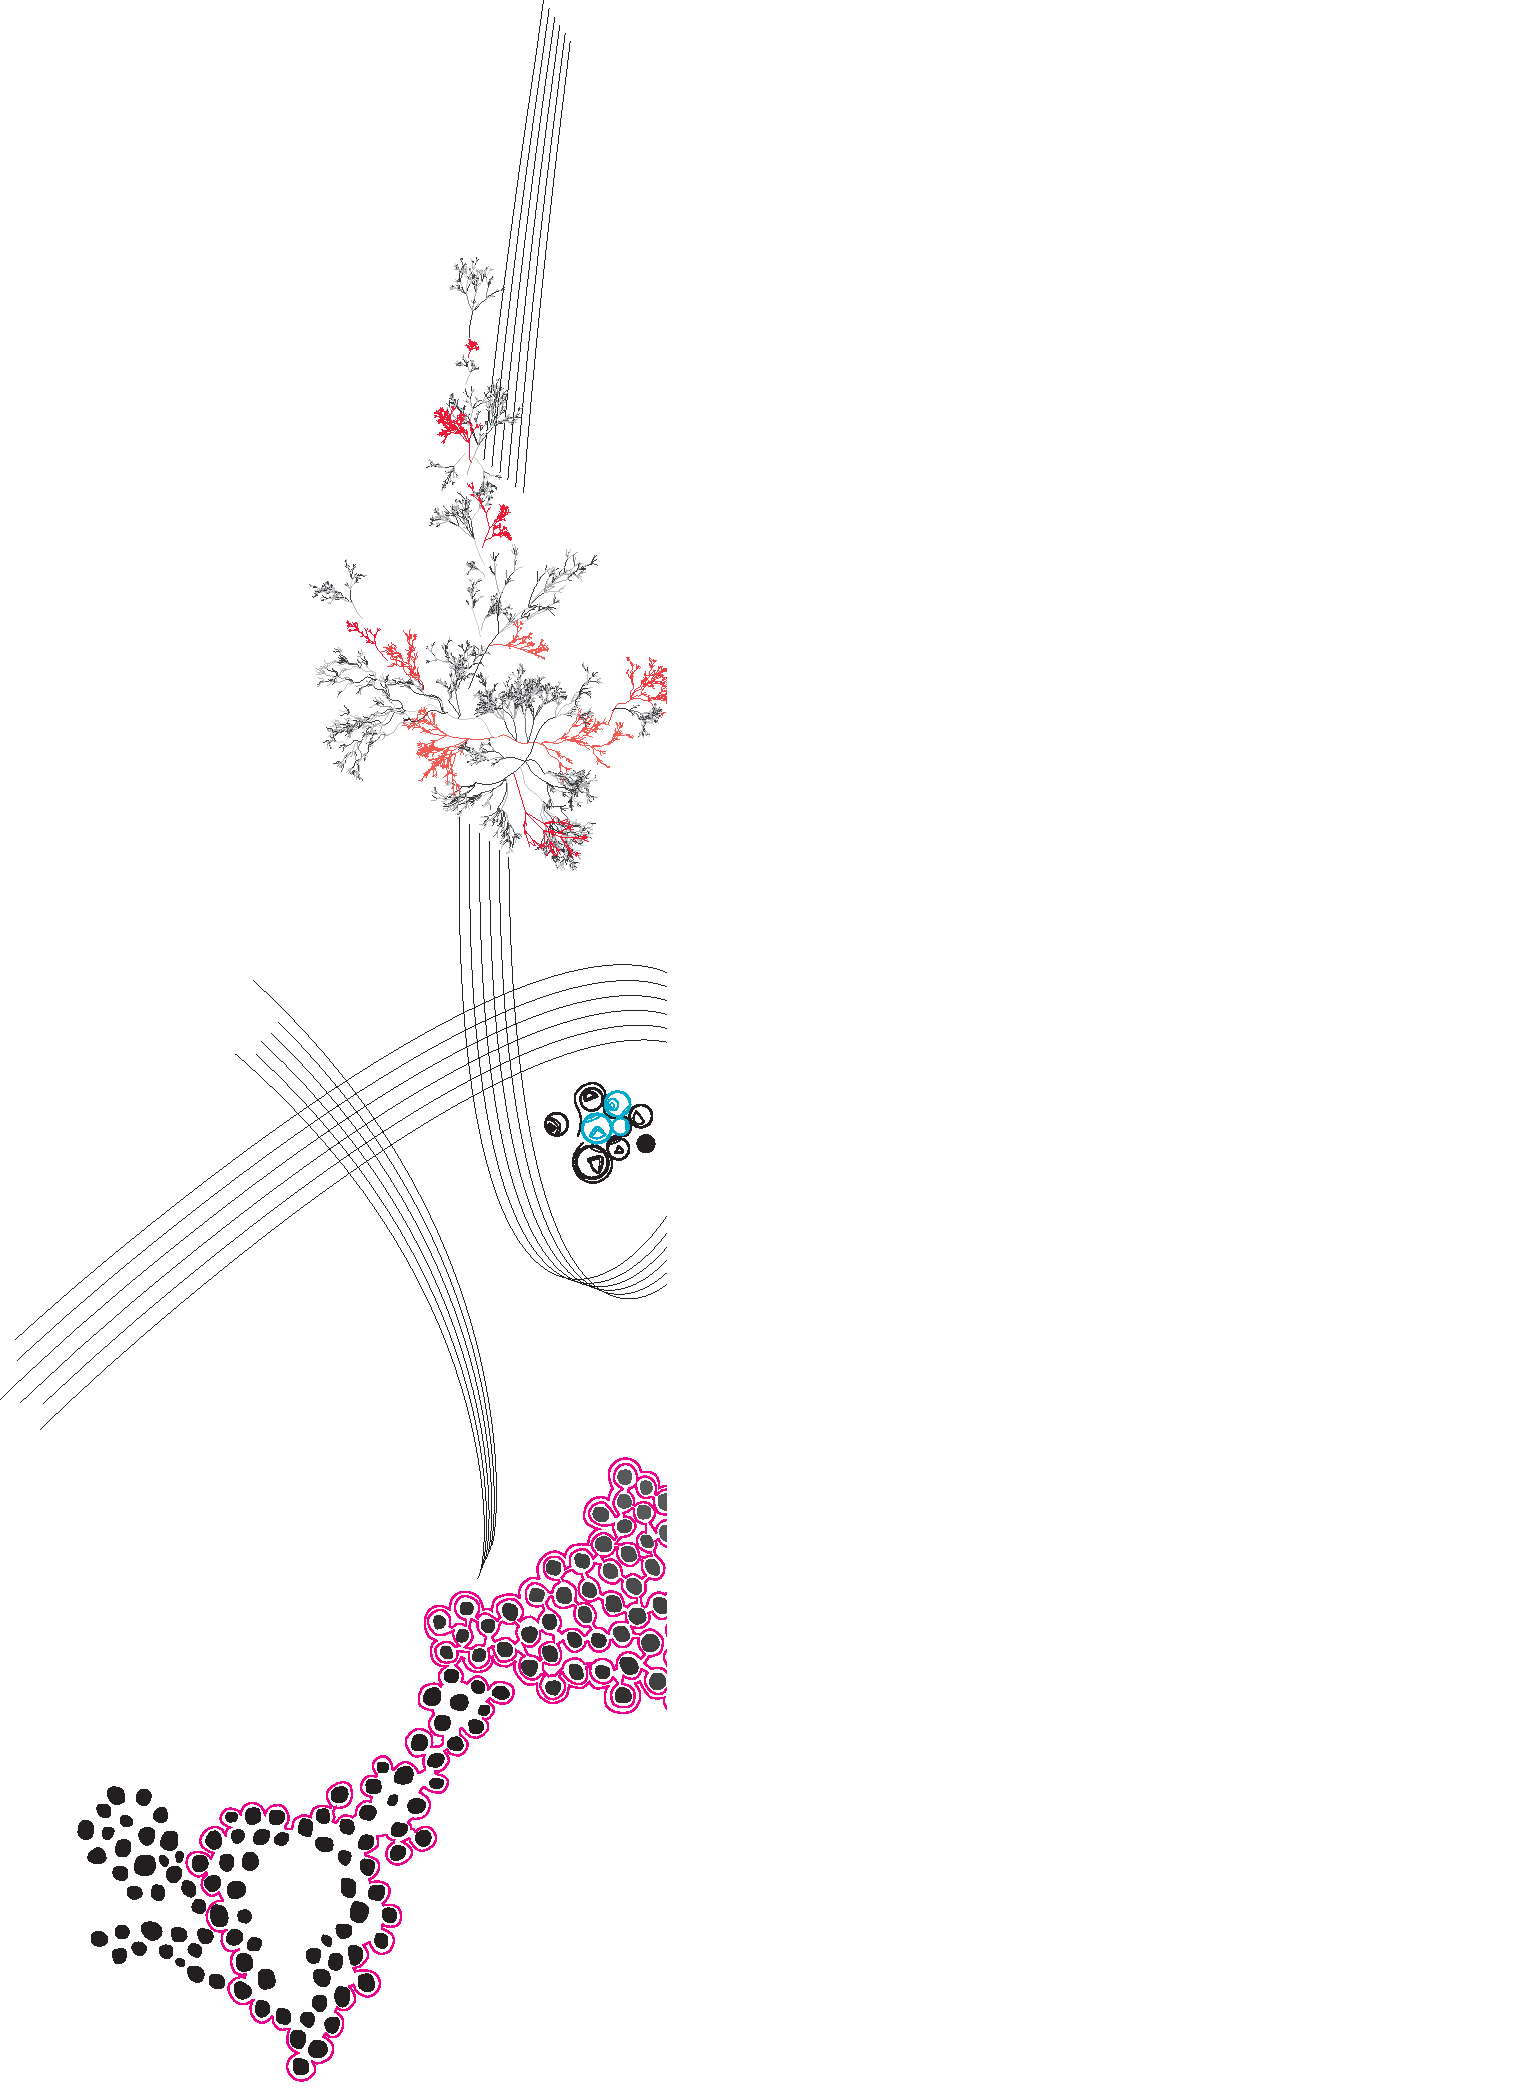
\includegraphics[width=7.5cm]{cover/utwentetitle-back-11.pdf}}%
\put(-60,-755){
\includegraphics[width=6cm]{cover/utlogo.pdf}}}
\renewcommand{\today}{\ifcase \month \or January\or February\or March\or April\or May\or June\or July\or August\or September\or October\or November\or December\fi, \number \year}
% Keywords environment (from mcs.sty)
\def\keywords{\vspace{1em}\noindent{\textit{Keywords}:\,\relax}}
\def\endkeywords{\par}
\makeatletter
\newcommand*{\coverauthor}[1]{\gdef\@coverauthor{#1}}
\newcommand*{\covertitle}[1]{\gdef\@covertitle{#1}}
\newcommand*{\doctype}[1]{\gdef\@doctype{#1}}
\newcommand*{\evalcommittee}[1]{\gdef\@evalcommittee{#1}}
\newcommand*{\makecoverpage}{%
  \thispagestyle{empty}
  \hspace{4.0cm}\parbox[t]{10.8cm}{\LARGE MSc Interaction Technology\\\@doctype}
  \vfill
  \vfill
  \hspace{4.0cm}\parbox[t]{10.8cm}{%
    \begin{flushleft}\huge{\bfseries\@covertitle}
  \end{flushleft}}
  \vfill
  \hspace{4.0cm}\parbox[t]{10.8cm}{\LARGE \@coverauthor}
  \vfill
  \hspace{4.0cm}\parbox[t]{10.8cm}{\@evalcommittee}
  \vfill
  \hspace{4.0cm}\parbox[t]{10.8cm}{\today}
  \vfill
  \hspace{4.0cm}\parbox[t]{10.8cm}{%
    Human Media Interaction\\
    Faculty of Electrical Engineering, \\
    Mathematics and Computer Science, \\
  University of Twente}%
  \newpage%
}
\makeatother
\coverauthor{Siewart van Wingerden}
\covertitle{One Thousand and One Tales \\ \small Automated Age of Empires II eSports Reports from Raw Real-time Game Data}
\doctype{Final Project}
\evalcommittee{Evaluation Committee: \\ Dr.\ Mari\"{e}t Theune \\ Dr.\ Lorenzo Gatti \\ Dr.\ Vadim Zaytsev}

% \usepackage{cite}
\usepackage{graphicx}
% used for double spacing for review
\usepackage{setspace}
\usepackage[english]{babel}
\usepackage{csquotes}
\usepackage{microtype}
\usepackage[T1]{fontenc}
% Arrays/tables helpers
\usepackage{array}
\usepackage{tabularx}
\usepackage{ragged2e}
\usepackage[sfdefault]{AlegreyaSans}
\renewcommand*\oldstylenums[1]{{\AlegreyaSansOsF #1}}

\usepackage{comment}
\setlength{\marginparwidth}{2cm}
\usepackage{todonotes}
\setuptodonotes{disable}
\usepackage{url}

% Consolidated xcolor import to prevent option clash
\usepackage[table]{xcolor}

% \usepackage[numbers,square,sort&compress]{natbib}
\usepackage[
  backend=biber,
  style=numeric-comp, % This creates [1] and compresses multiple citations to [2, 3]
  natbib=true,        % Intercepts \citet{} to print "Author [Number]"
  sorting=nyt         % Sorts the reference list alphabetically (standard for ACM/HCI)
]{biblatex}

\addbibresource{references.bib}
\setcounter{biburllcpenalty}{7000}
\setcounter{biburlucpenalty}{8000}
% Load hyperref near the end
\usepackage[hidelinks]{hyperref}
\hypersetup{
  pdftitle  = {One Thousand and One Tales: Automated Age of Empires II eSports Reports from Raw Real-time Game Data},
  pdfauthor = {Siewart van Wingerden},
  pdfkeywords = {esports; data-to-text generation; natural language generation; live commentary; Age of Empires II; large language models; user study; dataset; game telemetry}
}
\usepackage{xurl}
\definecolor{disabled}{RGB}{120, 120, 120}

\usepackage{enumitem}

\usepackage{caption}
\usepackage{booktabs}  % for nice horizontal lines
\usepackage{siunitx}   % for number alignment
\usepackage{makecell}
\usepackage{longtable} % Added for appendix tables
\usepackage{lscape}    % Added for landscape pages if needed
\usepackage{multirow}
\usepackage{threeparttable}
\usepackage{float}
\usepackage{placeins}
\usepackage{listings}

\definecolor{lightgray}{rgb}{.9,.9,.9}
\definecolor{darkgray}{rgb}{.4,.4,.4}
\definecolor{purple}{rgb}{0.65, 0.12, 0.82}

\lstdefinelanguage{JavaScript}{
  keywords={typeof, new, true, false, catch, function, return, null, catch, switch, var, if, in, while, do, else, case, break},
  keywordstyle=\color{black}\bfseries,
  ndkeywords={class, export, boolean, throw, implements, import, this},
  ndkeywordstyle=\color{darkgray}\bfseries,
  identifierstyle=\color{black},
  sensitive=false,
  comment=[l]{//},
  morecomment=[s]{/*}{*/},
  commentstyle=\color{darkgray}\ttfamily,
  stringstyle=\color{darkgray}\ttfamily,
  morestring=[b]',
  morestring=[b]"
}

\lstset{
  language=JavaScript,
  backgroundcolor=\color{lightgray},
  extendedchars=true,
  basicstyle=\footnotesize\ttfamily,
  showstringspaces=false,
  showspaces=false,
  numbers=left,
  numberstyle=\footnotesize,
  numbersep=9pt,
  tabsize=2,
  breaklines=true,
  showtabs=false,
  captionpos=b
}

% Custom column types for the coding table (inferred from appendix usage)
\newcolumntype{L}[1]{>{\raggedright\arraybackslash}p{#1}}
\newcolumntype{U}[1]{>{\raggedright\arraybackslash}p{#1}}

% Counter for appendix rows
\newcounter{AppRow}
% Spacing definitions for appendix
\newcommand{\SourceLinkGap}{0.2em}
\newcommand{\AfterSourceLinksVSpace}{0.5em}

\captionsetup{justification=raggedright,singlelinecheck=false}
% Gentle help for line breaking to reduce underfull hboxes
\setlength{\emergencystretch}{3em}
% \doublespacing

\begin{document}

\makecoverpage

\setcounter{tocdepth}{1}
\chapter*{Acknowledgements}\label{chap:personal}
This work represents the culmination of a six-year journey (enough time to be skeptical of (not so) Large Language Models and then embrace them) that would not have been possible without the support of many incredible people. While it is difficult to fully capture the depth of my gratitude in words, I want to take this opportunity to express my appreciation.

First and foremost, I would like to thank my supervisors. \textbf{Mariët}, thank you for your unwavering support and guidance throughout this process, and for the many times you went above and beyond to help me get back up and running after periods away from this research. Your encouragement, your belief in my work, and your endless ways of keeping me motivated have been a constant source of inspiration. \textbf{Lorenzo}, thank you for your insightful feedback and your invaluable technical and practical guidance, which truly shaped the direction of this project, and for finding many clever ways to motivate me and steer my creativity another way. \textbf{Vadim}, thank you for your unique perspective and for providing the critical feedback to push this work further. But perhaps the most valuable aspect of their guidance was sharing their experience as researchers; they explained to me how researchers work, what they value, and how that should be reflected in my work to ensure a meaningful and useful contribution to the field.

To my family and friends: \textbf{Mom}, \textbf{Dad}, \textbf{Sister}, and \textbf{Brother-in-law}, thank you for your unconditional love and support, especially for standing alongside me during the most challenging times. In particular, I am deeply grateful to my father, who spent many nights trying to understand the full breadth and depth of this work, and to my mother, who was never short of emotional support. Your encouragement has been a constant source of strength (and, from time to time, a healthy dose of frustration). A special thanks to my friends \textbf{Midas} (Thomas) and \textbf{Lieke} for their enthusiasm, their support, and for truly understanding my drive to see this through to the very end. I must also thank my dog, \textbf{Mara}, who was never short of enthusiasm herself, always offering the perfect support in the form of a timely walk or a cuddle.

The groundwork for this thesis was laid while I was working full-time at \textbf{CaptureAge}, which was a truly life-altering rollercoaster; an experience that led me on an unbelievable adventure alongside some of the most technically talented people I have ever had the pleasure of working with. Being able to leverage the technology we built at CaptureAge for this research has been an immense privilege. I am grateful to the company for allowing me to do so and for supporting the publication of the derived dataset. 

I also want to extend my gratitude to the competitive \textbf{Age of Empires II community}. Thank you for your enthusiastic participation in both studies, and for providing such honest and direct feedback; the only real type of feedback. May your Wololos be quick, and your villagers safe from boars.

Additionally, I would like to thank \textbf{World's Edge} for permitting the use of Age of Empires II and its recorded games, as well as the publication of the derived data. My thanks go to \textbf{MembTV} for allowing me to use his King of the Desert IV matches for the evaluation, and to \textbf{MembTV and Chris}, \textbf{T90Official}, \textbf{LidaKoR}, and \textbf{NiliAoE} for allowing me to use their shoutcasts as a data source. Finally, a special thank you to \textbf{DonDinardoni} for his invaluable help in obtaining and pre-processing the replays.
\chapter*{Abstract}

Watching electronic sports (esports) has become a mainstream spectator activity. High-quality commentary can improve the viewing experience but is resource-intensive and unevenly available across competitive matches. This thesis investigates whether high-fidelity game telemetry can be transformed into engaging live text commentary for esports spectators. Using \textit{Age of Empires II: Definitive Edition} (AoE2) as a case study, and leveraging granular match data captured via \textit{CaptureAge}, we focus on generating incremental real-time match updates that convey progression in real time.

We first conduct a domain analysis that combines prior work on shoutcasting with a preliminary study, identifying viewer-relevant content and communication strategies for real-time reporting in this domain. Based on these findings, we present \textit{SAGE} (Semantic Abstraction \& Generation from Events), a modular data-to-text pipeline that converts high-fidelity match snapshots into reportable events and generates live text commentary using Large Language Models. Two engagement-oriented modules operationalize shoutcasting-inspired strategies: \textit{Expert Insights}, which adds strategic context and clarifies the significance of key moments, and \textit{Event Structuring}, which organizes events to improve narrative flow and readability.

We evaluate the prototype with an online user study of experienced AoE2 spectators (N=33) using a within-subjects ablation design across four high-level tournament matches. Participants rate linguistic quality and engageability using measures adapted from the Motivation Scale of Esports Spectatorship. Results show that \textit{Expert Insights} improves perceptions related to competitive nature, skill improvement, and vicarious sensation. \textit{Event Structuring} improves perceived logicality but does not, by itself, increase engageability for this audience, and we find no evidence of synergistic interaction effects between modules. Participants found the texts coherent and readable while reporting limited excitement, pointing to the challenges of engaging text-only reporting and the importance of macro-level context for interpreting complex real-time strategy play.

Together, these contributions provide an end-to-end, user-evaluated account of live data-to-text generation over a dense parallel event stream and inform the design of future automated commentary systems. We also release two new datasets of continuous game-state AoE2 snapshots, 173 tournament matches and 3,100 competitive ladder matches at 1-second and 60-second snapshot resolutions. This set covers entity positions, player economy, technology state, fog of war, map layout snapshots, and layout, event and command streams.

\vfill
\begin{keywords}
  esports; data-to-text generation; natural language generation; live commentary; Age of Empires II; large language models; user study; dataset; game telemetry
\end{keywords}


\tableofcontents

\chapter{Introduction}
\label{chap:introduction}
\section{Esports, Viewers, and Game Data} 
Electronic sports (esports) have grown into a significant spectator activity. Much like traditional sports, competitively played computer games offer audiences competitive skill, strategy, and drama, broadcast on platforms such as Twitch and YouTube\cite{hamari2017, qian2020}. Both player and viewer numbers continued to rise through the early 2020s, a trend accelerated by the global pandemic, making esports financially significant for players, sponsors, and broadcasters \cite{heinrich2020, Newzoo2020}.

Viewer engagement is driven by a range of motivations: escapism, improving their own gameplay, and social interaction within the community \cite{hamari2017}. While these parallel the motivations of traditional sports spectators \cite{qian2020}, esports has one distinctive feature: it takes place entirely within a digital environment. This makes it possible to collect high-fidelity game data capturing every action and detail of game state.

However, to turn this raw data into engaging experiences that match these motivations, esports, like regular sports, relies on human commentators (shoutcasters) to guide viewers. This thesis investigates how high-fidelity game data can be harnessed to generate automated commentary that improves the spectator experience in esports.

\section{Commentary in Esports}
\subsection{Shoutcasting and the Spectator Experience}
In esports, commentary (commonly referred to as shoutcasting) is central to the watching experience. Shoutcasters provide real-time narration, analysis, and emotional depth to matches. They contextualize the action, highlight key moments, and build a narrative arc that makes the game more entertaining for the audience \cite{li2020}. Like traditional sports commentators, shoutcasters must balance play-by-play narration with strategic analysis (often referred to as color casting), often working in pairs to cover both aspects effectively \cite{kempecook2019}. While they may have access to the same video feed as viewers, their expertise allows them to interpret complex game states, predict outcomes, and explain the significance of events as they unfold.

However, high-quality shoutcasting is resource-intensive, requiring substantial preparation and in-the-moment decision making \cite{li2020}. As a result, the kinds of production support and role specialization seen at the highest levels of casting are typically concentrated in major tournaments \cite{kempecook2019}. This means expert live commentary is not available for every competitive match, leaving spectators (and players reviewing their own games) without the narrative guidance that can support the experience.

\subsection{Challenges in Automated Commentary}
The scarcity of expert live commentary for many competitive matches presents an opportunity for automated systems. The concept of automated commentary is not new; research has explored generating text from game data to improve searchability or provide basic summaries \cite{wang2021}. However, existing approaches often lack the depth and engagement factor of human commentary \cite{zhang2022, wang2021}. Claims about the benefits of such systems—such as personalization or improved viewer experience—are frequently made \cite{wang2021, zheng2025}, but rarely, if ever, supported by empirical evidence. While some work includes small user studies \cite{elarewaju2020,wang2021}, this is a critical step often overlooked \cite{vanderlee2019} across the Natural Language Generation (NLG) field.

Even the assumption that un-commentated matches would benefit from automated commentary remains underexplored. While intuition suggests that audiences could use such systems for knowledge acquisition and escapism \cite{hamari2017}, it is unclear if they can deliver on other metrics of engagement such as excitement, social interaction, or novelty \cite{qian2020}. Furthermore, even if there is interest in knowledge acquisition, it is not certain that automated commentary is the most effective delivery method, given the abundance of alternative analysis tools available to players and viewers \cite{block2018, penney2018}.

\subsubsection{From Summaries to Live Commentary}
Traditionally, automated commentary systems have focused on generating post-match summaries \cite{vanderlee2017, wiseman2017, puduppully2019}. However, to mimic human shoutcasters, this must be approached from a live commentary perspective, generating text in real time as the match unfolds. Because a system cannot summarize with information that lies in the future, commentary must be based on current and past events and generated as the match progresses. Commentary is often focused around event cues \cite{dodge2018}, which can be expressed through game data to generate live commentary \cite{taniguchi2019, wang2021, zhang2024}. This requires a different approach to data: the source must be high-fidelity enough to capture the nuances of gameplay that human shoutcasters rely on \cite{dodge2018}. This, in turn, introduces new challenges due to the complexity and volume of data involved \cite{wang2021, kim2025}.

Esports generates a sheer volume of simultaneous events \cite{lux2019}. Human casters prioritize these events for explanation \cite{dodge2018}, a skill considered vital for the viewing experience \cite{kempecook2019}. They also provide strategic insights, often preparing extensively \cite{li2020} or working in duo roles to cover both play-by-play and analysis \cite{kempecook2019}. While dashboards can assist with this \cite{charleer2018, margetis2023}, replicating this human ability to filter and contextualize real-time data remains an open challenge for automated systems \cite{dodge2018, kim2025}.

\subsubsection{Evaluation in Esports}
Evaluation in esports commentary is primarily focused on automatically calculated similarity-based metrics \cite{wang2021, zhang2022, zhang2024}. These metrics have known limitations when evaluating NLG systems \cite{vanderlee2019}, such as a limited ability to capture strategic insights \cite{wang2021}. While some efforts have been made to include human evaluation in esports commentary generation \cite{wang2024}, sample sizes are often small, do not focus on the actual target audience of esports spectators, and rely on non-standardized reporting that makes comparison across systems difficult. If the aim is to provide an experience similar to human shoutcasting of high-level matches, we believe it is essential to validate the actual utility of such systems with the target audience, especially when the goal is to improve viewer engagement or provide strategic insights.

\subsubsection{Broader Applications}
These challenges motivate the work in this thesis. By studying commentary strategies such as event prioritization and contextual enrichment, we aim to understand what automated commentary systems need to engage esports viewers effectively when consuming esports content. The problem also extends beyond esports: games offer a verifiable testbed for translating complex, parallel event streams into natural language. This is a challenge shared by sports reporting, process monitoring, and other domains where high-fidelity real-time data must be narrated for a human audience.

\section{Case Study}
In this thesis, we use live text commentary \cite{pavzanin2022, lewandowski2012} as a reporting format: short, incremental, minute-by-minute match updates provided to the reader in text as the match progresses, designed to convey progression in real-time. 

As our data source we use the real-time strategy game \textit{Age of Empires II: Definitive Edition} (AoE2) \cite{Microsoft} with competitive matches played at the highest level of its esports scene. AoE2 is an ideal testbed for several reasons:
\begin{itemize}
  \item \textbf{Strategic Depth:} It offers a deep competitive history and complex gameplay where parallel narratives unfold and meet through long-term strategy, economy management, and tactical battles.
  \item \textbf{Longevity:} With a dedicated player and viewer base for over 25 years \cite{SullyGnome}, the community has established norms and expectations for commentary.
  \item \textbf{High-Fidelity Data:} It provides a detailed real-time data source through \textit{CaptureAge} \cite{CaptureAge}, an officially supported third-party tool that streams and records detailed game data, allowing us to access the game state at a granular level. Unlike most related studies, which primarily focus on Multiplayer Online Battle Arena (MOBA) games and track only a handful of player characters, this data covers every unit, building, resource, and player action throughout the match. Unlike MOBA games where gameplay can often be summarized by linear event logs (kills, objectives), AoE2 gameplay is defined by complex economic shifts and hidden information on a procedurally generated map.
\end{itemize}

Since this research focuses on AoE2 esports and viewer motivations in a new digital domain, we will need to develop a new software system suited for its target audience. To achieve this we adopt an iterative approach, which goes through domain analysis, system design, and user evaluation phases. In practice, we followed an approach based on the Design Thinking principles \cite{brown2008}, where we first go through an inspiration phase (context and domain analysis), followed by an ideation phase (system design), and finally an implementation and evaluation phase (prototype and user study). This thesis presents a single full iteration of this process, providing the vertical slice needed to explore the research questions in depth.

This case study is also well-suited to address the gaps identified in existing esports commentary research. AoE2's rich CaptureAge data allows us to go beyond the low-fidelity event logs and video feeds that most prior systems rely on. Its established viewer community and shoutcasting culture provide the grounding needed to design engagement strategies informed by real domain expertise. And its active online community gives us direct access to the target audience for rigorous, viewer-centered evaluation. We go further into this in the next chapter (Chapter~\ref{chap:background}).

\section{Research Goals and Questions}
Building a working commentary system for one game is the immediate goal; the deeper aim is to use it as a testbed for studying what makes automated commentary engaging, with implications for real-time data-to-text generation more broadly. To this end, we adopt a "vertical slice" approach: an end-to-end pipeline for \textit{Age of Empires II} that can be refined in response to user feedback, allowing us to explore the challenges of high-fidelity data interpretation and test specific shoutcasting strategies.
\subsection{Research Goals}
To achieve these aims, we define the following research goals:
\begin{enumerate}
  \item \textbf{Interpret High-Fidelity Data:} Develop methods to translate raw, high-fidelity game data into meaningful reportable game events, capable of real-time reporting.
  \item \textbf{Apply Shoutcasting Strategies:} Identify and implement communication strategies used by human experts to keep text engaging and informative.
  \item \textbf{Generate Engaging Narratives:} Connect data interpretation with narrative generation to create text-based live text commentary, focusing on what engages viewers.
\end{enumerate}

\subsection{Research Questions}
To guide our research toward these goals, we formulate the following questions:
\begin{enumerate}[label=\textbf{RQ\arabic*:}]
  \item To what extent do commentator-inspired engagement strategies, implemented in a data-driven pipeline, improve the engageability of automated esports live text commentary?
  \item How can high-fidelity data be transformed into engaging natural language descriptions of complex esports events?
  \item How can important events in an esports match be selected and structured to form a coherent narrative?
  \item What reporting strategies are used by esports commentators and which content types do their viewers find most relevant?
\end{enumerate}

To address these questions, we proceed through the following steps, each targeting one or more RQs:
\begin{enumerate}
  \item \textbf{Domain Analysis} \textit{(RQ4):} Analyze human shoutcasting strategies and validate content relevance with viewers based on existing research and a preliminary study.
  \item \textbf{System Design \& Implementation} \textit{(RQ2, RQ3):} Translate these strategies into a system design for automated commentary and implement the designed system for live text commentary generation.
  \item \textbf{Evaluation} \textit{(RQ1):} Evaluate the system with real users to assess whether the implemented strategies improve engageability.
\end{enumerate}

RQ2 and RQ3 are design questions, answered by two architectural modules that implement commentator-inspired strategies. Their effect on engageability is evaluated as part of RQ1 through an ablation study:
\begin{enumerate}
  \item \textbf{Expert Insights:} Implements the design solution to RQ2; enriching high-fidelity data with strategic context and domain knowledge. Its effect on engageability is measured in the evaluation.
  \item \textbf{Event Structuring:} Implements the design solution to RQ3; selecting and ordering events into a coherent narrative structure. Its effect on engageability is measured in the evaluation.
  \item \textbf{Combined Effect:} Addresses RQ1 by measuring the combined and individual impact of both modules on viewer engageability.
\end{enumerate}

\section{Contributions}
This thesis makes the following contributions:

\begin{itemize}
  \item \textbf{Cross-Domain Strategy} \textit{(RQ4):} We assess prior research on shoutcasting strategies from other RTS games in the context of Age of Empires II, identifying both generalizable patterns and game-specific adaptations, and explore how these can be integrated into automated commentary systems.
  \item \textbf{The SAGE Pipeline} \textit{(RQ1, RQ2, RQ3):} We present the design and implementation of \textit{SAGE} (Semantic Abstraction \& Generation from Events), a modular data-to-text pipeline tailored for real-time esports commentary. SAGE implements the design solutions to RQ2 and RQ3 and is the testbed for evaluating RQ1. It processes high-fidelity game snapshots to detect complex events, using Large Language Models (LLMs) for NLG. To support reproducibility and future research, we release two corpora of AoE2 tournament matches (173 KotD IV matches and 3,100 matches) at 1-second and 60-second resolution, to our knowledge the largest publicly available esports game-state dataset at this resolution.
  \item \textbf{Engagement Strategies} \textit{(RQ2, RQ3):} We design and implement two commentator-inspired strategies as independently ablatable modules:
    \begin{enumerate}
      \item \textbf{Expert Insights} \textit{(RQ2):} Enriching commentary with strategic context and domain knowledge derived from high-fidelity game data.
      \item \textbf{Event Structuring} \textit{(RQ3):} Organizing events to reflect the dynamic and parallel nature of gameplay into a coherent narrative.
    \end{enumerate}
  \item \textbf{User-Centric Approach} \textit{(RQ1):} We conduct a preliminary study to identify viewer preferences and a final evaluation with the target audience to assess whether the implemented strategies improve engageability.
\end{itemize}

\section{Methodology Overview}
To address the challenges of high-fidelity data interpretation, event selection, and generating engaging real-time commentary, we adopt a user-centered design process structured as follows:

\begin{enumerate}
  \item \textbf{Context and Related Work (Chapter~\ref{chap:background}):} We define the problem space by outlining what esports commentary is and why it engages the audience, exploring the Age of Empires II domain and its high-fidelity data. We then review existing approaches in data-to-text generation and (e)sports commentary, identifying gaps in their ability to meet requirements such as narrative coherence, strategic contextualization, and appropriate evaluation methodologies.
  \item \textbf{Domain Analysis (Chapter~\ref{chap:prelim} \& Chapter~\ref{chap:viewer-study}):} Since directly relevant prior work on Age of Empires II commentary is limited, we conduct a preliminary study. We analyze professional shoutcasts to identify key event types and narrative structures, and further specify AoE2-specific requirements through a user survey.
  \item \textbf{System Design and Implementation (Chapter~\ref{chap:methods}):} Based on these findings, we design and implement a data-to-text pipeline specifically tailored for live, engaging commentary. This design prioritizes low latency and modularity to allow for the integration of engagement-focused components. We implement this design in a prototype system, \textit{SAGE}, combining a classic pipeline approach with modern Large Language Models, focusing on the technical realization of the \textit{Expert Insights} and \textit{Event Structuring} modules.
  \item \textbf{Evaluation (Chapter~\ref{chap:eval}):} Finally, since engagement is inherently subjective, we evaluate with real AoE2 viewers. We test the system's output with real AoE2 viewers to assess whether the inclusion of \textit{Expert Insights} and \textit{Event Structuring} modules leads to a more engaging experience through an ablation study. We expect each module to contribute positively to engagement.
  \item \textbf{Discussion and Conclusion (Chapter~\ref{chap:discussion}):} We interpret the results of our evaluation in the context of our research questions, discuss implications for future system design, and identify limitations. We reflect on what the findings imply for the field more broadly, including directions for further research in automated esports commentary and data-to-text generation.
\end{enumerate}
\chapter{Context and Related Work}\label{chap:background}\label{chap:related}
Automated commentary sits at the intersection of esports broadcasting, game-domain structure, and high-fidelity telemetry. This chapter introduces (1) live text commentary, (2) esports spectatorship and shoutcasting roles, (3) \textit{Age of Empires II} (AoE2) as the target domain, and (4) the game data surfaced through \textit{CaptureAge}. It then reviews related work in data-to-text Natural Language Generation (NLG) and (e)sports reporting, including work on summarization, engagement, and evaluation, and identifies gaps that motivate our approach.

Because directly relevant prior work is limited, we draw on esports studies and adjacent research to provide theoretical grounding. Where helpful, we also draw on the author's professional experience as a lead designer and developer at CaptureAge and in AoE2 to contextualize design decisions made throughout the project.

\section{Live text commentary}
\label{sec:live-text-commentary}
Live text commentary, also discussed as Online Sports Commentary (OSC), is a reporting genre of short, incremental textual updates during a match \cite{pavzanin2022, lewandowski2012}. Unlike spoken shoutcasting, which relies on engaging speech and visual cues, live text updates emphasize concise content selection and summarization. For this thesis, we adopt this format to isolate the core challenges of content selection and narrative generation from real-time audio synthesis, which can be addressed in future work.

OSC is designed to inform readers about ongoing action via minute-by-minute updates and commonly uses present tense forms to create the impression that events are unfolding in real time \cite{lewandowski2012}. \citet{lewandowski2012} provides the following example from a soccer match live text commentary:

\begin{quote}\itshape
  116’ GOAL! GOAL! INIESTA PUTS SPAIN INTO THE LEAD AND ON THE VERGE OF WORLD CUP GLORY! Iniesta is played in by Fabregas and the Barcelona man finishes brilliantly!
\end{quote}

While not the same as live spoken commentary, it still shares many of the paralinguistic features of live commentary, such as the use of present tense, temporal anchoring, and an overall style that aims to maintain excitement \cite{lewandowski2012}. It also uses genre conventions such as informal vocabulary, metaphors, and occasional questions to build a more personal relationship with readers \cite{lewandowski2012,pavzanin2022}.

\section{Esports}
\subsection{Defining Esports}
The esports industry spans genres including real-time strategy (RTS; Age of Empires), first-person shooters (FPS; CounterStrike), multiplayer online battle arenas (MOBA; League of Legends, DotA2), and fighting games (Super Smash Bros.) \cite{reitman2020}. Viewers tune in for entertainment, social interaction, and learning game strategies and mechanics \cite{sjoblom2017}.

\citet{cranmer2021} offer definitions of esports ranging from professional competitive gaming to broader interpretations. For this thesis, we adopt a broad definition that includes the "traditional (multi-player) game experience" and "Competitive Multiplayer Computer Games," aligning with \citet{hamari2017}: esports is "a form of sports where the primary aspects of the sport are facilitated by electronic systems; the input of players and teams as well as the output of the esports system are mediated by human-computer interfaces." This definition highlights a core difference from traditional sports: the digital substrate. Every player action and its outcome is routed through a computer system governed by game rules, enabling high-fidelity data collection. This data is commonly used for dashboards and overlays, but less often for narrative generation.

\subsection{Shoutcasters}
Raw gameplay alone is often insufficient to fully engage an audience. Just as football relies on commentators to explain the offside rule or build anticipation for a penalty kick, esports relies on \textit{shoutcasters} to build a narrative around the action \cite{kempecook2019}. These broadcasts, often streamed to large audiences on platforms such as Twitch and YouTube, transform a series of game states into a coherent story.
Shoutcasters (or commentators) are essential for generating excitement and providing context. They typically fall into two archetypes and often operate as a duo, though they can switch between these roles fluidly \cite{li2020} or operate solo \cite{kempecook2019}:
\begin{itemize}
  \item \textbf{Play-by-Play Caster:} The enthusiastic narrator who describes the immediate action (the \textit{what}). Their fast-paced delivery mirrors the intensity of a battle, building suspense and emotional release. They use different techniques both linguistically \cite{byro2017,gustin2020} and structurally \cite{penney2021, cheung2011starcraft} to maintain viewer engagement.
  \item \textbf{Color Caster:} The analyst who explains the strategic context (the \textit{why}). They focus on explaining motivations and strategies, filling lulls with insightful commentary and providing entertainment value \cite{li2020}.
\end{itemize}
This parallels traditional sports commentary, where a play-by-play announcer describes the action and a color commentator provides analysis and background (e.g., team rivalries) \cite{bryant1982}. In this thesis, we use these roles to inform system design: we do not aim to replicate a human shoutcaster's energetic delivery in live text updates, but we do aim for informative, engaging reporting grounded in objective data, since shoutcasting corpora often embed personalized experiential knowledge that an automated system cannot authentically replicate.

\subsection{Viewers}
Esports titles are visually complex and rule-dense, with many simultaneous attention points \cite{lux2019}. Without a guide, this complexity can be overwhelming. The caster's job is to filter and prioritize, directing attention to critical moments \cite{kempecook2019}. In RTS titles, the multiplicity of attention points also challenges the players themselves and transfers to the audience. Viewers are engaged by different shoutcasting strategies \cite{cheung2011starcraft,block2018},

Esports viewing is often communal, with audiences gathering in physical or online communities \cite{sjoblom2017}. Casters link game and audience, building community through shared excitement and analysis.

\subsection{Engagement Factors}
Beyond role and structure we look at engagement. \citet{cheung2011starcraft} suggests that Information Asymmetry (telling the viewer something the player doesn't know) is a key driver of engagement. \citet{block2018} found that showing context-relevant historical data elicits emotional responses, and that viewer-facing graphical content in DotA2 supports storytelling and viewer engagement. This suggests that effective automated commentary should explain the strategic significance of events (e.g., what a Castle being built implies about the opponent's next move) rather than simply reporting game actions.

\subsection{Linguistic Patterns}
Linguistic patterns in esports and live text commentary have not been extensively studied, but comparative work can inform what automated systems should produce. \citet{byro2017} found that professional casters use more complex sentence structures, extreme adjectives, and figurative language to build hype, whereas non-professional casters more often use simpler constructs (e.g., \textit{intensifying adverb + positive adjective}). \citet{gustin2020} found that promotional esports language in Super Smash Brothers: Melee uses similar constructs to Mixed Martial Arts, differing mainly in domain-dependent vocabulary. \citet{lewandowski2012} contrasted live summarization (Online Sports Commentary), live commentary (Sports Announcer Talk), and post-hoc summarization (Written Sports Commentary), identifying simple present tense and ellipsis (subject and copula deletion) as key features for live summarization; \citet{pavzanin2022} similarly found that text updates often mimic paralinguistic patterns of live commentary to convey excitement. These patterns (active verbs, specific terminology, and narrative transitions) distinguish engaging commentary from rigid templates, and inform what automated systems should aspire to while respecting that live commentary and live summarization differ.

\subsection{Spectatorship Motivations}
\label{sec:mses-motivations}
Esports spectatorship motivations have been studied through established instruments such as the Motivation Scale for Sport Consumption (MSSC) \cite{trail2001,hamari2017,sjoblom2018} and Uses and Gratifications Theory \cite{katz1973,sjoblom2017}. However, these frameworks do not fully capture the interactive and immersive nature of esports. \citet{qian2020} addressed this by adapting MSSC into the Motivation Scale of Esports Spectatorship (MSES), identifying ten motivations specific to esports viewing; we summarize them as follows:
\begin{itemize}
  \item \textbf{Skill Improvement:} Watching to learn new strategies and improve one's own gameplay.
  \item \textbf{Skill Appreciation:} Admiring exceptional skills and unique plays by professionals.
  \item \textbf{Vicarious Sensation:} The feeling of being "in the game" and experiencing it through the player.
  \item \textbf{Competition Excitement:} The thrill and arousal derived from the competitive atmosphere.
  \item \textbf{Friends Bonding:} Strengthening real-world friendships through shared viewing experiences.
  \item \textbf{Socialization Opportunity:} Interacting with the broader online community and streamers.
  \item \textbf{Dramatic Nature:} The appeal of uncertainty, comebacks, and underdog stories.
  \item \textbf{Entertaining Nature:} Seeking fun and pleasure from the content.
  \item \textbf{Competitive Nature:} The enjoyment of high-level competition and rivalry.
  \item \textbf{Game Knowledge:} Interest driven by a deep understanding of the game's mechanics.
\end{itemize}

We use these motivations as a lens for \textit{engageability}: we posit that engageability of an esports commentary system can be measured by how well it serves spectatorship motivations. Our automated commentary system is well-positioned to support \textit{Skill Appreciation} and \textit{Game Knowledge} by surfacing match and external data. Narrative structuring may also help foreground \textit{Dramatic Nature} and \textit{Competition Excitement} by highlighting turning points and narrative arcs. However, social motivations such as \textit{Friends Bonding} and \textit{Socialization Opportunity} are difficult for a text-based automated system to replicate, as they rely on human-to-human interaction and communal viewing.

\section{Age of Empires II}
To test our theories, we need a domain that offers both strategic depth and narrative richness. For over two decades, \textit{Age of Empires II} (AoE2) has challenged players to guide a civilization from the "Dark Age" to the "Imperial Age," balancing a fragile economy with the need for military conquest: aiming to disrupt the opponent's economy.

The game emphasizes hidden information through two key elements: the "Fog of War," which obscures enemy actions, and a randomly generated world map. This requires players to use their scouts to actively explore the map. For instance, spotting an opponent's Stable might trigger the training of Pikemen to counter any cavalry that is likely to appear, while discovering an expansion to Gold Mines might require pressuring that resource or preparing to counter Archers (which require gold to produce). These interactions create an evolving narrative of scouting, adaptation, and execution.

To visualize the game mechanics, Figure~\ref{img:aoe2gameplay} provides an annotated screenshot of an early-game AoE2 match, highlighting key interface elements, resource nodes, buildings, and units.

\begin{figure}[h]
  \centering
  \includegraphics[width=\textwidth]{assets/AoE2-Explanation.png}
  \caption{The player's perspective in Age of Empires II: An overview of the early game showing economy management, unit production, and exploration.}
  \label{img:aoe2gameplay}
\end{figure}

\begin{enumerate}[leftmargin=*,noitemsep,topsep=0pt]
  \item \textbf{Interface Elements:} The interface includes resource stockpiles, population, the current Age, and queued units and technologies (not shown), supporting decision-making.
  \item \textbf{Resource Nodes:} Examples include Gold Mines, Stone Mines, and Farms. These nodes fuel the economy that supports expansion and military production.
  \item \textbf{Town Center:} Produces Villagers and serves as an early drop-off and defense point. Building additional Town Centers is expensive but increases Villager production. It also enables advancing to the next Age, which temporarily halts Villager production but unlocks new buildings, units, and technologies. Key skills include deciding when to add Town Centers or advance ages, and maintaining Villager production with minimal idle time.
  \item \textbf{Blacksmith:} A key military building for researching upgrades (e.g., armor and attack enhancements) that shape unit effectiveness.
  \item \textbf{Barracks:} The first military building available, enabling early infantry and unlocking more advanced military buildings.
  \item \textbf{Economic Buildings:} Structures such as the Mill and Mining Camp act as drop-off points and unlock upgrades that improve resource gathering rates.
  \item \textbf{Villagers:} The primary economic unit responsible for gathering resources, constructing, and repairing buildings; they may also be used aggressively to claim land and resources.
  \item \textbf{Houses:} Increase the population limit, allowing players to train more units; early on, Houses are also used to block enemy units.
  \item \textbf{Scout Cavalry:} The initial scouting unit used to explore the map, uncover the Fog of War, and locate resources and enemy positions.
  \item \textbf{Fog of War:} Black areas are unexplored, while gray areas have been seen but are not currently visible (showing the last known state instead).
  \item \textbf{Score Panel:} Provides a quick, high-level summary of each player's performance.
  \item \textbf{Minimap:} Provides a strategic overview of the battlefield and Fog of War and allows for quick navigation of the main view.
\end{enumerate}

\subsection{Competitive Play}
Competitive AoE2 is often described in phases. It begins with the \textit{Dark Age}, a period of precise, optimized \textit{build orders} where seconds matter, while following well-laid-out steps to set up the initial strategy. Then players can choose to transition into the \textit{Feudal} and \textit{Castle} ages, where this initial strategy branches and the first skirmishes occur. Finally, it culminates in the \textit{Imperial Age}, a chaotic clash of massive technologically advanced armies and siege engines or booming economies. Sometimes, as the world's resources dwindle, players resort to massive armies of cheap units, hoping to edge out their opponent through larger stockpiles and clever pressure points.

This variable pacing is a key challenge for summarization. A system must be versatile enough to explain the subtle economic maneuvering of the early game and the frantic, multi-front warfare of the late game without losing the narrative thread. All while ensuring that the state of technologies and the economy is accurately updated.

\subsection{CaptureAge \& Game Data}
AoE2 has a long-running, community-driven competitive scene with a knowledgeable audience. Viewers appreciate clever strategies such as hidden tech switches and economic booms, and casters interact with viewers in real-time through platforms like Twitch. From this community emerged CaptureAge, a widely used analysis tool that, for this thesis, provides access to a highly granular view of game state.

Unlike traditional sports analytics, which often rely on computer vision to estimate positions, CaptureAge hooks directly into the game engine, live-extracting actions, state changes, and events in real time. This enables a full rerender of the match and supports live and post-match statistics and analysis. The data is granular and structured.
This richness is our greatest asset and our biggest challenge. Unlike computer vision approaches where events must be inferred, CaptureAge records engine-state data directly. The challenge lies in \textit{connectedness}: determining causal links between seemingly isolated events; on a simple level (e.g., which damage events belong to the same battle) but also more complicated (e.g., how a villager loss in the early game leads to a resource deficit and subsequent military defeat).

\section{Other Game Data Sources}

Structured esports datasets fall broadly into \textit{event logs} (discrete timestamped transitions such as kills, unit production, or research completions) and \textit{continuous state snapshots} (a record a full cross-section of the game world at regular intervals). Continuous snapshots are substantially rarer, and the publicly available examples tend to come from games with a compact state space.

For FPS titles, ESTA~\cite{xenopoulos2022} provides CS:GO professional matches as pre-exported JSON at 2 Hz, covering player positions, health, cash, and action events; CSKnow~\cite{durst2022} offers a similar export at 1 Hz. These are the clearest examples of continuous, downloadable game-state snapshots in esports research. For MOBAs, a large community dataset of League of Legends decoded replay packets~\cite{maknee2024} covers over 700,000 matches with positions and unit states, but is event-driven rather than continuously sampled, impacting how the data can be utilized; OpenDota~\cite{opendota} covers Dota\,2 at post-match statistics level only.

RTS titles present a more complex space. The state space is far larger with hundreds of individually addressable entities, per-player economy, technology research trees, and command queues. No publicly available dataset combines all of these in a continuous snapshot format. SC2EGSet~\cite{sc2egset2023} is the largest structured StarCraft II dataset (17,930 tournament replays, pre-exported JSON on Zenodo), but explicitly excludes unit positions, which cannot be extracted without the game engine. StarData~\cite{synnaeve2017} exports Brood War full play command and game data at a high frequency; however, this dataset is no longer publicly available, and would need to be re-processed. For AoE2 specifically, the OCEL 2.0 dataset~\cite{aoe2ocel2024} provides event logs for 100,000 matches (commands, production, research), and a smaller export~\cite{aoerecinfo} covers 100 matches at 20-second resolution with resource counts and positions but no game state data. Beyond datasets, APIs exist for DotA2~\cite{valve,barot2017}, League of Legends~\cite{riotgames}, and StarCraft II~\cite{blizzard}, but are oriented toward bot development or post-match statistics rather than full state export.

StarCraft II, which is mechanically closely related to AoE2, has also been a main focus for shoutcasting research \cite{penney2021,cheung2011starcraft}, motivating the cross-domain analysis in Chapter~\ref{chap:prelim}. AoE2's active modding community, CaptureAge's data completeness, and its intuitive mechanics, which make generated narratives accessible outside the core player base, motivate it as our target domain \cite{CaptureAge}.

\section{Data-to-Text Generation}
Data-to-Text (D2T) generation transforms structured data into natural language \cite{gatt2018}. In our setting, it bridges game data and audience-facing commentary. D2T spans domains from weather and health to sports \cite{ramos2019,pauws2019,vanderlee2017}. We focus on D2T approaches most relevant to esports reporting: modular pipelines, end-to-end statistical models, and hybrid approaches.

Classic approaches, exemplified by \citet{reiter2000} and BabyTalk \cite{reiter2007}, decompose generation into staged pipelines (Signal Analysis \(\rightarrow\) Data Interpretation \(\rightarrow\) Document Planning \(\rightarrow\) Realization), as depicted in Figure~\ref{fig:pipeline-reiter}. Their strength is controllability: reporting decisions can be constrained and explained, which is essential in domains like healthcare and is also relevant for esports reporting where learning is a core viewer motivation \cite{reitman2020}. More recent work emphasizes end-to-end statistical (often neural) models \cite{gatt2018}, which produce more fluent text but are harder to constrain and can hallucinate facts. This is a critical flaw when trying to explain a complex game state accurately \cite{wang2019}.

\begin{figure}[htbp]
  \centering
  \IfFileExists{assets/pipeline-reiter.pdf}{%
    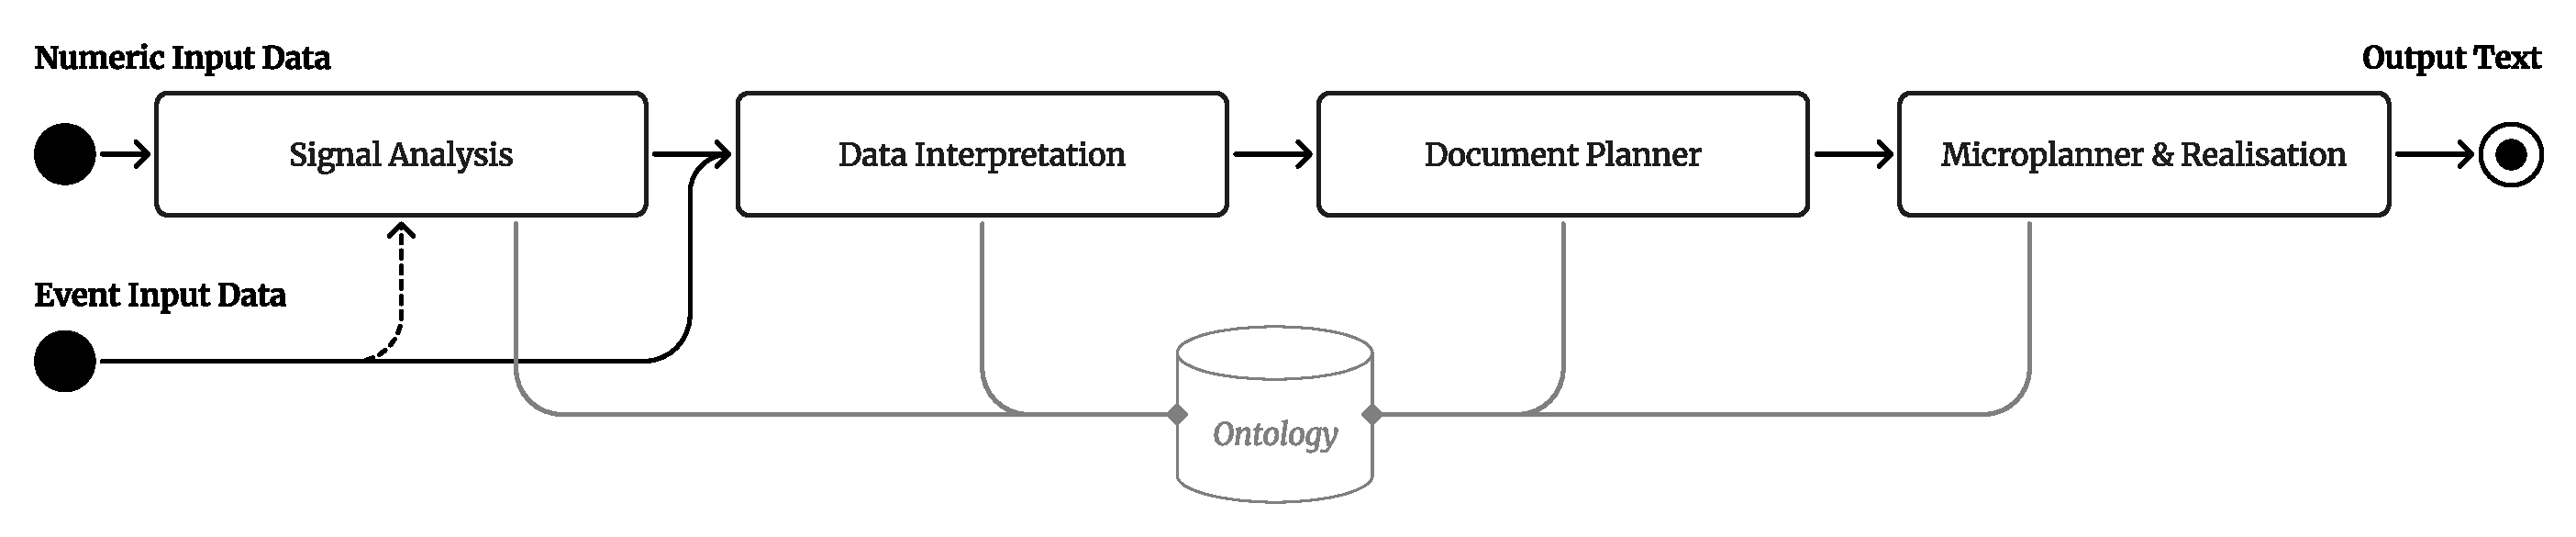
\includegraphics[width=\textwidth]{assets/pipeline-reiter.pdf}%
  }{%
    \fbox{\parbox{0.95\textwidth}{\centering Placeholder: missing file\\`assets/pipeline-reiter.pdf`}}%
  }
  \caption{The classic BabyTalk pipeline as proposed by \citet{reiter2007}. Continuous numeric data enters \textit{Signal Analysis}, while symbolic event data enters \textit{Data Interpretation}. Event data also supports Signal Analysis for pattern detection \cite{portet2008}.}
  \label{fig:pipeline-reiter}
\end{figure}

A critical challenge in D2T is bridging low-level data streams and high-level narrative events. Even statistical models often rely on intermediate structured representations \cite{chiang2025}; low-level data needs to be abstracted into reportable events via Signal Analysis \cite{portet2008}. Prior work spans rule-based detection, fuzzy logic \cite{ramos2019}, machine learning \cite{zhang2024}, and process mining \cite{zelst2021}. Within gaming, AlphaStar's StarCraft II work illustrates how rich game-state representations can capture complex dynamics \cite{mathieu2023}, even when summarization is not the primary goal.

\section{Sports and Game Commentary Generation}
Commentary generation for sports and games is a long-standing application of data-to-text systems, partly because outputs can often be checked against underlying data. We highlight work in both traditional sports and computer games that is relevant to esports commentary.

\subsection{Traditional Sports and Board Games}
Traditional sports and board games have provided benchmarks for post-game reporting and live commentary, supported by structured event logs and stable reporting conventions. This includes datasets like RotoWire \cite{wiseman2017} and reporting systems like PASS \cite{vanderlee2017}.

Work on live commentary spans early template systems such as ROCCO for RoboCup \cite{voelz1998} and neural models over event streams for soccer \cite{taniguchi2019}. Board-game commentary has also been explored in domains like chess \cite{zheng2025}, where the data volume differs substantially from esports.

Recent work increasingly uses LLMs downstream of event detection, for example from video \cite{andrews2024} or from match data \cite{cook2024}. Other systems emphasize retrieval or external knowledge for contextual depth (SCoReS \cite{lee2013}; Wikidata-enhanced PASS \cite{gatti2018}). These efforts motivate grounded realization, confirming that our setting must abstract higher-volume game-state data into reportable events.

\subsection{Esports Commentary}
Earlier game commentary work focused on \textit{Let's Play} content, informal first-person playthroughs targeting entertainment rather than competitive analysis, and reports substantial room for improvement in contextual relevance \cite{guzdial2018,shah2019,li2019}. Esports commentary is more demanding: it must convey strategic depth to a knowledgeable audience in real time. We review the most relevant work below.

Bardic \cite{barot2017} uses high-fidelity DotA2 data to generate world renders and text output, inferring player intentions by tracking actions over time windows and expressing them through hand-implemented story schemas.

\citet{elarewaju2020} used Probabilistic Lexicalized Tree-Adjoining Grammars (TAGs) trained on annotated caster data to generate text for esports highlights. The rule-based approach produced accurate event descriptions, though output quality was perceived as higher when paired with audiovisual content.

The work of \citet{wang2021} is closest to our setting, generating natural language commentary for League of Legends esports. They pair game-event data with commentary transcripts and train neural sequence models with hierarchical encoding, a technique that groups fine-grained game events into higher-level structures so they can be expressed as coherent sentences rather than fragmented lists. However, no viewer evaluation was reported in that work; \citet{wang2024} later conducted one at limited scale in follow-up research. A key limitation of the end-to-end framing is reduced control over content selection, which can cause misalignment between game events and generated text. \citet{wang2024} extend the approach with LLMs, finding Llama2-13B performs best on automatic metrics, but the core problem persists: the system still struggles to associate past game events with the current context, confirming that end-to-end framing alone is insufficient for coherent commentary. Together, these results motivate LLM-based realization paired with explicit upstream abstraction of game state.

\citet{zhang2022} compare rule-based and LLM-based realization for DotA2 event commentary, finding LLM realization outperforms rule-based on automated metrics, supporting the hybrid pipeline direction. \citet{zhang2024} take a different approach: rather than structured game data alone, they introduce GAME-MUG, a multimodal dataset for League of Legends commentary that combines game event logs, caster speech audio, and audience chat. They propose a joint multimodal dual learning model for game situation understanding and commentary generation. While our setting is text-only and structured-data-driven, their work highlights the potential of richer input modalities and audience-side signals for improving commentary quality.

\section{Summarization}
Selecting the most relevant events from a continuous stream and presenting them coherently is a challenge shared by live commentary generation and summarization alike. Reducing the amount of information for textual formats is something we have already mentioned for traditional sports as "OSC" \cite{lewandowski2012}. In esports, summarization and highlights are often regarded as the same, both identifying exciting moments, while true summarization also requires narrative coherence and explanatory context. Highlights can still provide a good baseline for narrative summarization, as they represent moments of the game worth highlighting.

\subsection{Highlight Detection}
Most existing work in esports highlight detection focuses on finding the ``best'' moments from audiovisual signals, rather than generating explanatory commentary. \citet{chu2017} reviewed computer-vision methods using visual features (e.g., motion intensity) and psycho-physiological proxies (e.g., chat/emotes). \citet{song2016} used Convolutional Neural Networks on visual features, and \citet{ringer2018} analyzed voice volume and facial expressions.

None of these methods use structured game data, relying instead on video and audio analysis. They identify exciting moments but do not explain why those moments matter, a gap that commentary generation can fill. We can learn from such systems by understanding if features like motion intensity are also captured in structured game data (e.g., unit production, battles).

\subsection{Narrative Summarization}
True summarization requires understanding causal links between events. The GameStory task \cite{lux2018, lux2019a, ninh2018, wutti2018} targeted this for CounterStrike, aiming to "boil down a long game to its most important events." Many submissions relied on heuristics (e.g., round start, bomb plant) and struggled to produce a cohesive story, showing that filtering alone is not enough for engaging, informative summaries.

To better use Large Language Models (LLMs) for reporting in games, \citet{kim2025} compress low-level game data into higher-level filtered representations to fit within a reduced context window. They evaluate analytical accuracy and identification of pivotal events, using heuristics (e.g., momentum changes based on win probabilities) to select important moments. This work is closely related, although summarization is treated primarily as a technical requirement for LLM use.

The gap lies in constructing narratives that go beyond event detection to explain the \textit{why} behind events.

\subsection{Event Relevance in Esports}
Selecting the right events is only part of the problem; summaries also require supportive information that explains \textit{why} an event matters in context. Research on supporting information in esports spectating shows that context matters: the right information must be shown at the right time \cite{charleer2018} (e.g., performance measures during a battle). However, little work directly addresses what is relevant for summaries in Age of Empires II (AoE2). Adjacent analyses, such as \citet{penney2021} on StarCraft II, identify described event types and supportive information. We will investigate these more in Chapter~\ref{chap:prelim} and Chapter~\ref{chap:viewer-study}.

\section{Evaluation of NLG Systems}
Evaluating the quality of generated text is a longstanding challenge in NLG. While standard automated metrics are widely used for benchmarking, they often fail to capture the nuances of narrative quality and reader engagement, which are central to this thesis.

\subsection{Automated Metrics}
The most common evaluation methods in NLG are n-gram overlap metrics such as BLEU \cite{papineni2002}, ROUGE \cite{lin2004}, and METEOR \cite{banerjee2005}. These metrics calculate a score based on the lexical similarity between the generated text and one or more human-written reference texts. While they are useful for tracking system improvements in tasks like machine translation, they have been shown to correlate poorly with human judgments of quality in open-ended generation tasks \cite{reiter2018,vanderlee2019,vanderlee2021}.

For creative domains like sports commentary, where there are many valid ways to describe the same event, these metrics are particularly limited. They cannot assess whether a narrative is exciting or insightful, only whether it uses the same words as the reference. Furthermore, they fail to measure factual correctness, a critical requirement for our system. As \citet{wang2021} noted in their work on esports commentary generation, standard metrics are unable to capture game-level strategic insights, which are essential for engaging commentary.

\subsection{Human Evaluation}
Given the limitations of automated metrics, human evaluation remains the gold standard for assessing NLG systems, but depends on the specific aims of the text \cite{vanderlee2019}. Human evaluation typically involves asking participants to rate generated texts on Likert scales. Automated metrics can be useful in constrained, reference-based tasks, but they struggle to assess \textit{Informativeness} (Does the text convey the necessary information?) and \textit{Enjoyment} (Is the text interesting and enjoyable to read?).

\noindent \Citet{vanderlee2019} emphasize the importance of using appropriate participant pools and clearly defined criteria to ensure reliability. In the context of esports, this means involving participants who are familiar with the game mechanics and terminology, as general readers may not be able to judge the accuracy or insightfulness of the commentary.

\subsection{Participant Recruitment for Esports Studies}
Recruiting participants familiar with the game is a real constraint when evaluating esports commentary systems. \citet{lux2019a} used professional game analyzers to verify summary quality; esports-related subreddits have also been shown to contribute substantial questionnaire respondents \cite{hamari2017} (In particular during the pandemic, when this research started.), with prior AoE2 questionnaires confirming this as an active channel for reaching the player and viewer community \cite{bidermayer2020}.

\subsection{Architectural Evaluation}
Beyond evaluating the final output, it is often necessary to assess the contribution of individual system components. \citet{callaway2002} proposed an architectural ablation approach for evaluating narrative generation systems. By systematically enabling and disabling specific modules (e.g., narrative planning, lexical choice), researchers can measure the impact of each component on the overall quality. This glass-box evaluation matters most for complex pipelines, where errors propagate from one stage to the next.

\section{Discussion and Gap Analysis}
The existing literature covers the components we need — modular pipelines, neural generation models, and linguistic work on what keeps audiences engaged — but a gap remains:
In the esports commentary systems we reviewed, many either rely on low-fidelity data (video pixels) or produce low-fidelity output (simple templates). Few have attempted to harness deep, structured game-state data (such as the data provided by CaptureAge) to generate high-level, strategic narratives.

Rule-based and hybrid data-to-text approaches can provide control over what is said and how it is expressed without requiring large amounts of annotated training data. We build on this by employing linguistic techniques and surfacing data that emphasizes information asymmetry between spectator and player.

Prior esports commentary systems primarily use event logs or metadata \cite{wang2021, wang2024, wang2025, barot2017, elarewaju2020, zhang2022} or multimodal broadcast cues \cite{zhang2024}; work using complete game-state data, like AlphaStar \cite{mathieu2023}, targets player AI rather than reporting. Across these directions, rigorous viewer-centered evaluation is rare, systems are often assessed via technical proxies rather than what viewers actually find useful, and it remains unclear how to turn high-fidelity game-state telemetry into efficient, state-aware strategic narratives grounded in esports communication research.

This thesis addresses these gaps in three concrete ways. First, we ground content selection and engagement strategies in a qualitative domain analysis of professional shoutcasting, informed by esports media studies (Chapter~\ref{chap:prelim}) and a preliminary viewer study (Chapter~\ref{chap:viewer-study}). Second, we use CaptureAge's high-fidelity game-state data to generate strategic narratives that go beyond what surface-level event logs or video can support (Chapter~\ref{chap:methods}). Third, we evaluate directly with the AoE2 viewer community using engagement-oriented measures derived from esports spectatorship research, rather than relying on automated proxy metrics (Chapter~\ref{chap:eval}).
\chapter{Domain Analysis}\label{chap:prelim}
To decide what to include in narrative summaries, we analyze professional Age of Empires II (AoE2) commentary using a cross-domain lens. StarCraft II (SC2) shoutcasting work \cite{dodge2018, penney2018, penney2021}\footnote{\citet{penney2021} supersedes the earlier two papers \cite{dodge2018, penney2018}; however most of our analysis predates it. We refer to \citet{penney2021} for the most detailed findings, but otherwise cite the earlier two.} provides a reusable account of what shoutcasters say and which information they draw on. Because SC2 and AoE2 are both real-time strategy (RTS) games yet differ in pace and mechanics, we examine which findings transfer to AoE2. This analysis addresses RQ4 from Chapter~\ref{chap:introduction}, explaining what reporting strategies commentators use and how these align with viewer engagement through the following sub-questions:
\begin{enumerate}[noitemsep, topsep=0pt]
  \item \textbf{RQA1:} How similar is AoE2 to StarCraft II in terms of information and commentary strategies?
  \item \textbf{RQA2:} What information and knowledge are used to commentate on match events?
  \item \textbf{RQA3:} What narrative structure is used to report on a competitive AoE2 match?
\end{enumerate}
Which content types AoE2-specific viewers actually value is validated in the preliminary viewer study (Chapter~\ref{chap:viewer-study}).

\section{Methodology}
For this we adapt the SC2 analysis approach used by \citet{dodge2018, penney2018} to AoE2 using three lenses: (1) PEAS + Information Foraging Theory (IFT) for cue-driven information access \cite{russell1995, pirolli1999}, (2) intelligibility types \cite{lim2009} for the implicit questions answered, and (3) utterance-level coding inspired by linguistic coding work \cite{metoyer2010}. Based on our findings we motivate the design of the viewer study and yield design implications for our system.

\subsection{Information Foraging \& PEAS}
Information Foraging Theory (IFT) \cite{pirolli1999} describes the location (\textit{patches}), order and routes (\textit{paths}) of information access, and the Performance, Environment, Actuators, Sensors (PEAS) framework \cite{russell1995} describes cue-driven access to information in complex interfaces. In shoutcasting, cues are often \textit{Actuator}-level events (especially battles) \cite{penney2021}; casters then draw on \textit{Environment} (e.g., unit positions) and \textit{Performance} (e.g., production downtime) information (and occasionally \textit{Sensors}, e.g., scouting) to explain consequences. We use this \textit{Actuator}--\textit{Environment}--\textit{Performance}+\textit{Sensors} (A--E--P+S) loop (the specific PEAS foraging path found by \citet{penney2021}) as a compact concept anchor and compare if this strategy transfers to AoE2, and if so, which specific information types are used for each PEAS category.

\subsection{Linguistic Coding}
Prior work uses linguistic coding to relate what casters say to what they can observe in the game. \citet{metoyer2010} introduce a co-occurrence-based (which important words are often used together) scheme for RTS explanations, and \citet{dodge2018} apply it to SC2 shoutcasts to identify frequent action/property pairings. We use this as inspiration for AoE2, focusing on recurring event types and supporting properties that our system must surface.

\subsection{Intelligibility Types}
Intelligibility types \cite{lim2009} categorize the implicit questions that explanations answer (\textit{what}, \textit{what could happen}, \textit{how to}, \textit{why did}, \textit{why didn't}); \citet{dodge2018} adapt them to shoutcasting and add a Judgment category for evaluative statements. We use the same codes for AoE2; definitions and the SC2 comparison are summarized in Table~\ref{tab:lim-coding-compare}.

\subsection{Information \& Knowledge Sources}
\label{subsec:info-sources}
Some utterances draw on information not tied to a visible patch. Because our prototype depends on what data we can access, we categorize sources, distinguishing directly observed game/overlay information from context that comes from outside the current state or from interpretation. This categorization was adapted from \citet{zheng2025}, whose survey of automated game commentary identifies similar information types used to differentiate commentary styles; we adapt their taxonomy to our AoE2 setting. We identify:

\begin{enumerate}[noitemsep, topsep=0pt]
  \item \textbf{Descriptive Information:} Directly observed game state and events (e.g., movements, battles, production, upgrades, vision/states), often available from game data and PEAS patches with minimal processing. \textit{Example:} Blue is advancing to the Castle Age; Red has 30 Archers grouped at the north side.

  \item \textbf{Background Information:} Historical facts about players/teams and prior encounters (short-term and long-term), used for prediction or entertainment; long-term sources are often external databases while short-term sources are typically caster memory. \textit{Example:} This player won the last three matches against his opponent; he is known for aggressive strategies on this map.

  \item \textbf{Domain Knowledge:} Mechanics, strategies, and meta-game trends used to provide context and explain significance; this changes over time and often requires human interpretation or is inferred from game data. \textit{Example:} The Mayans have a strong early economy due to their cheaper Archers; Fast Castle is a common strategy on open maps.

  \item \textbf{Analytical Knowledge:} Higher-level inferences derived by combining descriptive sources (e.g., strategic decisions, economic status, skill), typically requiring interpretation and additional processing. \textit{Example:} Blue is ahead in economy but behind in military, so he will need to close his defenses; Red is likely preparing for a counter-attack based on his unit composition.

  \item \textbf{Experiential Knowledge:} Personal experiences or insider knowledge from casters' interactions and play, often used during lulls or to predict tendencies; outside the scope of this research. \textit{Example:} I've played against him before, and he loves sneaking villagers.
\end{enumerate}

These types align with play-by-play vs.\ color roles: play-by-play centers on descriptive information and domain knowledge, while color draws more on analytical, background, and experiential content \cite{kempecook2019, li2020, lewandowski2012}. We distinguish \textit{Information} (factual/observable) from \textit{Knowledge} (requires understanding/experience). We use \textit{Descriptive} for directly observed state/events (game data) and group \textit{Background}, \textit{Domain}, \textit{Analytical}, and \textit{Experiential} under \textit{Contextual information}; when tied to a focal event we call it \textit{Supporting information}, that can be used to \textit{enrich} the commentary.

\section{AoE2 Adaptation}
With the theoretical lenses established, we apply them to AoE2 in two steps: (1) identifying the game-specific events and states that CaptureAge data makes available for commentary, mapped to PEAS; and (2) defining the coding scheme. Rather than constructing a word-level co-occurrence matrix like \citet{metoyer2010}, which is time-intensive and more suited for projects where text analysis takes a more central role, we instead code each utterance with a \textit{Commentary Category} and, where applicable, a \textit{Subtype}, mapped to Information Sources to understand the relationship between the utterance and the underlying information. This captures narrative structure with less overhead while still producing a comparable picture of what casters say and why.

Both Commentary Categories and Subtypes were derived inductively from an initial coding pass of the primary shoutcast (T90 \& Nili). This is appropriate for an exploratory study: the goal is not to validate a fixed scheme but to identify the recurring patterns that can ground the prototype design.

\textbf{Commentary Categories} describe the \textit{narrative purpose} of an utterance: what communicative role it plays (e.g., describing an event, predicting strategy, updating game state). \textbf{Subtypes} further specify the \textit{topic} within a category, what specific event or state is being described (e.g., a Battle, an Age-up, Scouting). A single utterance receives one Commentary Category and, if applicable, one Subtype. Table~\ref{tab:communication-intents-descriptions} defines all Commentary Categories; Table~\ref{tab:captureage-states} lists Subtypes and their PEAS mapping.

\subsection{Information Patches}
First, we categorize the patches available for AoE2 in the CaptureAge Preview version used in our analysis (Figure~\ref{img:captureage-preview}; Table~\ref{tab:captureage-patches}), to provide a comprehensive overview of what information is regularly available to the caster. Additional tables can be found in Appendix \ref{appendix:domain-analysis-supplementary-tables}.

\begin{table}[htbp]
  \caption{Commentary Categories: inductively derived high-level coding scheme for utterance narrative purpose. Each utterance receives exactly one category.}
  \centering
  \setlength{\tabcolsep}{3pt}
  \renewcommand{\arraystretch}{1.5}
  \begin{tabularx}{\textwidth}{@{}>{\raggedright\arraybackslash}p{3.5cm}>{\raggedright\arraybackslash}p{12cm}@{}}
    \toprule
    \textbf{Comm.\ Category}  & \textbf{Description} \\
    \midrule
    Event Description      & Describing current events in the game. \\
    Strategy Discussion    & Discussing strategies and tactics employed by players, usually based on current events. \\
    Strategy Prediction    & Predicting future strategies and tactics based on current events and player behavior, either long-term or short-term. \\
    State Update           & An update about the state of the game, not directly describing an ongoing event but used as contextual information. \\
    Civilization Analysis  & Summarizing, explaining or contextualizing civilization mechanics and bonuses, used as introduction or to contextualize ongoing events. \\
    Historical Account     & Historical information relevant to the current game match, players, civilizations, or strategies. \\
    Game Discussion        & Discussing game mechanics and metagame (currently popular strategies). \\
    Off-Topic              & Content not related to the current match (or series). \\
    Player Analysis        & Discussing player trivia, including playstyles and recurring strategies. \\
    Map Analysis           & The (current) state of the map, including resource locations and player positions. \\
    Technical Issues       & Noticing bugs in the game, and commenting on them. \\
    Recap                  & Evaluating what happened in the game so far, summarizing key events and player actions. \\
    Skill Discussion       & A discussion about a player's ability to do certain things, such as micro-management and quick-walling. \\
    Joke                   & A joke to entertain the audience. \\
    Match Introduction     & Introduction of the players and their civilizations. \\
    \bottomrule
  \end{tabularx}
  \label{tab:communication-intents-descriptions}
\end{table}

\begin{figure}[htbp]
  \centering
  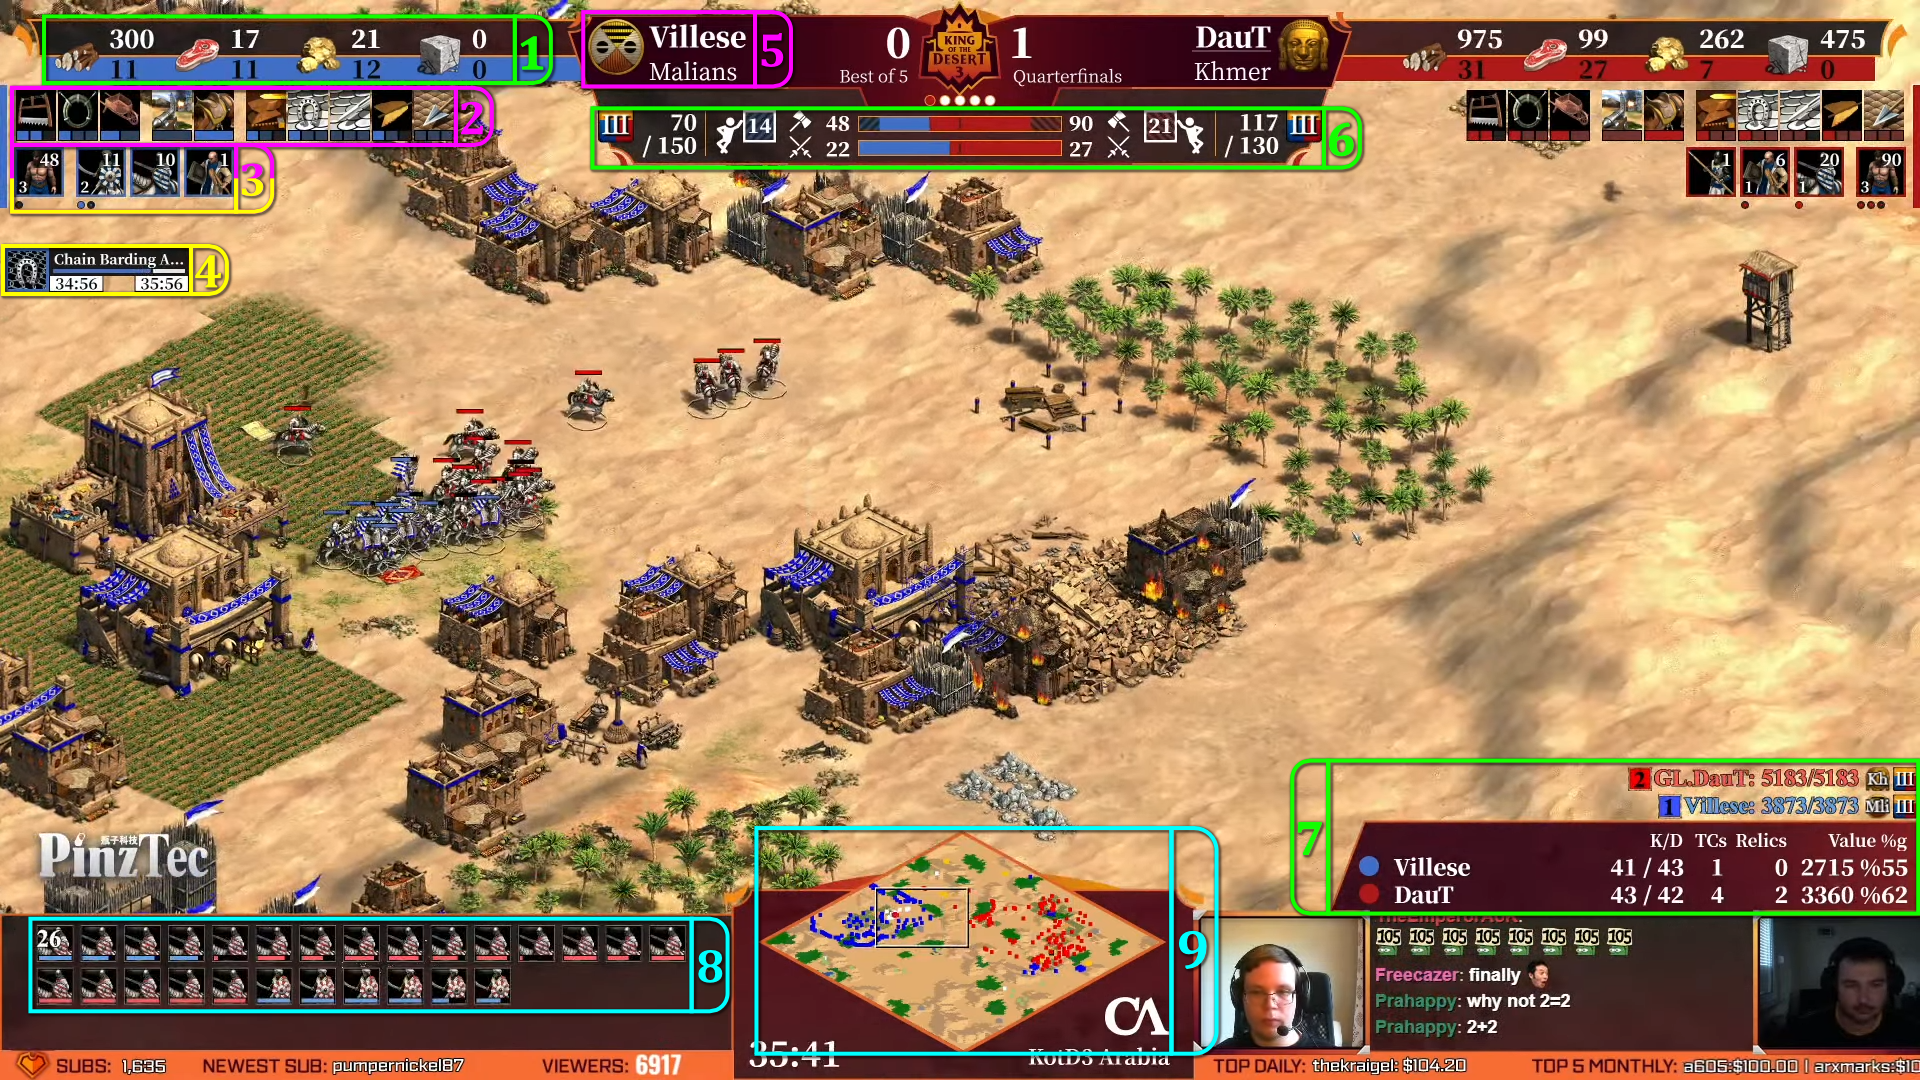
\includegraphics[width=\textwidth, height=0.9\textheight, keepaspectratio]{assets/captureage-screenshot-patches.png}
  \caption{An overview image of the CaptureAge Preview interface and its patches; see Table~\ref{tab:captureage-patches} for a description of each patch.}
  \label{img:captureage-preview}
\end{figure}
\FloatBarrier

\begin{table}[htbp]
  \centering
  \setlength{\tabcolsep}{4pt}
  \renewcommand{\arraystretch}{1.5}
  % m{} column for vertical centering, wider first col to accommodate rotated text safely
  % Use p{} instead of m{} so multirow controls the total block height cleanly
  \caption{PEAS-based patches in the CaptureAge Preview overlay. Numbers refer to Figure~\ref{img:captureage-preview}. World is intentionally added as a patch for its dual role as Environment and Actuator information, and left with no number because it is not explicitly labeled in the UI.}
  \begin{tabularx}{\textwidth}{@{}>{\centering\arraybackslash}p{0.9cm}>{\centering\arraybackslash}p{0.6cm}X X@{}}
    \toprule
    \textbf{PEAS} & \textbf{\#} & \textbf{Patch Name} \\ \midrule
    \multirow[c]{3}{0.25cm}[-1.8em]{\rotatebox[origin=c]{90}{\shortstack{Performance}}} & 1 & \textbf{Resources}: A tab showing the current amount of each resource in the player's stockpile, and the number of villagers gathering each resource. \\
    & 6 & \textbf{Key Stats Comparison}: Active age technology, total population, idle villagers, total workers, and number of military units. \\
    & 7 & \textbf{Stats Comparison}: Units killed and lost, active Town Centers, collected Relics, army value (incl. gold composition percentage). \\
    \midrule
    \multirow[c]{4}{0.25cm}[-1.5em]{\rotatebox[origin=c]{90}{\shortstack{Environment}}} & 2 & \textbf{Key Technology Status}: Status indicators for a subset of impactful technologies. \\
    & 5 & \textbf{Player Name \& Civilization}: Identifies each player and chosen civilization. \\
    & 3 & \textbf{Units (Standing)}: Number of each unit type currently deployed (top-right of each icon).\\
    & -- & \textbf{World}: All entities and terrain in the current camera view plus world overlays (entity health, building production progress). In our analysis, its main use as Environment for commentating is showing the state of the game world. \\
    \midrule
    \multirow[c]{3}{0.25cm}[-1.2em]{\rotatebox[origin=c]{90}{\shortstack{Actuators}}} & 3 & \textbf{Units (Training)}: Units currently in production (bottom-left) with progress indicators (dots). \\
    & 4 & \textbf{Technologies}: Progress toward technologies being researched. \\
    & -- & \textbf{World}: All entities and terrain in the current camera view plus world overlays (entity health, building production progress). In our analysis, its main use as Actuator for commentating is showing player actions. \\
    \midrule
    \multirow[c]{2}{0.25cm}[-1.25em]{\rotatebox[origin=c]{90}{\shortstack{Sensors}}} & 8 & \textbf{Unit Selection}: Currently selected units and their health for tactical comparison. \\
    & 9 & \textbf{Minimap}: Zoomed-out map overview for rapid spatial navigation. \\
    & -- & \textbf{Fog of War Toggle}: (Hidden control) See player's visible areas (active vision) and explored (seen, but no active vision)\\
    \bottomrule
  \end{tabularx}
  \label{tab:captureage-patches}
\end{table}

\clearpage

CaptureAge offers patches analogous to the SC2 overlay, but with persistent displays (few popups) and a more player-grouped layout. This supports both within-player interpretation (e.g., what an economy suggests about strategy) and between-player comparison (e.g., who is ahead).

Because most information is visible at all times in this CaptureAge version, we do not reconstruct explicit information-foraging paths as \citet{dodge2018} did from overlay transitions. Instead, we code utterances into Commentary Categories and Subtypes and map these to PEAS types, producing a comparable characterisation of what information supports different narrative moves.

Subtypes further specify the topic within each category. Table~\ref{tab:captureage-states} lists the Subtypes derived from the primary coding pass and their PEAS mapping.

\begin{table}[htbp]
  \begin{threeparttable}
    \caption{Subtypes derived from the T90 \& Nili coding pass, showing the AoE2-specific events and states available from CaptureAge data that casters draw on. The PEAS column indicates which information type primarily supports commentary on that event or state. A Subtype may appear in multiple Commentary Categories (e.g., a Tech State can be an Event Description when it changes, or a State Update when mentioned as context).}
    \centering
    \setlength{\tabcolsep}{4pt}
    \renewcommand{\arraystretch}{1.5}
    \begin{tabularx}{\textwidth}{@{}>{\arraybackslash}p{3.2cm}>{\arraybackslash}p{2cm}X X@{}}
      \toprule
      \textbf{Event or State}  & \textbf{PEAS-type} & \textbf{Description} \\ \midrule
      Economy Comparison   & Performance & Comparison between players on economic unit counts and allocation. \\
      Military Comparison  & Performance & Comparison between players on military unit counts and composition. \\
      Economy State        & Environment & The current state of the player's economy, including resource stockpiles and villager distribution. \\
      Military State       & Environment & The current state of the player's military, including unit and building types and numbers. \\
      Tech State           & Environment & The current state of researched technologies, including military and economic upgrades currently active. \\
      Civilization Context & Environment & The unique attributes and strategies associated with the player's chosen civilization. \tnote{1} \\
      Base Design          & Environment & The layout and design of the player's base, including defensive structures and resource placement. \\
      Age Up Progress      & Actuator  & The event of advancing to the next age, unlocking new units and technologies, marking a strategic shift. \\
      Economy              & Actuator & Other economic events, including automated events (e.g. a villager depletes resources) and moving villagers onto a resource. \\
      Movement             & Actuator & The movement of units across the map, including positioning for attacks or retreats. Either implicit (due to unit behavior) or explicit (due to player commands). \tnote{2} \\
      Tech Progress        & Actuator & The ongoing research of technologies, reflecting the player's investment in long-term strategic advantages. \\
      Unit Production      & Actuator  & The ongoing production of military units, indicating the player's strategic focus and readiness for combat. \\
      Building Production  & Actuator & The ongoing construction of buildings, reflecting the player's economic and military development. \\
      Laming               & Actuator & Stealing resources from the enemy's area, disrupting their economy. \\
      Economy Delay        & Actuator & A battle causing a delay in producing buildings or collecting resources. \\
      Eco Raid             & Actuator & Raiding the enemy's economy leading to loss of villagers. \\
      Battle               & Actuator & A battle between two armies, resulting in losses on either side. \\
      Scouting Info        & Sensors & The exploration of the map to gather information about the enemy's position and strategy. \\
      Opinion              & - & The caster's opinion on a player's strategy or decision. \\
      \bottomrule
    \end{tabularx}
    \begin{tablenotes}
    \item[1] While rooted in Environment, this draws on domain knowledge to explain significance.
    \item[2] It is not always clear if an action is implicit or explicit from watching the game, but it can be inferred from the context and the player's intentions.
    \end{tablenotes}
    \label{tab:captureage-states}
  \end{threeparttable}
\end{table}

\section{Coding}
\label{subsec:coding}
We coded three shoutcasts: one primary cast (T90 \& Nili) receiving full coding across all dimensions, and two additional casts (LidaKoR; MembTV \& Chris) coded at Category level only for validation. The primary cast provides the detailed findings; the validation casts check whether the Commentary Category distribution generalises across casters and match contexts. Full sub-type and Information Source coding is time-intensive and was not needed for validation, Category-level consistency across three independent casts is sufficient for this exploratory goal.

We selected a co-casted tournament match with two veteran casters (T90Official and NiliAoE; Table~\ref{tab:t90-nili-coding}) and, with permission, transcribed and coded all utterances. We generated an Automated Speech Recognition (ASR) draft, manually corrected it while watching the video, and manually diarized speakers. We kept utterances close to the original (removing stutters/false starts) and split long sentences into patch-aligned units (e.g., army size vs.\ technology) to capture distinct information needs. Because the CaptureAge Preview UI shows most information persistently, we cannot infer which patch a caster actually consulted; we therefore code utterances by information source (including non-patch sources such as Background Information), allowing multiple codes per utterance as in prior SC2 work \cite{dodge2018}.

Coding was performed by a single coder (the author; familiar with AoE2 and the CaptureAge overlay, and involved in its design) in multiple passes: segmentation, then Intelligibility Types (including Judgment \cite{dodge2018}), then Information Sources and Commentary Categories/Subtypes (iteratively refined with re-coding for consistency). The full final coding appears in Table~\ref{tab:t90-nili-coding}.

\section{Results}
\label{sec:prelim-analysis-results}
We report full results from the T90 \& Nili cast with light category-only validation on LidaKoR and MembTV \& Chris (Tables~\ref{tab:lidakor-coding} and~\ref{tab:memb-chris-coding}). Frequencies describe what was said, not necessarily what was most important: salient events may be rare. Because events occur in parallel \cite{lux2019} and we do not observe what casters attended to directly, we do not compute precision/recall and treat frequency as a sanity check.

\subsection{Intelligibility Types}
T90 \& Nili's cast follows the patterns reported by \citet{dodge2018}: What (52\%) is most frequent, followed by What Could Happen (17\%) and How To (9\%). Why Did (7\%) is somewhat more frequent; variation across match narratives and caster preferences in \citet{penney2021} suggests this is within an expected range. See Table~\ref{tab:lim-coding-compare}.

\subsection{Commentary Categories}
Then we looked at the different Commentary Categories used by the casters, summarized in Table~\ref{tab:communication-intents-values}. Most patch-based utterances are Event Descriptions (27\%), followed by Strategy Discussion (20\%) and Strategy Prediction (18\%). State Updates (11\%) are also frequent, while the other categories are less common. In the top three the only outlier is Strategy Discussion being the highest for Memb \& Chris, but the trend is similar across all three casts analyzed, with some variations in the less frequent categories. The full descriptions of each category can be found in Table~\ref{tab:communication-intents-descriptions}. Commentary Categories were not used by \citet{dodge2018}, so we cannot compare directly.

\begin{table}[ht!]
  \begin{threeparttable}
    \caption{Utterance type code set with AoE2 and SC2 counts\cite{dodge2018} and proportions among all tagged utterances added for comparison. }
    \begin{tabularx}{\textwidth}{@{}l|rr|rr|X@{}}
      \toprule
      \textbf{Utterance Type \tnote{a}} & \textbf{Freq SC2} & \textbf{\% of codes} & \textbf{Freq AoE2} & \textbf{\% of codes} & \textbf{Description}                                  \\ \midrule
      what                    & 595               & 44\%           & 110                & 52\%          & What the player did or anything about game state                   \\
      what could happen       & 376               & 29\%           & 37                 & 17\%          & What the player could have done or what will (not\tnote{b}) happen.\\
      how to                  & 233               & 17\%           & 20                 & 9\%          & Explaining rules, audience tips, directives, high level strategies \\
      judgment      & 112               & 8\%            & 24                 & 11\%          & Evaluation of player actions                                       \\
      why did                    & 27                & 2\%            & 14                  & 7\%           & Why the player performed an action                                 \\
      why didn't              & 6                 & 0\%            & 7                 & 3\%           & Why the player did not perform an action                           \\ \midrule
      Total\tnote{c}          & 1349              &               & 212                 &               &
    \end{tabularx}
    \label{tab:lim-coding-compare}
    \begin{tablenotes}
      \footnotesize
    \item[a] Originally slightly modified by \citet{dodge2018} from \citet{lim2009} adding the judgment category, and rephrasing others.
    \item[b] Slightly modified from \citet{dodge2018} adding a what will \textit{not} happen
    \item[c] \citet{dodge2018} reports 1024 utterances, but 1349 codes, as some utterances had multiple codes. We split up sentences (see Appendix~\ref{sec:appendix-coding} for the full utterance-level coding) based on foraging targets. \citet{dodge2018} analyzed 10 matches; we analyzed 3 matches.
    \end{tablenotes}
  \end{threeparttable}
\end{table}

\begin{table}[ht!]
  \caption{Commentary Categories counts and percentages. Percentages indicate the proportion of each strategy within each cast, and overall. Totals may not add up to 100\% due to rounding. Sorted descending by total count.}
  \centering
  \setlength{\tabcolsep}{3pt}
  \renewcommand{\arraystretch}{1.5}
  \begin{tabularx}{\textwidth}{@{}>{\raggedright\arraybackslash}p{4cm}|>{\centering\arraybackslash}p{1.2cm}>{\raggedleft\arraybackslash}p{1.2cm}|>{\centering\arraybackslash}p{1.2cm}>{\raggedleft\arraybackslash}p{1.2cm}|>{\centering\arraybackslash}p{1.2cm}>{\raggedleft\arraybackslash}p{1.2cm}|>{\centering\arraybackslash}p{1.2cm}>{\raggedleft\arraybackslash}p{1.2cm}@{}}
    \toprule
    \textbf{Category}  & \multicolumn{2}{c|}{\centering\textbf{T90 \& Nili}} & \multicolumn{2}{c|}{\centering\textbf{LidaKoR}} & \multicolumn{2}{c|}{\centering\textbf{Memb \& Chris}} & \multicolumn{2}{c}{\centering\textbf{Total}} \\
    & \textbf{N} & \textbf{\%} & \textbf{N} & \textbf{\%} & \textbf{N} & \textbf{\%} & \textbf{N} & \textbf{\%} \\ \midrule
    Event Description      & 85 & 31\% & 69 & 26\% & 66 & 21\% & 220 & 26\% \\
    Strategy Discussion    & 37 & 14\% & 42 & 16\% & 90 & 29\% & 169 & 20\% \\
    Strategy Prediction    & 34 & 13\% & 74 & 28\% & 40 & 13\% & 148 & 18\% \\
    State Update           & 12 & 4\% & 34 & 13\% & 44 & 14\% & 90 &  11\% \\
    Civilization Analysis  & 14 & 5\% & 12 & 5\% & 22 & 7\% & 48 &  6\% \\
    Historical Account     & 16 & 6\% & 4 &  2\%  & 16 & 5\% & 36 &  4\% \\
    Game Discussion       & 24 & 9\% & 0 &  0\%  & 7 &  2\% & 31 &  4\% \\
    Off-Topic  & 16 & 6\% & 0 &  0\%  & 6 &  2\% & 22 &  3\% \\
    Player Analysis     & 10 & 4\% & 11 &  4\% & 0 &  0\% & 21 &  2\% \\
    Map Analysis              & 1 &  0\%  & 9 &  3\%  & 6 &  2\% & 16 &  2\% \\
    Technical Issues        & 6 &  2\%  & 3 &  1\%  & 2 &  1\% & 11 &  1\% \\
    Recap        & 5 &  2\%  & 2 &  1\%  & 3 &  1\% & 10 &  1\% \\
    Skill Discussion           & 3 &  1\%  & 1 &  0\%  & 5 &  2\% & 9 &   1\% \\
    Joke        & 6 &  2\%  & 1 &  0\%  & 1 &  0\% & 8 &   1\% \\
    Match Introduction       & 1 &  0\%  & 3 &  1\%  & 2 &  1\% & 6 &   1\% \\
    \bottomrule
  \end{tabularx}
  \label{tab:communication-intents-values}
\end{table}

Looking at the Subtypes for Event Descriptions (Table~\ref{tab:event-frequencies}), which most closely describe the foraging Cues, we find that most events described are Battles (16), followed by Economic Building (9), Scouting (4), and Movement (3). This order is mostly in line with the findings of the occurrence matrix of Actions for the SC2 analysis, although unit production specifically was only mentioned once in the AoE2 match we analyzed (but the original methodology used by \citet{dodge2018} does not distinguish between building and unit production).

\subsection{Information Sources}
To clarify which information sources the prototype needs, we examine the sources used in the coded utterances. We find that most utterances rely on Descriptive Information (92), followed by Domain Knowledge (55) and Analytical Knowledge (46) (See Table~\ref{tab:info-sources-frequencies}). In the co-occurrence matrix (Table~\ref{tab:co-occurrence-type-source}), Event Descriptions and State Updates mostly rely on Descriptive Information, while Strategy Discussion and Prediction rely more on Domain and Analytical Knowledge. We also checked the co-occurrence of intelligibility types with Information Sources, but the only clear pattern is that What questions mostly rely on Descriptive Information (83/101), while the rest rely on a mix of the other Information Sources.

\subsection{Narrative Overview}

Below we describe short passages to illustrate how the casters explain events and draw on different information sources to support the narrative. Table~\ref{tab:t90-nili-example-forward-tower} illustrates how T90 \& Nili detect a Tower Rush strategy and mix prediction and context with event description.

\begin{table}[!htbp]
  \caption{T90 \& Nili describing the moment they detect the tower rush strategy by Villese, and its implications.}
  \label{tab:t90-nili-example-forward-tower}
  \centering
  \setlength{\tabcolsep}{4pt}
  \renewcommand{\arraystretch}{1.3}
  \begin{tabularx}{\textwidth}{@{}l>{\raggedright\arraybackslash}p{7cm}>{\raggedright\arraybackslash}p{4cm}>{\centering\arraybackslash}p{2cm}@{}}
    \toprule
    \textbf{Speaker} & \textbf{Utterance} & \textbf{Explanation} & \textbf{PEAS/Info Type} \\
    \midrule
    T90 & I know it's not common, but if this was a player like Vivi and Vivi scouted that, uh, villagers were on gold, I think Vivi would come forward and tower there. I think he would tower right outside the gold because it's going to take forever for DauT to make the archers, and DauT would have no real defense to a forward. & Analysis and background information, filling in lull for entertainment, based on game state. & Background Information \\
    T90 & And here comes Villese. Villagers forward from Villese. & A Cue, then describing what actually happens in the game, indicator of predicted action. & Actuator \\
    T90 & He's going to tower right outside the gold. & Predicting what will happen, explaining significance for less experienced viewers. & Environment \\
    Nili & Oh, what's this? Pressure on the gold there. That is indeed maybe taking him by surprise. & Emphasizing the surprise element, building excitement. & Environment \\
    Nili & The scout is there. Does he see it? & Discussing the next event, related to previous. & Sensors \\
    \bottomrule
  \end{tabularx}
\end{table}

In Table~\ref{tab:t90-nili-example-forward-tower} they first fill a lull in the action with some speculation (more common at the start of a match). Then an event happens; they predict how it will play out, describe that event, and add context either by foraging or by predictions (predictions were not noted explicitly in SC2 \cite{dodge2018}). Notably, Event Descriptions often follow a cue/event \(\rightarrow\) context \(\rightarrow\) continued description pattern, aligning with the A--E--P+S structure: Actuator to describe what is happening, Environment to provide context to what might happen next, then continue with Performance or Sensors information.

\begin{table}[!htbp]
  \caption{LidaKoR describing the moment they detect the tower rush strategy by Villese, and its implications.}
  \label{tab:lidakor-example-forward-tower}
  \centering
  \setlength{\tabcolsep}{4pt}
  \renewcommand{\arraystretch}{1.3}
  \begin{tabularx}{\textwidth}{@{}l>{\raggedright\arraybackslash}p{7cm}>{\raggedright\arraybackslash}p{4cm}>{\centering\arraybackslash}p{2cm}@{}}
    \toprule
    \textbf{Speaker} & \textbf{Utterance} & \textbf{Explanation} & \textbf{PEAS/Info Type} \\
    \midrule
    LidaKoR & DauT is adding, uh, just one range right now, whereas... <cut-off> & Describing the state of the game & Environment \\
    LidaKoR & So that is a men-at-arms towers play from Villese, in fact, a forward archery range. & Cutting to a detected event & Actuator \\
    LidaKoR & So probably a few skirmishers will be out right now. & Predicting what will happen, based on the pre cut-off event & Environment \\
    LidaKoR & Malian men-at-arms will have, uh, extra pierce armor, & Providing context about a civilization advantage & Environment \\
    LidaKoR & And it appears that Villese is going to be able to force DauT off from gold & Describing the next event & Actuator \\
    \bottomrule
  \end{tabularx}
\end{table}

The same event is described by LidaKoR in Table~\ref{tab:lidakor-example-forward-tower}. While he notices slightly later, he follows a similar pattern: he describes state, pivots to the detected event (Actuator), infers implications (Environment), adds Domain Knowledge about civilization mechanics, then continues with the unfolding event. While civilization is part of the Environment, its role as knowledge/context is distinct from direct state.

Most Event Descriptions concern battles and building production (Table~\ref{tab:event-frequencies}), with other events being less common.

Historical and background information is added during lulls, particularly at the start. This also happens in StarCraft II. In the first match\footnote{\url{https://www.youtube.com/watch?v=ArFjdP7nkTU}} listed in \citet{dodge2018}'s research, we found that casters add information from other matches and from meta progression (how the game's gameplay evolves) to contextualize players’ habits and match trajectory; references to plays from other matches are also common.

In AoE2, T90 \& Nili open with player/location context and background information, then move through a cue-driven event loop that follows the A–E–P+S structure. Lulls are filled with state updates or other contextual information; new cues often interrupt context, with casters returning to finish the thought.

Unlike T90 \& Nili, LidaKoR and MembTV \& Chris discuss map layout as part of the introduction (key resource locations and terrain features and their strategic implications). In the corresponding segment, T90 \& Nili instead thank sponsors, which is obligatory and took precedence.

These observations suggest the top-level narrative structure in Figure~\ref{fig:shoutcasting-structure}: introductions, then an event-driven loop interspersed with state updates and knowledge sharing during lulls.

\begin{figure}[htbp]
  \centering
  % Avoid build errors if file is missing
  \IfFileExists{assets/shoutcasting-structure.pdf}{%
    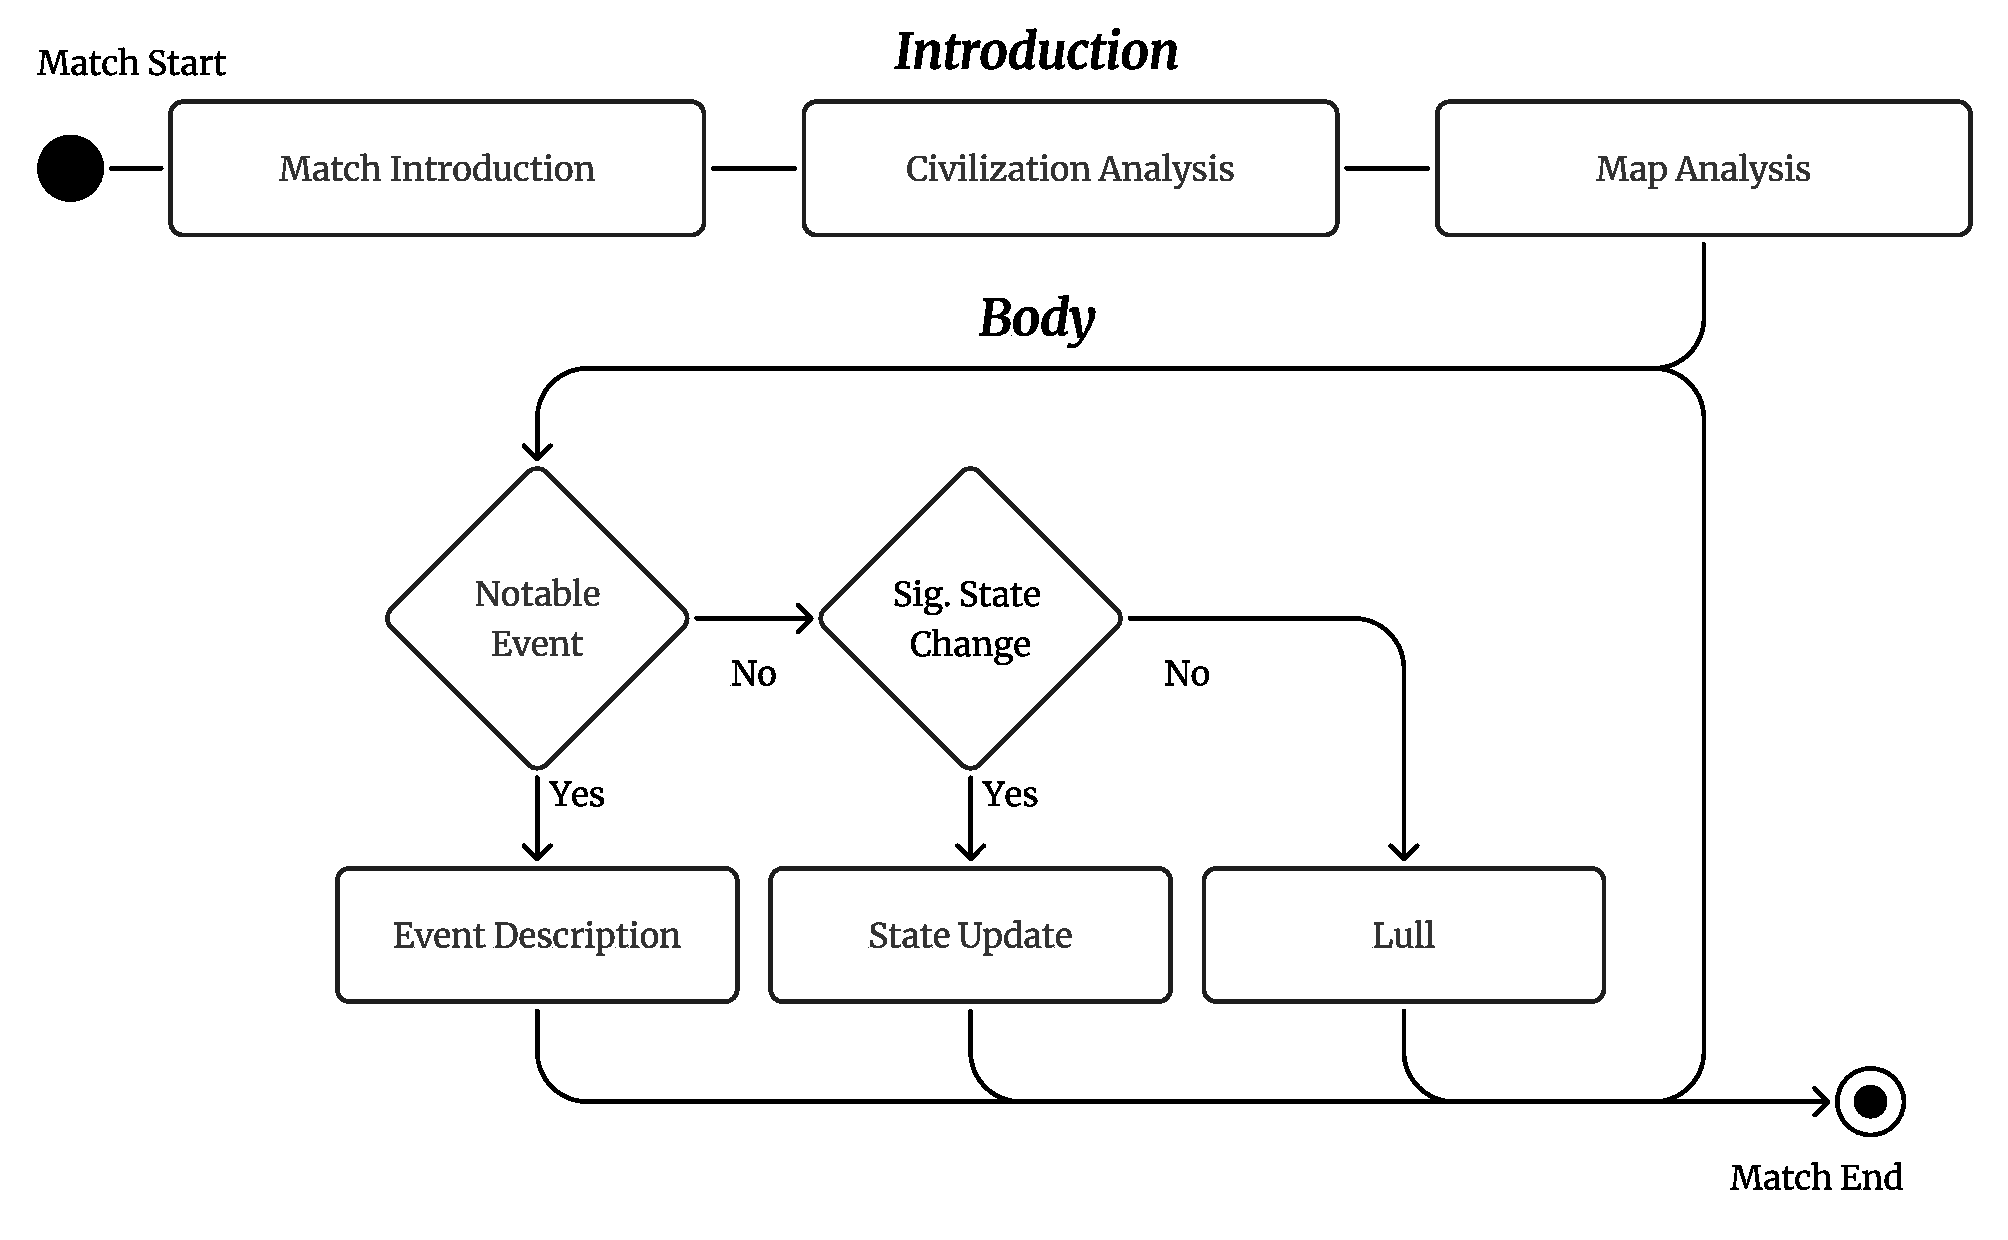
\includegraphics[width=\textwidth]{assets/shoutcasting-structure.pdf}%
  }{%
    \fbox{\parbox{0.95\textwidth}{\centering Placeholder: missing file\\`assets/shoutcasting-structure.pdf`}}%
  }
  \caption{Top-level narrative overview of shoutcasting structure observed across the analyzed casts. It starts with introductions, followed by a loop driven by events, interspersed with state updates and knowledge sharing during lulls.}
  \label{fig:shoutcasting-structure}
\end{figure}

\subsection{Other Observations}
Two recurring themes in the T90 \& Nili cast are consistent with prior findings on esports commentary \cite{lux2019, cheung2011starcraft}. First, T90 \& Nili frequently note the amount of attention points that players need to keep track of and how much is going on, which is in line with \citet{lux2019}'s views on attention points:
\begin{quote}
  \textbf{T90:} \textit{So he’s trying to do a lot right now, and even if he doesn’t want the full wall at this time, he has two idles simply due to how much he’s trying to juggle at the moment.}
\end{quote}
Here Villese is so busy he cannot fully focus on building his wall, leading to idle villagers. This highlights the high cognitive load players are under due to the many attention points they need to keep track of.

Casters also discuss information asymmetry, a key finding of \citet{cheung2011starcraft}. Scouting remarks such as "Does he see it?" highlight cases where casters know more than the player (\textit{Unknown to player, known to caster}):
\begin{quote}
  \textbf{Nili:} \textit{Yeah, that is sometimes the funny situation as a caster, right? We kind of don’t want to lie to our viewers and we kind of want to say, "Okay, what are the next steps to come back?"}\\
  \textbf{Nili:} \textit{Obviously for us, we get the intel, we see everything, we know how bad it looks.}
\end{quote}

This illustrates a common situation: casters see the likely outcome while players lack information. While anecdotal, it suggests these dynamics also hold in AoE2 and are salient to casters.

The other asymmetry types in \citet{cheung2011starcraft} also appear. Players and casters may be uncertain about battle outcomes (\textit{Unknown to player, unknown to caster}):

\begin{quote}
  \textbf{T90:} \textit{Yeah, he should easily clear that, but I think DauT will be happy with how long it took Villese to decide to take that fight, and it wasn’t quite as convincing as I thought it would be either.}
\end{quote}
Here the casters expected a clearer outcome, highlighting uncertainty even for experienced commentators.

Predictions reflect the final asymmetry (\textit{Known to player, unknown to caster}), e.g., forecasting where Villese will place a forward tower.

Because shoutcasts are audiovisual, casters often rely on what viewers see and focus their speech on salient details and transitions, sometimes reflecting only on the beginning and end states of an event.

\section{Discussion}

\subsection{\textbf{RQA1:} How similar is AoE2 to StarCraft II in terms of information and commentary strategies?}
Intelligibility Types (Table~\ref{tab:lim-coding-compare}) and information-foraging patterns (A--E--P+S) closely match SC2 shoutcasting \cite{dodge2018}, confirming that core commentary patterns transfer across RTS titles as an exploratory finding. Because these patterns differ from non-game systems \cite{lim2009}, the similarity appears to reflect RTS/shoutcasting characteristics rather than coincidence, and supports an event-driven prototype grounded in the same frameworks.

\subsection{\textbf{RQA2:} What information and knowledge are used to commentate on these match events?}
Commentary is grounded in \textit{Descriptive} information and enriched with \textit{Domain} and \textit{Analytical} knowledge (Table~\ref{tab:co-occurrence-type-source}). Event Descriptions and State Updates mostly rely on Descriptive information, while Strategy Discussion and Prediction draw more on Domain and Analytical knowledge. For a prototype, this implies detecting actuator-level events (especially battles and key production) and interleaving concise state updates, integrating these layers.

\subsection{\textbf{RQA3:} What narrative structure is used to report on a competitive AoE2 match?}
Figure~\ref{fig:shoutcasting-structure} suggests a recurring event-driven cycle: introductions (match, players, civilizations, map), then cue-driven event reporting enriched with context; lulls are filled with state updates or background knowledge. Two key challenges for an automated system follow:
\begin{enumerate}[noitemsep, topsep=0pt]
  \item Prioritize narratively critical events; frequency is not importance (e.g., a single ``castle drop''---an aggressive forward castle---can outweigh many minor skirmishes).
  \item Handle simultaneous events via summarization or salience selection rather than detailing everything.
\end{enumerate}
These constraints motivate prioritization and concurrency handling (e.g., via summarization or salience selection) in the prototype.

\subsection{Synthesis}
Our AoE2 shoutcasting analysis suggests a cyclical, event-driven pattern: descriptive cues enriched with domain/analytical context. To design a useful system, we must identify which event types and knowledge updates AoE2 viewers value, how to balance action reporting with strategic contextualization, and whether summarization approaches yield coherent narratives. These questions are addressed in the preliminary viewer study (Chapter~\ref{chap:viewer-study}).

\subsection{Limitations}
We did not assess inter-rater reliability as in \citet{dodge2018}: coding was performed by a single coder, and segmentation choices may bias frequencies. We also analyzed only three shoutcasts, limiting generalizability, though the similarity to SC2 suggests the core patterns may transfer within RTS shoutcasting.

Our prototype is text-based, but the analyzed domain is audiovisual: casters rely on what viewers see and may omit details that are visually available. If anything, this may understate Actuator/What content, strengthening the rationale for event-driven summaries.

Finally, we still lack a principled answer to summarization itself: which events matter, and what supporting information is required for a coherent narrative. Event cues interrupt context, but that does not imply contextual information is unimportant. This is best explored through an additional exploratory viewer study, which we conduct in Chapter~\ref{chap:viewer-study}.

\chapter{Preliminary Viewer Study}\label{chap:viewer-study}
The domain comparison in Chapter~\ref{chap:prelim} leaves AoE2-specific questions about which event types matter, how to balance action-focused and contextual content, and whether event-driven summaries remain coherent. To align the prototype with viewer needs (beyond caster practice) \cite{penney2021}, we conducted a user study.

\section{Goals}

We aim to (a) identify which event types and knowledge updates viewers consider essential, (b) understand preferences for action-focused vs.\ contextual content, and (c) assess whether an event-driven summary can still produce a coherent narrative. We deliberately omit linguistic quality and engagement here because the summaries are assembled from existing shoutcasts and would confound content with stylistic variability; these aspects are better assessed later in a controlled prototype evaluation. Instead, we focus on perceived content relevance and narrative coherence.

To guide the study, we focus on three research questions derived from the domain analysis, addressing the second part of RQ4 from Chapter~\ref{chap:introduction}, which content types viewers find most relevant:
\begin{enumerate}[noitemsep, topsep=0pt]
  \item \textbf{RQB1: Which events and knowledge updates are most important to include in a summary?} Which event sub-types and supporting state updates are valued by viewers, and does contextual information such as predictions improve understanding?
  \item \textbf{RQB2: How should different types of content be balanced to maintain viewer interest?} Commentary spans action-focused events and contextual strategic or skill-based content; we aim to understand the preferred balance.
  \item \textbf{RQB3: To what extent can an event-driven summary produce a coherent and understandable narrative?} We evaluate whether a summary constructed from key events enables viewers to follow the match narrative.
\end{enumerate}

\section{Experimental Design}
To answer these questions we conduct a user study, showing viewers a short summary video. This section describes the experimental design of this exploratory study.

\subsection{Design Overview}
We presented participants with a short hand-made summary video\footnote{\url{https://youtu.be/x-otkWbBBdc}}. Video is familiar to viewers and lets us focus on content and narrative structure without introducing the additional factor of a new medium (text).

The summary was assembled from a real match shoutcast by MembTV (Villese vs DauT), chosen for its shorter length, single-caster format, and clear production cues (a DauT Castle \footnote{A partially built defensive structure, investing significant resources, but never making it to completion, leaving it essentially useless. Named after the player known for this risky play}). We included subtitles for accessibility and to mitigate variability in audio quality, video-editing/cutting artifacts, and accents. Although we do not focus on linguistic aspects, we chose MembTV because his casting style is broadly compatible with the kinds of play-by-play and incremental reporting patterns described in live text commentary \cite{lewandowski2012, pavzanin2022}.

Then players were asked to answer several questions in a questionnaire (operationalization notes in Appendix \ref{appendix:prelim-operationalization}; full item wordings in Appendix \ref{appendix:prelim-questionnaire}), based on the Commentary Categories and sub-types we found in the shoutcaster analysis. The Commentary items (C-set) cover intro context, battle variants (delay, military losses, villager kills, break-ins, overwhelming), scouting and uncommon events, key state updates (age-ups, military tech), and limited contextual content (situation-specific information, predictions). Technologies are treated as state updates rather than standalone events. The General items (G-set) capture broader preferences for action, strategy, and skill content and attitudes toward summaries vs. full matches. Because our coding was coarse and based on a small set of matches, C-set selections were refined using the author’s domain experience while remaining grounded in the A–E–P+S loop and adapted to the chosen video.

The specific procedure was as follows: First participants consented, followed by; viewing habits and skill level (O-items 1--3); watch the summary; report whether they had watched the match before; rate C-items, then G-items; provide optional open feedback and prior-exposure items (O-items 4--5). The questionnaire was posted on \texttt{r/aoe2}, chosen as the recruitment channel because esports subreddits have been shown to yield substantial respondent pools for studies targeting this audience \cite{hamari2017, bidermayer2020}. The survey ran from March 5th to March 8th, 2021.

\subsection{Survey Design}
The question set was not fully comprehensive with the findings from the Commentary Categories and sub-types we found in the shoutcaster analysis to balance coverage with respondent fatigue. Some values prominent in CaptureAge were omitted (e.g., economy state updates and army balance), with the assumption that these would be relevant regardless. In our sample, most production-related reporting concerned uncommon building constructions (e.g., forward placement), so we grouped this with other uncommon events (e.g., Siege Tower hops). We also asked about summary quality, adapting phrasing to the video format.

Full item wordings for the questionnaire are provided in Appendix~\ref{appendix:prelim-questionnaire}. The Commentary questions (C-set) asked participants to rate the relevance of specific commentary content types on a 5-point Likert scale (Not Relevant, Slightly Relevant, Relevant, Very Relevant, Required), covering intro context, multiple battle types, scouting and uncommon events, key state updates (age-up timings, military tech), plus predictions and situation-specific knowledge. The General questions (G-set) used a 5-point agreement scale (plus a Does-not-apply option) to capture perceived understanding of the summary, attitudes toward summaries vs.\ full matches and time constraints, content preferences (battles/strategy/skill), and perceived impact of video-cutting artifacts. The other questions (O-set) captured self-reported competence, Elo bracket \footnote{Elo is a rating system used in the game to calculate the relative skill levels of players in matches to match opponents of similar strength -- used as a mathematical proxy for skill level.}, viewing frequency, prior exposure, and an open-ended feedback prompt.
Ethical clearance was obtained from the university ethics board (reference RP~2021-36).

\section{Results}
We report participants, analysis approach, and results for the C-set and G-set items.

\subsection{Participants}
57 respondents participated. Five reported no 1v1 AoE2:DE ranked rating (indicating they do not play competitively); for the remaining 52 we used the midpoint of their reported Elo range, yielding a sample with slightly elevated skill ($M = 1282$, $SD = 210$), above the average player base. All respondents watched competitive AoE2 at least monthly; most watched daily ($n=30$, 53\%). The majority had not watched the specific stimulus match before (No: 63\%, Yes: 23\%, Unsure: 14\%). This represents a sample of frequent-viewing, skill-elevated participants appropriate for informing design aimed at the core viewer audience, though less representative of casual viewers.
For Other (O) responses "Does not apply" were omitted from analysis (as indicated by $N$). We did not ask for demographic information to maximize privacy and encourage participation, so we cannot report on age, gender, geographical distribution, or other demographic factors.

\subsection{Statistical Analysis}
Ratings were collected on a 5-point Likert scale and treated as approximately continuous. Using R\footnote{R Version 4.5.1 (2025-06-13), lme4 v1.1.37, emmeans v1.11.2.8}, we fit separate linear mixed-effects models ($lme4$; REML) for each dataset with fixed item cell-means  (testing within each item) and a random intercept for participants (normalizing participant bias) ($itemScore \sim 0 + item + (1|Participant)$). Estimated marginal means (EMMs; $emmeans$) were tested against prespecified anchors (3, 3.5, 4, to test if means significantly differed from these values on a 5-point scale) to understand if the values differed significantly from of these values. Inference used Satterthwaite degrees of freedom ($lmerTest$). Because the analysis was exploratory by testing against three different anchors, we controlled the false discovery rate using Benjamini--Hochberg (BH) separately within each data set (C \& G). BH adjustment did not change any statistical decisions relative to raw p-values at $\alpha = .05$; we therefore report BH-adjusted p-values. Analysis scripts and an anonymized dataset are available online\footnote{See Appendix~\ref{app:preliminary-analysis} for public links to analysis scripts and dataset}.

\subsection{Additional Checks}
\label{subsec:additional-checks}
The G-set model produced a boundary singular fit: the participant random-intercept variance converged to zero, indicating no detectable between-participant differences after accounting for item means. This is equivalent to a plain linear model for that dataset; fixed-effect estimates and standard errors are unaffected. Indicating participants did not differ systematically in how they rated the general preference items; any variation was item-specific rather than a stable individual tendency.

Residual diagnostics (Q--Q plots, histogram) indicated mild tails/outliers and a slight left skew; given the robustness of Gaussian LMMs to moderate non-normality, we proceeded.
We also tested whether perceived technical issues with the video (e.g., caused by video cutting a pre-existing shoutcast), \textit{TechnicalIssues}, self-reported skill (\textit{CompetenceSelf}, \textit{CompetenceELO}), viewing frequency (\textit{WatchFrequency}), or prior exposure (\textit{WatchedBefore}) influenced C-set or G-set ratings. No covariates were significant (none of the aforementioned items affect the items of the C-set or G-set) after Benjamini--Hochberg adjustment within dataset (all $p_{BH} \ge .094$). Raw p-values suggested potential interactions for \textit{TechnicalIssues} and \textit{WatchedBefore} in the G-set ($p = .019$ and $p = .038 < \alpha$), but these did not survive BH adjustment ($p_{BH} = .094 > \alpha$). So video quality issues, prior exposure to the specific match, and skill level did not reliably shift what content participants rated as relevant, the ratings reflect content preferences rather than study artifacts.

\begin{table}[h!]
  \centering
  \caption{Commentary content items (C-set): Estimated marginal means (EMMs), Satterthwaite degrees of freedom (df), 95\% confidence intervals, and BH-adjusted tests against nulls 3, 3.5, and 4. Each cell shows estimate/statistic (top) and adjusted p-value (bottom). p-values are Benjamini--Hochberg adjusted within the C-set. Values in bold indicate significant differences from the null at $\alpha = .05$.}
  \label{tab:results-events}
  \setlength{\tabcolsep}{4pt}
  \renewcommand{\arraystretch}{1.8}
  \begin{tabular}{lccccccc}
    \toprule
    Item & \makecell{EMM \\ (SE)} & df & \makecell{95\% CI \\ (Lower -- Upper)} & \makecell{t vs 3 \\ (p)} & \makecell{t vs 3.5 \\ (p)} & \makecell{t vs 4 \\ (p)} \\
    \midrule
    BattleEcoKills & \makecell{4.35 \\ (0.13)} & 456 & \makecell{4.09 -- 4.61} & \makecell{\textbf{10.28} \\ < .001} & \makecell{\textbf{6.48} \\ < .001} & \makecell{\textbf{2.67} \\ 0.012} \\
    IntroLayout\footnote{IntroLayout scores slightly higher than StateAgeUp, but after rounding they report the same values.} & \makecell{4.11 \\ (0.13)} & 456 & \makecell{3.85 -- 4.36} & \makecell{\textbf{8.41} \\ < .001} & \makecell{\textbf{4.61} \\ < .001} & \makecell{0.80 \\ 0.489} \\
    StateAgeUp & \makecell{4.11 \\ (0.13)} & 456 & \makecell{3.85 -- 4.36} & \makecell{\textbf{8.41} \\ < .001} & \makecell{\textbf{4.61} \\ < .001} & \makecell{0.80 \\ 0.489} \\
    StateMilTech & \makecell{4.07 \\ (0.13)} & 456 & \makecell{3.81 -- 4.33} & \makecell{\textbf{8.15} \\ < .001} & \makecell{\textbf{4.34} \\ < .001} & \makecell{0.53 \\ 0.651} \\
    BattleMilitary & \makecell{4.04 \\ (0.13)} & 456 & \makecell{3.78 -- 4.29} & \makecell{\textbf{7.88} \\ < .001} & \makecell{\textbf{4.07} \\ < .001} & \makecell{0.27 \\ 0.826} \\
    BattleOverwhelm & \makecell{3.98 \\ (0.13)} & 456 & \makecell{3.72 -- 4.24} & \makecell{\textbf{7.48} \\ < .001} & \makecell{\textbf{3.67} \\ < .001} & \makecell{-0.13 \\ 0.914} \\
    EventScouting & \makecell{3.95 \\ (0.13)} & 456 & \makecell{3.69 -- 4.21} & \makecell{\textbf{7.21} \\ < .001} & \makecell{\textbf{3.41} \\ 0.001} & \makecell{-0.40 \\ 0.738} \\
    BattleBreakIn & \makecell{3.84 \\ (0.13)} & 456 & \makecell{3.58 -- 4.10} & \makecell{\textbf{6.41} \\ < .001} & \makecell{\textbf{2.60} \\ 0.014} & \makecell{-1.20 \\ 0.304} \\
    IntroCivs & \makecell{3.81 \\ (0.13)} & 456 & \makecell{3.55 -- 4.07} & \makecell{\textbf{6.14} \\ < .001} & \makecell{\textbf{2.34} \\ 0.028} & \makecell{-1.47 \\ 0.194} \\
    Knowledge & \makecell{3.61 \\ (0.13)} & 456 & \makecell{3.36 -- 3.87} & \makecell{\textbf{4.67} \\ < .001} & \makecell{0.87 \\ 0.469} & \makecell{\textbf{-2.94} \\ 0.006} \\
    BattleDelay & \makecell{3.60 \\ (0.13)} & 456 & \makecell{3.34 -- 3.85} & \makecell{\textbf{4.54} \\ < .001} & \makecell{0.73 \\ 0.521} & \makecell{\textbf{-3.07} \\ 0.004} \\
    EventUncommon & \makecell{3.51 \\ (0.13)} & 456 & \makecell{3.25 -- 3.77} & \makecell{\textbf{3.87} \\ < .001} & \makecell{0.07 \\ 0.947} & \makecell{\textbf{-3.74} \\ < .001} \\
    IntroEconomy & \makecell{3.37 \\ (0.13)} & 456 & \makecell{3.11 -- 3.63} & \makecell{\textbf{2.80} \\ 0.008} & \makecell{-1.00 \\ 0.396} & \makecell{\textbf{-4.81} \\ < .001} \\
    IntroPlayers & \makecell{2.86 \\ (0.13)} & 456 & \makecell{2.60 -- 3.12} & \makecell{-1.07 \\ 0.368} & \makecell{\textbf{-4.87} \\ < .001} & \makecell{\textbf{-8.68} \\ < .001} \\
    Predictions & \makecell{2.51 \\ (0.13)} & 463 & \makecell{2.25 -- 2.77} & \makecell{\textbf{-3.70} \\ < .001} & \makecell{\textbf{-7.48} \\ < .001} & \makecell{\textbf{-11.26} \\ < .001} \\
    \bottomrule
  \end{tabular}
  \renewcommand{\arraystretch}{1}
  \setlength{\tabcolsep}{6pt}
\end{table}

\subsection{General Preferences}
Several G-items are significantly above 3 ("Neutral"), including \textit{PreferFullGames} ($EMM = 4.34$, $p < 0.0001 < \alpha$), \textit{LimitedTime} ($EMM = 3.58$, $p < 0.0001$), \textit{Understanding} ($EMM = 4.18$, $p < 0.0001$), \textit{TechnicalIssues} ($EMM = 3.39$, $p = 0.0069$), \textit{InterestStrategy} ($EMM = 4.64$, $p < 0.0001$), and \textit{InterestSkill} ($EMM = 4.02$, $p < 0.0001$). \textit{SummaryOpinion} is not significantly above neutral ($EMM = 3.18$, $p = 0.2358$), and large battles are not either (\textit{InterestBattles}, $EMM = 2.91$, $p = 0.5652$). Participants strongly prefer full matches but acknowledge time constraints, which opens a use case for summaries, yet they are not inherently enthusiastic about summaries as a format. Content-wise, strategy and skill dominate interest; raw battle action on its own does not stand out. Participants reported good comprehension of the event-driven summary (Understanding well above neutral), suggesting the format was sufficiently coherent even in prototype form. See Table~\ref{tab:results-general}.

\begin{table}[h!]
  \centering
  \caption{General questions (G-set): Estimated marginal means (EMMs), Satterthwaite degrees of freedom (df), 95\% confidence intervals, and BH-adjusted tests against nulls 3, 3.5, and 4. p-values are Benjamini--Hochberg adjusted within the G-set.}
  \label{tab:results-general}
  \setlength{\tabcolsep}{4pt}
  \renewcommand{\arraystretch}{1.8}
  \begin{tabular}{lccccccc}
    \toprule
    Item & \makecell{EMM \\ (SE)} & df & \makecell{95\% CI \\ (Lower -- Upper)} & \makecell{t vs 3 \\ (p)} & \makecell{t vs 3.5 \\ (p)} & \makecell{t vs 4 \\ (p)} \\
    \midrule
    PreferFullGames & \makecell{4.34 \\ (0.14)} & 441 & \makecell{4.07 -- 4.61} & \makecell{\textbf{9.79} \\ < .001} & \makecell{\textbf{6.13} \\ < .001} & \makecell{\textbf{2.48} \\ 0.019} \\
    Understanding & \makecell{4.18 \\ (0.14)} & 441 & \makecell{3.91 -- 4.45} & \makecell{\textbf{8.61} \\ < .001} & \makecell{\textbf{4.96} \\ < .001} & \makecell{1.31 \\ 0.236} \\
    LimitedTime & \makecell{3.58 \\ (0.14)} & 441 & \makecell{3.31 -- 3.85} & \makecell{\textbf{4.21} \\ < .001} & \makecell{0.59 \\ 0.578} & \makecell{\textbf{-3.03} \\ 0.004} \\
    TechnicalIssues & \makecell{3.39 \\ (0.14)} & 441 & \makecell{3.12 -- 3.65} & \makecell{\textbf{2.85} \\ 0.007} & \makecell{-0.84 \\ 0.458} & \makecell{\textbf{-4.53} \\ < .001} \\
    SummaryOpinion & \makecell{3.18 \\ (0.14)} & 441 & \makecell{2.91 -- 3.44} & \makecell{1.29 \\ 0.236} & \makecell{\textbf{-2.39} \\ 0.023} & \makecell{\textbf{-6.08} \\ < .001} \\
    \hline
    InterestStrategy & \makecell{4.64 \\ (0.14)} & 441 & \makecell{4.37 -- 4.91} & \makecell{\textbf{12.01} \\ < .001} & \makecell{\textbf{8.35} \\ < .001} & \makecell{\textbf{4.70} \\ < .001} \\
    InterestSkill & \makecell{4.02 \\ (0.14)} & 441 & \makecell{3.75 -- 4.29} & \makecell{\textbf{7.37} \\ < .001} & \makecell{\textbf{3.75} \\ < .001} & \makecell{0.13 \\ 0.895} \\
    InterestBattles & \makecell{2.91 \\ (0.14)} & 441 & \makecell{2.65 -- 3.18} & \makecell{-0.65 \\ 0.565} & \makecell{\textbf{-4.33} \\ < .001} & \makecell{\textbf{-8.02} \\ < .001} \\
    \bottomrule
  \end{tabular}
  \renewcommand{\arraystretch}{1}
  \setlength{\tabcolsep}{6pt}
\end{table}

\subsection{Events}
Nearly all C-items are significantly above 3 ("Relevant"), except \textit{IntroPlayers} ($EMM = 2.86$, $p = 0.368$) and \textit{Predictions} ($EMM = 2.51$, $p < 0.001$), where \textit{Predictions} was also significantly below the middle point. Only \textit{BattleEcoKills} exceeds 4 ("Very Relevant"; EMM = 4.35, $p = 0.012$). This indicates that viewers want to hear about almost every event type we tested except for player intros and predictions are unwanted. Among everything we asked about, battles that result in economic unit kills are the single most valued content type. See Table~\ref{tab:results-events}.

24 participants answered the optional open question about missing information. Repeated themes were missing economy/technology information (13), technical limitations (overlay density, disruptive cuts, casting style; 6), and missing win-condition/progress explanations (5). The dominant request for economic and win-condition context directly reinforces the quantitative finding that battle events are most valued when framed by their consequences; viewers want events framed by their consequences: what happened, and why it matters for the match.

\section{Discussion}

Participants preferred full matches but reported limited time, suggesting summaries could be useful if they prioritize what viewers care about most; overall attitudes toward summaries were neutral to slightly positive despite prototype limitations.

\subsection{RQB1: Which events and knowledge updates are most important to include in a summary?}

Ratings suggest a hierarchy: battles that lead to economic unit kills were most important, followed by map layout, state updates, larger battle events, and scouting. This emphasizes the consequences of battles, supported by scouting and state updates, and aligns with the A--E--P+S loop (economy-impacting outcomes matter most).

Introductory patches were mixed: player introductions were not important, while map layout and civilization introductions were. \textit{EventUncommon} (buildings/interesting unit production) was rated lower than expected, likely because the survey item was defined too narrowly, covering only one specific type of uncommon event rather than the full range. State updates (especially age-ups and military technologies) and contextual knowledge were only minimally above neutral. Predictions were rated not relevant; self-reported cutting issues and casting style slightly influenced experience but showed no significant effect on item scores.

\subsection{RQB2: How should different types of content be balanced to maintain viewer interest?}

Viewers prioritized strategic choices and player skill, while large battles were not rated above neutral. However, battle events were rated highly when framed by their strategic/economic consequences; comments also requested brief updates about economy and win conditions at the right moments.

\subsection{RQB3: To what extent can an event-driven summary produce a coherent and understandable narrative?}

Participants reported good understanding, suggesting an event-driven summary can be coherent. Scouting and state updates (especially age-ups and military technologies), together with contextual knowledge (civilizations), help connect actions to consequences.

Technical limitations (cuts and casting style) slightly impacted experience but did not significantly affect item scores; (see Section~\ref{subsec:additional-checks} above). Missing economy and win-condition information was noted (and intentionally omitted here); adding short, well-timed updates should further strengthen coherence. Together, the results suggest coherence is better supported by focusing on impactful events (particularly with economic effects) and supportive state/context updates rather than predictions.

\subsection{Limitations}
Limitations include the use of a single short, event-specific video that likely framed responses, and the mismatch between our target text-based output and the hand-made video summary used in the study. Recruiting via Reddit may bias toward more engaged/skilled viewers (supported by many reporting an Elo), limiting generalizability.
Some items may have constrained interpretation (e.g., excluding some question types assumed redundant in the CaptureAge UI from our questionnaire design; \textit{TechnicalIssues}; and a narrow definition of \textit{EventUncommon}). We treated Likert data as continuous and had a relatively small sample; the alternative (ordinal models) and larger samples could better assess effects of skill and other covariates, but we did not have the resources to conduct such analyses. Despite these limits, findings broadly aligned with expectations from the caster analysis and provide an initial basis for design, which we deem sufficient for an exploratory study.

\section{Conclusion and Next Steps}
The combined domain analysis we started in Chapter~\ref{chap:prelim} supports the development of an event-driven system, consistent with findings from StarCraft II (SC2) shoutcasting \cite{dodge2018} and prior work such as kill streaks in Counter-Strike: Global Offensive \cite{lux2019a, wutti2018}.

If we can detect these events from CaptureAge game data, we can aim to generate coherent summaries. The analysis suggests AoE2 shares patterns with SC2 shoutcasting, and highlights the value of pairing events with state information (A--E--P+S loop) to help explain strategy and skill. The user study suggests the selected events are relevant and summaries can support understanding, though participants were not convinced they improve content consumption; we therefore build a prototype to evaluate battle-based events supported by state updates and light contextual knowledge. We should ensure a clear overview of the map and civilizations at the start, and add brief updates about economy and win conditions at key moments to support coherence. While battles rated high overall, just large battles were not rated above neutral, suggesting we should ensure we contextualize them.

We should be cautious in moving to a purely text-based system, as the analysis and user study were based on video shoutcasts. In the next chapter we design and implement a prototype for fully generated live match updates; in Chapter~\ref{chap:eval} we then evaluate these texts and their engagement qualities.

\chapter{System Design and Implementation}\label{chap:methods}\label{chap:impl}
We build a system that writes online (live) match updates for Age of Empires II (AoE2) using high-fidelity game data. In this chapter, we present both the system design and a prototype implementation in a system we call Semantic Abstraction \& Generation from Events (\textit{SAGE}\footnote{The inclusion of "AGE" for Age of Empires II is intentional, although we believe the high-level framework is generalizable to other domains.}). We connect our earlier analysis (desired narrative structure and how it relates to available data) to a concrete architecture and spell out the constraints for a live system (e.g., no future knowledge, low latency). We then describe how we implement this design for our evaluation, including data preparation (Section~\ref{sec:data-preparation}), pipeline stage implementations (Section~\ref{sec:pipeline-implementation}), and the architectural modules.

\section{Design Requirements}
The related work and domain analysis (Chapters~\ref{chap:background}, ~\ref{chap:prelim}, ~\ref{chap:viewer-study}) together translate into the following design requirements, which directly support the Research Goals in Chapter~\ref{chap:introduction} and guide the architecture of SAGE:

\begin{enumerate}
  \item \textbf{Narrative Coherence:} The system must move beyond a linear log of events to create a coherent story that respects the causal and temporal relationships of the match, showing how parallel events connect, while prioritizing the most critical moments.
  \item \textbf{Strategic Contextualization:} The system must use CaptureAge's deep data to generate insights that would typically require a human expert, such as identifying a strategy or a critical mistake.
  \item \textbf{Linguistic Alignment:} The system must use linguistic techniques identified in professional shoutcasting (such as specific information and vocabulary) to produce text that informs and engages.
\end{enumerate}

\section{Pipeline Design}
SAGE follows the modular pipeline architecture established by \citet{reiter2000} and exemplified by BabyTalk \cite{reiter2007}: Signal Analysis $\rightarrow$ Data Interpretation $\rightarrow$ Document Planning $\rightarrow$ Microplanning and Realization. This framing provides explicit control over content selection and cleanly supports the ablation design required by our evaluation. In practice our approach is hybrid: the first three stages perform rule-based content selection, while Realization uses an LLM-based Realizer (Section~\ref{sec:pipeline-implementation}).

Classic pipelines such as BabyTalk \cite{reiter2007} operate over continuous numeric signals, with Signal Analysis separating numeric from symbolic inputs. Our inputs differ: a symbolic event stream and periodic game-state snapshots rather than continuous signals. Moreover the developments of the past few years towards Large Language Models (LLMs) have changed the way the realisation steps are performed.

\subsection{Operational Constraints}
There are specific constraints for our live data-to-text setting that shape the design of each stage and the overall architecture:

\begin{itemize}
  \item \textbf{Live operation:} data arrives incrementally; the system must plan and realize text without knowledge of future events.
  \item \textbf{Low latency:} minimal gaps between events and reporting \cite{lewandowski2012} require incremental upstream processing and a Realizer optimized for low first-token latency.
  \item \textbf{Textual-only medium:} without shared visuals, commentary compensates with explicit spatial anchoring, temporal framing, and named actors.
  \item \textbf{Modularity:} enrichment and structuring behaviors must be independently switchable (enabling or disabling each separately) to empirically test whether the design requirements improve viewer engagement. Concretely, Narrative Coherence and Strategic Contextualization are each operationalized as optional architectural modules (\textit{Event Structuring} and \textit{Expert Insights} respectively; Section~\ref{sec:modules}). This enables an ablation study downstream to measure their effect on engagement metrics.
\end{itemize}

Across stages, a database provides event and state information as well as numerical constants and metadata. We refer to the first three stages collectively as \textit{Content Selection} and the last as \textit{Realization}. The following subsections describe our inputs and target output, our event model for content selection, and finally how the pipeline stages are specialized for our setting.

\subsection{Inputs and Target Output}
\subsubsection*{Inputs}
Our pipeline receives two kinds of live input: a symbolic event stream and game state snapshots. While this is not a stream of continuous numeric signals like BabyTalk, the event stream still requires analysis (e.g., clustering), and the snapshots provide the context needed for interpretation.
\begin{itemize}
  \item \textbf{Event stream}: typed events, for example damage dealt, unit trained, technology status changed. \footnote{Command events (all player inputs) also exist, but we do not use them downstream in this project due to data corruption issues in the source recording files. This is a limitation, but it also helps us focus solely on game-state-driven events.}
  \item \textbf{Game state snapshots}: positions, actions, visibility, projectiles, populations, resources for each unit and player at specific points in time.
\end{itemize}
Here, with "stream" we mean that data arrives incrementally such that it can be operated on incrementally, supporting live operation. Snapshot data is a copy of the game state at a specific point in time. For a fuller description of the raw inputs, see Appendix~\ref{appendix:data-schema}. Section~\ref{sec:data-preparation} provides practical details on how we process these inputs.

\subsubsection*{Target Output Structure}
Based on the domain analysis findings in Chapter~\ref{chap:prelim}, we want the pipeline output content to be structured as follows:
\begin{itemize}
  \item Create an introductory segment that sets the scene for the match.
  \item Follow an event-driven loop structure, where each notable event is reported in a coherent and engaging manner.
  \item Focus on supportive state information only when it adds context to notable events, no separate state updates when there are no notable events.
  \item Omit lull-based updates to concentrate on summarization and the event-driven loop.
  \item End with a short closing segment that clearly indicates the winner and the events that led to the conclusion.
\end{itemize}

In addition to the loop and state-enhanced notable events, we need to account for the lack of a visual modality. To compensate, we add clear references to locations and when it happened, and describe the actors involved and their actions.

The output should also be engaging. We therefore follow the live text commentary and shoutcasting language findings reviewed in Chapter~\ref{chap:background} \cite{lewandowski2012,pavzanin2022,byro2017,gustin2020}. In practice, this means favoring present-tense narration, explicit temporal/spatial anchoring, and selective evaluative phrasing to convey momentum without inventing facts.

\subsubsection*{Example Target Output}

For the content selection pipeline stages, the target output structure above translates into following the cue-based Actuator--Environment--Performance+Sensors (A--E--P+S) structure identified in the domain analysis. To illustrate the accumulation of information content available to the system at each stage, we present an example of progressive enrichment for a single event. Underlined text indicates newly added or modified information at each operation.

\begin{itemize}
  \item \textbf{Base Text (Actuator/Cue):} Red's three scouts find a Villager.
  \item \textbf{E-P+S Enrichment:} \underline{With Forging now in} (\textit{Environment}), Red's three scouts find a Villager. \underline{Red is now three Villagers ahead} (\textit{Performance}).
  \item \textbf{Spatial and Temporal Language:} \underline{16:32 -- } With Forging now in, Red's three scouts find a Villager \underline{on the forward woodline}. Red is now three Villagers ahead.
  \item \textbf{Style (final):} 16:32 -- With Forging now in, Red's three scouts \underline{waste no time -- they spot} on the forward woodline! Red \underline{surges ahead with a three-Villager advantage,} \underline{and momentum is clearly shifting.}
\end{itemize}

\subsection{Pipeline Specialization}
Classic data-to-text pipelines typically operate over structured numeric records, where content selection in Document Planning chooses what to report \cite{gkatzia2016}. Our setting slightly diverges from this classical approach in two ways: inputs are symbolic game events rather than numeric signals, and periodically evolving game-state snapshots are accessed to enrich signals with contextual information. For our implementation we follow a rule-based approach informed by our preliminary analysis and a A-E-P+S-based schema: detect and cluster notable events (Signal Analysis), enrich them with snapshot context (Data Interpretation), then prioritize and structure them into a streaming narrative (Document Planning), which is then realized using LLM-based Realization.

In practice this follows four steps: (1) detect and cluster notable events, (2) enrich them with A-E-P+S context from snapshots, (3) plan a streaming narrative, and (4) realize each content unit into text.

\subsection{Event Types}
Unlike classic pipeline settings with continuous signals, our inputs are symbolic events. Game-engine events are instantaneous, but the phenomena we want to report (e.g., battles) typically span time; we therefore distinguish:
\begin{itemize}
  \item \textbf{Instant Event}: a discrete occurrence with no meaningful duration (e.g., a command, damage tick, projectile impact).
  \item \textbf{Interval Event}: an occurrence spanning a time window (e.g., a skirmish, raid, construction, relic sequence).
\end{itemize}

We also distinguish event sources:
\begin{itemize}
  \item \textbf{Base Event}: an Instant directly observed from game data (at minimum: timestamp and type).
  \item \textbf{Derived Event}: a higher-level construct formed by aggregating/translating events or snapshots (e.g., a battle interval; inferred strategies).
  \item \textbf{Synthetic Event}: system-added events used for structure (e.g., Minute-Ticks for temporal grounding).
    %   \item \textbf{Actuator Event}: an event resulting from a player's action or effect visibly changing the game world state (e.g., training a unit, constructing a building, researching a technology, or engaging in combat). These are the primary drivers of the narrative loop.
\end{itemize}

\subsection{Event Abstraction}
A core challenge is turning many low-level Instants into reportable Interval Events. Work on abstracting sequential low-level event logs into higher-level activities (e.g., process mining) provides useful framing \cite{zelst2021}, but our primary targets (battles) are not simple linear processes and cannot be represented by single instants (e.g., one unit death), we don't know if a single event will lead to a "battle", and we don't know when the "battle" ends. We therefore start with clustering of damage-related Instants into derived battle intervals, which provides the minimum abstraction needed for downstream planning and realization.

\subsection{Pipeline Stages}
The symbolic nature of our inputs and the availability of game-state snapshots require specializing two of the four pipeline stages. Signal Analysis shifts from separating and processing numeric signals to clustering and filtering symbolic Instants into higher-level Interval Events (e.g., grouping damage ticks into a battle). Data Interpretation shifts from signal-level enrichment to snapshot-based contextual enrichment, retrieving game-state information at the time of each event to support strategic explanation.

To address the "generation gap" (early commitments that later processing would revise) \cite{gatt2018}, we allow limited feedback and feedforward between stages. For example, the Document Planner may request additional contextual information (e.g., ongoing battle details) from the Data Interpreter to better handle concurrent events.
We next describe the prototype end-to-end, including data preparation (Section~\ref{sec:data-preparation}) and concrete stage implementations (Section~\ref{sec:pipeline-implementation}). Architectural modules used for ablation are described in Section~\ref{sec:modules}.

\section{Prototype Overview}
We implement the design described above as a prototype system (\textit{SAGE}). We first present a high-level view of the end-to-end data flow (Figure~\ref{fig:pipeline-base}), then detail data preparation (Section~\ref{sec:data-preparation}) and pipeline implementation (Section~\ref{sec:pipeline-implementation}).

\subsection*{Data Flows}
The data flows through the system as follows:
\begin{figure}[htbp]
  \centering
  % Avoid build errors if file is missing
  \IfFileExists{assets/pipeline-base.pdf}{%
    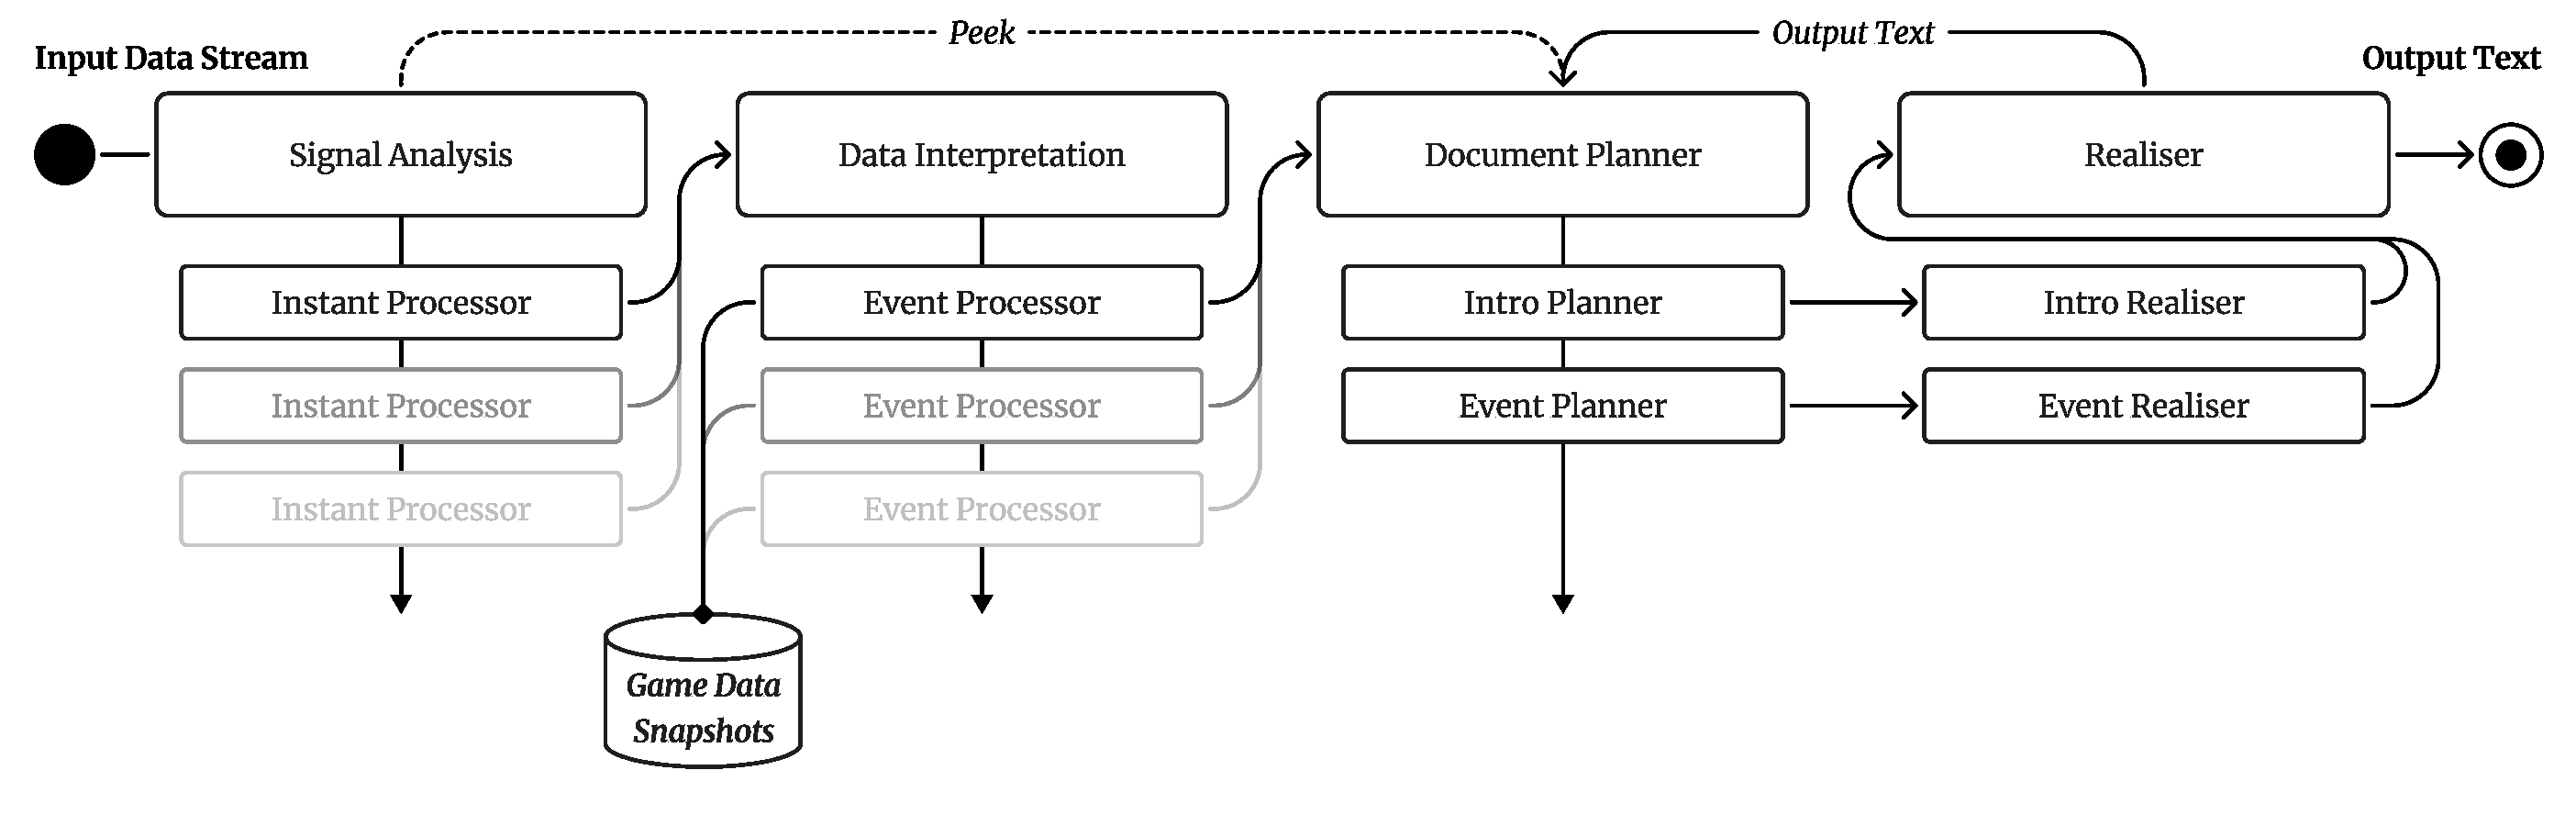
\includegraphics[width=\textwidth]{assets/pipeline-base.pdf}%
  }{%
    \fbox{\parbox{0.95\textwidth}{\centering Placeholder: missing file\\`assets/pipeline-base.pdf`}}%
  }
  \caption{High-level data flow of the \textit{SAGE} pipeline, enhanced with Age of Empires II-specific content selection and realization steps.} 
  \label{fig:pipeline-base}
\end{figure}
\begin{enumerate}
  \item Raw event data is ingested from the exported CaptureAge data in the Apache Arrow format.
  \item Events are processed through the Signal Analyzer, where they are filtered and clustered. Effectively events can be buffered until clusters are decided to be complete.
  \item Events are passed to the Data Interpreter for enrichment with contextual data from the corresponding game state snapshots.
  \item The Document Planner organizes enriched events into content units for realization. For this it can buffer events or peek at ongoing events to decide when to emit content units.
  \item Each content unit is realized into text by the LLM-based Realizer. The output is sent back to the Document Planner to allow it to provide future LLM calls with previously generated context. \footnote{Strictly speaking, we don't need to send it back, and keep it in the Realizer module, but since Document Planning and realization operate in pairs we prefer making the Realizer stateless.}
  \item Realized text segments are concatenated to form the final live text commentary.
\end{enumerate}

\section{Data Preparation}\label{sec:data-preparation}
\subsection{Recorded Games}
We retrieved recorded games with permission from King of the Desert IV\footnote{Permission kindly given by MembTV with assistance from DonDinardoni, who labeled each recorded game file for the set, players, and match numbers.}, the next installment of the tournament used in the preliminary study (Chapter~\ref{chap:viewer-study}), a year later. Recorded games--containing all player commands and starting state--were replayed in the version compatible \footnote{We used a community tool for that: \url{https://github.com/gregstein/DE-Replays-Manager/}} Age of Empires II: Definitive Edition client using an automated script via the in-game API to produce the CaptureAge data format.

\subsection{CaptureAge Data}
We extracted a subset of the recorded game data into the CaptureAge format, focusing on key events and player actions (Instants) and minute-long snapshots (60-second windows were found to have an acceptable file-size/retrieval-duration trade-off). Since Signal Analysis can buffer event data before context enrichment, the prototype needs access to previous game states to enrich events correctly. We therefore keep snapshot data as windowed state slices with incremental window identifiers (IDs) available for retrieval during interpretation; moving this state-tracking fully into ingestion may be preferable, at the cost of separation of concerns to be able to directly enrich during and avoid using out-dated state or caching large amounts of data. This also limits time-travel during enrichment: if interpretation happens later than event detection (due to buffering), we can still enrich using the snapshot that was current at the event time rather than whatever the latest state happens to be at interpretation time. However the 60-second window size may still introduce aliasing, where there never was a world state that exactly matches the event time. The dataset includes:
\begin{itemize}
  \item \textbf{Snapshot data:} Entities (units, buildings, resources), Masters (static data), Research States, Player States, and World data (time, prices).
  \item \textbf{Starting states:} Map terrain and settings (e.g., map name and dimensions; in our KotD IV dataset: Arabia, 120$\times$120 tiles).
  \item \textbf{Instants:} Entity events (e.g., created, died) and technology events.
  \item \textbf{Strings:} ID-to-text mapping.
\end{itemize}

The game lobby settings used for our recorded games are listed in Appendix~\ref{appendix:lobby-settings}. Selected snapshot data entries were annotated with metadata such as lifecycle changes (Created, Updated, Deleted, Transient --- came into and outof existence in the same window) and visibility timestamps to support debugging and event reporting. Each file is exported in the portable Apache Arrow format using Arquero \cite{arquero}, allowing for platform-agnostic efficient columnar storage and retrieval. All data is described in a descriptor schema containing the recorded game name, a list of files generated (one per type), and each file's window size and time boundaries, so window IDs can be mapped to game time\footnote{Game time is typically 1.69 times faster than real time.}. A full overview of the extracted data, including the schema and field definitions, can be found in Appendix~\ref{appendix:data-schema}.

\subsection{Dataset Scope and Release}
The evaluation corpus consists of 173 matches from King of the Desert IV, a top-level AoE2 tournament. Alongside it, we release a substantially larger dataset of 3,100 competitive matches, collected from competitive ranked 1v1 ladder matches in May 2026. Both datasets are exported at 1-second and 60-second snapshot resolutions. The full breadth of covered data types (including entities, player states, research states, command streams, world state, and significant derived events) is documented on the dataset page (Appendix~\ref{app:corpus}). To our knowledge, no comparable dataset exists at this level of continuous full-state telemetry for any esports title; prior work relies on sparse event logs or video feeds that do not expose structured game state directly.

\subsection{Iteration}
When iterating on the prototype, we focused on a specific configuration of the pipeline's rule-based stages (including event clustering thresholds, content prioritization rules, and narrative structure) to ensure we produced output suitable for evaluation. The following sections present the final results after this iteration. We occasionally mention other approaches we tested as well. The criteria used to assess progress and the outcomes are discussed in Section~\ref{sec:system-design-conclusion}.

Iteration is done on a single recorded game to allow for quick testing and validation. For this we chose a randomly selected game from our dataset, with a duration of approximately 45 in-game minutes, which is representative of typical match lengths. For this we picked match Group B - Round 1, Game 2 between Mbl and Vinchester from the King of the Desert IV tournament. This match features a balanced mix of battles, economy management, and strategic plays, making it suitable for testing the various modules and pipeline stages.

% \subsection{Iteration Outcomes}
% Above we described the implementation as it stands now. During the iteration process several changes were made to the design in order to reach the desired output quality and stability. Below we list some of the more significant changes:

% \begin{itemize}
%   \item We tried several different data structures and snapshot intervals. The data as described in Appendix~\ref{appendix:data-schema} contains unused data points that were retained to support iteration and potential future experiments.
%   \item We tested several different prompting techniques for the LLM-based Realizer (e.g., prompt variations, structures, few-shot vs. no-shot, alternative style descriptions) before settling on the current configuration.
%   \item We implemented and compared different detection strategies for battles and building events, as part of the original design, and pruned those that did not contribute clearly to summary quality.
%   \item We implemented an initial rule-based realization system for locations. This may be of interest as a cheap pre-realization step to support LLMs that work better with human-readable, linear text representations \cite{wang2024} instead of nested JSON structures.
%   \item We added additional data points to obtain the correct information as we developed the system (e.g., gameStatus was initially believed to contain resigned status to help indicate match endings, but this was not the case).
% \end{itemize}

\section{Pipeline Implementation}\label{sec:pipeline-implementation}
\subsection{Implementation Notes}
The prototype system for \textit{SAGE} is implemented in TypeScript, aligning with the CaptureAge tooling and allowing us to reuse existing data-processing utilities. Strong static typing helped us ensure that data is passed correctly between stages and modules, and helped highlight malformed or missing information early during development. To support this, we created a set of specialized generic types to ensure correct inference of the event types at each stage of the pipeline.
As such, the stack uses Node 22 with Yarn 4 and TypeScript 5.8. Overall, the stack is reasonably light: Arquero for reading and querying Apache Arrow, Zod for external data validation, and Remeda for functional programming utilities. We employ Jest as an iterative development aid for interactively running and debugging targeted code.

A full high-level visualization of the pipeline implementation can be found in Figure~\ref{fig:data-pipeline}.

\begin{figure}[htbp]
  \centering
  % Avoid build errors if file is missing
  \IfFileExists{assets/data-pipeline.pdf}{%
    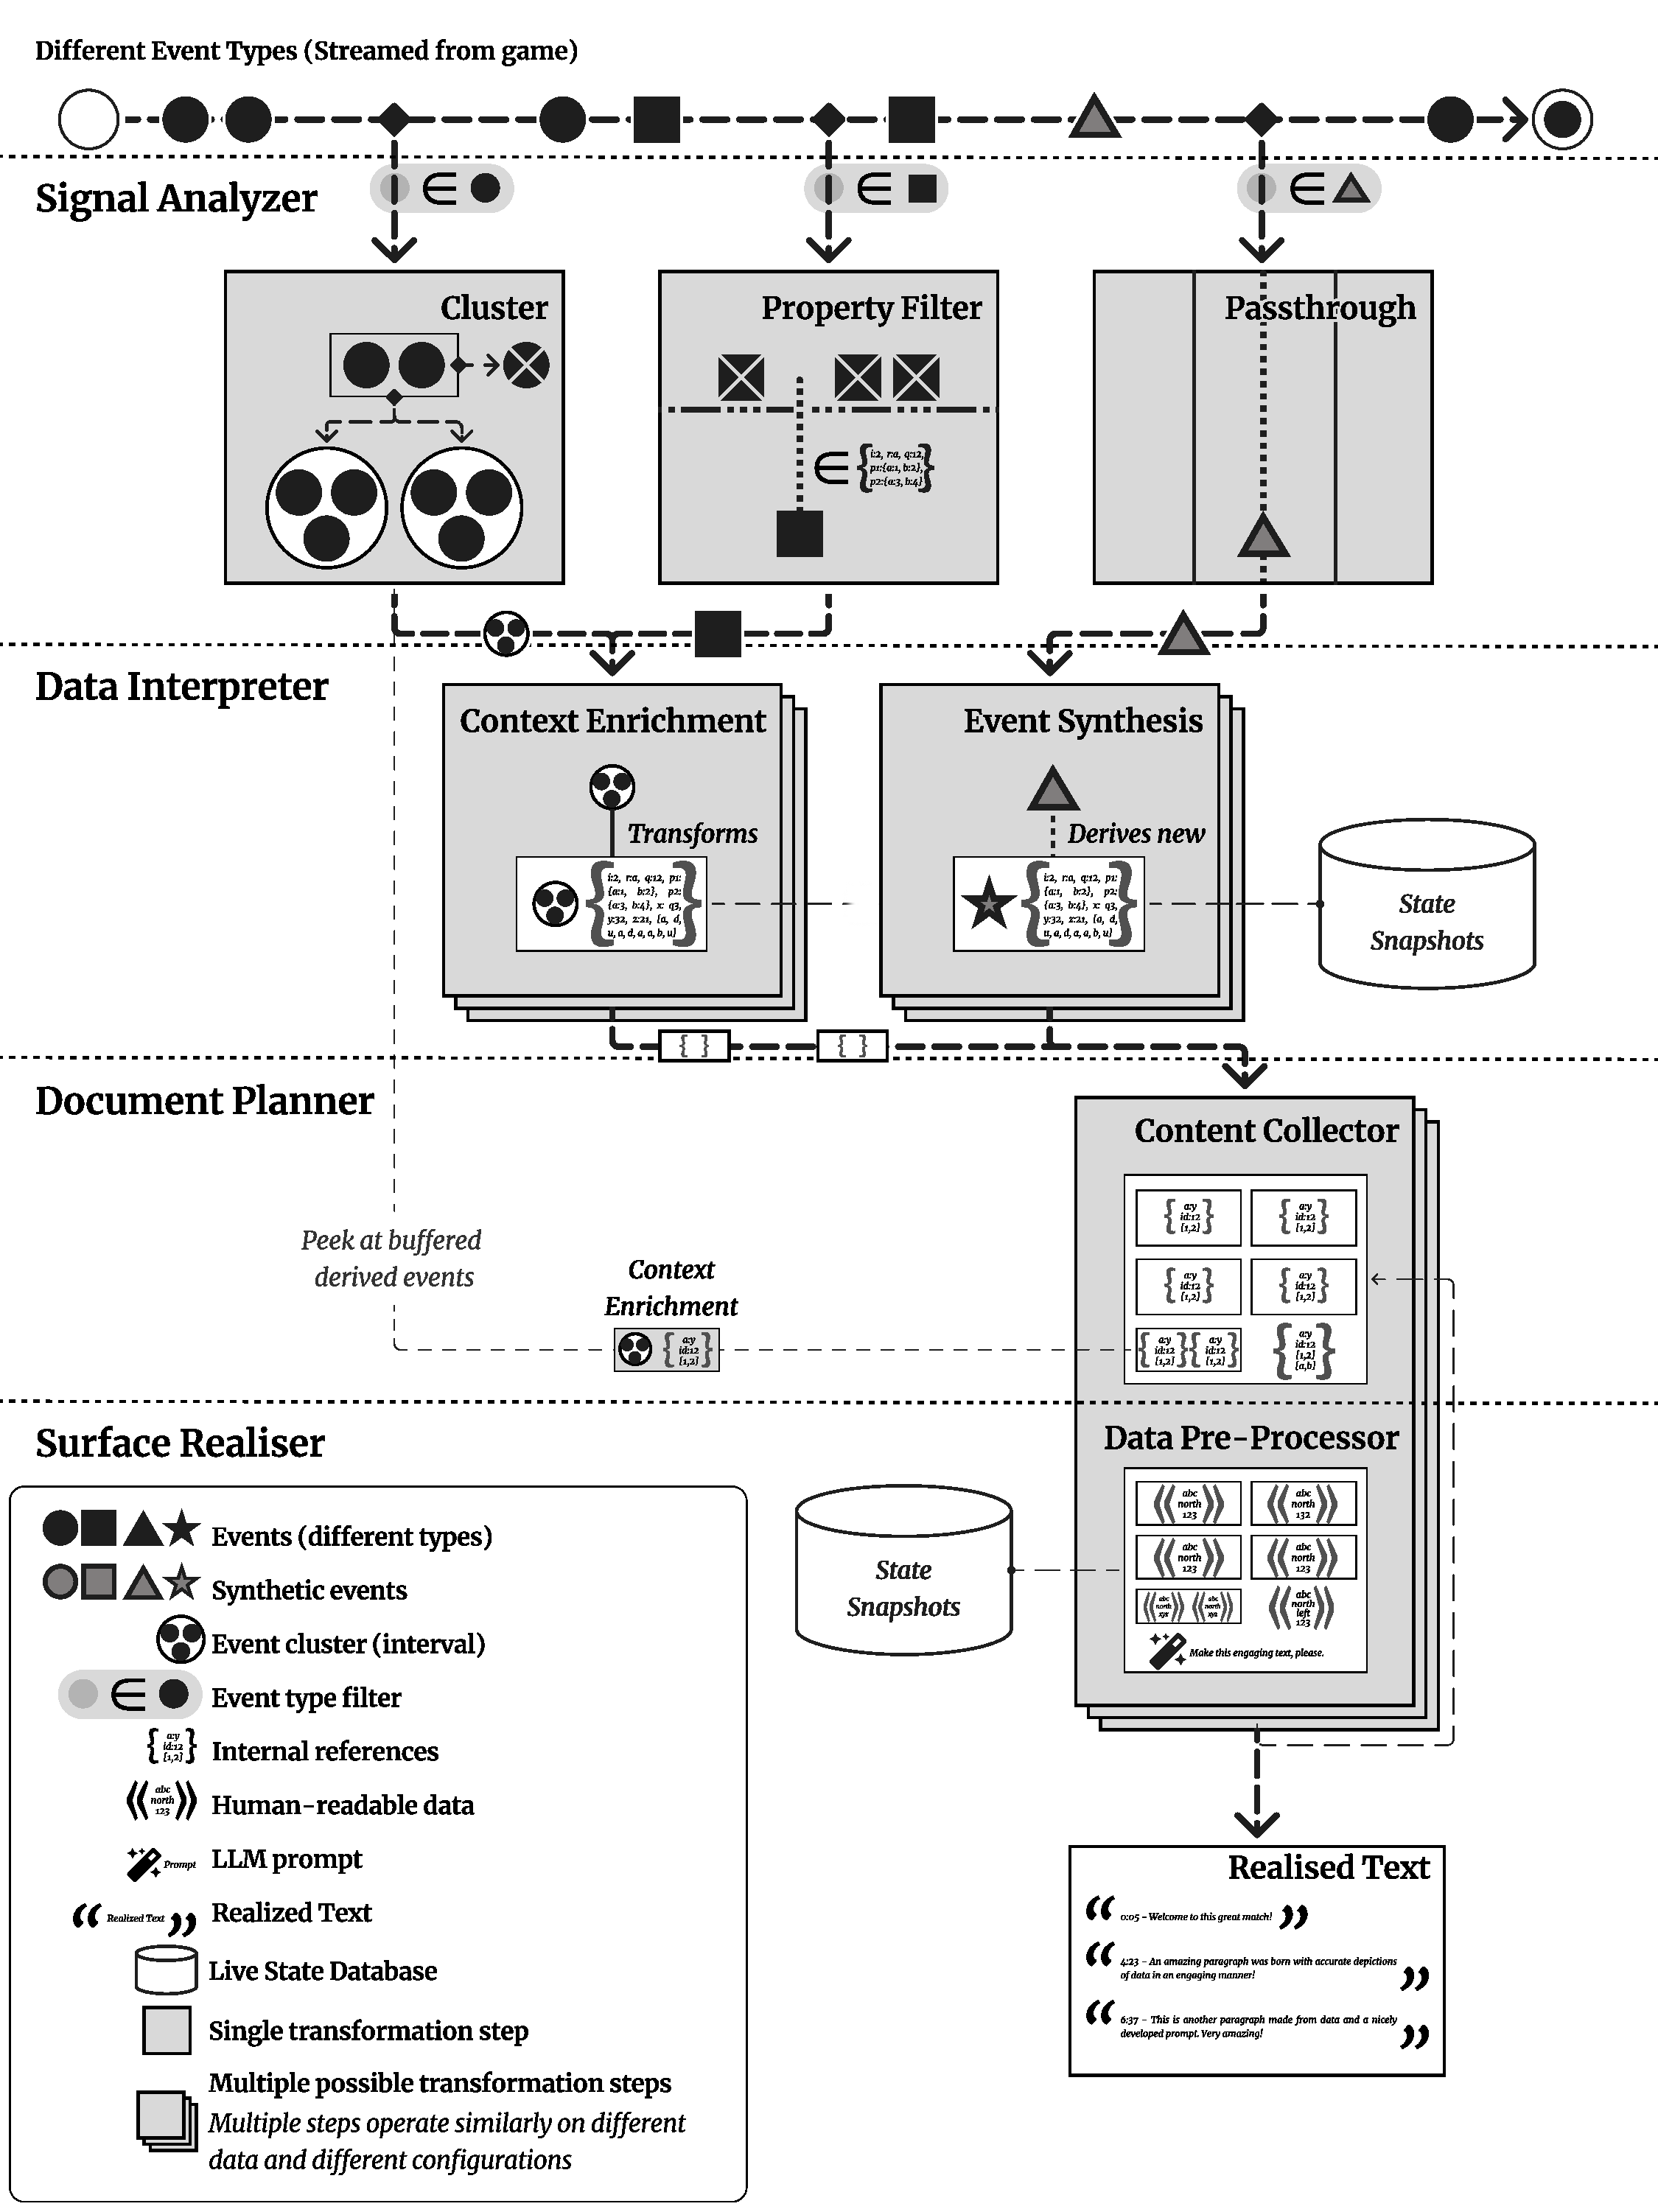
\includegraphics[width=\textwidth]{assets/data-pipeline.pdf}%
  }{%
    \fbox{\parbox{0.95\textwidth}{\centering Placeholder: missing file\\`assets/data-pipeline.pdf`}}%
  }
  \caption{Generalized overview of the \textit{SAGE} pipeline implementation, showing data flows between stages and steps. Each stage contains multiple steps; steps can have different configurations depending on the architectural module setup.}
  \label{fig:data-pipeline}

\end{figure}

The full code as well as a large dataset of CaptureAge games and generated summaries are available online \footnote{See Appendix~\ref{app:corpus} and Appendix~\ref{app:source-code} for corpus and source-code links}.

\subsection{Data Ingestion}
As a first step, we ingest the exported data from the CaptureAge API. We read the description file and load all files accordingly. The data is stored in a structure that allows for efficient retrieval of snapshot data based on time (windowId) using Arquero \cite{arquero}. It also allows for pre-filtering (e.g., to exclude thousands of entries for trees, arrows, and doppelganger entities to reduce query time) and caching for performance. We use the same structure as described in Appendix~\ref{appendix:data-schema}. In practice, we use relational queries to retrieve an initial data set and then do final filtering and processing in TypeScript. Relational queries are more efficient for large data sets, while TypeScript allows for more complex logic. An overview of what is exported from this stage can be found in Appendix~\ref{sec:example-ingestion}.

\subsection{Signal Analysis}
To mimic SAGE's online operation (processing event data incrementally as it arrives rather than from a complete batch), while using the exported dataset, we stream event data in chronological order, simulating real-time arrival. We intertwine this with a time event (Minute-Tick) every in-game minute as a heartbeat that may trigger specific time-based updates (e.g., introduction generation, or trigger a Planner flush), which also ensures that time-based buffers can be closed even when the event stream is otherwise quiet.

Signal Analysis is implemented as an event-type-specific inner pipeline: each step may emit zero or more derived events into the Signal Analysis output stream. Step configurations are defined by the architectural module setup; in our configurations, modules do not operate on overlapping event types, avoiding duplicate realization. Signal Analysis comprises two categories of steps:

\begin{itemize}
  \item \textbf{Spatiotemporal clustering:} Applied to events possessing both spatial and temporal attributes (e.g., damage events). This step groups events based on proximity in space and time, enabling identification of meaningful clusters such as fights or raids.
  \item \textbf{Property filtering:} Selects and passes only specific instants relevant to downstream processing (e.g., filtering for Castles and Town Centers among building events).
\end{itemize}

In practice, all modules use the same configuration for this stage: damage and death event clustering, building-type filtering, and passthrough for time ticks.

\subsubsection{Spatiotemporal Clustering}
Based on a comparison of spatiotemporal data clustering methods, we use a spatiotemporal variant of DBSCAN (ST-DBSCAN)\cite{shi2019, ansari2020} to cluster damage and kill events into fights based on temporal proximity and spatial location. This clustering step is the concrete implementation of the event abstraction layer, transforming the raw Instant damage events into Interval battle events. This method meets all requirements:

\begin{itemize}
  \item \textbf{Online (live) capability} - continuous clustering and ability to release clusters before processing the whole stream.
  \item \textbf{Arbitrary cluster count} - many battles can happen in parallel, and we don't want to assume a fixed number of clusters.
  \item \textbf{Arbitrary cluster shape} - we don't want to assume that battles are always spatially compact or temporally contiguous, as players may engage in hit-and-run tactics or spread out over time and space.
  \item \textbf{Arbitrary number of events per cluster} - we don't know how many events will be in a fight, and we want to capture both small skirmishes and large battles.
\end{itemize}

Input data is expected to be chronologically ordered. DBSCAN clusters data points if they are within range of at least a minimum number of other points (\texttt{minPts}) within a given radius (\texttt{eps}). This allows for two clusters to be merged if points of both are within range. This clustering allows us to identify sustained battles between players, which are critical for generating meaningful summaries.

A practical observation is that the temporal window combined with ordered input data allows for releasing clusters before the whole data stream has been processed, supporting the online capability requirement. In addition, we allow for peeking ongoing clusters and requesting them to be closed early if needed when downstream stages (Document Planner) require a summary of the current fight.

Figure~\ref{fig:online-temporal-spatial-clustering} provides an intuition for this online behavior: events arrive in chronological order, clusters can gain new events as they arrive, and clusters can be closed once no new events arrive within $\tau$ seconds.

\begin{figure}[htbp]
  \centering
  \IfFileExists{assets/online-temporal-spatial-clustering.pdf}{%
    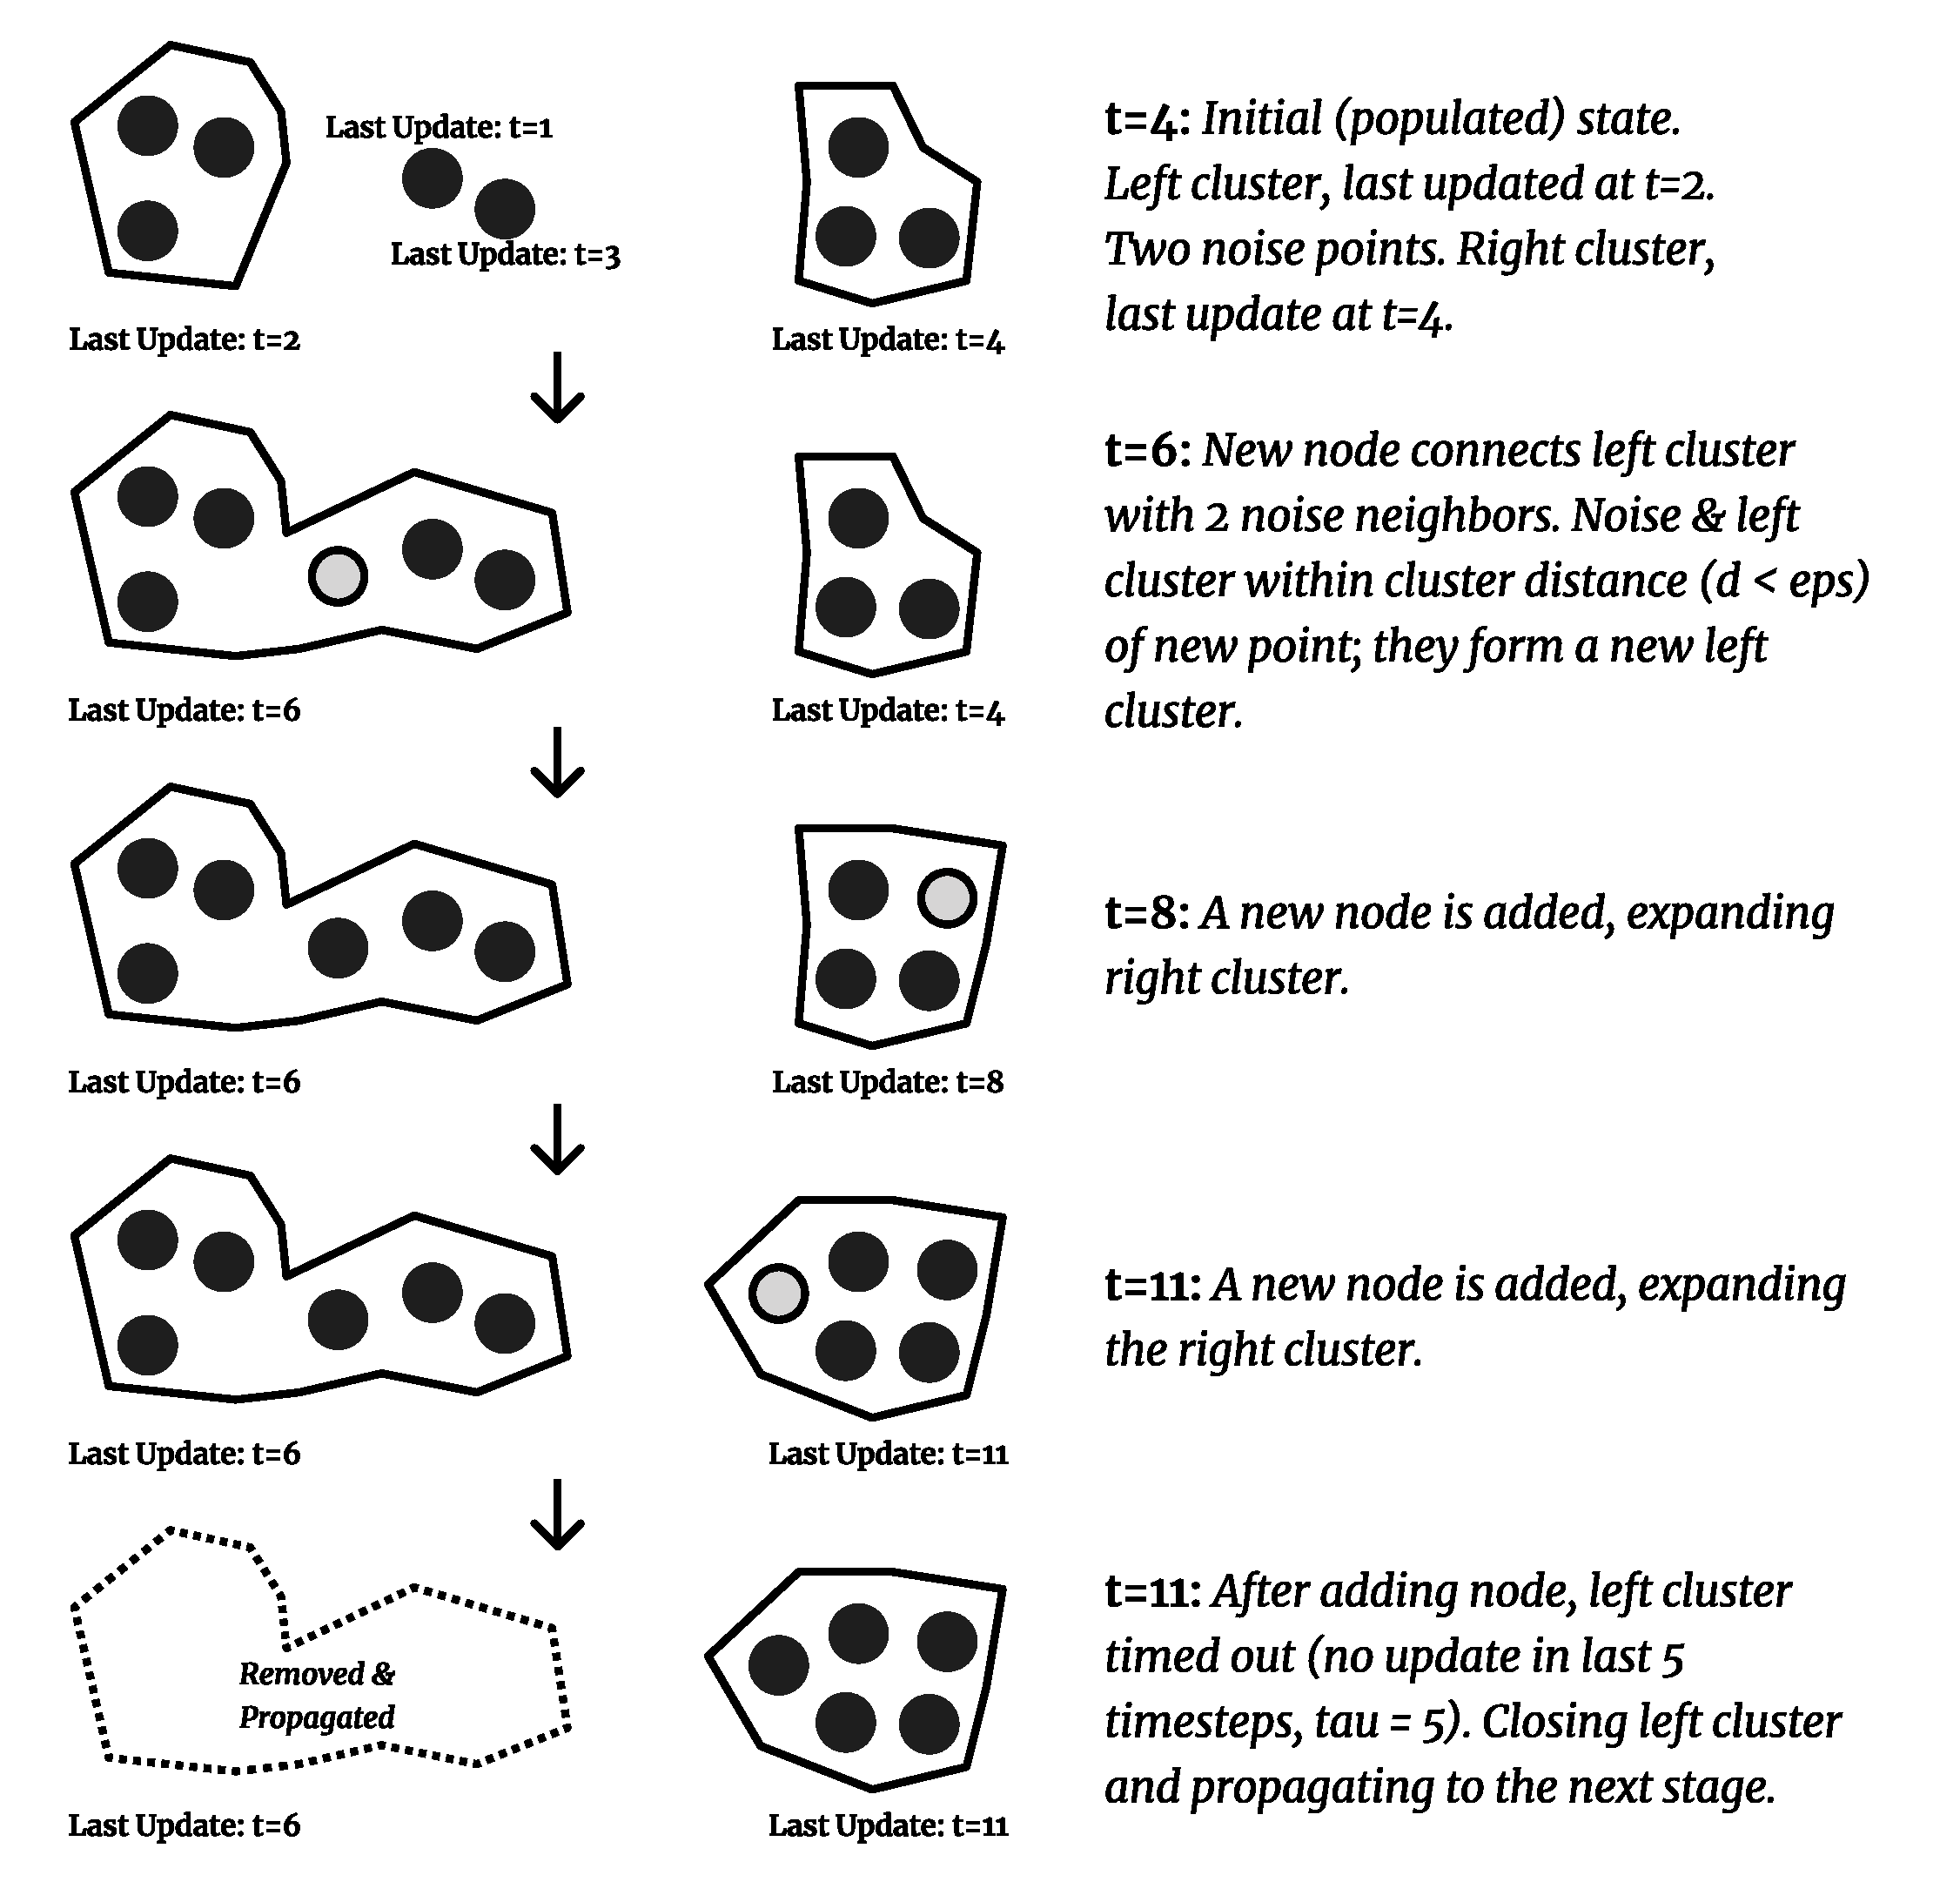
\includegraphics[width=\textwidth]{assets/online-temporal-spatial-clustering.pdf}%
  }{%
    \fbox{\parbox{0.95\textwidth}{\centering Placeholder: missing file\\`assets/online-temporal-spatial-clustering.pdf`}}%
  }
  \caption{Online temporal-spatial clustering example, showing how incoming events connect noise (t=5 through t=6), how existing clusters can gain new events (t=8 through t=11) and finally how old clusters are closed off (t=11, final). The grey circle indicates a newly arrived event.}
  \label{fig:online-temporal-spatial-clustering}
\end{figure}

Full pseudocode, implementation notes, and parameter values are provided in Appendix~\ref{appendix:signal-analysis-details}.

\subsubsection{Property Filtering}
We filter building construction events to include only narratively salient building types (Castles and Kreposts --- a "Slavs" alternative option to a Castle --- Town Centers, and Towers) to reduce noise and downstream processing load. This is implemented as a set of simple rule-based checks for entity type against a predefined list of building type IDs. While it may be interesting to explore linked construction processes (Building foundation placed, Construction started, Building completed), we leave this for future work.

\subsubsection{Minute-Tick Events}
Minute-Ticks are Synthetic Events added every in-game minute to serve as a heartbeat for periodic downstream updates (e.g., generating Introductions or flushing the Planner) and to ensure that time-based windows (e.g., temporal clustering timeouts) can still be evaluated during lulls. They are passed through to the next stage without modification; an overview of what is exported from this stage can be found in Appendix~\ref{sec:example-signal}.

\subsection{Data Interpretation}
Like Signal Analysis, Data Interpretation is implemented as an event-type-specific inner pipeline; each step can emit zero or more enriched events. This stage enriches derived (clustered) events with snapshot-based context such as location (e.g., relative to player bases), unit types, and owner data.
\subsubsection{Enrichment Steps}
We apply the following enrichment steps to each event, depending on the event type, largely aligned with the A-E-P+S framework and identified event cues from the domain analysis:

\begin{itemize}
  \item \textbf{Battles:}
    \begin{itemize}
      \item \textbf{Participants:} We identify the units involved in the battle, including their types and counts.
      \item \textbf{Casualties:} We track the units lost during the battle for each player.
      \item \textbf{Survivors:} We list the units remaining after the battle.
      \item \textbf{Army Composition:} We describe the overall composition of the armies involved (e.g., "mostly archers"). We also indicate the proportion of each unit type being in forward position.
      \item \textbf{Positional Context:} We add the named location of the battle (e.g., ``near red's forward gold'').
      \item \textbf{Economy State:} We include the current resource distribution and Villager counts.
      \item \textbf{Technology State:} We list relevant technologies researched or in progress.
    \end{itemize}
  \item \textbf{Construction:}
    \begin{itemize}
      \item \textbf{Forwardedness:} We identify for construction events whether the building is forward (closer to enemy base) or defensive (closer to own base), as this greatly influences the narrative importance of the event.
      \item \textbf{Positional Context:} We add the named location of the building (e.g., ``near red's forward gold'').
    \end{itemize}
\end{itemize}

\subsubsection{Event Categorization}
After context enrichment we categorize events into subtypes using a rule-based approach. For example, battles can be categorized into raids, full-scale battles, skirmishes, etc. based on the participants and casualties involved. This helps the Document Planner decide how to prioritize and structure the content (e.g., as \texttt{fightType} on battle events).

\subsubsection{Synthetic Events}
Based on Minute-Ticks we can also generate Synthetic Events that are not triggered by an instant-driven cue: introduction events at the start of the game, end-of-game detection, and (optionally) strategy detections (e.g., Drush --- an early Dark Age rush using Militia units --- or Scout Rush) based on the current units and buildings.

We don't add state info to construction events, since they don't typically influence the key game state metrics as much as battles do.

This stage corresponds to the Environment and Performance enrichment layers of the A-E-P+S framework. Specifically, we enrich events with Environmental information (civilization name, economy distribution, army composition, and positional context) and Performance metrics (technology states, military strength, and economic comparisons). Sensor-level data (visibility information capturing what each player can currently see through the Fog of War) is omitted for this study to reduce scope and file size, and the processing time that including per-player visibility snapshots would incur, with minimal situational impact.

For each event we can only access snapshot data for the current time tick, unless it was explicitly cached earlier, ensuring the online nature of the system. This means that enrichment must be computed incrementally and cannot rely on future game states.

A special case uses the first time-tick events to trigger introduction generation, based on the initial snapshot of the map and players.

\subsubsection{Map Positions}
To support comprehension in a text-only medium, we add stable named locations as macro-context anchors (e.g., ``red's forward gold''). This matches the finding from the user study (Chapter~\ref{chap:viewer-study}) that readers want map-position cues to connect isolated events to a coherent match state.
To report on map positions across events we query entity and terrain features using a classic spatial-only DBSCAN clustering algorithm at the start of the match. Based on the rules of Arabia (generally regarded as the most standard map for competitive play), which has standardized and consistent resources sizes and placements, we can reliably infer the location on the randomly generated map. We identify key map features such as Gold Mines, Woodlines and Sheep, as well as hills and ponds. We then give each of these a positional description relative to each player's starting location. We use three metrics for this: relative cardinal direction (N, NE, E, SE, etc.), distance (close, medium, far; crisp thresholds defined per resource), and forwardedness (a common way to describe the quality of a resource --- relative to the location of both players, implying how exposed it is to enemy attacks, we calculate an angle using a dot-product). Then we give these a name using a TypeScript port of the classic rule-based SimpleNLG Java library\cite{simpleNLG}. Compounding distance, direction, and forwardedness gives us descriptions such as ``Blue's forward, main stone mine''. We did this to obtain consistent naming between realizations, instead of relying on the LLM to generate these descriptions each time based on symbolic descriptions and coordinates. These are later used to anchor events spatially in the realization (``north-west'', or more descriptively ``neutral, north-east hill''.) While specifics are based on the Arabia map ruleset, the same approach can be applied to other maps with different resource placements and types.

We don't update the map layout as the game progresses, which is likely to happen (e.g. Gold Mines depleting or new forward expansions becoming the relevant anchor). Instead we focus on the starting state as a proof of concept. This may reduce the accuracy of later event descriptions as named anchors become stale, but generally the starting state is sufficient to ground most events.

\subsubsection{Map Introduction}
To synthesize the Map Introduction event we provide each player's name, cardinal starting location on the map and civilization. When the \textit{Expert Insights} module is enabled (see Section~\ref{sec:modules}), this introduction is further enriched with detailed civilization attributes and player playstyle information. This grounds the introduction in both the current game state and broader context: the players' identities and their civilizations' capabilities. An overview of what is exported from this stage can be found in Appendix~\ref{sec:example-interpretation}.

\subsection{Document Planning}
Document Planning receives enriched events from Data Interpretation and organizes them into content units for realization. The Planner uses event type, timeouts, and cooldown counters to (a) emit two introductions (Match Intro and Map Quality) immediately and (b) maintain a buffer of pending events. Battle and construction events are held until a periodic tick check meets one of three flush conditions: there are pending battles and their cooldown has expired, a 3-minute timeout has elapsed since the last flush, or an end-of-game event is present in the buffer.
To support live operation, the Planner can also peek at ongoing clusters in Signal Analysis when it needs a partial summary. Peeked events are explicitly marked as ongoing in the data passed to the Realizer to avoid reader confusion.

For the base module everything is passed on as it arrives, with no buffering, with the only ``event structuring'' activating for the final event to ensure that all ongoing battles are realized as well in the concluding section.

When the \textit{Event Structuring} module is active, the Planner employs a buffering strategy to identify and group related events before realization. This allows for the construction of composite events that capture parallel actions, rather than treating each event in isolation. Algorithm~\ref{alg:doc-planning} shows the core buffering and flush logic.

While Document Planning in its classical implementation is responsible for most content selection, here we forward part of this responsibility to the LLM-based Realizer. This gives the LLM more freedom to express the content in an engaging manner while still ensuring that the important content is included in the summary. An overview of what is exported from this stage can be found in Appendix~\ref{sec:example-planning}.

\subsection{Realization}
We use Gemini 2.5 Flash as the LLM-based Realizer for our system, via the Google Cloud API. The Realizer is called once per content unit generated by the Planner and returns a realized text segment.

We chose Gemini 2.5 Flash due to its low time-to-first-token latency, high throughput and large context window, in addition to high performance in ranking tasks \cite{gemini2025}. We used the June 2025 update. We configured the model with a fixed seed of 1 and a temperature of 1 for all realization calls; thinking mode was disabled. This matches the provider default temperature, and in our iterative testing it provided a workable balance between accurate reporting and engaging content. Since we were Realizing based on a predefined dataset (not live streaming data), we added additional timeouts between calls to avoid rate-limiting issues when realizing a large number of inputs in sequence.

The output of each realization call is sent back to the Document Planner to provide continuity in subsequent calls; realized segments are then concatenated to form the final summary.

\subsubsection{Context Design}
Each realization call uses a fixed system instruction that defines the model's role and constraints, plus call-specific user input. The system instruction always consists of the same parts:

\begin{itemize}
  \item \textbf{Base instruction:} Describes the LLM's role and constraints, including a specification of the input data format.
  \item \textbf{Output format:} No formatting of any kind (including Markdown and HTML) is permitted, to avoid markup artifacts and keep the output easy to present in plain-text interfaces
  \item \textbf{Output length:} Configurable word-count limit, allowing for under-generation.
  \item \textbf{Output language:} Always English.
\end{itemize}

Each content-unit type (Match Introduction, Map Introduction, Battle Events, Construction Event, Strategy Detection (Expert Insights)) from the Document Planner has a prompt associated with it with the following structure:
\begin{itemize}
  \item \textbf{Communicative goal:} Specifies what the text should express to the reader. This varies by realization type (e.g., introduction, event), but is consistent between each module.
  \item \textbf{Writing style:} Description of the desired writing style, we set the same always-enable architectural module for Writing Style here.
  \item \textbf{Additional notes:} Any further instructions for the LLM, including architectural model-specific guidance and explanations of any added data. If data is provided for this request, a prompt explains what is contained and where to find it.
\end{itemize}

For each specific realization call we then add:
\begin{itemize}
  \item \textbf{Input data:} The data to be realized, formatted as described in the Base Instruction and sent in the \texttt{``user''} role.
  \item \textbf{All previously realized text:} Added in the \texttt{``model''} role to provide context and continuity for the LLM.
\end{itemize}

Formatting influences model behavior; we provide realization inputs as JavaScript Object Notation (JSON) \cite{he2024}, which produced relatively factually correct output in our validation samples \cite{gemini2025}. We also preprocess the input data (next section) to reduce ambiguity and prompt size.

Providing previously realized text improves coherence and referential consistency, but consumes context-window budget for long matches. In practice, we found that using a large part of the context had a severely negative impact on the system's ability to use the provided factual data and to consistently follow instructions. While we originally planned to add few-shot examples, they led to worse performance in our iterative testing, and greatly reduced creativity in using contextually enriched information. Rather than balancing this with temperature, we focused on improving the other parts of the prompt, including small prompt-formatting cues to emphasize key constraints.The exact prompts (including all modules) can be found in Appendix~\ref{appendix:prompts}.

\subsubsection{Data Preprocessing}
We preprocess the data before realization to improve the LLM-based Realizer's understanding of the data and reduce mistakes. This appears \footnote{Validating this would be interesting, but is out of scope for this project.} to have two main benefits: the model is better at understanding human-readable names than numeric IDs, and compact representations reduce the tokens needed to express the same information.

Concretely, we replace opaque numeric identifiers with human-readable names (player, unit, and technology names, as well as named locations rather than \texttt{(x, y)} coordinates). For example, locations are expressed as named places (e.g., ``LoomRush's forward, tertiary Gold Mine''), which seemed to improve the model's understanding of spatial relationships in our iterative testing. While these steps could be done inside the Realizer, we apply them earlier to simplify debugging and avoid expensive multi-table join queries.

To reduce size and complexity, we also flatten repeated structures into count maps (e.g., \texttt{"food": 2, "wood": 1}). This is applied to unit and technology reports as well as battle and environment compositions (including forward-vs-total counts where needed for context). We also convert millisecond timestamps to the in-game colon format (e.g., \texttt{2:14:12}); while \texttt{1:03} is ambiguous, alternatives like \texttt{1h23m23s} reduced clarity for AoE2 readers, so we kept the colon format.

Values that can be represented as integers are not changed (e.g., \texttt{totalEcoUnits: 12}). We also updated some keys to better express their meaning (e.g., \texttt{player} to \texttt{ownerName}) for constructed buildings. An overview of what is exported from this stage can be found in Appendix~\ref{sec:example-preprocessing}.

\subsection{End-to-End Example}
To illustrate how data transforms through the pipeline, we trace a single battle event from raw ingestion to final text. This is a simplified example; actual data structures may contain additional fields, see Appendix~\ref{appendix:examples} for full details.

\paragraph{1. Ingestion}
The system receives a stream of raw ``damage'' and ``death'' events.
\begin{lstlisting}[language=JavaScript, basicstyle=\ttfamily\footnotesize]
  ...
{ type: "damage", worldX: 23, worldY: 98, worldTime: 123550, subjectEntity: 101, objectEntity: 202, ... }
{ type: "death", worldX: 23, worldY: 98, worldTime: 123550, subjectEntity: 101, objectEntity: 202, ... }
\end{lstlisting}

\paragraph{2. Signal Analysis}
ST-DBSCAN clusters these instants into a single ``battle'' interval.
\begin{lstlisting}[language=JavaScript, basicstyle=\ttfamily\footnotesize]
{
    type: "battle",
    startTimeMs: 123450,
    endTimeMs: 123550,
    data: [ ... ] // Array of clustered events
}
\end{lstlisting}

\paragraph{3. Data Interpretation}
The event is enriched with context (participants, location, economy) and classified.
\begin{lstlisting}[language=JavaScript, basicstyle=\ttfamily\footnotesize]
{
    type: "battle",
    location: "Red's forward Gold",
    player1: { participants: ["Archer", ...], casualties: ["Archer", ...] },
    player2: { participants: ["Skirmisher", ...], casualties: [] },
    fightType: "skirmish",
    ...
}
\end{lstlisting}

\paragraph{4. Document Planning}
The Planner selects this event for realization and structures it into a content unit.
\begin{lstlisting}[language=JavaScript, basicstyle=\ttfamily\footnotesize]
{
    type: "multipleEvents",
    startTimeMs: 123450,
    endTimeMs: 123550,
    battles: [ ... ], // The enriched battle object(s)
    previousRealisation: [ ... ] //  supplied as "model" messages
}
\end{lstlisting}

\paragraph{5. Realization}
The LLM generates the final commentary based on the content unit and prompts.
\begin{lstlisting}[language=JavaScript, basicstyle=\ttfamily\footnotesize]
  ``A skirmish breaks out at Red's forward gold! Red's Archers are caught out by Blue's Skirmishers, taking heavy losses.''
\end{lstlisting}

For a complete list of data structures at each stage, see Appendix~\ref{appendix:examples}.

\section{Limitations}
We acknowledge several limitations in our system design:
\begin{itemize}
  \item \textbf{Data scope:} We rely on CaptureAge's reconstructed state and Instant Events; any omissions or inaccuracies there propagate downstream. We also cannot realistically iterate quickly on the amount of data that is provided by CaptureAge, since it requires re-running games and re-processing them to get old data; to cope with this, we use large snapshot windows. This also allows us to request data from earlier in the game, which is useful because our pipeline buffers data when clustering events from the stream. In a true live setting this would not be possible; instead we would need to retrieve data as we receive the stream or cache it for forward use.
  \item \textbf{Event detection:} Our Signal Analysis uses heuristic rule-based clustering; complex patterns may be missed or misclassified. In Section~\ref{sec:pipeline-implementation} we describe the clustering method we selected and discuss its limitations, aiming to reduce misclassification and omission. Furthermore, we have primarily focussed on clustering battle-related events, with some "gaps" filled with construction events, and per-module additions. This was a targeted approach, but more events can make for a richer narrative. For the purposes of this research, we accept this limitation, since we are more interested in the effect of context enrichment and event structuring on engageability.
  \item \textbf{LLM realization:} While flexible, LLMs can produce inconsistent phrasing or factual errors; we mitigate this by providing factual data but cannot eliminate it entirely. Our approach of enriching the data with E-P+S data and the \textit{Expert Insights} module aims to reduce these errors by providing more context to the LLM, essentially using Retrieval-Augmented Generation, i.e., explicitly retrieving relevant facts from the game state and feeding them into the prompt \cite{lewis2020}. In our development, we found LLMs preferable to the rule-based Realizers we initially planned to use. In addition, LLMs implicitly encode vast amounts of domain knowledge, effectively serving as a soft ontology. While useful, this does mean that we have less control over the exact linguistic output compared to a rule-based Realizer; to counteract this, we use negative prompting to avoid unwanted phrases.
\end{itemize}
Knowing these limitations helps with implementation-level decisions and with defining realistic outcomes for the development phase.

\subsection{Evaluation Constraints}
Since we want to evaluate engageability, we need to be able to test different configurations of the system. The modular design allows us to swap out modules and ablate them to test their effect on engageability. This requires testing many different configurations, which can be time-consuming. In addition, the generated text needs to be of a length that is reasonable to read for participants in a user study. Since the number of modules has a multiplicative effect on the number of configurations, we limit ourselves to varying two modules (\textit{Expert Insights} and \textit{Event Structuring}), while keeping the Writing Style module always enabled in our study conditions to ensure a baseline level of engageability. We also aim to shorten the generated text by limiting the maximum output length of each text in the Realizer, as well as removing less important events in the Document Planning stage and not reporting on lulls. This breaks with \citet{lewandowski2012}'s definition of minute-by-minute reports, where sometimes non-descriptive information is reported to fill lulls. We accept this limitation because we want to focus on engageability through descriptive information and event-driven reporting.

\section{Architectural Modules}
\label{sec:modules}

We aim to evaluate different strategies for enriching the generated text, based on our findings in the previous chapter and our aim to increase engageability. In particular, we want to test the effect of adding contextual information and how to deal with parallel events and their relations. \citet{callaway2002} propose an ablative design using architectural modules, where modules can be swapped or ablated to test different strategies for enriching the generated text. We follow a similar approach, introducing modules that can influence any stage of the pipeline by adding steps. This allows us to experiment with different enrichment strategies without altering the core pipeline.

\begin{figure}[htbp]
  \centering
  % Avoid build errors if file is missing
  \IfFileExists{assets/pipeline-modules.pdf}{%
    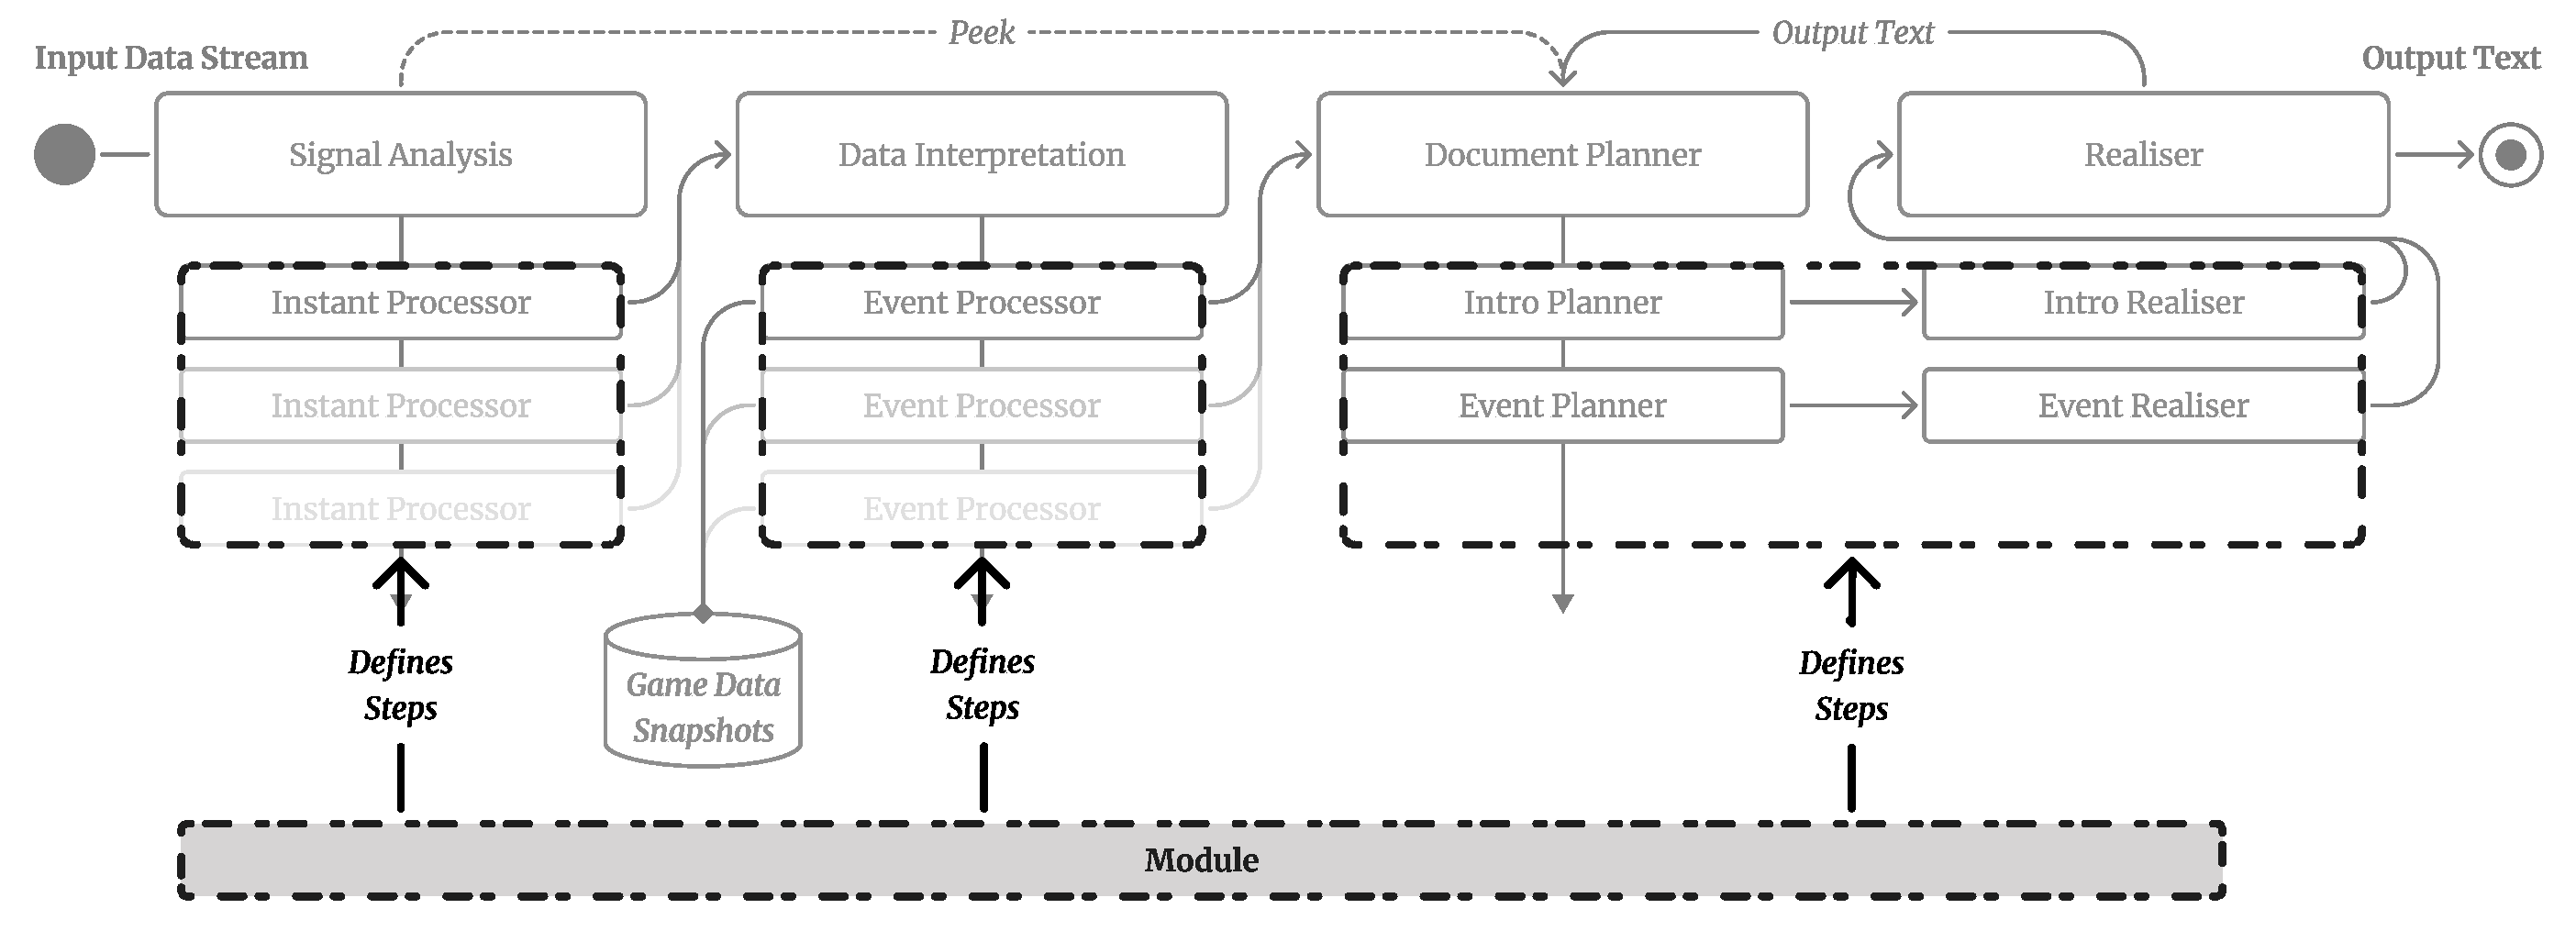
\includegraphics[width=\textwidth]{assets/pipeline-modules.pdf}%
  }{%
    \fbox{\parbox{0.95\textwidth}{\centering Placeholder: missing file\\`assets/pipeline-modules.pdf`}}%
  }
  \caption{Modules that can be independently enabled or disabled to test different strategies for enrichment of the generated text. A module can influence any stage of the pipeline by adding steps.}
  \label{fig:pipeline-modules}
\end{figure}

We test three engageability-related strategies by enabling and disabling modules independently:
\begin{enumerate}
  \item \textbf{Adding contextual information:} This is often provided by (color) commentators in live sports commentary. Although previous research has not directly validated its effect, it is frequently mentioned as an important factor \cite{li2020, margetis2023}.
  \item \textbf{Explaining parallel events:} Providing explanations for parallel events supports better understanding of the game state, as suggested by related work \cite{cheung2011starcraft} and anecdotal evidence from shoutcasters in our own analysis.
  \item \textbf{Stylistic variation:} Testing the effect of stylistic variation on engagement, as highlighted by analysis \cite{lewandowski2012, byro2017, gustin2020}, to see if mimicking the engaging style of esports shoutcasters improves reader engagement.
\end{enumerate}

We introduce three top-level architectural modules. Their inclusion is driven by experimentation goals rather than necessity for basic functionality. Each module can add steps in Signal Analysis, Data Interpretation, Document Planning, and Realization. Since modules can work together we ensure that any added step consumes data made available by upstream stages and produces outputs that remain compatible with downstream stages. In particular, Document Planning and Realization operate in pairs, so that each Planner output type has a corresponding Realizer configuration that produces a single realization for each content unit.

Figure~\ref{fig:pipeline-modules} illustrates how modules can influence any stage of the pipeline by adding steps. In our evaluation we vary \textit{Expert Insights} and \textit{Event Structuring}, while keeping the Writing Style module enabled to ensure a baseline level of engageability (see Evaluation Constraints above).

\subsection{Event Structuring}
The optional \textit{Event Structuring} module operates primarily at the Document Planning stage but influences the entire pipeline. Its main responsibility is to select the most important events, group them into coherent sequences, and provide a better trade-off between supportive context and events. This should be done in a way that supports reader understanding of complex, simultaneous actions.

\subsubsection{Document Planning}
The \textit{Event Structuring} module operates on the Planner's buffering mechanism. Instead of passing events immediately to the Realization stage, the Planner buffers events to identify temporal and spatial overlaps. Specifically, the prototype uses a buffer of at most 180 game seconds or 5 events. Within these buffers, events are sorted by importance (e.g., prioritizing large battles or those with significant economic damage over small skirmishes) to determine the narrative focus. It also ``peeks'' at the Signal Analysis stage to check for ongoing events that might be relevant to the current buffer, ensuring that related events are not split across different realization cycles.

\subsubsection{Realization}
When the \textit{Event Structuring} module is active, the Realizer receives grouped events instead of individual ones. The prompts are adjusted to instruct the LLM to weave these events into a single narrative segment (see Appendix~\ref{appendix:arch-modules-prompts}). This includes guidance on how to handle temporal overlaps and spatial relationships, ensuring that the summary reflects the complexity of simultaneous actions. With this, the Realizer is responsible for deciding both what information to include and which events to report on. We also reduced the number of updates. After experimentation, we gave it an additional 50\% word budget to still aim for the same document length range (500--800 words). Since the Document Planner decides how to group events, the Realizer can be consistent with the word budget per content-unit, to help focus on the most important events.

Following our previous observations, we prompted the LLM to emphasize Information Asymmetry for increased engagement. It was also told to clearly indicate when multiple events are happening at the same time using temporal Cues in the longer paragraphs, and the use of ``Transitional'' phrases such as ``Meanwhile, on the other side'', ``But their opponent doesn't know'', or ``What are they planning?'' to help readers follow the concurrent actions.

\subsubsection{Experiment: Agentic Document Planning}
We attempted a single, simple agentic approach as well, where the LLM was given a prompt to alternatively return a keyword (``<DEFER>'') to postpone realization to gather more events. It was given the task to reduce reporting on an Age (technology) progression basis (i.e., every minute before Castle Age, every 3 minutes after Castle Age). It was given the aim to use this mechanic to keep readers engaged. However, in our tests, it only postponed realization on a few occasions, ignoring the explicit frequency instructions to do so.

\subsection{Expert Insights}
The optional Expert Insights module enriches the raw game data with domain-specific knowledge, connecting observable facts to their strategic significance. This enrichment occurs primarily during the Data Interpretation stage. There we rely on two mechanisms: newly derived Synthetic Events and context enrichment of existing events. We also provide causality information (e.g., ``against early Archer attacks, defenses need to stretch a larger area to counter their arrow's range'') in the prompts for the LLM-based Realizer to leverage this information effectively. These prompts include data descriptions and minor points to allow it to better use the data and understand the implications.
Domain Knowledge is provided in Data Interpretation, while Analytical Knowledge is provided in the Realization stage.

\begin{itemize}
  \item \textbf{Player Data:} Adds context about the players, such as their known playstyles (e.g., ``aggressive'', ``defensive'') and historical performance. This data was retrieved from a static knowledge base compiled from community resource Liquipedia~\cite{liquipedia} and the author's knowledge. It includes details such as player names, clan affiliations, and typical strategic tendencies. Since players were anonymized in our user study, we include this background primarily to support reader understanding and to test whether prior player knowledge affects ``delight'' \cite{oshimi2015}.
  \item \textbf{Civilization Data:} Injects information about the civilizations played, including their unique strengths, weaknesses, and key units. This information, sourced from the Age of Empires II Fandom Wiki~\cite{aoe2wiki}, helps to explain \textit{why} certain events might be happening (e.g., a civilization's economic bonus enabling a faster advance). This injection is done for all battle events, since civilization traits often influence combat outcomes.
  \item \textbf{Strategy Detection:} Uses a fuzzy logic filter to detect high-level strategies (e.g., ``Tower Rush'', ``Fast Castle'') based on the distribution of units, buildings, and technologies. This allows the system to label a collection of events with a strategic intent. The Data Interpretation stage emits detected strategies as derived Synthetic Events, on a per Minute-Tick basis.
\end{itemize}

\subsubsection{Fuzzy Strategy Detection}
The strategy detection mechanism is implemented using a simple fuzzy logic engine that evaluates the game state against a set of predefined strategy templates. This approach allows for the detection of strategies that are not strictly binary but rather exist on an interval of confidence. In essence: ``If you see 2 archers we are likely seeing an archer rush, but if you see 5 archers we are certain''. These statements can be chained and combined: ``However, this strategy usually only occurs before 12 minutes and never after 15 minutes.'' There are many strategies in Age of Empires II, each with its own set of indicators which are also used by human commentators and players to identify them. Fuzzy sets are a methodology to combine these indicators into a single confidence score.

This system may deserve a full section, but it only contributes as a small part of an architectural module, so we provide a concise overview here; an example configuration is provided in Appendix~\ref{appendix:fuzzy-logic}.

\paragraph{Evaluation Input Fields}
Each strategy template defines a set of criteria based on the following input fields:
\begin{itemize}
  \item \textbf{Unit Criteria:} Evaluates the count and position of specific unit types. For example, a ``Tower Rush'' strategy might require a high number of Villagers in a forward position.
  \item \textbf{Building Criteria:} Similar to unit criteria, but for buildings. It checks for the presence, count, and position (forward vs. defensive) of key structures.
  \item \textbf{Technology Criteria:} Checks the state of specific technologies (researched, researching, or queued). This matters for timing-based strategies like ``Fast Castle''.
  \item \textbf{Villager Distribution:} Analyzes the economic focus of a player by evaluating the number of Villagers gathering specific resources (e.g., high stone allocation for a Tower Rush).
  \item \textbf{Constraints:} Hard constraints such as the current Age or Civilization, which act as binary filters.
\end{itemize}

\paragraph{Scoring and Combination}
Each criterion is evaluated using trapezoidal fuzzy sets, which map a numerical input (e.g., unit count) to a membership value between 0 and 1. Typically, these sets allow for a linear transition of confidence. For example, if we see 3 Militia, we might be 100\% confident that the ``Enough Militia Present'' criterion is met for ``Drush'' strategy, while 0 Militia gives 0\% confidence, and 1-2 Militia yields a value between 0-100\%.

However, we also employ these sets to enforce crisp requirements. By defining a trapezoid with a vertical ``cliff'' (e.g., using the \texttt{atLeast(n)} helper), we can create hard constraints where any value below $n$ has 0 membership and $n$ or above has 1. This allows the fuzzy logic system to handle binary conditions (like ``Must have Loom researched'' or ``Must have at least 2 Villagers on Stone'') alongside graded ones.

These individual membership values are then combined to form an overall confidence score for the strategy.

\begin{itemize}
  \item \textbf{Input Field Evaluation:} Each input field uses fuzzy sets defined by parameters like `atLeast`, `atMost`, or `between` to determine how well the current state matches the expected value.
  \item \textbf{Combination Logic:} Individual field scores are combined using standard fuzzy logic operators. Typically, criteria within a category are combined using a fuzzy AND (the minimum of all scores is propagated), while different categories can be weighted or combined to form the final score.
\end{itemize}

\paragraph{Runtime Execution}
In practice, the system iterates over all defined strategy templates for each Minute-Tick event.
\begin{enumerate}
  \item \textbf{Time Window Check:} First, the system checks if the current game time falls within the valid time window for the strategy (e.g., a ``Dark Age Rush'' is only valid in the early game).
  \item \textbf{State Evaluation:} If the time window is valid, the engine evaluates the current game state against the template's criteria to compute a confidence score.
  \item \textbf{Thresholding \& Selection:} Strategies with a confidence score below a minimum threshold (set to 0.3) are discarded. Among the remaining candidates, the strategy with the highest confidence score is selected and emitted as a Synthetic Event to the Data Interpretation stage.
\end{enumerate}

\paragraph{Strategy Template Generation}
The templates were created by an LLM (Gemini 2.5 Pro, version June 2025 (VSCode Copilot)), based on a list of strategies to detect and an overview of each leverage point (units, buildings, technologies, villager distribution). No additional information was given to the LLM about how these strategies manifest in-game, relying on the LLM's knowledge to create the initial templates. These were then manually reviewed and adjusted to ensure correctness and feasibility.

This is an interesting finding in itself, as it shows that LLMs can be used to generate domain-specific knowledge representations that can then be operationalized in a (much more computationally efficient, accessible and explainable) rule-based system, without prior training.

\subsubsection{Data Interpretation}
Based on the event type, the Expert Insights module enriches events with additional data: Match Introduction events are enriched with player and civilization data, Battle events are enriched with civilization data, and Synthetic Strategy Events are emitted as detected.

\subsubsection{Document Planning}
The \textit{Expert Insights} module modifies the Document Planner for strategy reporting. When a strategy is detected, it's always prioritized, ensuring that it's realized as soon as possible. The detected strategy is included in the context for all subsequent realizations, allowing the LLM to reference it when describing events. For this the Document Planner memorizes the last detected strategy for each player, and the time it was detected.

\subsubsection{Realization}
Each Realizer is told exactly where to find the additional \textit{Expert Insights} data and how it is structured. We provide instructions on how to interpret the data given several Analytical Knowledge examples (see Appendix~\ref{appendix:arch-modules-prompts}). This includes explanations of civilization strengths and weaknesses. For example if Gold is forward and your opponent is likely to make Archers (e.g., the Britons civilization), then wider walls or even a tower may be advisable. We include a small number of high level examples, explicitly pre-conditions and the possible implications, to help the LLM understand how to combine these data points effectively.

\paragraph{Negative Prompt}
Despite a general prompt asking the LLM to ground all its output in provided information and facts, it would still attempt to provide expert knowledge. To combat this, we explicitly added a negative prompt as a Realization-only module. This reduces the risk that, when no \textit{Expert Insights} data was provided, the LLM would hallucinate such information (or, in some cases, correctly infer it). This was tailored to each event type (e.g., for the Match Introduction it was given: ``Report only facts from the provided data - avoid general game knowledge.'').

\subsection{Writing Style}
The Style module is a stylistic configuration that operates at the Realization stage. Unlike the other modules, it does not alter the data flow or structure but adds a small prompt influencing how content is expressed.

We based this on the findings by \citet{lewandowski2012} on how to shape our target register of live text commentary (or online sports commentary, OSC). In particular the simple present use, copula be deletion, and use of spatial and temporal anchoring.

Initially we also requested the use of metaphorical language \cite{byro2017, gustin2020}, but the LLM was not able to apply this in a way that the author felt was in line with community expectations, so we removed this aspect. Instead we used simpler language to prompt engaging language.

\subsubsection{Realization Stage}
The Writing Style module only had a Realization-stage-specific influence, adding a simple prompt (detailed in Appendix~\ref{appendix:prompts}):
``Use dynamic, exciting language sparingly to maintain engagement while keeping content concise. Most content should be written in the simple present tense, feel free to use copula be deletion where appropriate.'' as the Writing Style component of the prompt.

This directly reflects the main findings, while encouraging the LLM to balance engagement with factual reporting.

An example sentence generated with this module active is:
\begin{quote}
  \textit{37:24 - A brutal major battle near red's Town Center! Blue's army is decimated, losing 27 units, while red loses only 14, mostly Villagers. Red still holds a strong military advantage!}
\end{quote}

This clearly shows copula be deletion (``\underline{There is} a brutal major battle...''), with most of the sentences written in the simple present tense, as well as the use of dynamic adjectives (``brutal'', ``decimated'') to increase engagement.

We procedurally added the timestamp to improve consistency across realizations, which the LLM struggled with. In general, it was able to add the positional data (near red's Town Center). \footnote{It's interesting that it was this good at supplying positional data, compared to adding consistent timestamps. This may be due to the fact that positional data is more semantically relevant to the event, while timestamps are more of a meta-data aspect, thus not being prioritized by the LLM.}

\section{Conclusion}\label{sec:system-design-conclusion}
The prototype delivers a modular, incremental pipeline that meets our feasibility goals: factual summaries based on high-fidelity game data, a clear structure aligned with our narrative design focusing on engageability, and extensibility through architectural modules.

\subsection{Discussion}
During prototype development, we adhered to five main criteria to ensure progress toward a functional system, and evaluated these criteria iteratively on a single representative match based on the author's judgment and checking the completeness at key points in the match (e.g., after the first big battle, after the first Castle Age, etc.):
\begin{itemize}
  \item \textbf{Structural Completeness:} Structural completeness was realized through deterministic Document Planning, ensuring that all key narrative components (introductions, battles, constructions) were represented in the final summary.
  \item \textbf{Data Correctness:} This is the most critical criterion, as the system's credibility hinges on accurate reporting, while rule-based event detection is limited in its accuracy. We validated correctness through manual review of generated summaries against the original game data and video-based shoutcasts, aiming to confirm that reported events and statistics matched in-game occurrences. It's not feasible to do this for every summary generated during iteration. However, the final evaluation did not reveal surface-level issues, and a preliminary run of four additional games (used for the evaluation in Chapter~\ref{chap:eval}) also did not surface obvious correctness problems.
  \item \textbf{Reporting Density:} Balancing the frequency of reported events was important. We found that the base case, realizing every event required a reduced target number of words per event to avoid overly long summaries. The \textit{Event Structuring} module helped improve this by grouping related events, allowing for richer context without overwhelming the reader, generally creating shorter summaries.
  \item \textbf{Readability:} We rarely found readability issues during iterative testing, mostly related to the LLM's output. From time to time a repeated sequence was found, which can be mitigated by tweaking the temperature, but we found this not frequent enough to warrant straying from the default recommended temperature. While we cannot say that the text is engaging without a formal evaluation, the output includes many of the stylistic elements we aimed for, such as simple present tense and copula be deletion, as well as spatial and temporal anchoring, while using dynamic language to increase engagement. It should be noted that the LLM sometimes realized text in other tenses, but this is technically permitted by the prompt, in line with prior findings \cite{lewandowski2012}. Informal feedback from other readers indicated that the summaries were easy to read and follow, with a coherent narrative flow, reducing a potential need to add a static visual modality for grounding the text.
  \item \textbf{Module Functionality:} Each architectural module was tested in isolation to confirm it contributed to the overall system. Since there is a clear interaction between \textit{Event Structuring} and the output (it increases the number of words per output section), we tested each module's interaction with \textit{Event Structuring} as well. In our tests, all modules behaved as expected.
\end{itemize}

These criteria served as effective guardrails, allowing us to iterate rapidly on a single representative match before scaling up.

However, we have not evaluated the system beyond a limited data set due to the scope of this thesis. This limitation is amplified by the non-deterministic nature of LLMs, where even small data differences can yield vastly different outcomes. A particular risk lies in the generalizability of detection steps—specifically fuzzy strategy detection (any parameter) and clustering sensitivity (\texttt{eps}, \texttt{minPts} and \texttt{tau}) — to different game scenarios and player styles. Fortunately, the modular architecture allows these components to be swapped for robust implementations in future work.

\subsection{Future Work}
Several areas for improvement emerged during development, particularly regarding the LLM's context window and data handling. We observed that some instructions in prompts, particularly stylistic and formatting directives, were ignored over time in longer matches, likely due to the prompt size (the data in particular) being large, causing context overflow. Future iterations could implement ``differential snapshots''—focusing on state changes rather than full data dumps—to reduce token usage and highlight standout changes. Agentic approaches could go further by making retrieval goal-driven: the system could decide what to retrieve for a given communicative goal (e.g., emphasize spectacle in a decisive fight, but emphasize strategic context or expert insight during lulls), and avoid enriching with facts that are not currently useful for realization. However, this shifts work into iterative retrieval and may increase response time without careful caching/prefetch strategies.

Reducing prompt size is also important for economic viability. In our current prototype configuration, realizing a full match can cost on the order of \$0.10 in API usage (driven largely by the amount of structured data passed into the Realizer), which makes full-match generation hard to justify in many real-world settings without more aggressive compression.

The current focus on start and end states of battles, while useful for visualization, can occasionally lead to repetitive narratives. Future work should explore ways to better capture the dynamic flow of combat. This can be done by passing the exact battle logs, or by implementing more sophisticated event detection that captures key turning points within battles.
Furthermore, while our early enrichment strategy is conceptually strong, it risks time misalignment due to the minute long windows, and looking up the data at Interpretation time, instead of at data ingestion time. In a live system, this means either enriching eagerly (at ingestion time) or preserving immutable snapshot views keyed to event/ingestion time, so later planning and realization cannot accidentally enriching against a ``newer'' (and therefore untruthful-for-that-moment) state. Adopting more advanced statistical methods or specialized models for state tracking—moving away from purely LLM-based enrichment—could improve practicality.

Requesting the LLM to generate a structured representation of the content before realization could also improve factual accuracy, as it would force the model to explicitly outline the information it plans to include. This intermediate step could be validated against the input data, reducing hallucinations, and would provide a clearer audit trail for the generated content.

Finally, the system's modularity opens the door for a generalized approach. By defining game-specific Signal Analysis and Data Interpretation modules, the core Realization and Planning components could be reused across different esports or even other time series data reporting domains.

The prototype is modular, incremental, and meets its feasibility goals: factual summaries from high-fidelity data, a structure aligned with the narrative design, and extensibility through architectural modules. Whether this design effectively improves engagement, and holds up in a less controlled environment is evaluated in the next chapter (Chapter~\ref{chap:eval}).
\chapter{Evaluation}\label{chap:eval}
This chapter evaluates generated match-update texts for Age of Empires II (AoE2). We assess linguistic quality and viewer engageability to guide future audio-visual summaries. Using a glass-box evaluation, we test the effects of two architectural modules (\textit{Expert Insights} and \textit{Event Structuring}) and analyze module effects using Linear Mixed Models (LMMs). Since the goal here is to evaluate the system, compared to the exploratory user study in Chapter~\ref{chap:viewer-study}, this evaluation uses a stricter checklist and additional diagnostics.

\section{Introduction}
Because we lack reference texts and aim to measure viewer-centered qualities such as engageability, we rely on human evaluation (see Chapter~\ref{chap:related}). Following \citet{wang2025}, we omit automated metrics like BLEU \cite{papineni2002}. These do not capture strategic commentary, do not measure engageability, and we lack comparative data for this modality. We therefore assess linguistic quality and the ability to engage viewers, in line with best practices \cite{vanderlee2021}.

Following our argument in Chapter~\ref{chap:related} (Section~\ref{sec:mses-motivations}), that engageability can be measured by how well a system matches viewer motivations, we adopt the ten Motivation Scale of Esports Spectatorship (MSES) motivations \cite{qian2020} as our lens, and refer to a system's ability to satisfy them as its \textit{engageability}.

We evaluate two architectural modules designed to improve engageability:
\begin{itemize}[noitemsep,topsep=0pt]
  \item \textbf{Expert Insights:} Adds context and analysis beyond raw events to clarify the significance of key moments, aiming to satisfy \textit{Skill Improvement}, \textit{Skill Appreciation}, and \textit{Game Knowledge}.
  \item \textbf{Event Structuring:} Organizes events to highlight narrative flow and make updates easier to follow, aiming to satisfy \textit{Vicarious Sensation}, \textit{Dramatic Nature}, and \textit{Entertaining Nature}.
\end{itemize}

While our overall research question (RQ1) asks to what extent commentator-inspired strategies improve engageability, this study focuses on estimating the effects of the two architectural modules that implement those strategies (\textit{Expert Insights} for RQ2, \textit{Event Structuring} for RQ3), and uses qualitative feedback to contextualize overall performance.

\section{Hypotheses}
\label{sec:hypotheses}
\textit{Friends Bonding} and \textit{Socialization Opportunity} are difficult to influence in a text-only format, so we exclude these motivations to reduce study length. Moreover, \textit{Expert Insights} and \textit{Event Structuring} may interact (e.g., \textit{Event Structuring} increases the total text length that can be generated), so we also evaluate their combined effect.

We test the following hypotheses:

\begin{itemize}[noitemsep,topsep=0pt]
  \item \textbf{H1:} Including \textit{Expert Insights} in the generated texts will increase their perceived engageability.
  \item \textbf{H2:} Applying \textit{Event Structuring} to the generated texts will increase their perceived engageability.
  \item \textbf{H3:} Combining both \textit{Expert Insights} and \textit{Event Structuring} will have a synergistic effect, leading to even higher perceived engageability.
\end{itemize}

We evaluate these effects for each relevant motivation separately to better understand which module affects which motivations.

We also assess the overall quality of the generated text and the system's usability:
\begin{itemize}[noitemsep,topsep=0pt]
  \item \textbf{H4:} Including \textit{Expert Insights} in the generated texts will increase their perceived linguistic quality.
  \item \textbf{H5:} Applying \textit{Event Structuring} to the generated texts will increase their perceived linguistic quality.
  \item \textbf{H6:} Combining both \textit{Expert Insights} and \textit{Event Structuring} will have a synergistic effect, leading to even higher perceived linguistic quality.
\end{itemize}

\section{Evaluation Design}

\subsection{Latin Square Design}
With two binary modules, we have four configurations. Since repeatedly reading the same match with different module configurations can bias results, we used four matches, leading to 16 generated texts. To balance exposure, we randomize match--module combinations across participants and randomize the presentation order of the four texts. With enough participants, this counterbalances ordering effects; since there are 24 ($4!$) possible orderings, the approach is inspired by a classical Latin Square design.

For clarity, we refer to Match 1--4 as the four matches and Module Configurations A--D as the module sets (A: No Modules, B: Expert Insights, C: Event Structuring, D: Both). A Text is a match--configuration pair (e.g., A1 is Match 1 with Configuration A). Each participant reads four texts (one per match) and sees each configuration exactly once (Table~\ref{tab:latin-square}), in randomized order.
\begin{table}[H]
  \centering
  \begin{tabular}{cccccc}
    \toprule
    \textbf{Set} & \textbf{Match 1} & \textbf{Match 2} & \textbf{Match 3} & \textbf{Match 4} \\
    \midrule
    1            & A (None)         & B (Expert)       & C (Struct)       & D (Both) \\
    2            & B (Expert)       & C (Struct)       & D (Both)         & A (None) \\
    3            & C (Struct)       & D (Both)         & A (None)         & B (Expert) \\
    4            & D (Both)         & A (None)         & B (Expert)       & C (Struct) \\
    \bottomrule
  \end{tabular}
  \caption{Latin-square-style assignment of module configurations (A: No Modules, B: Expert Insights, C: Event Structuring, D: Both) to four Texts per participant. Each participant sees each configuration and each match exactly once, in randomized order.}
  \label{tab:latin-square}
\end{table}

This within-subjects design reduces variance from individual differences; we analyze it using LMMs (see Results).

\subsection{Match Selection}
\label{sec:match-selection}
For the evaluation, we used the same dataset as in our prototype development, the King of the Desert IV tournament. This tournament features high-level 1v1 play on a consistent map (Arabia), helping reduce map-driven variation so observed differences more often reflect player decisions.

We selected four distinct matches to serve as the basis for our stimuli. To avoid any bias from participants recognizing specific player tendencies, we selected matches featuring eight different players (no repeats). The selected matches were:

\begin{itemize}[noitemsep,topsep=0pt]
  \item \textbf{Match 1:} Vinchester vs MbL (Game 3, Group Stage; Appendix~\ref{appendix:vinchester-mbl}) \footnote{This is not the same match as during the prototype development.}
  \item \textbf{Match 2:} Mr\_Yo vs DauT (Game 3, Group Stage; Appendix~\ref{appendix:yo-daut})
  \item \textbf{Match 3:} Tatoh vs Nicov (Game 2, Group Stage; Appendix~\ref{appendix:tatoh-nicov})
  \item \textbf{Match 4:} TheViper vs Jordan (Game 3, Semifinals; Appendix~\ref{appendix:viper-jordan})
\end{itemize}

The appendix includes all generated texts for these matches under all four module configurations.

\subsection{Text Generation}
For each match, we generated four text versions corresponding to our experimental conditions: (A) No Modules, (B) Expert Insights only, (C) Event Structuring only, and (D) Combined. This resulted in 16 unique texts.

To ensure a fair evaluation of the system's capabilities, we did not manually post-edit the generated texts. They are presented exactly as the system produced them. As a result, they reflect the current limitations of the prototype, including:
\begin{itemize}[noitemsep,topsep=0pt]
  \item \textbf{Repetition:} One text contained a duplicated sentence, which was left uncorrected.
  \item \textbf{Hallucination/Grounding Errors:} Occasionally, the system misinterpreted Retrieval-Augmented Generation (RAG) data, leading to inconsistent location descriptions.
  \item \textbf{Tense inconsistency:} Minor fluctuations between past and present tense.
\end{itemize}
Preserving these errors ensures our evaluation reflects the actual performance of the SAGE pipeline rather than a curated ideal.

\section{Questionnaire Design}
The study was conducted as an online questionnaire.

\subsection{Survey}
The questionnaire consisted of four sections; full question tables are provided in Appendix~\ref{appendix:evaluation-details}. First, we collected game related profile information and viewership habits (Table~\ref{tab:intro-questions}).

Second, the core evaluation phase presented the four texts described in Section~\ref{sec:match-selection}. After each text, participants rated its engageability using questions adapted from the Motivation Scale of Esports Spectatorship (MSES) \cite{qian2020}. We selected two items per motivation to reduce fatigue (Table~\ref{tab:engageability-questions}).

Before answering these questions, participants were prompted: \textit{Please indicate to what extent you agree with the following statements, based on the match updates you read last. If you are unsure, please select ``Neither agree nor disagree.'' Feel free to navigate back to reread the text.}

Then, for each Text we asked questions adapted from \cite{callaway2002} to assess linguistic quality (Table~\ref{tab:linguistic-questions}) and additional questions regarding comprehension (Table~\ref{tab:additional-questions}).

Finally, we ended the questionnaire with general questions about AI perception (Table~\ref{tab:final-questions}).

\subsection{Recruitment and Pilot}
We recruited participants by posting a call for participation on the Age of Empires II subreddit (\texttt{r/aoe2}), chosen as the recruitment channel because esports subreddits have been shown to yield substantial respondent pools for studies targeting this audience \cite{hamari2017, bidermayer2020}; the survey ran for one week from August 26th to September 1st, 2025.

We performed a pilot to ensure the setup was sound, but these results are not included and were insufficient in scope for additional power analysis. First, we did a soft recruitment on Siege Engineers (AoE2 modding Discord \footnote{For full transparency: This Discord is moderated and the associated non-profit chaired by the author}); this did not raise unforeseen situations. We then posted the questionnaire on the AoE2 Reddit.

All participants provided consent. Post-experiment, they received a debrief indicating they could withdraw their data within one week of participation (if they provided an email), in line with ethical guidelines.

\subsection{Procedure}
The experimental procedure was as follows:
\begin{enumerate}[noitemsep,topsep=0pt]
  \item \textbf{Introduction \& Consent:} Participants were briefed on the study's purpose (evaluating live match updates) and provided informed consent. They were not informed about the AI-generated nature of the texts to avoid bias.
  \item \textbf{Profile:} Participants answered questions regarding their experience with AoE2 (Elo, viewing habits) and English proficiency.
  \item \textbf{Evaluation Phase:} Participants read four texts in sequence. After each text, they completed the engageability and linguistic quality questionnaires.
  \item \textbf{Closing:} Finally, participants were informed that some texts were AI-generated, then asked several general questions about their perception of AI in esports and were given the opportunity to provide their email for debrief and potential data withdrawal.
\end{enumerate}

\subsection{Latin Square Implementation}
We operationalized this setup in Qualtrics by exporting its internal JSON-like format, generating the required permutations and combinations, and re-importing the modified format. Qualtrics can balance participant counts per condition and manage presentation-order randomization online. Since unfinished responses are also counted toward these totals, we monitored counts and adjusted balancing as needed; unfinished responses were not reported in the final analysis.
\subsection{Power Analysis}
In line with recommendations \cite{meteyard2020}, we performed a power analysis prior to starting the experiment.
We ran a Monte Carlo simulation for the planned linear mixed-effects model to detect a minimum meaningful change of 0.5 points on a 7-point Likert scale at $\alpha = .05$ with 80\% power. Outcome variability was based on the standard deviation observed in the preliminary study in the same target population (scaled to 7-point Likert, SD = 0.57). Power was estimated using 2,000 simulated datasets per candidate sample size. The simulation indicated that N = 10 participants was sufficient for 80\% power for all main effects. We aimed for at least 30 participants to account for the unpredictable effects of Likert scaling (from 5 to 7), different questions, and time between the preliminary and main study (3 years). The values are optimistic, but since this is the first study of this system we focused on large effects.

\section{Ethics \& Transparency}
Ethical clearance was obtained from the university ethics board (Application Nr: 251345, Computer \& Information Science - University of Twente). The study was not formally preregistered. Exclusion criteria (incomplete responses, nonsense answers) were applied post-hoc during data cleaning.

Based on best practice guidelines for human evaluation of Natural Language Generation (NLG) \cite{vanderlee2021} and reporting standards for LMMs \cite{meteyard2020}, we used a pre-study checklist to guide study preparation and reporting. The full checklist is provided in Appendix~\ref{appendix:pre-study-checklist}.

\section{Results}
\label{sec:summary-results}
The analysis scripts and anonymized dataset are available online\footnote{See Appendix~\ref{app:resources} for analysis scripts and dataset}. We used R\footnote{R Version 4.5.1 (2025-06-13), lme4 v1.1.37, emmeans v1.11.2.8, psych: v2.5.6} with \texttt{lme4} for model fitting, \texttt{emmeans} for post-hoc analyses, and \texttt{psych} for testing correlations.

We report fixed-effect estimates ($\beta$) with standard errors, test statistics and p-values, and 95\% confidence intervals; full model output tables are provided in Appendix~\ref{appendix:evaluation-details} (Tables~\ref{app:fixed_effects} and~\ref{tab:random_effects}).

For each dependent variable (the individual motivation and quality Likert scores), we fitted a model with the following specification:

\begin{equation}
  \textit{Score} \sim \textit{EventStructuring} * \textit{ExpertInsights} + \textit{Order} + (1|\textit{Match}) + (1|\textit{ParticipantId})
\end{equation}

We left Match as a random effect (so the measured variance does not depend on the specific match) since it represents four randomly selected matches from a larger population, and we want to generalize beyond these specific texts. We also ran a model with Match as a fixed effect to verify robustness and found no major differences.

Where:
\begin{itemize}[noitemsep,topsep=0pt]
  \item $EventStructuring$ and $ExpertInsights$ are binary fixed effects indicating whether the respective module was active; we included their interaction to test for synergistic effects (Hypothesis H3 and H6).
  \item $Order$ is the presentation order (1--4), included as a covariate to account for fatigue or learning effects throughout the survey.
  \item $(1|Match)$ represents the specific match (not a specific text), included as a random effect to control for intrinsic differences in the matches (e.g., one match being naturally more exciting).
  \item $(1|ParticipantId)$ specifies a random intercept for each participant, accounting for individual differences in baseline rating tendencies.
\end{itemize}

In support of our hypotheses, we use Sum Contrasts to test module effects \cite{schad2020}. This makes each module's coefficient interpretable as the deviation from the grand mean, the average of all conditions. We averaged each pair of questions per motivation, yielding 7 motivation scores. For linguistic quality, we treated each question separately, yielding 5 quality scores.

\subsection{Assumptions}
We created diagnostic models for each construct to check LMM assumptions. To inspect the difference between observed and predicted values, we examined residuals. Residual plots indicated no substantial deviations from linearity for the Order covariate, approximate symmetry/normality (Q-Q plots), and no discernible patterns for homoscedasticity. Boxplots for \textit{Event Structuring} and \textit{Expert Insights} residuals showed few outliers; these were retained as they did not unduly influence results.

Since Likert-scores are ordinal rather than continuous, we analyzed the data using an ordinal mixed model as well, but the results remained substantively unchanged, so we report LMM results for ease of interpretation. Based on these results, we are confident that LMM assumptions are sufficiently met to interpret results using a parametric model \cite{norman2010}. For residuals, we examined skewness (showing a moderate bias for Learning and Immersion; heavy for Logicality only) and kurtosis (showing tails as moderate for Logicality and Expertise; heavy for Learning in a few constructs only). This deviation from normality is expected in Likert data \cite{norman2010}, and LMMs are known to be robust to these violations \cite{schielzeth2020}.

Internal consistency (how consistently the items in a scale measure the same construct) was assessed for all multi-item constructs prior to scale construction. Each construct was measured using two Likert-type items. Cronbach’s alpha values ranged from .79 to .93, indicating satisfactory to excellent reliability. Inter-item correlations ranged from r = .66 to r = .87, exceeding recommended thresholds for two-item scales. This supports using composite construct scores for our adapted motivation measures (see Table~\ref{tab:reliability}).

Inter-construct correlations were examined to assess discriminant validity. Correlations ranged from r = 0.57 to r = 0.85, indicating that the constructs are related but sufficiently distinct. The strongest correlations were observed between Entertaining Nature and Dramatic Nature ($r = 0.85$) and between Competitive Nature and Game Knowledge ($r = 0.84$), reflecting conceptual overlap consistent with the original theoretical framework. The pattern supports the use of these averaged composite scores in subsequent analyses.

External scripts for diagnostics and robustness checks are provided in Appendix~\ref{app:resources} for reproducibility.

\begin{table}[H]
  \centering
  \caption{Reliability of Multi-Item Constructs}
  \label{tab:reliability}
  \begin{tabular}{lcccl}
    \toprule
    \textbf{Construct}  & \textbf{Items} & $\alpha$ & \textbf{Inter-item r} \\
    \midrule
    Competitive Nature  & 2              & 0.93     & 0.87 \\
    Skill Improvement   & 2              & 0.90     & 0.81 \\
    Game Knowledge      & 2              & 0.87     & 0.77 \\
    Skill Appreciation  & 2              & 0.81     & 0.68 \\
    Entertaining Nature & 2              & 0.88     & 0.79 \\
    Dramatic Nature     & 2              & 0.93     & 0.87 \\
    Vicarious Sensation & 2              & 0.79     & 0.66 \\
    \bottomrule
  \end{tabular}
\end{table}

\subsection{Participant Profile}
Thirty-three participants completed the study (35 started; 2 excluded for low-quality responses such as straight-lining), yielding 132 text evaluations. The sample was highly domain-experienced: all participants watched competitive AoE2 at least during major tournaments, 32 at least weekly, and 23 several times per week. Self-assessed understanding of competitive play was high ($M$ (mean) $=6.18$, $SD$ (standard deviation) $=0.95$ on a 7-point scale). The mean self-reported 1v1 Elo\footnote{Elo is a rating system used in the game to calculate the relative skill levels of players in matches, to match opponents of similar strength.} was 1600 ($M=1600$, $SD=403$), well above the average player base rating of approximately 1000, indicating a core/enthusiast sample and a step up from the preliminary study ($M=1282$, $SD=210$). Twenty-six participants reported native-like English proficiency. We did not ask for demographic information to maximize privacy and encourage participation, so we cannot report on age, gender, geographical distribution, or other demographic factors.

\subsection{General Sentiment \& AI Perception}
At the end of the survey, participants were moderately divided on AI. Nearly half (16/33, 48\%) correctly identified all four texts as AI-generated; the remainder believed at least one was human-written, with an average guess of 3.3 out of 4 ($SD=0.77$). Those who suspected AI reported a slight negative sentiment bias ($M=3.03$, $SD=1.19$, where 4 is neutral). Opinions on AI utility for un-commentated matches were evenly split ($M=4.00$, $SD=1.54$), with the high standard deviation reflecting genuine polarization rather than indifference.

Exploratory participant-level correlations suggest that more positive AI utility attitudes were associated with higher ratings on \textit{Game Knowledge} (Spearman $\rho=0.53$, $p=0.0016$; Benjamini--Hochberg-adjusted $p=0.0218$ across outcomes for this covariate), but this pattern did not generalize across all dimensions. Participants who were more optimistic about AI's potential were also more likely to be engaged by being able to use their game knowledge to understand the text.


\subsection{Baseline Performance Overview}
Before analyzing module effects, we first note absolute performance across conditions. As seen in the model intercepts (Table~\ref{tab:fixed_effects_short}), i.e., estimated grand means using sum contrasts, engageability motivation scores were generally low, ranging from approximately 2.5 to 3.9 on a 7-point scale (where 4 represents "Neither agree nor disagree"). Participants tended to disagree that the texts were engaging across most motivational dimensions. In contrast, linguistic quality intercepts were higher: \textit{Readability} ($\approx 4.6$), \textit{Detail Level} ($\approx 4.4$), and \textit{Logicality} ($\approx 5.6$), suggesting coherent, readable text even when it failed to excite the audience. That is, the system produced text participants found well-formed and appropriately detailed, but not necessarily compelling to read.

Using Wilcoxon signed-rank tests with Holm false-discovery rate correction across all responses, all dimensions differed significantly ($\alpha = .05$) from the neutral midpoint, except Game Knowledge, Overall Quality, and Word Choice. This means the low engageability scores are not simply noise: participants meaningfully rated the texts below neutral on most motivational dimensions. 

\subsection{Variance}
We examined variance components to understand sources of variability (Table~\ref{tab:random_effects}). Across almost all motivations and quality metrics, variance attributed to \textit{Match} was negligible (often $< 0.05$ or even $0.00$ for Overall Quality), suggesting limited dependence on the specific match. Match played a minor role for \textit{Reading Thoroughness}, \textit{Detail Level}, and \textit{Readability}, likely due to varying match lengths impacting perceived detail. In contrast, \textit{Participant} variance was substantial (ranging from $\approx 0.4$ to $2.7$), often exceeding residual variance. This motivates random intercepts for participants to control baseline rating tendencies and increase power.

This pattern is also reflected in marginal and conditional $R^2$ values for the mixed models (Table~\ref{tab:r2_nakagawa}). Across outcomes, the fixed effects explain only a small share of variance (marginal $R^2$ range: 0.008--0.062; median 0.018), while the combination of fixed effects plus random intercepts explains substantially more (conditional $R^2$ range: 0.341--0.795; median 0.617). The modules themselves account for a small fraction of what drives ratings; once we account for who is rating, the model explains most of the variance. This confirms that individual taste dominates module effects.

Consistent with this, intraclass correlation coefficients (ICCs; Table~\ref{tab:icc}) indicate strong clustering by participant and weak clustering by match. Across outcomes, the participant ICC ranged from 0.282 to 0.788 (median 0.591), whereas the match ICC ranged from 0.000 to 0.096 (median 0.012).

\subsection{Engageability (H1-H3)}
We analyzed the impact of our modules on the seven motivations for engageability. The results for the fixed effects are summarized in Table~\ref{tab:fixed_effects_short} (full model output including SE, df, and $t$ in Table~\ref{app:fixed_effects}). When interpreting these values we use a significance threshold of $\alpha = .05$. $\beta$ values represent the estimated change in the score associated with the presence of the module, compared to the grand mean across all conditions. For example, a $\beta$ of 0.199 for \textit{Competitive Nature} under \textit{Expert Insights} means that, on average, texts with \textit{Expert Insights} were rated 0.199 points higher on \textit{Competitive Nature} than the average rating across all texts, regardless of other modules or match, but this is only meaningful if the effect is statistically significant (i.e., if $p < .05$).

\begin{table}[H]
\scriptsize
\centering
\begin{tabular}{l l r r r}
  \toprule
  Outcome & Effect & $\beta$ & 95\% CI & $p$ \\
  \midrule
  \multicolumn{5}{l}{\textit{Engageability}} \\
  \midrule
  \textit{Competitive Nature}  & \textit{Intercept}    & \textit{3.20}  & \textit{2.65--3.74}   & \\
  Competitive Nature    & Expert Insights   & \textbf{0.199} & \textbf{0.05--0.35} & \textbf{.008} \\
  Competitive Nature    & Event Structuring & 0.047          & -0.10--0.19           & .522 \\
  Competitive Nature    & Interaction       & 0.018          & -0.13--0.16           & .812 \\
  \addlinespace
  \textit{Skill Improvement}   & \textit{Intercept}    & \textit{2.58}  & \textit{2.09--3.08}   & \\
  Skill Improvement     & Expert Insights   & \textbf{0.186} & \textbf{0.07--0.30} & \textbf{.002} \\
  Skill Improvement     & Event Structuring & -0.049         & -0.17--0.07           & .413 \\
  Skill Improvement     & Interaction       & 0.032          & -0.09--0.15           & .586 \\
  \addlinespace
  \textit{Game Knowledge}      & \textit{Intercept}    & \textit{3.86}  & \textit{3.22--4.51}   & \\
  Game Knowledge        & Expert Insights   & 0.143          & -0.03--0.32           & .109 \\
  Game Knowledge        & Event Structuring & 0.016          & -0.16--0.19           & .854 \\
  Game Knowledge        & Interaction       & -0.081         & -0.26--0.09           & .359 \\
  \addlinespace
  \textit{Skill Appreciation}  & \textit{Intercept}    & \textit{2.53}  & \textit{2.08--2.99}   & \\
  Skill Appreciation    & Expert Insights   & 0.101          & -0.01--0.22           & .082 \\
  Skill Appreciation    & Event Structuring & -0.040         & -0.15--0.07           & .483 \\
  Skill Appreciation    & Interaction       & -0.107         & -0.22--0.01           & .066 \\
  \addlinespace
  \textit{Entertaining Nature} & \textit{Intercept}    & \textit{2.88}  & \textit{2.37--3.39}   & \\
  Entertaining Nature   & Expert Insights   & 0.112          & -0.03--0.26           & .124 \\
  Entertaining Nature   & Event Structuring & 0.109          & -0.03--0.25           & .132 \\
  Entertaining Nature   & Interaction       & 0.001          & -0.14--0.14           & .987 \\
  \addlinespace
  \textit{Dramatic Nature}     & \textit{Intercept}    & \textit{2.65}  & \textit{2.14--3.17}   & \\
  Dramatic Nature       & Expert Insights   & 0.103          & -0.05--0.25           & .176 \\
  Dramatic Nature       & Event Structuring & 0.014          & -0.14--0.16           & .856 \\
  Dramatic Nature       & Interaction       & 0.087          & -0.06--0.24           & .252 \\
  \addlinespace
  \textit{Vicarious Sensation} & \textit{Intercept}    & \textit{2.79}  & \textit{2.30--3.29}   & \\
  Vicarious Sensation   & Expert Insights   & \textbf{0.252} & \textbf{0.10--0.41} & \textbf{.001} \\
  Vicarious Sensation   & Event Structuring & 0.098          & -0.05--0.25           & .206 \\
  Vicarious Sensation   & Interaction       & 0.042          & -0.11--0.19           & .588 \\
  \midrule
  \multicolumn{5}{l}{\textit{Linguistic Quality}} \\
  \midrule
  \textit{Overall Quality}     & \textit{Intercept}    & \textit{3.82}  & \textit{3.41--4.23}   & \\
  Overall Quality       & Expert Insights   & 0.080          & -0.13--0.29           & .444 \\
  Overall Quality       & Event Structuring & 0.077          & -0.13--0.28           & .461 \\
  Overall Quality       & Interaction       & -0.030         & -0.24--0.18           & .770 \\
  \addlinespace
  \textit{Word Choice}         & \textit{Intercept}    & \textit{4.28}  & \textit{3.90--4.66}   & \\
  Word Choice           & Expert Insights   & 0.012          & -0.20--0.22           & .905 \\
  Word Choice           & Event Structuring & 0.146          & -0.06--0.35           & .166 \\
  Word Choice           & Interaction       & 0.023          & -0.19--0.23           & .828 \\
  \addlinespace
  \textit{Readability}         & \textit{Intercept}    & \textit{4.62}  & \textit{4.04--5.20}   & \\
  Readability           & Expert Insights   & -0.044         & -0.26--0.17           & .685 \\
  Readability           & Event Structuring & -0.097         & -0.31--0.12           & .371 \\
  Readability           & Interaction       & -0.102         & -0.32--0.11           & .349 \\
  \addlinespace
  \textit{Logicality}          & \textit{Intercept}    & \textit{5.61}  & \textit{5.28--5.93}   & \\
  Logicality            & Expert Insights   & 0.038          & -0.13--0.21           & .656 \\
  Logicality            & Event Structuring & \textbf{0.216} & \textbf{0.05--0.39} & \textbf{.013} \\
  Logicality            & Interaction       & 0.125          & -0.05--0.30           & .149 \\
  \addlinespace
  \textit{Detail Level}        & \textit{Intercept}    & \textit{4.41}  & \textit{3.77--5.05}   & \\
  Detail Level          & Expert Insights   & \textbf{-0.243}& \textbf{-0.45--{-0.04}} & \textbf{.022} \\
  Detail Level          & Event Structuring & 0.064          & -0.14--0.27           & .538 \\
  Detail Level          & Interaction       & 0.051          & -0.16--0.26           & .628 \\
  \addlinespace
  \textit{Reading Thoroughness}& \textit{Intercept}    & \textit{4.56}  & \textit{3.77--5.35}   & \\
  Reading Thoroughness  & Expert Insights   & -0.150         & -0.38--0.08           & .202 \\
  Reading Thoroughness  & Event Structuring & 0.145          & -0.09--0.38           & .218 \\
  Reading Thoroughness  & Interaction       & 0.018          & -0.21--0.25           & .878 \\
  \addlinespace
  \textit{Understanding}       & \textit{Intercept}    & \textit{4.46}  & \textit{3.91--5.02}   & \\
  Understanding         & Expert Insights   & 0.160          & -0.04--0.36           & .114 \\
  Understanding         & Event Structuring & -0.125         & -0.32--0.08           & .217 \\
  Understanding         & Interaction       & -0.149         & -0.35--0.05           & .141 \\
  \bottomrule
\end{tabular}
\caption{Module fixed effects ($\beta$, 95\% CI, $p$). Intercept rows (italicised) show the grand mean with its CI; $p$ not shown as all intercepts are $< .001$. Bold = significant at $\alpha = .05$. See Table~\ref{app:fixed_effects} for full output.}
\label{tab:fixed_effects_short}
\end{table}

\subsubsection{Effect of Expert Insights (H1)}
Support for H1 was mixed but positive for the motivations most directly targeted by strategic context and analytical insight. \textit{Expert Insights} had a statistically significant positive effect on \textit{Competitive Nature} ($\beta=0.199, p=0.008$), \textit{Skill Improvement} ($\beta=0.186, p=0.002$), and \textit{Vicarious Sensation} ($\beta=0.252, p=0.001$). No significant effects were found for \textit{Game Knowledge}, \textit{Skill Appreciation}, \textit{Entertaining Nature}, or \textit{Dramatic Nature}. Adding strategic context made the texts feel more competitive, educational, and immersive to read, but did not make them more entertaining or emotionally dramatic. These results suggest that the insights deepen analytical engagement rather than spectacle.

\subsubsection{Effect of Event Structuring (H2)}
Contrary to our expectations, H2 was largely unsupported. \textit{Event Structuring} did not show a statistically significant positive effect on any engageability motivation; coefficients were generally close to zero or slightly negative (e.g., \textit{Understanding}, $\beta=-0.125, p=0.217$). Thus, reordering events to follow a narrative flow did not, by itself, increase engageability for this audience. Structuring the timeline is not enough: without causal explanation, a more logical sequence is not a more engaging one.

\subsubsection{Interaction Effects (H3)}
We found no significant interaction effects between \textit{Expert Insights} and \textit{Event Structuring} for any of the motivations (e.g., \textit{Competitive Nature} interaction $p=0.812$). This indicates that the benefits of \textit{Expert Insights} are independent of how the events are structured, and the combination of modules did not produce the hypothesized synergistic boost in engageability. What \textit{Expert Insights} contributes, it contributes regardless of whether events are structured by our other module.

\subsection{Linguistic Quality (H4-H6)}
\subsubsection{Logicality \& Structuring}
\textit{Event Structuring} had a significant positive effect on \textit{Logicality} ($\beta=0.216, p=0.013$), partially supporting H5: event sequences appeared more logical and less out of order compared to the baseline, even though engageability did not improve. The module succeeded at what it was designed to do structurally, but logical ordering alone was not enough to translate into a more engaging experience.

\subsubsection{Detail \& Length}
\textit{Expert Insights} showed a significant negative effect on the \textit{Detail Level} rating ($\beta=-0.243, p=0.022$). The model intercept ($\approx 4.41$; grand mean) was slightly above the midpoint of 4 (Just Right), placing it on the side of "too much detail"; the negative coefficient pulls this down to approximately $4.17$, closer to the optimal value. In practical terms: without \textit{Expert Insights}, participants found texts slightly too detailed; with them, perceived detail felt more appropriate, even though the module does not reduce word count. Instead, the module replaces some repetitive skirmish reporting with targeted strategic context, which participants experienced as less cluttered. This interpretation is consistent with qualitative feedback: the baseline was criticized for repeating minor skirmishes, whereas \textit{Expert Insights} was described as more focused.

\subsubsection{Order Effects}
We observed a significant positive effect of \textit{Order} on \textit{Overall Quality} ($\beta=0.185, p=0.049$): each successive text position was associated with a slightly higher \textit{Overall Quality} rating, regardless of which configuration it was; suggesting adaptation rather than a content effect. This may indicate a learning effect, where participants became more accustomed to the AI's writing style or calibrated their expectations downward after the first text.

\subsection{Qualitative Feedback}
Out of the 132 evaluations, 96 included open-text feedback; we performed a thematic analysis to interpret the statistical results.

\subsubsection{Common Themes}
\begin{itemize}[noitemsep,topsep=0pt]
  \item \textbf{Length vs. Value}: The most consistent complaint was inefficiency: texts were perceived as too long relative to strategic value. The "No Modules" baseline was criticized for over-reporting micro-skirmishes, making the text tedious.
  \item \textbf{Missing Macro Context}: Participants struggled to visualize game state and requested anchors (villager counts, resources, map positions). Without these, even logically structured updates (\textit{Event Structuring}) felt disconnected.
  \item \textbf{Tone Mismatch}: Attempts at "hype" or dramatic phrasing (often meant to support \textit{Dramatic Nature}) were rejected as artificial. Participants preferred a drier, more analytical tone for text updates, reserving excitement for audio-visual formats.
\end{itemize}

\subsubsection{Module-Specific Perceptions}
\begin{itemize}[noitemsep,topsep=0pt]
  \item \textbf{Expert Insights}: Generally the preferred configuration: more focused, but still prone to narrative gaps (e.g., describing that a fight \textit{happened} while missing setup \textit{leading up} to a fight).
  \item \textbf{Event Structuring}: While statistically more logical, readers still found strategic consequences unclear: structuring fixed the timeline, not causal links.
  \item \textbf{Baseline (No Modules)}: Criticized for repeating minor skirmishes, leading to a fragmented reading experience.
\end{itemize}

\subsubsection{Specific Critical Incidents}
Two specific feedback items highlighted critical limitations in trust and logical consistency:

\paragraph{Narrative Plausibility}
One high-level participant ($>$1600 Elo) completely rejected the validity of a generated text (``the events described don't make sense for an actual game''). The participant correctly identified AI but assumed the \textit{gameplay events} were hallucinated; in reality, the SAGE pipeline had identified the events, but the narrative framing did not justify the questioned strategic decisions. This mismatch between the participant's mental model of optimal play and the unjustified description led to a complete breakdown in trust.

\paragraph{Implicit Logic Gaps}
Other participants noted a text update describing the Aztecs fielding cavalry, which seemed inconsistent because Aztecs cannot train cavalry natively. In the referenced moment the Aztec player \textit{did} possess cavalry, but the text did not connect this to the presence of Monks (the only way for Aztecs to obtain cavalry is through Monks' conversions), causing confusion.

Full random-effects model output tables are provided in Appendix~\ref{appendix:evaluation-details}.


\chapter{Discussion and Conclusion}\label{chap:discussion}\label{chap:conclusion}

This thesis investigates to what extent commentator-inspired engagement strategies, implemented in a data-driven pipeline, can improve the engageability of automated esports live text commentary. Through the design, implementation, and evaluation of the \textit{SAGE} pipeline, we tested two such strategies: determining \textit{what} strategic context to add (\textit{Expert Insights}) and \textit{how} to present events coherently (\textit{Event Structuring}). We focused on live text commentary and evaluated it with end users; this modality shaped expectations and engagement patterns.

In this chapter, we interpret the evaluation findings through our three research questions. We explain why the tested strategies improved skill-centric engagement but not spectacle-centric engagement, situate the results within prior Natural Language Generation (NLG) literature, and derive design implications and validity boundaries.

\section{Interpretation of Findings}

\subsection{RQ1: The Effect of Commentator-Inspired Strategies}
\textbf{RQ1: To what extent do commentator-inspired engagement strategies, implemented in a data-driven pipeline, improve the engageability of automated esports live text commentary?}

Our results show that commentator-inspired strategies do improve engageability, but to a modest and domain-specific degree, with a clear ceiling in our setting. Baseline engageability means were low ($M=2.5$--$3.9$, 7-point scale) and combined scores for many dimensions stayed below the midpoint. Even so, the architectural modules produced moderate, statistically significant effects on specific engageability dimensions. The evaluation (Section~\ref{sec:summary-results}) shows a two-sided pattern: the architectural modules improved \textit{skill-centric} engagement but did not improve \textit{spectacle-centric} engagement.

\subsubsection{Skill vs. Spectacle}
Adding data-driven expert insights yielded significant positive effects ($\alpha = 0.05$) on \textit{Competitive Nature} ($\beta=0.199$), \textit{Skill Improvement} ($\beta=0.186$), and \textit{Vicarious Sensation} ($\beta=0.252$). Low $\beta$ values indicate that while these effects are statistically significant, they are modest in magnitude. These dimensions are closely tied to player skill, and align with the \textit{Domain Knowledge} and \textit{Analytical Knowledge} sources identified in Chapter~\ref{chap:prelim}. However, \textit{Skill Improvement} remained comparatively low in absolute terms.

Conversely, we found no significant effects for \textit{Dramatic Nature} ($\beta=0.103$, $p=0.176$) or \textit{Entertaining Nature} ($\beta=0.112$, $p=0.124$). The \textit{spectacle} of esports, its emotional highs and lows and narrative arcs, may be difficult to capture through data-driven text generation alone. The text-only modality likely contributes, as does the lack of \textit{Background Knowledge} and the anonymization of player names, which can otherwise support dramatic framing.

Baseline \textit{Logicality} was well above the midpoint ($\approx 5.6$), as was \textit{Understanding} ($\approx 4.5$). This indicates that what we called \textit{Descriptive Information} (directly observed game state) can provide coherent summaries of a match, and that \textit{Expert Insights} can increase engageability by adding \textit{Analytical} and \textit{Domain Knowledge}. The A-E-P+S framework and commentator-inspired strategies likely also contributed to the overall logical structure.

\subsubsection{What Participants Said}
Qualitative feedback echoed the statistical findings and pointed to a friction inherent to text as an engagement medium. Participants emphasized that the text-only modality limited the ability to convey excitement, and described a tension between shoutcasting (synchronous, social, exciting) and offline reading of textual live updates (asynchronous, efficient, non-linear). This effect may also be influenced by suspicion of AI-generated content, reflected in the empirical data: AI Sentiment ($M=3.03$, SD$=1.18$, where 4 is neutral) and on average 3.3 out of 4 ($SD=0.77$) texts guessed to be AI-generated.

While not consistent across all outcomes, exploratory correlations also suggest that participants who were more positive about the utility of AI in this context tended to report higher \textit{Game Knowledge} enjoyment (Spearman $\rho=0.53$), however, this question was asked after these outcomes were measured.

Participants also reacted negatively to promotional language ("hype") in the baseline texts. Because \textit{Expert Insights} competes for token space within the Large Language Model (LLM)'s output constraints, it may have displaced some of this content, but the absence of significant interaction effects suggests this was not the primary driver of the observed improvements.

\subsubsection{Skill with a Spectacle Ceiling}
The answer to RQ1 is that commentator-inspired strategies can meaningfully improve engageability, provided the engagement goal is framed as \textit{skill-centric} rather than \textit{spectacle-centric}. However, this conclusion must be tempered by the absolute scores: even our best-performing configuration (\textit{Expert Insights}) rarely exceeded a score of 4.0 (``Neither agree nor disagree'') on many engageability metrics. While the relative improvement was statistically significant, absolute scores never exceeded ``Neutral''.

Despite this ceiling, the direction of the signal is robust. If \textit{Expert Insights} can lift engagement even in a dry, text-only medium, its effect may be amplified in richer media, as suggested by participants in the open fields. Their preference for analysis over description is likely modality-agnostic, implying that this architectural choice is valid for future systems (e.g., live commentary or automated, possibly interactive, analysis of matches). Further gains may come from focusing on skill-centric engagement and reducing promotional language and play-by-play details.

AI systems are unlikely in the near term to fully replicate the Socialization Opportunity and Friends Bonding that human shoutcasters provide. Instead, the textual modality can best support data-driven systems that quickly process high-fidelity data and combine it with external knowledge sources to generate insights that human casters may miss.

\subsection{RQ2: Transforming Data into Insight}
\textbf{RQ2: How can high-fidelity data be transformed into engaging natural language descriptions of complex esports events?}

To understand what kind of data-to-text transformation produces engagement, we look at the performance of the \textit{Expert Insights} module, rather than accuracy of the text representing the underlying data. This suggests that engagement in this context is driven by \textit{contextualisation}, not the \textit{description} of state alone: by adding strategic explanations that interpret the raw data, we significantly improved engagement metrics related to skill.

\subsubsection{The ``Why'' Over the ``What''}
The baseline condition (No Modules) essentially simulated a standard log-based summary: it reported \textit{what} happened (e.g., ``A fight occurred''), often enhanced with promotional language. This was heavily criticized in qualitative feedback as ``boring'' and ``repetitive.'' By contrast, the \textit{Expert Insights} module, which barely changed event descriptions but added strategic context, significantly improved scores on skill-centric engagement metrics.

This contrasts with human-generated soccer commentary \cite{lewandowski2012, pavzanin2022}, where an engaging ``promotional language'' style is observed. In our AI-generated format, participants instead preferred short facts with relevant contextual information: they valued information density and insights over ``floweriness.'' Interpreting \textit{why} the descriptive data matters is what drove engagement.

\subsubsection{More Context, Less Clutter}
The \textit{Detail Level} result shows the same paradox. \textit{Expert Insights} had a significant negative effect on the perceived detail rating ($\beta=-0.243$), moving the system closer to the ideal ``Just Right'' category.

Adding more details of a different type (via \textit{Expert Insights}) made the summary ``feel'' less detail-heavy. Since \textit{Expert Insights} did not increase the available number of tokens in the LLM-realiser, this likely reflects a trade-off from battle detail to contextual detail. Conversely, \textit{Event Structuring}, which filtered out less relevant events, did not have a significant effect on detail level ($\beta=0.064$, n.s.).

This suggests that raw data reporting feels ``cluttered'' because it lacks hierarchy: every skirmish can feel equally important. \textit{Expert Insights} provided context so participants could better understand relevance, reducing the perceived ``noise'' of micro-events. For high-fidelity data, this implies that \textit{summarization requires contextualization, not just reduction}: efficiency means value per word, not word count.

\subsubsection{Technical Implications}
From a technical perspective, this validates our architectural decision to separate \textit{Event Detection} from \textit{Insight Generation}. Our modular design allowed us to inject these insights naturally. However, the qualitative feedback regarding narrative gaps suggests that our underlying event-based abstraction may have been too coarse. While we successfully identified strategic reasons, we often missed the operational context (e.g., \textit{how} the army got there). Furthermore, the reliance on rule-based algorithms for insight generation introduced occasional inaccuracies (e.g., in army size detection during continuous unit production), which users noted.

\subsubsection{Context, Not Description}

High-fidelity data can be used for engaging descriptions when the system prioritizes contextualization over pure event description, and structures information to maximize value efficiency rather than raw detail. In this modality, the practical design target is \textit{value per word}: prioritizing interpretation, relevance, and explicit connections over sheer coverage.

\subsection{RQ3: The Limits of Narrative Structure}
\textbf{RQ3: How can important events in an esports match be selected and structured to form a coherent narrative?}
This is the more technical question, captured mostly by the design of our system, and the \textit{Event Structuring} module in particular. Our system selected events and enriched them with descriptive information (such as the resource balance). The \textit{Event Structuring} module then filtered and reordered these events before realization by the LLM.

Our findings for RQ3 complicate the picture for narrative generation. Hypothesis 2 (\textit{Event Structuring}) was unsupported: filtering events into logical sub-sequences (rather than pure chronology) had no significant effect on any engagement metric (e.g., \textit{Understanding} $\beta=-0.125$, n.s.). We did find a significant increase in \textit{Logicality} ($\beta=0.216, p=0.013$), indicating that participants recognized the improved structure.

This question was guided by two insights from related literature: the multiple attention points that are native to esports (e.g., multiple battles happening simultaneously) and how Information Asymmetry can make a narrative more engaging. We attempted to address both of these through the \textit{Event Structuring} module, which attempted to discuss parallel events together, and to order events in a way that created information asymmetry (e.g., by emphasizing that a player may not be aware of a strategy). However, the results suggest that they are not sufficient to create a more engaging narrative through our approach in live text commentary.

\subsubsection{Logicality Without Engagement}
While \textit{Event Structuring} did succeed in making the text significantly more \textit{Logical} ($\beta=0.216, p=0.013$), this logicality did not translate into enjoyment.

The qualitative feedback suggests the system's approach to structuring was too shallow: it grouped related events, but did not create meaningful connections between them. A key missing link is state. Structuring a narrative requires more than reordering; it requires continuity and explicit causal connections. For example, grouping battles into a ``western front'' arc only works if the reader understands why the west matters. While the system provided some context (e.g., describing key resource locations), it often did not explain why these locations mattered in the match strategy.

Two feedback items illustrate this gap: readers were confused by missing causal explanations, and one example (Aztec Monks and otherwise-unavailable Cavalry) relied on an implicit conversion link that the text did not state. To create coherent narratives, the system needs to make these strategic connections explicit.

\subsubsection{Limits of Prompt-Based Structure}
Technically, this highlights the limitations of our prompt-based approach to structure. We relied on the LLM to infer the narrative thread from a structured JSON list of events. The results suggest this approach is too passive. A robust solution to RQ3 requires explicit narrative planning: the system must decide on a theme for a paragraph (e.g., "The collapse of the eco") and force the realization layer to use transitional phrases that highlight this theme. Mere chronological reordering is too passive to create a narrative arc.

\subsubsection{Structure Without Story}
The answer to RQ3 is somewhat inconclusive and relies in large part on the qualitative feedback. We can use high-fidelity data to structure events into logical sequences, but logicality alone does not yield a compelling narrative: true narrative coherence is a semantic property, not just chronological and salience-based clustering.

Connecting sequential event descriptions into a meaningful story requires future systems to go beyond sorting algorithms and adopt explicit narrative planning that organizes events around shared thematic or causal threads, determining the plot before sorting the scenes. This may be partly a mismatch of our chosen modality (live text commentary), but even then an automated system likely needs narrative planning supported by state tracking over longer time horizons.

\subsection{RQ4: Reporting Strategies and Viewer Content Preferences}
\textbf{RQ4: What reporting strategies are used by esports commentators and which content types do their viewers find most relevant?}

The domain analysis (Chapter~\ref{chap:prelim}) and the preliminary viewer study (Chapter~\ref{chap:viewer-study}) together answer RQ4 from two angles: what casters do, and what viewers want. There is strong agreement between the two, and both directly shaped the SAGE design.

\subsubsection{What Commentators Do}
The cross-domain analysis (RQA1--3) found that Age of Empires II (AoE2) shoutcasting closely mirrors StarCraft II (SC2) in its information-foraging structure. Casters follow the A--E--P+S loop: Actuator-level events (battles, production, movement) serve as cues; casters then enrich these with Environment (unit positions, map state) and Performance (economic comparisons) information, occasionally drawing on Sensor data (scouting). The intelligibility type distribution, dominated by \textit{What} (52\%), followed by \textit{What Could Happen} (17\%) and \textit{How To} (9\%), also closely matches SC2 \cite{dodge2018}, confirming that the core shoutcasting pattern is an RTS-genre phenomenon rather than game-specific.

At the information source level, Event Descriptions and State Updates are grounded in \textit{Descriptive Information} (direct game state), while Strategy Discussion and Prediction draw on \textit{Domain} and \textit{Analytical Knowledge}: the color-caster layer. The narrative structure is cyclical: an introduction phase, followed by a cue-driven event loop interspersed with state updates and knowledge-sharing during lulls.

\subsubsection{What Viewers Want}
The viewer study (RQB1--3) confirmed and sharpened this picture. The most valued content type was battles framed by their economic consequences (\textit{BattleEcoKills}, EMM = 4.35). This directly reflects the A--E--P+S logic: the event (Actuator) matters most when its impact on resources (Performance) is explained. Map layout introductions and state updates (age-ups, military tech) were also rated highly, while player introductions and predictions were not wanted.

Content-wise, viewers prioritized strategic understanding and skill appreciation over pure battle action. They wanted to know \textit{why} an event mattered, not just \textit{what} happened, and requested economy and win-condition context that was absent from the prototype. Coherence was achievable (participants reported good understanding), but required scouting updates and state anchors to connect events meaningfully.

\subsubsection{How This Shaped SAGE}
Both sets of findings translated directly into the SAGE architecture. The \textit{Expert Insights} module operationalizes the color-caster layer identified in the domain analysis: it adds \textit{Analytical} and \textit{Domain Knowledge} around detected events, explaining strategic significance rather than just describing game state. This directly targets the viewer preference for \textit{why} over \textit{what}. The \textit{Event Structuring} module addresses the A--E--P+S loop's concurrency challenge: parallel events are grouped and ordered to support comprehension, mirroring the caster strategy of prioritizing high-salience cues over exhaustive coverage.

The viewer study findings also shaped which hypotheses were testable. The finding that battle events with economic consequences are most valued grounded our choice of battle-detection as the primary event type. The finding that coherence requires state anchors motivated our location-naming and state-update components.

The evaluation results close the loop: \textit{Expert Insights} produced significant gains on \textit{Competitive Nature}, \textit{Skill Improvement}, and \textit{Vicarious Sensation}, precisely the skill-centric dimensions that the domain analysis and viewer study identified as the core value of analytical commentary. The struggle of \textit{Event Structuring} to improve engagement beyond logicality reflects the gap identified in the viewer study: structural ordering helps, but causal explanation (the \textit{why}) is what drives understanding and engagement.

\section{Relation to Prior Literature}

This research spans Esports Analytics, Data-to-Text Generation, and Human-Computer Interaction, particularly work relying on Large Language Models. Our findings extend established work in these areas and help clarify practical design targets.

\subsection{The Shoutcasting Model}
Existing literature on shoutcasting \cite{li2020, kempecook2019} emphasizes the dual role of play-by-play (action) and color (analysis) commentary. Our results support this split, but the contrast between \textit{Expert Insights} and the baseline suggests color commentary carries more weight than play-by-play in text-based media.
\begin{enumerate}[noitemsep,topsep=0pt]
  \item \textbf{Play-by-play}: The limited performance of our \textit{baseline} and \textit{Event Structuring} conditions challenges the utility of pure \textit{play-by-play} text generation. While existing research \cite{taniguchi2019, wang2021} focused on accurate event description without access to external information sources and our texts scored highly for structure and fluency, participant feedback labeled such descriptions as boring. The user does not need to be told ``Player A killed Unit X''; they need to be told ``Player A is winning because they killed Unit X.''
  \item \textbf{Color}: The success of \textit{Expert Insights} mirrors the Color Caster role. This aligns with \citet{sjoblom2017} and \citet{hamari2017}'s finding that learning is a primary motivation. In text, where the visual excitement is absent, the value proposition shifts toward explanation: users want to know \textit{why} events matter, not just \textit{what} happened.
\end{enumerate}

\subsection{Information Sources and Cognitive Load}
Our preliminary domain analysis (Chapter~\ref{chap:prelim}) identified a taxonomy of five information sources used by human casters: \textit{Descriptive}, \textit{Background}, \textit{Domain}, \textit{Analytical}, and \textit{Experiential}. The evaluation results can be interpreted through this taxonomy in relation to the PEAS and IFT models \cite{dodge2018}:
\begin{itemize}[noitemsep,topsep=0pt]
  \item \textbf{Descriptive}: Pure \textit{Descriptive Information} (e.g., unit counts, building completions) was not a significant driver of engagement. However, it provides a basis for low-level understanding (Logicality, Understanding) and actuator-level cues.
  \item \textbf{Analytical}: The success of \textit{Expert Insights} validates the importance of \textit{Analytical Knowledge} (derived insights) and \textit{Domain Knowledge} (meta-game context). By synthesizing multiple descriptive signals (e.g., resources + unit composition) into a single analytical statement (``Player A is rushing''), the system reduced cognitive load, effectively using the Environment and Performance layers of PEAS to communicate state.
\end{itemize}

Our text-based system does not incorporate \textit{Experiential Knowledge} (e.g., anecdotes) or rich \textit{Background Information} (e.g., player history). In human casting, these sources help fill lulls and build narrative tension. Their absence likely contributed to lower \textit{Entertaining Nature} and \textit{Dramatic Nature} scores, and may be exacerbated by the live text(-only) format.

This is consistent with \citet{zheng2025}'s proposed system, which uses a similar taxonomy to explain their design choices.

\subsection{The Limits of Automated Metrics}
Automated similarity-based metrics \cite{papineni2002, lin2004, banerjee2005} frequently used in NLG were not applicable here: they require reference texts (human-written commentary for the same events) to compare generated output against. No such corpus exists for AoE2 live commentary. This is not an unusual constraint; it is a common situation in new or specialized domains, and it is precisely the setting where human evaluation is most necessary \cite{vanderlee2019}. Our results illustrate why: the generated texts were rated as readable and coherent by participants, yet engageability remained low across most dimensions. A metric measuring surface similarity to a reference would not have captured this gap: the system's problem was not fluency but the absence of analytical depth. This is precisely why NLG evaluation should be grounded in what the target audience actually values, particularly when the goal is engagement rather than information transfer \cite{vanderlee2021}.

\subsection{Public Perception of AI}
Since many recent automated game commentators were built using LLMs \cite{wang2024,cook2024} it is important to also consider the public perception of AI. During this project a clear negative bias emerged, and this likely affected our results. What would have been novel in 2021 may be met with skepticism by 2025; a negative bias against AI-generated content may have lowered engagement scores across conditions. If distrust of AI is partly driven by uncertainty about how outputs are generated, then making the factual grounding of insights explicit (showing that claims derive from real game data rather than hallucination) may help. Our data supports this: participants who assumed the system was wrong about Aztecs fielding cavalry were in fact incorrect: the system reported a real game state (cavalry obtained via Monk conversion), but the system failed to explain the causal link, leaving the correct claim unverifiable to the reader. This suggests LLM-based systems should not be deployed as black boxes: transparency about data sources and reasoning is important for building trust in generated insights.

\section{Conclusion}
\label{sec:conclusion}

This thesis set out to investigate whether commentator-inspired engagement strategies, implemented in a data-driven pipeline, can improve the engageability of automated esports live text commentary. The work unfolded in four phases.

We began with a \textbf{domain analysis} (Chapter~\ref{chap:prelim}), adapting SC2 shoutcasting research to AoE2 to understand what professional commentators do and what information they draw on. The analysis confirmed that AoE2 shoutcasting follows the same A--E--P+S information-foraging pattern as SC2 \cite{dodge2018}: Actuator-level events trigger cue-driven commentary, enriched with Environment and Performance context. This gave us a framework for event detection and a taxonomy of information sources (Descriptive, Domain, Analytical) that could ground a prototype design. A \textbf{preliminary viewer study} (Chapter~\ref{chap:viewer-study}) then validated which of these content types actually matter to viewers. The clearest finding was that battles framed by their economic consequences, which are the most impactful in AoE2, are the most valued content, and that viewers want analytical context, \textit{why} an event matters, not play-by-play description or predictions.

These findings directly shaped the \textbf{SAGE system} (Chapter~\ref{chap:methods}). The \textit{Expert Insights} module operationalizes the color-caster side: it adds Domain and Analytical Knowledge around detected events, explaining strategic significance. The \textit{Event Structuring} module addresses the challenge of concurrent events identified in the domain analysis, grouping and ordering events to support comprehension rather than reporting them in raw chronological order. The system uses CaptureAge's high-fidelity data, going beyond the low-fidelity event logs most prior work relies on, and combines rule-based event detection with LLM-based realization.

Finally, an \textbf{evaluation} with $N=33$ AoE2 viewers (Chapter~\ref{chap:eval}) tested whether these strategies improve engagement. The results confirmed the direction of the design: \textit{Expert Insights} produced significant positive effects on skill-centric engagement dimensions (\textit{Competitive Nature}, \textit{Skill Improvement}, \textit{Vicarious Sensation}), while \textit{Event Structuring} improved perceived logicality but not engagement. The ceiling on absolute engagement scores reflects the text-only modality and survey context, not a rejection of the approach. The consistent preference for analytical insight over description, visible across both the preliminary study and the main evaluation, validates the core design decision to prioritize \textit{why} over \textit{what}.

\section{Contributions and Design Principles}

This work contributes to the fields of Human-Computer Interaction (HCI) and Natural Language Generation (NLG) through both technical artifacts and empirical findings.

\subsection{Relevance of Classical Design Frameworks}
We presented a modular framework for automated commentary based on the PEAS/IFT\cite{russell1995, pirolli1999} framework (Performance, Environment, Actuators, Sensors + Information Foraging Theory) \cite{dodge2018}. The IFT framework proved beneficial, and PEAS in the form of E-A-P+S provided the basis for the system design. It uses event detection to identify event cues, enriches these events with context and insights, and realizes them as natural language text. This architecture balances rule-based grounding with the flexibility of Large Language Models (LLMs). This core architecture, still inspired by \citet{reiter2000}: \textit{Event Detection} $\rightarrow$ \textit{Enrichment} $\rightarrow$ \textit{Narrative Realization}, remains a reusable template for turning dense temporal data into concise explanations, even as LLM capabilities grow. This design is also highly modular, allowing different modules (in our case \textit{Expert Insights} and \textit{Event Structuring}) to be injected to test specific strategies.

\subsection{Technical Considerations}
Two implementation-level constraints are likely relevant for other event-based, high-fidelity temporal systems as well. The scale and granularity of the data alongside the live operation requirement requires deliberate design considerations. First, when interpretation is inevitably delayed (e.g., due to clustering over time), systems should keep immutable, time-indexed snapshots to avoid accidental ``time travel'' and preserve what was true at the moment of the event; while perhaps obvious at first glance, this consideration should be made early in the design. Second, selective retrieval matters for context-window limits, latency, and cost alike. Blindly sending context and letting the LLM decide what is relevant is not a sustainable strategy, even during prototype phases: it leads to dropped context and high inference costs. The convenience of LLMs becomes a trap, and tuning becomes a game of whack-a-mole. Another finding worth noting is that LLMs can capture domain-specific knowledge in fuzzy form (e.g., identifying a rush strategy from multiple signals) that can be operationalized into deterministic rules, running efficiently and reliably without prompting the LLM for every inference. This reduces inference costs and latency, and produces a more explainable system with transparent, humanly verifiable inputs.

\subsection{Automated Commentary}
A clear design principle emerges from the results: \textit{Insight over Description}. Systems should prioritize analytical insights (e.g., ``Player A is rushing due to low resources'') over raw event description. We had some success by supplying LLMs with structured directives on how certain situations could warrant a specific response. The LLM was able to use this information to generate insights that were not explicitly prompted or designed. The use of supportive systems that would provide additional context to the LLM, such as the \textit{Expert Insights} module, can significantly improve the engageability of the generated text.

\subsection{Dataset}
In addition, we release two datasets (the KotD4 dataset used for this research, and a much larger variant of the dataset using modern matches and introducing an additional 1-second window resolution) to further support research in high-fidelity game replays at a fidelity and scale rare for this domain alongside the \textit{SAGE} source code (Appendix~\ref{app:corpus}, Appendix~\ref{app:source-code}).

\section{Limitations and Validity}

Several constraints frame the interpretation of these results. First, the \textit{live text commentary} format (a purely textual medium) likely imposes a ceiling on engagement scores. Because this format is novel for \textit{Age of Empires II} (AoE2), we lacked a direct baseline against human-authored live text; human commentary is primarily auditory, and written summaries are typically retrospective rather than live. In a real-world product, such text would likely complement a video player or minimap rather than stand alone. Our user study also presented the commentary in a static offline survey, which may further dampen dimensions like \textit{Dramatic Nature}. The \textit{low} scores should thus be interpreted as a reflection of the \textit{modality}, not necessarily a rejection of the \textit{quality} of the insights.

Second, while our sample size and condition count ($N=33\times4$) is comparatively large for validation studies in this domain (which often lack human evaluation entirely), it remains statistically modest and primarily powered to detect large effects. Subtle benefits of features like \textit{Event Structuring} may therefore have gone undetected. Recruitment targeted highly engaged AoE2 players, reflected in a high average skill (Elo $M=1600+$), limiting generalizability to casual viewers who might prefer simpler play-by-play narration. These factors limit granularity, but do not harm the internal validity of the primary finding: the robust directional preference for \textit{Expert Insights} is a strong signal for the design of future systems.

Third, our reliance on rule-based event detection introduced limitations in precision and recall. Heuristic rules occasionally misclassified complex interactions (e.g., merging nearby fights into a longer battle), and we do not parse all data (e.g., sensoric data such as what players know about each other's strategies). This highlights a classic trade-off: while rule-based systems offer control, capturing the fluidity of high-fidelity gameplay likely requires more adaptive, machine-learning-driven detection logic.

Our evaluation results should also be situated within rapidly shifting public opinion on AI. This project began in 2021, when large language models were still novel; by 2025, the proliferation of low-quality AI-generated content contributed to generalized skepticism toward machine-generated text. Beyond novelty, users may approach AI outputs expecting errors, \textit{hallucinations}, or a lack of originality.

\section{Future Research}
The findings suggest three follow-on research directions. Each follows directly from limitations we hit, and from what this work leaves behind: a high-fidelity dataset at unprecedented scale, a working pipeline validated with real viewers, and a community with direct access to competitive AoE2.

\subsection{The SAGE Pipeline}

The SAGE architecture represents a single vertical slice, and there are many avenues for improvement. The most direct next step is to extend the Signal Analysis and Event Detection modules to cover a broader range of event types beyond battles, and to improve the precision of existing detectors. Statistical and machine learning approaches to event detection may offer more robustness than the current rule-based heuristics. Related work that relies primarily on end-to-end generation \cite{wang2021,zhang2024} may also benefit from a pipeline approach, something proposed but not implemented by \citet{zheng2025}. Classical pipeline architectures \cite{reiter2000} remain instructive here, and exploring how they integrate with modern LLM realisers is a promising direction, including using fuzzy logic to handle the inherently gradual nature of battle onset \cite{ramos2019}.

\subsection{The SAGE Dataset}
Alongside this thesis we release the SAGE-dataset (Appendix~\ref{app:corpus}), a flexible corpus building on the KotD4 matches used during this research consisting of 173 minute-by-minute dataframes representing a complete game state. During this research we found that the 60-second snapshot resolution we used introduces attribution errors. E.g., when a unit upgrade occurs within a window, we default during realisation to the upgraded state, which may misrepresent what was visible at the time. We mitigated this by also exporting a 1-second resolution version, which has the potential to reduce attribution errors from complete misses to small timing offsets, but this dataset was not used in the current evaluation scope. Additionally, the KotD~IV set does not reliably capture explicit player commands due to a technical limitation of the data format at the time, limiting the signal available for supervised training.

A 3,100-match dataset (May 2026), also released alongside this thesis, addresses several of these constraints. It includes player commands and Fog of War, and covers a broader range of maps and civilization matchups, includes the many civilizations and mechanics added since 2021, and provides the scale needed to find patterns that a 173-match corpus cannot reliably surface.

Notably, all matches in both datasets are replayable in CaptureAge, meaning the data can be cross-referenced against visual game state at any timestamp. To our knowledge, no comparable publicly available \cite{synnaeve2017} dataset of this resolution \cite{aoe2ocel2024} and coverage exists for similar games. In particular a dataset like this can realistically support the statistical and machine learning approaches we mentioned in the previous sub-section.

\subsection{The Knowledge-Latency Trade-off}

The Aztec cavalry example from the evaluation illustrates a fundamental limitation that goes beyond event detection: the realization stage lacked access to the causal knowledge needed to explain what it was reporting. The system correctly identified that an Aztec player had cavalry (a rare and unusual state) but did not explain that Aztecs cannot train cavalry natively, and that the only way to obtain them is through Monk conversion. Without that chain of reasoning (\textit{Aztec} $\rightarrow$ \textit{no cavalry training} $\rightarrow$ \textit{must have converted via Monks}), a reader with domain knowledge correctly identifies the statement as suspicious, even though it was factually accurate. While it is tempting to blame the reader, it is the system's responsibility to make the reasoning process transparent and verifiable, even if that simply means nudging the reader's attention to the relevant data (e.g., ``Player A has Aztecs, and has converted 3 Cavalry with Monks'').

Addressing this requires a knowledge base of domain-specific facts that can be retrieved at realization time. A promising direction is to pre-generate these facts using an LLM (civilization bonuses, unit counters, strategic implications of specific matchups), review them for correctness, and store them in a structured database for lookup. We already observed that LLMs can produce such representations for this domain (e.g., identifying build-orders and encoding them as fuzzy rules): these were used directly in the Expert Insights module after manual review. Extending this to a broader, indexed knowledge base that is queried at generation time would align well with Retrieval-Augmented Generation (RAG) approaches \cite{lewis2020}, and is consistent with prior work that uses structured knowledge to support generation, whether by retrieving contextual story material in sports commentary \cite{lee2013} or by grounding template-based reports in an external fact database at generation time \cite{gatti2018}.

Live commentary imposes real-time constraints: a multi-step agentic pipeline that retrieves facts, chains inferences, and realizes text is not feasible if it adds several seconds of delay per update. In practice, the system can distinguish between \textit{pre-generated} knowledge (static facts that can be retrieved quickly) and \textit{dynamic inference} (contextual reasoning triggered by a specific game state). The fuzzy logic rules generated as a side effect of building SAGE suggest that pre-generation is more tractable than it appears: much of the domain knowledge an LLM would reason about at generation time can instead be materialized into lookup structures in advance, trading reasoning time for retrieval time.

\section{Final Remarks}
At the core of this project we wanted to create a system that could generate engaging esports commentary. This requires a human-centered approach to design and evaluation; however, most research in this field is centered around end-to-end generation where the groundwork of understanding the domain and the audience is often skipped, at both design and evaluation stages.

Before a single module of SAGE was designed, we studied what AoE2 shoutcasters actually do: how they move between event cues and analytical context, which information sources they draw on, and how their structure mirrors the SC2 pattern established by prior work. Before any hypothesis was tested, we asked viewers what they valued: which event types mattered, how to balance action against strategy, and whether event-driven summaries could form coherent narratives. Without them, SAGE would have had no principled answer to what \textit{Expert Insights} to add, which events deserved priority, or what a meaningful commentary text should look like.

The human evaluation closed this loop. The significant gains on skill-centric engagement dimensions were not a lucky result; they followed directly from what the domain analysis and viewer study had told us viewers valued. \textit{Event Structuring}'s inability to improve engagement beyond logicality was clear in hindsight: the viewer study had already shown that structural ordering helps, but adding (or showing) explanation is what drives understanding, something they clearly stated, and the decision to add structuring was not based on the audience's direct feedback, but rather different angles from other research indicating structure can create engagement.

We did attempt this route: aligning a T90Official shoutcast directly with the CaptureAge data frames, using the camera at each timestamp to infer which game state elements were visible when specific words were spoken. This would, in principle, allow training a data-to-text model on (observed state, spoken commentary) pairs without manual annotation. It is, however, a project of a different scale and scope, not realistically achievable for smaller projects in niche domains. And even then, there is no guarantee that viewers would appreciate the content produced without being part of the validation process.

This is a broader point for data-to-text systems in specialized domains. When no annotated corpus exists and no direct precedent applies, studying the experts who have internalized the domain's narrative conventions, and validating with the audience who defines what the output should be, provides a foundation to build upon. The most transferable contribution may be the approach itself: ground the design in human behavior before building the system, and evaluate against human expectations before drawing conclusions. In a domain as specialized and underexplored as esports commentary, this is what made the work possible. This is not new, but the push toward LLM-based systems has led to a resurgence of end-to-end approaches that skip these steps. We think this work illustrates how taking the human into account end-to-end, rather than the data, is what allows us to build systems that are technically functional and meaningfully engaging to real users.

% \input{chapters/terminology}

% \bibliographystyle{plainnat}
% \bibliography{references}

\printbibliography

\appendix

\chapter{Domain Analysis}
\section{Utterance-Level Shoutcast Coding}
\label{sec:appendix-coding}
% \begin{landscape}
\setlength{\tabcolsep}{3pt}     % tighter horizontal padding
\renewcommand{\arraystretch}{1.0} % tighter vertical spacing

{\scriptsize

  \setcounter{AppRow}{0}
  % Real row number column with vertical rule: [#] | Type Topic Info Utter.Type Spk Utterance
  \begin{longtable}{@{}>{\stepcounter{AppRow}\theAppRow}r|L{2.3cm}L{2.2cm}L{1.4cm}L{2.2cm}L{0.5cm}U{5.6cm}@{}}
    \caption[Co-cast coding Villese vs DauT G2]{Coding of T90 and Nili co-casting Villese vs DauT -- King of the Desert 3 quarterfinals Game 2}\label{tab:t90-nili-coding}\\
    \multicolumn{7}{@{}l}{\footnotesize Sources:}\\[\SourceLinkGap]
    \multicolumn{7}{@{}l}{\footnotesize \textbullet T90's PoV: \url{https://www.youtube.com/watch?v=IPMITjSW0WA&t=1656s}}\\[\SourceLinkGap]
    \multicolumn{7}{@{}l}{\footnotesize \textbullet Nili's PoV: \url{https://www.youtube.com/watch?v=d3V1kHQjUsQ&t=1656s}}\\[\AfterSourceLinksVSpace]
    \multicolumn{1}{r}{\textbf{\#}} &
    \makecell[l]{\textbf{Comm.}\\\textbf{Category}} &
    \makecell[l]{\textbf{Subtype}} &
    \makecell[l]{\textbf{Info}\\\textbf{Used}} &
    \makecell[l]{\textbf{Utter.}\\\textbf{Type}} &
    \makecell[l]{\textbf{Spk}} &
    \multicolumn{1}{l}{\makecell[l]{\textbf{Utterance}}} \\
    \midrule
    \endfirsthead
    \multicolumn{7}{@{}l}{\textit{Table \thetable\ (continued)}}\\[0.3em]
    \toprule
    \multicolumn{1}{r}{\textbf{\#}} &
    \makecell[l]{\textbf{Comm.}\\\textbf{Category}} &
    \makecell[l]{\textbf{Subtype}} &
    \makecell[l]{\textbf{Info}\\\textbf{Used}} &
    \makecell[l]{\textbf{Utter.}\\\textbf{Type}} &
    \makecell[l]{\textbf{Spk}} &
    \multicolumn{1}{l}{\makecell[l]{\textbf{Utterance}}} \\
    \midrule
    \endhead

    \midrule
    \multicolumn{7}{r}{\small Continued on next page} \\
    \endfoot

    \bottomrule
    \endlastfoot
    & Match Introduction    &                      & Descriptive   & what              & T90     & Game two between Villese and DauT.                                                                                                                                                                                       \\
    & Technical Issues      &                      &             &                   & T90     & I think I need to speed up a little bit, yep.                                                                                                                                                                            \\
    & Civilization Analysis &                      & Descriptive   & what              & T90     & Uh, Villese in the blue is playing as Malians and DauT is playing as the Khmer.                                                                                                                                          \\
    & Historical Account    &                      & Background  &                   & T90     & I mean, it is the quarterfinals, Nili, so it makes sense that we're going to be seeing some repeats, but every single time I watch Villese, it's like I'm seeing a repeat of a civ matchup that Max played.              \\
    & Historical Account    &                      & Experiential  &                   & Nili    & Well, it makes sense, right?                                                                                                                                                                                             \\
    & Historical Account    &                      & Experiential &                   & Nili    & Preparation is there, and if two people are so connected and sharing every single thought they have, then you will see the same, right?                                                                                  \\
    & Historical Account    &                      & Experiential &                   & Nili    & We saw it in Hidden Cup, and that's why you also always thought, "Okay, is this Villese/TheMax or is this DauT/TaToH?" because those two are always doing the same.                                                      \\
    & Historical Account    &                      & Experiential &                   & T90     & Sure, yeah, and it's great because we can compare these strategies to previous games so viewers can think, "Okay, this worked and this didn't." What will this player do with this situation?                            \\
    & Event Description     & Laming               & Domain      & what              & T90     & We actually see a bit of laming here from Villese.                                                                                                                                                                       \\
    & Off-Topic             &                      &             &                   & T90     & Uh, normally I go out with this in game one, Nili, so I'll just say it real quick again.                                                                                                                                 \\
    & Off-Topic             &                      &             &                   & T90     & Thanks to Memb and Chrazini for all the work they put in with King of the Desert 3.                                                                                                                                      \\
    & Off-Topic             &                      &             &                   & T90     & This is one of four quarterfinals today and, for everyone on YouTube, of course, they'll come on different days, I'm sure.                                                                                               \\
    & Off-Topic             &                      &             &                   & T90     & And then, uh, thanks to Microsoft and Pinztec. This has been a great event so far.                                                                                                                                       \\
    & Off-Topic             &                      &             &                   & Nili    & Semifinals and finals next weekend as well, so you don't want to miss those either.                                                                                                                                      \\
    & Off-Topic             &                      &             &                   & Nili    & Lovely stuff obviously from the whole crew and, well, very enjoyable for so many viewers.                                                                                                                                \\
    & Off-Topic             &                      &             &                   & Nili    & Feedback has been really good for this tournament.                                                                                                                                                                       \\
    & Off-Topic             &                      &             &                   & T90     & Yeah, I mean the structure's been really clean.                                                                                                                                                                          \\
    & Off-Topic             &                      &             &                   & T90     & I think that's something that all tournament organizers have realized over the past couple of years: just making the structure clean for the players makes it simple for viewers, and there are the results.             \\
    & Off-Topic             &                      &             &                   & T90     & There are already thousands of people watching at the moment.                                                                                                                                                            \\
    & Civilization Analysis &                      &             &                   & T90     & Malians versus Khmer, so what's the big difference in your eyes in the civ matchup?                                                                                                                                      \\
    & Off-Topic             &                      & Experiential &                   & T90     & You actually played this against Dogao in a rated game... uh, not too long ago. I casted it.                                                                                                                             \\
    & Off-Topic             &                      & Experiential &                   & Nili    & I played against someone, I can't remember.                                                                                                                                                                              \\
    & Off-Topic             &                      & Experiential &                   & T90     & You were Khmer in that game.                                                                                                                                                                                             \\
    & Off-Topic             &                      & Experiential &                   & Nili    & Uhhh.                                                                                                                                                                                                                    \\
    & Off-Topic             &                      & Experiential &                   & T90     & Nili is like: "I remember the wins."                                                                                                                                                                                     \\
    & Off-Topic             &                      & Experiential &                   & Nili    & Then I assume I lost                                                                                                                                                                                                     \\
    & Civilization Analysis &                      & Domain      & how to            & Nili    & Yeah, it should be like "Khmer can go crazy", right?                                                                                                                                                                     \\
    & Civilization Analysis &                      & Background  & how to            & Nili    & Yesterday we saw Lierrey going for the drush.                                                                                                                                                                            \\
    & Civilization Analysis &                      & Domain      & how to            & Nili    & You can open with archers.                                                                                                                                                                                               \\
    & Civilization Analysis &                      & Domain      & how to            & Nili    & Scouts is kind of the standard play.                                                                                                                                                                                     \\
    & Civilization Analysis &                      & Domain      & how to            & Nili    & Men-at-arms is the only play that is something we'll very rarely see.                                                                                                                                                    \\
    & Event Description     & Battle               & Descriptive   & what              & Nili    & While we see some scout shenanigans here.                                                                                                                                                                                \\
    & Event Description     & Economy Delay        & Descriptive   & what              & T90     & Yeah, DauT saw the barracks and tried to snipe the weak villagers there, or the unloomed villagers.                                                                                                                      \\
    & Civilization Analysis &                      & Domain      & how to            & T90     & Yeah, normally what I talk about is the overall flexibility of Malians.                                                                                                                                                  \\
    & Civilization Analysis &                      & Descriptive   & how to            & T90     & All their wood buildings are cheaper.                                                                                                                                                                                    \\
    & Civilization Analysis &                      & Descriptive   & how to            & T90     & They have camels, they have knights, they have good infantry, they have monks, whereas Khmer, it's more so about their farms and their knights, I feel like in 1v1s.                                                     \\
    & Civilization Analysis \footnote{Kept as Civilization Analysis since we established the "Max/Villese share strategies" connection earlier} &                      & Background  &                   & T90     & Um, but I am thinking back now to how TheMax played when he played together Khmer with DauT, and I think it was the first time they met in the group stage. Max really loved drush FC with Malians.                       \\
    &                       &                      &             &                   & Nili    & Hmm hmm                                                                                                                                                                                                                  \\
    & Strategy Prediction   &                      & Analytical  & what              & T90     & This looks more like a men-at-arms build, though,                                                                                                                                                                        \\
    & Event Description     & Tech. Progress       & Domain      & what              & T90     & now that I see Loom coming in, but for a second there, because the barracks was pretty early,\footnote{This utterance describes a current event, but hidden due to an overlay bug.}                                                                                                                            \\
    & Strategy Prediction   &                      & Domain      & what could happen & T90     & I thought maybe we'd be seeing some type of a drush FC from Villese.                                                                                                                                                     \\
    & Strategy Prediction   &                      &             &                   & Nili    & It is interesting.                                                                                                                                                                                                       \\
    & Historical Account    &                      & Background  &                   & Nili    & I just saw DauT did just practice against Malians, against TaToH in our morning session.                                                                                                                                 \\
    & Historical Account    &                      &             &                   & T90     & Really? Okay.                                                                                                                                                                                                            \\
    & Historical Account    &                      &             &                   & Nili    & So, and I think I can spoil it that he actually lost to TaToH's Malians there, so it will be interesting if he can properly adjust.                                                                                      \\
    & Historical Account    &                      &             &                   & Nili    & TaToH did play quite nicely there in the end.                                                                                                                                                                            \\
    & Historical Account    &                      &             &                   & Nili    & Champs just dominating whatever DauT was putting on the map, and I'm curious how DauT will adjust.                                                                                                                       \\
    & Strategy Prediction   &                      & Analytical  & what              & Nili    & Look at that, that would be an archer opening.                                                                                                                                                                           \\
    & Strategy Prediction   &                      & Domain      & what              & Nili    & Three on gold by him, so mind games.                                                                                                                                                                                     \\
    & Strategy Prediction   &                      & Domain      & what              & T90     & An archer opening.                                                                                                                                                                                                       \\
    & Strategy Prediction   &                      & Analytical  & what              & T90     & He saw the barracks, so he expects infantry.                                                                                                                                                                             \\
    & Event Description     & Unit Production      & Domain      & what              & T90     & Villese is creating infantry                                                                                                                                                                                             \\
    & Civilization Analysis &                      &             & what              & T90     & But it's also going to be Malian men-at-arms, as they do get +1 pierce armor starting in Feudal, and then it extends to other ages.                                                                                      \\
    & Game Discussion       &                      &             & how to            & Nili    & Yeah, well, it's just in my opinion, that is one of the most overrated bonuses.                                                                                                                                          \\
    & Game Discussion       &                      &             &                   & T90     & Okay, fair, fair,                                                                                                                                                                                                        \\
    & Game Discussion       &                      &             & how to            & Nili    & Because the moment you get an archer out on this level, a man-at-arms will never get to an archer, yeah, and will never get the kill.                                                                                    \\
    & Game Discussion       &                      &             & how to            & Nili    & It just takes longer for the archer to kill.                                                                                                                                                                             \\
    & Game Discussion       &                      &             & how to            & T90     & No, I agree, and the only thing then is you have units that won't ever kill anything but can be annoying. But if players are able to use one archer, regardless of how annoying that is, yeah, it might not go anywhere. \\
    & Game Discussion       &                      & Background  & how to            & T90     & I know it's not common, but if this was a player like Vivi and Vivi scouted that, uh, villagers were on gold, I think Vivi would come forward and tower there.                                                           \\
    & Strategy Prediction   &                      & Background  & what could happen & T90     & I think he would tower right outside the gold because it's going to take forever for DauT to make the archers, and DauT would have no real defense to a forward.                                                         \\
    & Event Description     & Movement             & Descriptive   & what              & T90     & And here comes Villese. Villagers forward from Villese.                                                                                                                                                                  \\
    & Player Analysis       &                      & Background  & what              & T90     & This is not common from him.                                                                                                                                                                                             \\
    & Strategy Prediction   &                      & Analytical  & what could happen & Nili    & Oh, what's this? Pressure on the gold there. That is indeed maybe taking him by surprise.                                                                                                                                \\
    & Event Description     & Scouting Info        & Descriptive   & what              & Nili    & The scout is there. Does he see it?                                                                                                                                                                                      \\
    & Event Description     & Scouting Info        & Descriptive   & what              & Nili    & He is not reacting. Sees the wolf, and now he knows.                                                                                                                                                                     \\
    & Game Discussion       &                      & Domain      & how to            & T90     & Okay, so just to bring up why men-at-arms and archers is a bit more common as a whole in our meta nowadays, it's because you have some military while you transition.                                                    \\
    & State Update          & Military State       & Descriptive   & what              & T90     & DauT does not have military at the moment.                                                                                                                                                                               \\
    & Strategy Discussion       &                      & Domain      & what could happen & T90     & He's got to wait for the range and he's got to wait for the archers and then maybe wait for upgrades.                                                                                                                    \\
    & Event Description     & Building Production  & Descriptive   & what              & T90     & But Villese is going for a forward archery range.                                                                                                                                                                         \\
    & Event Description     & Economy Delay        & Descriptive   & what              & Nili    & Oh, and the palisade wall I saw coming was so low! Oh god, DauT maybe... some more hits would have been nice there.                                                                                                      \\
    & Event Description     & Economy Delay        & Descriptive   & what              & Nili    & Villagers fighting a bit back.                                                                                                                                                                                           \\
    & Event Description     & Economy Delay        & Descriptive   & what              & Nili    & And DauT will be stuck with that gold that he has in the bank, but 215 is actually not too bad.                                                                                                                          \\
    & Strategy Discussion       &                  & Domain      & what could happen & T90     & Yeah, that's true because you'll probably make what, like two or three archers max, and then you'll make skirmishers if you're expecting archers from Villese.                                                           \\
    & Strategy Prediction   &                      & Analytical  & what could happen & T90     & But yeah, Villese might not even build the tower on the gold now.                                                                                                                                                        \\
    & Strategy Prediction   &                      & Analytical  & what could happen & T90     & He might just go right to that woodline.                                                                                                                                                                                 \\
    & Event Description     & Scouting Info        & Analytical  & judgement         & Nili    & DauT, you can see he's already scared. Beautiful use of his scout.                                                                                                                                                       \\
    & Strategy Prediction   &                      & Analytical  & what could happen & T90     & He could snipe a skirmisher, but a lot more won't happen here.                                                                                                                                                           \\
    & Event Description     & Tech State     & Descriptive   & what              & T90     & Fletching in for DauT.                                                                                                                                                                                                   \\
    & Map Analysis          &                      & Descriptive             & what              & T90     & Berries are on the other side. Woodlines are pretty good for now, but he's on a lot of straggler trees and, yeah,                                                                                                        \\
    & Event Description     & Building Production  &             & what              & T90     & He'll make another lumber camp.\footnote{This describes a current event despite the future tense. Possibly due to the building being placed and paid for, but not "hammered into existence."}                                                                                                                                                                                         \\
    & Historical Account    &                      & Background\footnote{This is a rethorical question, thus classified as Historical}  &                   & T90     & Nili, when's the last time you saw Villese go forward in a tournament?                                                                                                                                                   \\
    & Historical Account    &                      & Background  &                   & Nili    & I don't know, I can't remember seeing a game.                                                                                                                                                                            \\
    & Historical Account    &                      & Background  &                   & Nili    & He's such a meta, standard, sitting-at-home player.                                                                                                                                                                      \\
    & Historical Account    &                      & Background  &                   & T90     & Yep                                                                                                                                                                                                                      \\
    & Historical Account    &                      & Background  & judgement         & Nili    & I love that he's mixing it up.                                                                                                                                                                                           \\
    & Historical Account    &                      & Background  & judgement         & T90     & Yeah, I like it as well, and I think it wasn't part of the plan. I think it was him adapting to the situation, understanding what DauT was going for.                                                                    \\
    & Recap                 &                      & Descriptive   & what              & T90     & And no kills yet in this game, Nili                                                                                                                                                                                      \\
    & Recap                 &                      & Descriptive   & what              & T90     & But a lot has happened.                                                                                                                                                                                                  \\
    & Recap                 &                      & Descriptive   & what              & Nili    & Yeah, actually true. A lot of mind games, tech switches, map awareness, trying to set yourself up for the long game.                                                                                                     \\
    & Event Description     & Building Production  & Descriptive   & what              & Nili    & DauT now with the defensive tower.                                                                                                                                                                                       \\
    & Event Description     & Battle               & Analytical  & what could happen & Nili    & Can he... (get it up)? Well, he did get two volleys off, so repair will be a bit more tricky there for Villese.                                                                                                          \\
    & Strategy Discussion   &                      & Domain      & judgement         & Nili    & and DauT is not doing the greatest job there with his lumber camps.                                                                                                                                                      \\
    & Strategy Discussion   &                      & Analytical  & judgement         & Nili    & I absolutely hate how he designed his woodline there without a gate, especially with Khmer. You can garrison in houses there.                                                                                            \\
    & Strategy Discussion   &                      & Analytical  & judgement         & T90     & You know what else I think is ugly, and we'll see if it even matters in this game,                                                    \\
    & Event Description   &                      & Descriptive  & what              & T90         & as both players have Fletching now and are fighting.                                                    \\
    & Strategy Discussion   &                      & Analytical  & judgement         & T90     & I hate forward archery ranges.                                                    \\
    & Strategy Discussion   &                      & Analytical  & judgement         & T90     & I understand it. I understand, like here, he wanted military, he wanted ranged units out fast, and I get that. But if it doesn't work out, Nili, he's going to have no defense at home if he's not walled.               \\
    & Strategy Discussion   &                      & Domain      & what could happen & T90     & But it might not be an issue.                                                                                                                                                                                            \\
    & Event Description     & Battle               & Descriptive   & what              & T90     & He snipes an archer,                                                                                                                                                                                                     \\
    & Event Description     & Military State       & Descriptive   & what              & T90     & and he's still got some ranged units behind,                                                                                                                                                                             \\
    & Event Description     & Civilization Context & Descriptive   & what              & T90     & and these are Malian men-at-arms paying off just a little bit more than we expected.                                                                                                                                     \\
    & Event Description     & Battle               & Descriptive   & what              & Nili    & Oh yeah, and look at that, they are finding quite some kills.                                                                                                                                                            \\
    & Event Description     & Battle               & Descriptive   & what              & Nili    & DauT now lost his whole army.                                                                                                                                                                                            \\
    & Event Description     & Military State       & Descriptive   & what              & Nili    & Only three military for him. That's only skirmishers for now.                                                                                                                                                            \\
    & Event Description     & Battle               & Descriptive   & what              & Nili    & At least he won the tower war                                                                                                                                                                                            \\
    & Strategy Prediction   &                      & Analytical  & what could happen & Nili    & but I wouldn't be surprised if Villese is trying to build another one a bit further to the right-hand side.                                                                                                              \\
    & State Update          & Eco State            & Descriptive   & what              & T90     & There's a massive eco difference in one category, and that's food.                                                                                                                                                       \\
    & State Update          & Eco State            & Descriptive   & what              & T90     & DauT has got 12 on food and his berries are about to run out,                                                                                                                                                            \\
    & Civilization Analysis &                      & Analytical  & what could happen & T90     & But you know, Khmer farms in messy games do so well for you, and that's going to be a big concern if players are leading up towards Castle Age, which is the norm.                                                       \\
    & Event Description     & Eco State            & Descriptive   & what              & T90     & Also, Villese with an idle on the house on the left. Villese with an idle in the house to the right.                                                                                                                     \\
    & Skill Discussion      &                      & Analytical  & why did           & T90     & So he's trying to do a lot right now, and even if he doesn't want the full wall at this time, he has two idles simply due to how much he's trying to juggle at the moment.                                               \\
    & Skill Discussion      &                      & Domain      &                   & Nili    & It's not easy juggling all that, obviously.                                                                                                                                                                              \\
    & Event Description     & Battle               & Descriptive   & judgement         & Nili    & Now the micro at the front... Miss-juggling there as well, some losses. DauT is on point with the skirmisher micro.                                                                                                      \\
    & Event Description     & Opinion              &             & judgement         & T90     & Yeah, very good,                                                                                                                                                                                                         \\
    & Event Description     & Building Production  & Descriptive   & what              & T90     & and also adding the stable, not really hiding the fact he's going for the stable either.                                                                                                                                 \\
    & Strategy Prediction   &                      & Descriptive   & what could happen & T90     & That's going to be something Villese will spot, as he added one at home himself.                                                                                                                                         \\
    & Strategy Discussion   &                      & Domain      & why didn't        & T90     & Villese needs to take care of that scout, but DauT is just not allowing it. That scout has done so much.                                                                                                                 \\
    & Strategy Discussion   &                      &             &                   & Nili    & Absolutely right that you mentioned it as well.                                                                                                                                                                          \\
    & Joke                  &                      &             &                   & Nili    & I think that is actually the hero unit of the game, though he sadly dies now that we start singing tales about him.                                                                                                      \\
    & Recap                 &                      & Analytical  & what              & Nili    & But he did get so much scouting! He saw the forward, saw the tower, saw exactly what was happening, and had such a good idea where the army was at all times.                                                            \\
    & Event Description     & Eco Raid             & Descriptive   & what              & T90     & All right, uh, is that finally a vill kill for Villese?                                                                                                                                                                  \\
    & Event Description     & Eco Raid             & Descriptive   & what              & T90     & DauT does not micro.                                                                                                                                                                                                     \\
    & Skill Discussion      &                      & Domain      & judgement         & T90     & That's sloppy from DauT because he probably should have hopped inside a house.                                                                                                                                           \\
    & Technical Issues      &                      & Domain      & why did           & T90     & And maybe it was sloppy because he had an issue.                                                                                                                                                                         \\
    & Technical Issues      &                      &             &                   & Nili    & That is weird.                                                                                                                                                                                                           \\
    & Technical Issues      &                      & Descriptive   &                   & T90     & It's paused.                                                                                                                                                                                                             \\
    & Event Description     & Eco Raid             & Descriptive   & why didn't        & Nili    & The house was so close there as well.                                                                                                                                                                                    \\
    & Event Description     & Eco Raid             & Descriptive   & why didn't        & Nili    & Didn't really go for the men-at-arms.                                                                                                                                                                                    \\
    & Technical Issues      &                      & Domain      & why did           & T90     & Maybe he tried to garrison and his garrison hotkey didn't work and he's like, "What? What?" I don't know.                                                                                                                \\
    & Event Description     & Eco Raid             & Analytical  & judgement         & T90     & But yeah, uh, I guess a bit sloppier DauT has been so far this game, but I still prefer his position because of that food count. This is insane.                                                                         \\
    & Event Description     & Eco State            & Descriptive   & what              & T90     & He has 300 food and climbing.                                                                                                                                                                                            \\
    & Strategy Discussion   &                      & Domain      & what could happen & T90     & He can make scouts with that. He could do so much.                                                                                                                                                                       \\
    & Strategy Discussion   &                      & Analytical  & what              & T90     & Villese finds himself with a forward archery range that is useless now and is trying to desperately wall up at home.                                                                                                      \\
    & Event Description     & Economy              & Descriptive   & what              & Nili    & Oh, DauT is now expanding towards the top there, going onto gold.                                                                                                                                                        \\
    & Event Description     & Building Production  & Descriptive   & what              & Nili    & Builds an outpost in kind of a no-man's land,                                                                                                                                                                            \\
    & Strategy Discussion   &                      & Domain      & what could happen & Nili    & just to see maybe some aggression or a counter-attack here against Villese.                                                                                                                                              \\
    & Event Description     & Economy                & Descriptive   & what              & Nili    & Over-chopping                                                                                                                                                                                                            \\
    & Event Description     & Scouting Info        & Descriptive   & what              & T90     & Yeah, however, how many archers are in here? Only two.                                                                                                                                                                   \\
    & Strategy Discussion   & Scouting Info        & Analytical  & what could happen & T90     & I guess with ranged units and scouts, you could force a reaction from Villese, but what DauT does not see... yet... let's see if he can have another hero scout!                                                         \\
    & Event Description     & Scouting Info        & Descriptive   & what              & T90     & Look, he sees the stable.                                                                                                                                                                                                \\
    & Strategy Discussion   &                      & Analytical  & what could happen & T90     & Yeah, so he'll know: "I've got to be a little bit careful here with only two archers in my group. If Villese has three or four scouts, he'll push me back."                                                              \\
    & Event Description     & Military State       & Descriptive   & what              & Nili    & DauT has two or three scouts now.                                                                                                                                                                                        \\
    & Event Description     & Battle               & Descriptive   & what              & Nili    & Goes for the house.                                                                                                                                                                                                      \\
    & Strategy Discussion   & Opinion              & Analytical  & judgement         & Nili    & That feels like a weird thing to focus on.                                                                                                                                                                               \\
    & Player Analysis       &                      & Background  &                   & T90     & You know what's so apparent to me when I watch DauT play? It's how he controls games.                                                                                                                                    \\
    & Strategy Discussion   &                      & Background  & what could happen & T90     & Like, he is not... obviously breaking in would be great, but he's just trying to force a reaction from Villese.                                                                                                          \\
    & Event Description     & Scouting Info        & Domain      & what              & T90     & He's delaying the woodline, he sees what Villese is up to.                                                                                                                                                               \\
    & Strategy Discussion   &                      & Domain      & what              & T90     & He's just waiting, and now he feels like he's in full control.                                                                                                                                                           \\
    & Strategy Discussion   &                      & Background  &                   & T90     & It's just so interesting how obvious that is when I watch DauT, whereas with other players it might be about other aspects of their game.                                                                                \\
    & Strategy Discussion   &                      & Analytical  &                   & Nili    & What surprises me is the balls that he is showing over and over again.                                                                                                                                                   \\
    & State Update          & Base Design                     & Domain      & what              & Nili    & He is so open at home.                                                                                                                                                                                                   \\
    &                       &                      &             &                   & T90     & Yeah,                                                                                                                                                                                                                    \\
    & State Update          & Military State                     & Descriptive   & what              & Nili    & He doesn't have the craziest army count.                                                                                                                                                                                 \\
    & State Update          & Military State       & Descriptive   & what              & Nili    & He does have only one defensive tower.                                                                                                                                                                                   \\
    & State Update          & Base Design         & Domain      & what              & Nili    & Stone is open, wood is open, farms are open, and he's thinking about clicking up.                                                                                                                                        \\
    & Strategy Discussion   &                      & Analytical  & why did           & T90     & Yeah, I feel like this might come back to how much control he feels he has.                                                                                                                                              \\
    & Event Description     & Age Up           & Descriptive   & what              & T90     & And as he's on his way to Castle Age.                                                                                                                                                                                    \\
    & Recap                 &                      & Descriptive   & what              & T90     & We quickly went from, "Well, Villese is in a nice position, he's denying resources, he's being aggressive," to "What does Villese do now, Nili?". Crazy.                                                                 \\
    & Strategy Discussion   &                      & Domain      & how to            & T90     & He doesn't need walls because of his understanding of the game.                                                                                                                                                          \\
    & Strategy Discussion   &                      & Descriptive   & what              & Nili    & The crazy thing is, DauT is getting the tower by his gold.                                                                                                                                                               \\
    & Strategy Prediction   &                      & Analytical  & what could happen & Nili    & He just needs one other defensive tower at one of his woodlines, and then those scouts shouldn't be able to do too much, but Villese is going for a massive investment.                                                  \\
    & Event Description     & Tech Progress          & Descriptive   & what              & Nili    & Look at that: Bloodlines and Scale Barding Armor.                                                                                                                                                                        \\
    & Event Description     & Tech Progress           & Descriptive   & what              & T90     & Okay, so Villese is investing more.                                                                                                                                                                                      \\
    & Event Description     & Eco State            & Descriptive   & what              & T90     & He also had less food income for a while.                                                                                                                                                                                \\
    & Strategy Prediction   &                      & Analytical  & what could happen & T90     & So Villese's opportunity would be all-in Feudal if he sees that DauT is up.                                                                                                                                              \\
    & Strategy Prediction   &                      & Analytical  & what could happen & T90     & After clearing up this army, which should happen soon... surprised he's waiting so much then.                                                                                                                            \\
    & Strategy Prediction   &                      & Domain      & what could happen & T90     & He'll probably need to add spearmen and scouts and archers and everything he can in Feudal to stop DauT, who will probably make scorpions and knights.                                                                   \\
    & Event Description     & Battle               & Domain      & what              & T90     & And Villese, you've got to engage! There it is.                                                                                                                                                                          \\
    & Event Description     &                      & Descriptive   & what\footnote{"what" because it describes a house actually being destroyed}                & Nili    & It feels like a house is going down.                                                                                                                                                                                   \\
    & Event Description     &                      & Domain      & what could happen & Nili    & Jumps out there, and that shouldn't be a fair fight. I think Villese should clean this one up.                                                                                                                           \\
    & Event Description     &                      & Domain      & what could happen & T90     & Yeah, he should easily clear that, but I think DauT will be happy with how long it took Villese to decide to take that fight, and it wasn't quite as convincing as I thought it would be either.                         \\
    & Event Description     & Tech State           & Descriptive   & what              & Nili    & DauT had Forging, was very tightly positioned, and the scouts couldn't find the craziest engagement.                                                                                                                     \\
    & Event Description     & Military State       & Descriptive   & what              & Nili    & Yeah, that is actually quite an even trade-off.                                                                                                                                                                          \\
    & Event Description     &                      & Analytical  & judgement         & Nili    & Not what Villese needed.                                                                                                                                                                                                 \\
    & Event Description     &                      & Descriptive   & judgement         & T90     & No. Oh my goodness, like more investment into scouts and upgrades, and Villese only survives with two scouts, one of which is on 13 HP.                                                                                  \\
    & Strategy Discussion   &                      & Analytical  & judgement         & T90     & Yeah, I guess it was wise that he waited then because it could have been worse without Scale Barding, but holy cow, he's not going to be happy to see that DauT is in Castle Age.                                        \\
    & Strategy Discussion   &                      & Analytical  & what could happen & Nili    & Yeah, the difference in Castle Age will be like three minutes or something.                                                                                                                                              \\
    & Event Description     & Movement             & Descriptive   & what              & Nili    & DauT now sends another scout forward and already has some solid upgrades on those.                                                                                                                                       \\
    & Event Description     &                      & Descriptive   & what              & Nili    & He will now take the fight and, yeah, will punish the low HP scout.                                                                                                                                                      \\
    & Strategy Prediction   &                      & Analytical  & how to            & T90     & So, how worried should DauT be about the towers? Because if the game goes on and Villese is just going to wait for the resources to go to Castle, but if the game goes on, like these towers are denying gold currently. \\
    & Strategy Prediction   &                      &             &                   & T90     & You think he's real concerned there, or do you think that is not an issue for him at all?                                                                                                                                \\
    & Strategy Prediction   &                      & Analytical  & what could happen & Nili    & If they were completely walled, he should be concerned, but yeah,                                                                                                                                                        \\
    & Event Description     & Battle               & Descriptive   & what              & Nili    & for some reason, Villese has an opening to his tower there, and the knight is now happily chopping away.                                                                                                                 \\
    & Strategy Discussion   &                      & Analytical  & why did           & T90     & I think he had to save the vills because they were building the tower on the right,                                                                                                                                      \\
    & Game Discussion       &                      & Domain      & why didn't \footnote{\label{foot:hypothetical}Hypothetical, so why didn't instead of what could happen}   & Nili    & He can open a diagonal wall. The villager can jump in, but the knight has such a tougher time to attack.                                                                                         \\                       \\
    & Game Discussion       &                      & Domain      &                   & T90     & Yeah, I was going to say you couldn't garrison if it was fully walled, but that's a smart play. A smart play from you, if you were playing anyways.                                                                      \\
    & Game Discussion       &                      & Domain      & what              & T90     & Yeah, Villese is immediately on the back foot.                                                                                                                                                                           \\
    & Game Discussion       &                      & Background  & what              & T90     & Another game where it was pretty competitive, but DauT is looking really clean                                                                                                                                           \\
    & Event Description     & Building Production  & Descriptive   & what              & T90     & here and he's adding a second TC.                                                                                                                                                                                        \\
    & Event Description     & Civilization Context & Descriptive   & what              & T90     & So not only with the Khmer farms but also with the extra villagers soon.                                                                                                                                                 \\
    & Event Description     & Military State       & Descriptive   & what              & T90     & And he has the knights.                                                                                                                                                                                                  \\
    & Event Description     &                      & Descriptive   & judgement         & T90     & Huge lead for DauT.                                                                                                                                                                                                      \\
    & Event Description     & Battle               & Descriptive   & what              & Nili    & Yeah, and oh! What, what, what? How did that CA get in? Where...? What is that?                                                                                                                                          \\
    & Event Description     &                      & Descriptive   & what              & Nili    & It's fully walled.                                                                                                                                                                                                       \\
    & Event Description     &                      & Descriptive   & what              & T90     & It's in the middle of the house foundation, Nili. He just wanted a home.                                                                                                                                                 \\
    & Event Description     &                      & Descriptive   & what              & Nili    & and he can't move the CA. I think he clicked it twice or three times already.                                                                                                                                            \\
    & Joke                  &                      & Domain      & how to            & T90     & No wonder you never see cavalry archers from Huns nowadays. They have no houses to hop into!                                                                                                                             \\
    & Event Description     &                      & Analytical  & what              & T90     & What is this? That actually helped DauT to break through possibly, but now it hurts him if he wants to CA, but I think he'll be happy with this.                                                                         \\
    & Technical Issues      &                      &             &                   & T90     & Oh my god, that's ridiculous. Thanks DE, and oh,                                                                                                                                                                         \\
    & Event Description     &                      & Descriptive   & what              & Nili    & the knights are in at the other side as well, Tristan (T90)                                                                                                                                                              \\
    & Event Description     &                      & Domain      & what could happen & T90     & That's gotta be game over, Nili.                                                                                                                                                                                         \\
    & Event Description     &                      & Domain      & judgement         & T90     & I mean, I was feeling like it was game over before DauT got in, but now this is insane.                                                                                                                                  \\
    & Event Description     &                      & Descriptive   & what              & Nili    & Military count 14 to zero.                                                                                                                                                                                               \\
    & Event Description     &                      & Descriptive   & what              & Nili    & 39 villagers, 20 of them idle.                                                                                                                                                                                           \\
    & Event Description     &                      & Descriptive   & what              & Nili    & DauT is just going for the kill of every single one of them under the TC.                                                                                                                                                \\
    & Strategy Prediction   &                      & Descriptive   & what              & T90     & Yeah, and of course, three TC eco soon, I would imagine, but I see only two.                                                                                                                                             \\
    & Game Discussion       &                      &             & judgement         & T90     & Villese, I feel bad for him because of that bug, but I'm not sure how much it would have mattered here, Nili.                                                                                                            \\
    & Strategy Prediction   &                      & Analytical  & how to\footnote{"how-to" since its too predictive (but also trying to keep the hype up in a game that is over)}            & T90     & He's going to have to, if he wants to continue to play here which he is doing, get quite a few camels out, and he'll need to clear up these knights and then have a huge counter-attack.                                 \\
    & Strategy Prediction   &                      & Domain      & what could happen & Nili    & But how can you fuel that counter-attack?                                                                                                                                                                                \\
    & State Update          & Eco State                     & Descriptive   & what              & Nili    & You don't have a single villager on gold.                                                                                                                                                                                \\
    & State Update          & Eco Comparison                     & Descriptive   & what              & Nili    & You now have some farmers as well, but he will be 20 villagers behind with an even army.                                                                                                                                 \\
    & Strategy Discussion   &                      & Domain      & judgement         & Nili    & That's not a thing. That's not a recipe for a comeback.                                                                                                                                                                  \\
    & Strategy Discussion   &                      & Domain      & what could happen & T90     & Yeah, I, um, I don't have any answers for you. I'm just saying he needs a counter-attack, but I don't know how he's going to do it.                                                                                      \\
    & Strategy Prediction   &                      & Descriptive   & what              & T90     & This is what he needs. Um, okay, he re-walls it but pays the price and loses a vill.                                                                                                                                     \\
    & Strategy Prediction   &                      & Domain      & judgement         & T90     & And DauT is like, "Chase me, as I'll send in more units and I'll continue to boom." This is very well played.                                                                                                            \\
    & Game Discussion       &                      & Domain      & what              & Nili    & Villese can't even kill that CA now, right? Unless he deletes that house, because he can never get to that CA.                                                                                                           \\
    & Game Discussion       &                      &             & what could happen & T90     & Delete it, DauT, come on, delete it. Delete the cavalry archer.                                                                                                                                                          \\
    & Event Description     & Battle               & Descriptive   & what              & Nili    & He gets a kill there. Oh god.                                                                                                                                                                                            \\
    & Game Discussion       &                      & Analytical  & why didn't        & T90     & I feel like, I mean, it doesn't really matter again, but I feel like if that would ever happen, I would delete my bugged unit.                                                                                           \\
    & Game Discussion       &                      &             & why didn't        & T90     & But then again, it's a massive tournament, so, uh, take advantage of what you can get, I suppose.                                                                                                                        \\
    & State Update          &  Eco Comparison                    & Descriptive   & what              & T90     & Fortunately, it didn't really matter in the grand scheme of things. As there is 32 vills for Villese and 56 for DauT.                                                                                                    \\
    & Player Analysis       &                      & Domain      & judgement         & Nili    & Villese just doesn't want to give it up. Villese is doing a good job of holding, but it literally is only holding.                                                                                                       \\
    & Player Analysis       &                      &             &                   & T90     & Yeah.                                                                                                                                                                                                                    \\
    & Strategy Prediction   &                      & Domain      & what could happen & Nili    & There's no way of him ever pushing on the other side of the map.                                                                                                                                                           \\
    & Event Description     & Building Production  & Descriptive   & what              & Nili    & Now goes on to a monastery, still without any villagers on gold, really, and DauT's happily booming behind this one. He's in full control.                                                                               \\
    & Civilization Analysis &                      & Domain      & what              & T90     & Khmer farms are just disgusting.                                                                                                                                                                                         \\
    & State Update          & Tech State          & Descriptive   & what              & T90     & I'm watching the food count as I'm casting here. No Wheelbarrow.                                                                                                                                                         \\
    & State Update          & Eco State            & Descriptive   & what              & T90     & And the food count is just climbing and climbing and climbing and climbing.                                                                                                                                              \\
    & Strategy Prediction   &                      & Analytical  & what could happen & T90     & DauT will maybe need to heal up a bit with his monks, get a few conversions, but he has to maintain that eco lead which is nearing double and probably will get to double what Villese has.                              \\
    & Strategy Prediction   &                      &             &                   & Nili    & That's so ugly. Let's take a look.                                                                                                                                                                                       \\
    & Event Description     & Battle               & Descriptive   & what              & Nili    & Camels trying to find something. DauT, how on point is he? Oh, he doesn't even care.                                                                                                                                     \\
    & Event Description     & Battle               & Descriptive   & what              & Nili    & You see it, it just will be built. Knights are being pulled away, and for Villese, well, this is kind of the moment where you said he needed to make something happen.                                                   \\
    & Strategy Discussion   &                      & Domain      & what could happen & Nili    & The counter-attack should have come in, but can't find any damage.                                                                                                                                                       \\
    & Strategy Discussion   &                      & Domain      & how to            & T90     & Yeah, just not possible. I mean, we're getting to the point where DauT will have enough knights to take out the camels there, so I think we're at that point officially with all the numbers.                            \\
    & Event Description     & Battle               & Descriptive   & what              & T90     & So, it's unfortunate for Villese as he... oh my god, look at the camel in the house!                                                                                                                                     \\
    & Event Description     & Battle               & Descriptive   & what              & T90     & He had to delete the house to take out the cavalry archer.                                                                                                                                                               \\
    & Event Description     &                      &             &                   & Nili    & Ah, okay,                                                                                                                                                                                                                \\
    & Event Description     & Military State       & Descriptive   & what              & T90     & and the camel's now on 4 HP.                                                                                                                                                                                             \\
    & Strategy Prediction   &                      & Analytical  & what could happen & Nili    & Oh goddi. Uh, what is the next step here for Villese? Like, is he trying to play this one TC?                                                                                                                            \\
    & Strategy Prediction   &                      & Analytical  & what could happen & T90     & Yeah, one TC, give it your best shot, all-in camel.                                                                                                                                                                      \\
    & Strategy Prediction   &                      & Analytical  & what could happen & T90     & I would normally say camel-pike or something, but he can't even afford to get the Pikeman upgrade and make camels at the same time.                                                                                      \\
    & Strategy Prediction   &                      & Descriptive   & why did           & T90     & So, can we talk about how Villese has stables and monasteries where there should be farms? That I don't understand.                                                                                                      \\
    & Joke                  &                      &             &                   & Nili    & Do you really want to discuss farm placement?                                                                                                                                                                            \\
    & Joke                  &                      &             & why did           & T90     & Okay, fair enough. I opened myself up to that joke, but it's a bit suspect how he's placed two buildings where farms should be.                                                                                          \\
    & Joke                  &                      & Background  & why did           & T90     & Not as bad as Nicov building a mill directly next to his Town Center yesterday, that was funny, but I think there's a lot going on, safe to say, Nili. I can't focus on the specifics.                                   \\
    & Strategy Discussion   &                      & Domain      & why did           & Nili    & Well, he kind of had to rush those out.                                                                                                                                                                                  \\
    & Strategy Discussion   &                      & Analytical  & why did           & Nili    & Wanted to have them not too far in the back but also not scouted at the front.                                                                                                                                           \\
    & Event Description     & Building Production  & Analytical  & what              & Nili    & The monastery obviously has a really weird timing there.                                                                                                                                                                 \\
    & Event Description     & Eco State            & Descriptive   & what              & Nili    & and DauT is now at 4 TCs 35 villager lead.                                                                                                                                                                               \\
    & Strategy Prediction   &                      & Domain      & why did           & Nili    & He doesn't need to take any fights, right?                                                                                                                                                                               \\
    & Strategy Discussion   &                      & Analytical  & why did           & Nili    & He knows, "Okay, I just need to sit back and there's no way of you winning."                                                                                                                                             \\
    & Event Description     & Building Production  & Analytical  & what              & T90     & Yep, exactly. And he's even going for the safe approach of adding barracks                                                                                                                                               \\
    & Strategy Discussion   &                      & Domain      & why did           & T90     & so he can go for some pikes, just in case the camels were to be too much.                                                                                                                                                \\
    & Strategy Discussion   &                      & Domain      & how to            & T90     & But camels are a pretty poor raiding unit, so at least it's half camel, half knight now.                                                                                                                                 \\
    & Game Discussion       &                      & Analytical  &                   & T90     & I'm just... Nili, we should talk about the next game at this point because this game feels very over.                                                                                                                    \\
    & Game Discussion       &                      & Analytical  & what could happen & T90     & This would be the throw of all throws if DauT were to lose this.                                                                                                                                                         \\
    & Game Discussion       &                      & Experiential &                   & Nili    & Yeah, that is sometimes the funny situation as a caster, right? We kind of don't want to lie to our viewers and we kind of want to say, "Okay, what are the next steps to come back?"                                    \\
    & Game Discussion       &                      & Experiential &                   & Nili    & Obviously for us, we get the intel, we see everything, we know how bad it looks.                                                                                                                                         \\
    & Game Discussion       &                      & Experiential & why didn't        & Nili    & For Villese, he thinks, "Okay, maybe it's a 1k score lead, maybe he's explored 50\% more of the map, maybe he has some floating resources or something."                                                                 \\
    & Game Discussion       &                      & Experiential & why did           & Nili    & It is just very easy for us to see. Villese is still fighting in the biggest tournament spot he's ever had.                                                                                                              \\
    & Game Discussion       &                      & Background  &                   & T90     & Yeah, exactly. Yeah, he's a player who has been around, but to make it this far, I think is, uh, it might be the biggest tournament spot he's ever had, right?                                                           \\
    & Game Discussion       &                      & Background  &                   & T90     & Yeah, that and NAC, which was like, kind of group stage and whatnot. But yeah, I see some raids from both players.                                                                                                       \\
    & Event Description     & Eco State            & Descriptive   & what              & T90     & 90 vills against 48 right now. Um, DauT's monks are actually going home, right?                                                                                                                                          \\
    & Event Description     & Movement             & Descriptive   & what              & T90     & Yep, his four monks are going home to clear that up and maybe send the pikemen that way.                                                                                                                                 \\
    & Strategy Discussion   &                      & Domain      & judgement         & T90     & I can't say that DauT has done the best job of closing this out, but I also don't feel like these raids really matter all that much.                                                                                     \\
    & Strategy Discussion   &                      & Descriptive   & what              & Nili    & Yeah, villager advantage now down to only 35 again after he was already at a 45 lead.                                                                                                                                    \\
    & Strategy Discussion   &                      & Domain      & judgement         & Nili    & Well, DauT isn't playing perfectly at the moment, but it can't matter.                                                                                                                                                   \\
    & Joke                  &                      & Domain      & what              & Nili    & Like, yeah, he actively needs to leave his PC to not win this game.                                                                                                                                                      \\
    & Player Analysis       &                      & Experiential &                   & T90     & I feel like that's a very DauT thing, though.                                                                                                                                                                            \\
    & Player Analysis       &                      & Experiential &                   & T90     & Like, what DauT does well is not necessarily... um, how do I phrase this?                                                                                                                                                \\
    & Player Analysis       &                      & Background  &                   & T90     & DauT isn't like... think back to how Lierrey played against Nicov yesterday. It was brutal, non-stop pressure, just suffocating.                                                                                         \\
    & Player Analysis       &                      & Experiential & what              & T90     & DauT's not really like that.                                                                                                                                                                                             \\
    & Player Analysis       &                      & Experiential &                   & T90     & DauT is like, "Oh, I see that. I'm gonna take control of that area or that position," and he slowly gets ahead in games.                                                                                                 \\
    & Player Analysis       &                      & Experiential &                   & T90     & So he's officially ahead now, and so he's like, "All right, I'm just gonna take my time," and he might not be as quick to close out the game as some of the faster players.                                              \\
  \end{longtable}
} % end scriptsize

{\scriptsize

  \setcounter{AppRow}{0}
  \begin{longtable}{@{}>{\stepcounter{AppRow}\theAppRow}r|L{2.3cm}L{1.0cm}U{11.55cm}@{}}
    \caption[Co-cast coding Villese vs DauT G2]{Coding of Lidakor casting Villese vs DauT -- King of the Desert 3 quarterfinals Game 2}\label{tab:lidakor-coding}\\
    \multicolumn{4}{@{}l}{\footnotesize Source: \url{https://www.youtube.com/watch?v=f11soGHv8H0&t=1923s}}\\[\AfterSourceLinksVSpace]
    \toprule
    \multicolumn{1}{r}{\textbf{\#}} &
    \makecell[l]{\textbf{Type}} &
    \makecell[l]{\textbf{Speaker}} &
    \multicolumn{1}{l}{\makecell[l]{\textbf{Utterance}}} \\
    \midrule
    \endfirsthead
    \multicolumn{4}{@{}l}{\textit{Table \thetable\ (continued)}}\\[0.3em]
    \toprule
    \multicolumn{1}{r}{\textbf{\#}} &
    \makecell[l]{\textbf{Type}} &
    \makecell[l]{\textbf{Speaker}} &
    \multicolumn{1}{l}{\makecell[l]{\textbf{Utterance}}} \\
    \midrule
    \endhead

    \midrule
    \multicolumn{4}{r}{\small Continued on next page} \\
    \endfoot

    \bottomrule
    \endlastfoot
    & Match Introduction    & Lidakor & A Malians versus Khmer game over here.                                                                                                                                                                                                                                                          \\
    & Match Introduction    & Lidakor & Interestingly, it's somewhat unexpected to see Villese picking Malians here whereas, um, I think that DauT's Khmer here is just pretty straightforward.                                                                                                                                         \\
    & Match Introduction    & Lidakor & Let's see what DauT plans here.                                                                                                                                                                                                                                                                 \\
    & Civilization Analysis & Lidakor & There are absolutely no guarantees he is going to play with, um, scouts here.                                                                                                                                                                                                                   \\
    & Civilization Analysis & Lidakor & In fact, he could definitely go for the surprise archers play here.                                                                                                                                                                                                                             \\
    & Civilization Analysis & Lidakor & DauT on the right side in red as the Khmer; left side is going to be Villese as Malians in blue. So let's take a look.                                                                                                                                                                          \\
    & Map Analysis          & Lidakor & These maps are definitely a lot more open than the previous map generation.                                                                                                                                                                                                                     \\
    & Map Analysis          & Lidakor & So technically, this is defendable for Villese, and I would make an argument for walling here in front, here, and here.                                                                                                                                                                         \\
    & Map Analysis          & Lidakor & Not an easy wall-off, but technically this is a defendable base for Villese.                                                                                                                                                                                                                    \\
    & Map Analysis          & Lidakor & On the other side, um, for DauT, this base isn't that great, and the main reason for that is because there is no absolutely safe gold here for DauT.                                                                                                                                            \\
    & Map Analysis          & Lidakor & So, an easy wall-off on the north, that's nice.                                                                                                                                                                                                                                                 \\
    & Map Analysis          & Lidakor & Stone at the back, woodlines at the back; however, there is no safe gold mine.                                                                                                                                                                                                                  \\
    & Map Analysis          & Lidakor & I think the best thing that you could do if you are DauT is, uh, wall like this and maybe use this gold mine.                                                                                                                                                                                   \\
    & Map Analysis          & Lidakor & The problem with this gold mine is that it takes a lot of time to walk from the TC to this gold mine, and that's something that DauT might not want to do.                                                                                                                                      \\
    & Map Analysis          & Lidakor & So there's a chance DauT will try to take this gold mine, but Villese, seeing that gold mine, could heavily consider playing archers over here.                                                                                                                                                 \\
    & Event Description     & Lidakor & He's got four on wood;                                                                                                                                                                                                                                                                          \\
    & Strategy Prediction   & Lidakor & that is definitely an archer play here,                                                                                                                                                                                                                                                         \\
    & Event Description     & Lidakor & as we are going to have a barracks coming up rather fast here from Villese.                                                                                                                                                                                                                     \\
    & Event Description     & Lidakor & DauT is going to deny that or at least delay the timing, but this was trying to be a fast barracks even before mill.                                                                                                                                                                            \\
    & Strategy Discussion   & Lidakor & If you take a look at Villese's base, he tried to surprise DauT, and that's one of the reasons why he went for four on wood at the beginning.                                                                                                                                                   \\
    & Strategy Discussion   & Lidakor & Because, uh, he wanted to have that wood in, even with the cheaper Malian buildings, for a fast barracks,                                                                                                                                                                                       \\
    & Event Description     & Lidakor & but DauT sees the barracks and he also managed to delay that a tiny bit.                                                                                                                                                                                                                        \\
    & Civilization Analysis & Lidakor & And we didn't even talk about the fact that DauT can jump into houses, so that rush should not really do a lot.                                                                                                                                                                                 \\
    & State Update          & Lidakor & As DauT is adding villagers to gold here quite fast,                                                                                                                                                                                                                                            \\
    & Strategy Prediction   & Lidakor & this looks like, um, maybe a men-at-arms build from DauT here.                                                                                                                                                                                                                                  \\
    & Strategy Discussion   & Lidakor & A 20-pop men-at-arms would be a little bit too tight of a build order                                                                                                                                                                                                                           \\
    & State Update          & Lidakor & but that's already three villagers added to gold here.                                                                                                                                                                                                                                          \\
    & State Update          & Lidakor & Although on the other hand, he's not dropping a barracks; he doesn't even have the wood for it.                                                                                                                                                                                                 \\
    & Strategy Prediction   & Lidakor & So this might be double-range straight archers from DauT because, um, if he wanted to play men-at-arms, he would be dropping the barracks by now, which is something he's not doing.                                                                                                            \\
    & Civilization Analysis & Lidakor & And since Khmer do not need the barracks to build an archery range,                                                                                                                                                                                                                              \\
    &                      & Lidakor & you just, uh, are completely fine playing with the archery ranges to start with.                                                                                                                                                                                                                 \\
    & Event Description     & Lidakor & So with all of this said and done, DauT also pushes in some deer.                                                                                                                                                                                                                               \\
    & Civilization Analysis & Lidakor & I like that he walled in his woodline, and one of the reasons why Khmer is great is because you can hop into the house from one side and hop out on the other side.                                                                                                                             \\
    & Civilization Analysis & Lidakor & And the reason why it's great is because you don't need to open these walls to add more villagers to the woodline.                                                                                                                                                                              \\
    & Event Description     & Lidakor & DauT is adding, uh, just one range right now, whereas,                                                                                                                                                                                                                                          \\
    & Strategy Discussion   & Lidakor & so that is a men-at-arms towers play from Villese,                                                                                                                                                                                                                                              \\
    & Event Description     & Lidakor & in fact, a forward archery range.                                                                                                                                                                                                                                                                \\
    & Strategy Prediction   & Lidakor & So probably a few skirmishers will be out right now.                                                                                                                                                                                                                                            \\
    & Civilization Analysis & Lidakor & Malian men-at-arms will have, uh, extra pierce armor,                                                                                                                                                                                                                                           \\
    & Event Description     & Lidakor & and it appears that Villese is going to be able to force DauT off from gold.                                                                                                                                                                                                                    \\
    & Civilization Analysis & Lidakor & Not so great for DauT over here, and that extra pierce armor really helps here with the two armor already.                                                                                                                                                                                      \\
    & Strategy Prediction   & Lidakor & If Villese mixes in a few skirmishers, DauT could be in trouble because he doesn't really have a lot to deal with those men-at-arms.                                                                                                                                                            \\
    & Event Description     & Lidakor & So, an immediate Blacksmith from DauT.                                                                                                                                                                                                                                                          \\
    & Strategy Prediction   & Lidakor & He wants to get the fast Fletching.                                                                                                                                                                                                                                                             \\
    & Strategy Prediction   & Lidakor & He has enough gold to get Fletching and a few more archers, but he needs to micro this precisely.                                                                                                                                                                                               \\
    & Strategy Prediction   & Lidakor & If he is able to get rid of those men-at-arms, I think he's going to be fine because then he can use his scout to just push away the initial skirmishers from his opponent.                                                                                                                     \\
    & Strategy Discussion   & Lidakor & But he needs to deal with those men-at-arms,                                                                                                                                                                                                                                                    \\
    & Strategy Prediction   & Lidakor & and Villese will probably try to tower this gold mine.                                                                                                                                                                                                                                          \\
    & State Update          & Lidakor & Villese has very detailed scouting on DauT's base. He sees the single woodline,                                                                                                                                                                                                                 \\
    & Event Description     & Lidakor & and that's an absolutely excellent tower.                                                                                                                                                                                                                                                       \\
    & Strategy Discussion   & Lidakor & It denies the gold, denies the woodline over here. This is going to be a very, very hard tower to deal with if you are DauT.                                                                                                                                                                    \\
    & Event Description     & Lidakor & And DauT is going to try and counter-tower that.                                                                                                                                                                                                                                                \\
    & Strategy Discussion   & Lidakor & DauT does have safe stone in the back, but no villagers are on it just yet.                                                                                                                                                                                                                     \\
    & Event Description     & Lidakor & Scout micro happening here.                                                                                                                                                                                                                                                                     \\
    & Strategy Discussion   & Lidakor & It is extremely important for Villese to kill DauT's scout because that is the main danger to his skirmishers.                                                                                                                                                                                  \\
    & Strategy Discussion   & Lidakor & And this is looking very good for Villese here. This is looking absolutely amazing, to be honest.                                                                                                                                                                                               \\
    & Event Description     & Lidakor & So on the other hand, DauT is going to have the tower up as well,                                                                                                                                                                                                                               \\
    & Event Description     & Lidakor & and both players have Fletching                                                                                                                                                                                                                                                                 \\
    & Strategy Discussion   & Lidakor & so the towers are completely even to each other here.                                                                                                                                                                                                                                           \\
    & Strategy Prediction   & Lidakor & And what DauT wants is a counter-attack.                                                                                                                                                                                                                                                        \\
    & Strategy Prediction   & Lidakor & I like this. For a moment, at least, he thought about a chance of a counter-attack because if you are fully walled, well at least, um, not really fully walled, but if you are in a defendable position, you could actually argue for a counter-attack to try and hit your forwarding opponent. \\
    & Strategy Prediction   & Lidakor & Because one of the best ways to deal with a forward is to counter-attack.                                                                                                                                                                                                                       \\
    & Event Description     & Lidakor & On the other hand, Villese is committing a lot of effort into walling his base here                                                                                                                                                                                                             \\
    & Strategy Discussion   & Lidakor & , but the right side is wide open, so that might not matter.                                                                                                                                                                                                                                    \\
    & Strategy Prediction   & Lidakor & The problem for DauT is that he's going to have to take this fight. He needs to snipe that scout first, I believe, but this is not looking great for DauT by any means.                                                                                                                         \\
    & Strategy Prediction   & Lidakor & He is going to lose all those forces.                                                                                                                                                                                                                                                           \\
    & State Update          & Lidakor & On the other hand, the men-at-arms are away from DauT's base,                                                                                                                                                                                                                                   \\
    & Strategy Prediction   & Lidakor & so this is the moment when DauT just wants to go out with the villagers and rush down the tower and take his gold mine back.                                                                                                                                                                    \\
    & Strategy Prediction   & Lidakor & So for now, DauT, I think, is still fine. He can go for a few skirmishers and just go for the gold mine now.                                                                                                                                                                                    \\
    & Strategy Prediction   & Lidakor & Why isn't DauT going for a gold mine? It's a mystery to me.                                                                                                                                                                                                                                     \\
    & Strategy Prediction   & Lidakor & He's not even going for stone and, like, a Market to sell stone.                                                                                                                                                                                                                                \\
    & State Update          & Lidakor & So it appears that he just wants to play with full skirmishers,                                                                                                                                                                                                                                 \\
    & Strategy Discussion   & Lidakor & but the problem with the full skirmisher play here is that the men-at-arms, even without the extra pierce armor of Malians, are just virtually resistant to skirmisher fire.                                                                                                                    \\
    & Strategy Prediction   & Lidakor & You need one or two archers to deal with them,                                                                                                                                                                                                                                                  \\
    & State Update          & Lidakor & and that's not something that DauT has now.                                                                                                                                                                                                                                                     \\
    & Event Description     & Lidakor & He's adding villagers to gold.                                                                                                                                                                                                                                                                  \\
    & State Update          & Lidakor & Remember, he's got 12 on food, so despite the fact that                                                                                                                                                                                                                                         \\
    & Strategy Discussion   & Lidakor & , um, he got pressured quite hard over here, we shouldn't overlook, um,                                                                                                                                                                                                                         \\
    & State Update          & Lidakor & the situation of DauT having 13 on food with Horse Collar.                                                                                                                                                                                                                                      \\
    & Strategy Prediction   & Lidakor & This means that he could have a very, very good Castle Age time over here                                                                                                                                                                                                                       \\
    & Strategy Discussion   & Lidakor & even without a huge amount of gold in the bank.                                                                                                                                                                                                                                                 \\
    & Event Description     & Lidakor & Now, he's trying to snipe down the ranged units,                                                                                                                                                                                                                                                \\
    & Strategy Prediction   & Lidakor & which I once again really like, because if he can just wall the villagers in here on the gold mine, then the men-at-arms aren't really going to be efficient.                                                                                                                                   \\
    & Event Description     & Lidakor & He has a stable over here.                                                                                                                                                                                                                                                                      \\
    & Event Description     & Lidakor & He's going to try and use the villagers to force away the men-at-arms.                                                                                                                                                                                                                          \\
    & Strategy Discussion   & Lidakor & DauT's defense here is looking pretty good.                                                                                                                                                                                                                                                     \\
    & Strategy Prediction   & Lidakor & He will be able to add one or two more archers,                                                                                                                                                                                                                                                 \\
    & Strategy Discussion   & Lidakor & and skirmishers aren't really threatening to the villagers of DauT.                                                                                                                                                                                                                             \\
    & Event Description     & Lidakor & On the other hand, there are the men-at-arms coming in.                                                                                                                                                                                                                                         \\
    & Event Description     & Lidakor & Very nice micro from DauT picking off the archers.                                                                                                                                                                                                                                              \\
    & Event Description     & Lidakor & And now an archer comes in.                                                                                                                                                                                                                                                                     \\
    & Event Description     & Lidakor & There is nothing for Villese to kill those archers with right now.                                                                                                                                                                                                                              \\
    & Event Description     & Lidakor & So the men-at-arms are dropping in HP, and once the men-at-arms are dead, I think DauT is fine.                                                                                                                                                                                                 \\
    & Event Description     & Lidakor & He is, I think, going to lose one villager over here.                                                                                                                                                                                                                                           \\
    & Event Description     & Lidakor & Sloppy micro over there from DauT                                                                                                                                                                                                                                                               \\
    & Technical Issues      & Lidakor & and immediately after, we will have a pause.                                                                                                                                                                                                                                                    \\
    & Event Description     & Lidakor & So the thing is that now Villese is about to lose all three of those men-at-arms,                                                                                                                                                                                                               \\
    & Strategy Discussion   & Lidakor & and if that happens, Villese only has skirmishers and archers.                                                                                                                                                                                                                                  \\
    & Strategy Discussion   & Lidakor & DauT can defend against that one very nicely,                                                                                                                                                                                                                                                   \\
    & Strategy Prediction   & Lidakor & and, uh, if that happens, I think DauT can just rush down this tower as well.                                                                                                                                                                                                                   \\
    & Strategy Prediction   & Lidakor & He could just send five villagers to take this down.                                                                                                                                                                                                                                            \\
    & Event Description     & Lidakor & Indeed, Villese realizes that and he's just going to wall in.                                                                                                                                                                                                                                   \\
    & Strategy Prediction   & Lidakor & On the other hand, DauT can just go for this gold mine if he really wants to, or go for stone and sell stone.                                                                                                                                                                                   \\
    & State Update          & Lidakor & He doesn't need a lot of gold, um, to get into Castle Age,                                                                                                                                                                                                                                      \\
    & Strategy Prediction   & Lidakor & and once he gets into Castle Age, he can just go for knights or mangonels and deal with this tower aggression.                                                                                                                                                                                  \\
    & Recap                 & Lidakor & So at this point, I think this is still looking better for DauT.                                                                                                                                                                                                                                \\
    & Event Description     & Lidakor & He's going to have a counter-attack. It's just a few skirmishers, but it has two archers and the scout inside, so this could be dangerous.                                                                                                                                                      \\
    & Strategy Prediction   & Lidakor & I think the best it can achieve is potentially pushing away the villagers of Villese from the woodline.                                                                                                                                                                                         \\
    & Strategy Prediction   & Lidakor & Let's see if DauT is going to spot that stable. That is a hidden stable from Villese, and Villese is massing scouts.                                                                                                                                                                            \\
    & Strategy Prediction   & Lidakor & So this could still be dangerous for DauT because he's almost exclusively skirmishers and he doesn't even have a barracks for spearmen.                                                                                                                                                         \\
    & Strategy Prediction   & Lidakor & DauT, on the other hand, is going to see the stable with the flags.\footnote{Flags indicated garissoned units}                                                                                                                                                                                                                             \\
    & Strategy Prediction   & Lidakor & Let's see if he's going to react with a barracks immediately.                                                                                                                                                                                                                                   \\
    & Strategy Prediction   & Lidakor & He could also react with his own scouts, which could work just as fine.                                                                                                                                                                                                                         \\
    & State Update          & Lidakor & Still 16 on food versus 15 on food,                                                                                                                                                                                                                                                             \\
    & Civilization Analysis & Lidakor & but it's Khmer farming versus Malian farming, so DauT's eco is still way better over here.                                                                                                                                                                                                      \\
    & Event Description     & Lidakor & So yeah, a little bit of idle time here as the woodline of Villese is getting harassed.                                                                                                                                                                                                         \\
    & Strategy Prediction   & Lidakor & And let's see if DauT is planning to sell stone here to go up.                                                                                                                                                                                                                                  \\
    & Event Description     & Lidakor & Indeed, there is the Market.                                                                                                                                                                                                                                                                    \\
    & Event Description     & Lidakor & One of the very common ways, or he can just go here. Oh, I love this from DauT!                                                                                                                                                                                                                 \\
    & Player Analysis       & Lidakor & This map awareness is so good.                                                                                                                                                                                                                                                                  \\
    & State Update          & Lidakor & I didn't even see this third gold, but now he has safe gold. And if you look at his eco, 17 on food, seven on gold...                                                                                                                                                                           \\
    & Strategy Prediction   & Lidakor & This is pretty much a straight-to-knights build's eco distribution at this stage of the game.                                                                                                                                                                                                   \\
    & Recap                 & Lidakor & So at the end of the day, DauT got pressured by towers, but it barely affected his eco.                                                                                                                                                                                                         \\
    & Event Description     & Lidakor & In fact, he's going to idle his TC a tiny bit                                                                                                                                                                                                                                                   \\
    & Strategy Prediction   & Lidakor & and potentially click up to Castle Age, whereas Villese is not even close.                                                                                                                                                                                                                      \\
    & Event Description     & Lidakor & Villese is massing a lot of scouts. This is super dangerous.                                                                                                                                                                                                                                    \\
    & Strategy Prediction   & Lidakor & This is extremely dangerous over here for DauT, because if Villese goes for Bloodline scouts here, this could be a disaster.                                                                                                                                                                    \\
    & Event Description     & Lidakor & But DauT breaks in,                                                                                                                                                                                                                                                                             \\
    & State Update          & Lidakor & and Villese is still without Bloodlines.                                                                                                                                                                                                                                                        \\
    & Strategy Prediction   & Lidakor & So if DauT just trades off his scouts with Villese's scouts, he's absolutely fine.                                                                                                                                                                                                              \\
    & Event Description     & Lidakor & There is Bloodlines coming in for Villese.                                                                                                                                                                                                                                                      \\
    & Strategy Prediction   & Lidakor & I think Villese will try to take this fight at some point.                                                                                                                                                                                                                                      \\
    & Strategy Prediction   & Lidakor & DauT might need a few spearmen. Apparently, he does not see these skirmishers killing his units.                                                                                                                                                                                                \\
    & Event Description     & Lidakor & But there is going to be Forging for DauT,                                                                                                                                                                                                                                                      \\
    & Strategy Prediction   & Lidakor & and, uh, I think by the time Villese really gets to DauT's base,                                                                                                                                                                                                                                \\
    & Strategy Prediction   & Lidakor & DauT will be up to Castle Age and he can make a few knights to clean that one up.                                                                                                                                                                                                               \\
    & Civilization Analysis & Lidakor & And also, they can jump into houses to prevent the villagers from getting killed by the scouts.                                                                                                                                                                                                 \\
    & Strategy Prediction   & Lidakor & So I don't think this scout counter-attack is going to work for Villese.                                                                                                                                                                                                                        \\
    & Strategy Discussion   & Lidakor & He's waiting too long for his Scale Barding and Bloodlines.                                                                                                                                                                                                                                     \\
    & Strategy Discussion   & Lidakor & I understand the concept of Villese here, but DauT might just break into Villese's base, which is even worse.                                                                                                                                                                                   \\
    & Event Description     & Lidakor & Because okay, now Villese needs to fight this one.                                                                                                                                                                                                                                              \\
    & State Update          & Lidakor & DauT is going to see the upgrades, that's super important.                                                                                                                                                                                                                                      \\
    & Event Description     & Lidakor & He tries to get the archers and skirmishers behind.                                                                                                                                                                                                                                             \\
    & Event Description     & Lidakor & This is going to be a cleanup, make no mistake, but is it going to be a cleanup?                                                                                                                                                                                                                \\
    & Event Description     & Lidakor & Yeah, it is going to be... okay, so it is a cleanup from Villese, but at the end of the day,                                                                                                                                                                                                    \\
    & Event Description     & Lidakor & if you look at what is left, not a lot, because DauT also had Forging on his scouts.                                                                                                                                                                                                            \\
    & Event Description     & Lidakor & It's two scouts left for Villese, and that is basically all.                                                                                                                                                                                                                                    \\
    & Event Description     & Lidakor & DauT kills a villager here on the tower of Villese                                                                                                                                                                                                                                              \\
    & Event Description     & Lidakor & , and that is a huge Castle Age difference.                                                                                                                                                                                                                                                     \\
    & State Update          & Lidakor & So, double stable...                                                                                                                                                                                                                                                                            \\
    & Strategy Prediction   & Lidakor & it could be elephants as well, indeed. So this can be nice. This can be elephants.                                                                                                                                                                                                              \\
    & Event Description     & Lidakor & It's going to be knights from DauT in this one.                                                                                                                                                                                                                                                 \\
    & Strategy Prediction   & Lidakor & He can go for Bodkin Arrow without any further issues, and, uh, he could even go for a siege workshop and mangonel these down.                                                                                                                                                                  \\
    & Strategy Discussion   & Lidakor & This is looking extremely rough right now for Villese because Villese is just about to click up to Castle Age.                                                                                                                                                                                  \\
    & Strategy Prediction   & Lidakor & He can make a few spearmen to defend against the knights, but DauT could decide on a forward siege workshop and just go for rams and knights and take down these buildings.                                                                                                                     \\
    & State Update          & Lidakor & Let's see if DauT is gonna do that. Um, there is no forward villager from DauT just yet.                                                                                                                                                                                                        \\
    & Event Description     & Lidakor & Brings in a knight and for whatever reason, there is a hole in this wall, so this knight is just going to kill the tower with no chance of Villese repairing.                                                                                                                                   \\
    & Strategy Prediction   & Lidakor & DauT is perfectly fine here. I think the only ingredient missing for him is a forward siege workshop.                                                                                                                                                                                           \\
    & Joke                  & Lidakor & Yeah, who is doubting DauT? What did he do to earn doubt?                                                                                                                                                                                                                                       \\
    & Player Analysis       & Lidakor & DauT has always been a very, very good player in terms of mindset and everything.                                                                                                                                                                                                               \\
    & Player Analysis       & Lidakor & I think what makes DauT very good here is the map awareness that he's having.                                                                                                                                                                                                                   \\
    & Player Analysis       & Lidakor & And overall, I think one thing that really distinguishes DauT from many players is how calm he is.                                                                                                                                                                                              \\
    & Player Analysis       & Lidakor & Just go to a DauT stream. Has anyone seen DauT being annoyed at all?                                                                                                                                                                                                                            \\
    & Player Analysis       & Lidakor & I don't think so. I've never seen DauT annoyed.                                                                                                                                                                                                                                                 \\
    & Player Analysis       & Lidakor & There is a villager dying for him, but he's always just chilling and whatnot.                                                                                                                                                                                                                   \\
    & Event Description     & Lidakor & The Khmer cavalry archer strategy is a good idea.                                                                                                                                                                                                                                               \\
    & Civilization Analysis & Lidakor & Khmer cavalry archers are kind of legit, and you can get to your opponent's base quite easily and deny the second layers, so it's not a bad idea by any means.                                                                                                                                  \\
    & Player Analysis       & Lidakor & So the fact that DauT is super calm helps very, very massively when you're this deep in a tournament like this.                                                                                                                                                                                 \\
    & Event Description     & Lidakor & I don't know what this cavalry archer is doing and how he teleported inside that house foundation.                                                                                                                                                                                              \\
    & Technical Issues      & Lidakor & Do you see this?                                                                                                                                                                                                                                                                                \\
    & Technical Issues      & Lidakor & Do you see this? That he's actually inside the house foundation.                                                                                                                                                                                                                                \\
    & State Update          & Lidakor & Anyways, um, at this point, it's a three-villager advantage for DauT.                                                                                                                                                                                                                           \\
    & Event Description     & Lidakor & Villese is going to be Castle Age,                                                                                                                                                                                                                                                              \\
    & Strategy Prediction   & Lidakor & but Castle Age with what?                                                                                                                                                                                                                                                                       \\
    & Historical Account    & Lidakor & And after Villese 3-0'd TaToH, a lot of people said that Villese could actually be, maybe even in the semi-finals.                                                                                                                                                                              \\
    & Historical Account    & Lidakor & It looks like he's going to be down by two games against DauT.                                                                                                                                                                                                                                  \\
    & Strategy Prediction   & Lidakor & He needs to go for camels because he's behind in knight numbers,                                                                                                                                                                                                                                \\
    & Strategy Prediction   & Lidakor & but he's not going to have the food eco.                                                                                                                                                                                                                                                        \\
    & State Update          & Lidakor & Once again, look at all these idles. There's absolutely nothing to do.                                                                                                                                                                                                                          \\
    & Event Description     & Lidakor & DauT can just sacrifice his knights beneath the TC and just keep killing villagers.                                                                                                                                                                                                             \\
    & State Update          & Lidakor & Villese is down to 35 with no gold income.                                                                                                                                                                                                                                                      \\
    & Strategy Prediction   & Lidakor & There are going to be a few camels in here, but at this point, I don't think this is gonna work.                                                                                                                                                                                                \\
    & State Update          & Lidakor & I mean, five on food, zero on gold,                                                                                                                                                                                                                                                             \\
    & Strategy Discussion   & Lidakor & you cannot replenish those camels.                                                                                                                                                                                                                                                              \\
    & State Update          & Lidakor & And those camels are +1/+1.                                                                                                                                                                                                                                                                     \\
    & State Update          & Lidakor & DauT has a lot more knights,                                                                                                                                                                                                                                                                    \\
    & Strategy Prediction   & Lidakor & and as I said, Villese cannot make more camels here. He can get this batch out and then basically, that is it.                                                                                                                                                                                  \\
    & Strategy Prediction   & Lidakor & Yeah, indeed, exactly. Like, DauT has nothing to lose, but even if he had a lot of things to lose,                                                                                                                                                                                              \\
    & Player Analysis       & Lidakor & DauT is definitely one of the more calm players out there, and that helps immensely.                                                                                                                                                                                                            \\
    & Player Analysis       & Lidakor & As much as we are talking about the fact that, let's say for Nicov, he often gets nervous in tournaments and that can hurt him, we also think about the fact that DauT barely gets very, very nervous.                                                                                          \\
    & Player Analysis       & Lidakor & And being this calm helps so, so much when you are trying to just finish off your opponent with surgical precision.                                                                                                                                                                             \\
    & Event Description     & Lidakor & He picks off one villager on the farm. The cavalry archer is going to finish off the vills, and, uh, basically, this is going to be almost impossible for Villese now.                                                                                                                          \\
    & State Update          & Lidakor & He's behind by 24 vills at this stage of the game against a Khmer player that also has a great farming eco.                                                                                                                                                                                     \\
    & Event Description     & Lidakor & Goes for a monastery,                                                                                                                                                                                                                                                                           \\
    & Strategy Prediction   & Lidakor & so we are going to see probably a few monks to convert the camels over here.                                                                                                                                                                                                                    \\
    & State Update          & Lidakor & Villese is still trying, but he's got basically no gold income                                                                                                                                                                                                                                  \\
    & State Update          & Lidakor & , so if you look at these stables, all of them are idle.                                                                                                                                                                                                                                        \\
    & Strategy Prediction   & Lidakor & If Villese had a Market, he could sell some resources to get some more gold in, but this is never going to be efficient, and DauT would just bring in the monks.                                                                                                                                \\
    & Event Description     & Lidakor & TCing that other gold is DauT.                                                                                                                                                                                                                                                                  \\
    & State Update          & Lidakor & He has reclaimed control over most of his base, and DauT also has two villagers on stone and almost 400 stone.                                                                                                                                                                                  \\
    & Strategy Prediction   & Lidakor & I think that if DauT sends two or three more villagers to stone, he could easily get a castle up in the face of his opponent.                                                                                                                                                                   \\
    & Skill Discussion      & Lidakor & Um, to answer that question on the chat, the reason why he still has two villagers on stone is because he was getting towered and he just forgot about the villagers on the stone.                                                                                                              \\
    & Strategy Prediction   & Lidakor & But right now, he has enough stone to just send two or three more vills and pile up resources for a castle.                                                                                                                                                                                     \\
    & Strategy Prediction   & Lidakor & And if that happens, he can just Castle-drop Villese over here because he is going to have the military advantage.                                                                                                                                                                              \\
    & Strategy Prediction   & Lidakor & The knights and monks over here will just be better for DauT, although he still needs to watch out against the camels of Villese.                                                                                                                                                               \\
    & Strategy Prediction   & Lidakor & I could see pikemen as well from DauT, like tech-switching to pikemen.                                                                                                                                                                                                                          \\
    & Strategy Discussion   & Lidakor & Because, uh, the thing is that Villese doesn't have the eco to tech-switch into archers to deal with the pikemen.                                                                                                                                                                               \\
    & Strategy Prediction   & Lidakor & So because of that, I think a pikemen switch here from DauT could be justified. Or he could just boom.                                                                                                                                                                                          \\
    & Strategy Discussion   & Lidakor & He knows he did a lot of damage.                                                                                                                                                                                                                                                                \\
    & State Update          & Lidakor & It's 64 against 37 eco.                                                                                                                                                                                                                                                                         \\
    & Strategy Discussion   & Lidakor & He doesn't need to take any risks.                                                                                                                                                                                                                                                              \\
    & Strategy Discussion   & Lidakor & When you are ahead by this much, you can do two things.                                                                                                                                                                                                                                         \\
    & Strategy Prediction   & Lidakor & You either, uh, are trying to finish your opponent off and, like, drop a forward castle, or you're just gonna sit back and boom, knowing that you already have a huge advantage.                                                                                                                \\
    & Strategy Discussion   & Lidakor & So there is almost, um, no chance for your opponent to catch up, and that's exactly what we're seeing.                                                                                                                                                                                          \\
    & State Update          & Lidakor & DauT is at 69 villagers with three TCs; Villese is at one TC with 40 villagers.                                                                                                                                                                                                                 \\
    & State Update          & Lidakor & Even though Villese has Wheelbarrow and DauT does not, that isn't enough to compensate for this big of a deficit.                                                                                                                                                                               \\
    & Event Description     & Lidakor & So at this point, DauT is just in a way better spot, and he's gonna start picking up relics as well.                                                                                                                                                                                            \\
    & Event Description     & Lidakor & I think he just is about to get the first one.                                                                                                                                                                                                                                                  \\
    & Event Description     & Lidakor & Looking at his scouting, he doesn't see any more.                                                                                                                                                                                                                                               \\
    & Event Description     & Lidakor & But that's the second one he's gonna grab                                                                                                                                                                                                                                                       \\
    & Strategy Prediction   & Lidakor & and I think he can scout the third one very soon.                                                                                                                                                                                                                                               \\
    & Strategy Discussion   & Lidakor & So he's gonna have a lot of relics here. It's all about just extending that lead as much as possible.                                                                                                                                                                                           \\
    & Strategy Discussion   & Lidakor & So, um, like, as much as it is, or as much as it seems okay for Villese that he has a decent amount of camels to deal with the knights,                                                                                                                                                         \\
    & Strategy Discussion   & Lidakor & he just doesn't have the eco to replenish them.                                                                                                                                                                                                                                                 \\
    & Event Description     & Lidakor & And that is indeed a double barrack switch from DauT.                                                                                                                                                                                                                                           \\
    & Strategy Prediction   & Lidakor & He's going to add pikemen, and Villese is not going to have the eco to tech-switch into crossbows or swordsmen to deal with them.                                                                                                                                                               \\
    & Strategy Prediction   & Lidakor & Maybe he can add one or two scorpions, but I don't think he can really mass anything that can deal with pikemen.                                                                                                                                                                                \\
    & State Update          & Lidakor & Plus, um, DauT also is going to have four monks.                                                                                                                                                                                                                                                \\
    & Strategy Prediction   & Lidakor & If you get four conversions on camels, that's perfect.                                                                                                                                                                                                                                          \\
    & Strategy Prediction   & Lidakor & It appears Villese is going to try and flank, but this just gives a chance for DauT to potentially push the front line over here.                                                                                                                                                               \\
    & Strategy Prediction   & Lidakor & And let's see if Villese is going to bail out and go back home here.                                                                                                                                                                                                                            \\
    & Strategy Prediction   & Lidakor & I think he needs to because he cannot afford that many knights to get into his eco.                                                                                                                                                                                                             \\
    & Strategy Prediction   & Lidakor & Whereas for DauT, he can defend with monks. He still can jump into houses, and camels aren't great as a raiding unit.                                                                                                                                                                           \\
    & Strategy Discussion   & Lidakor & The low base attack of camels makes them kind of poor as a raiding unit.                                                                                                                                                                                                                        \\
    & Event Description     & Lidakor & DauT even tries to convert the villagers to prevent the second layering over here.                                                                                                                                                                                                              \\
    & Event Description     & Lidakor & The barracks falls, the knights are going to swarm inside.                                                                                                                                                                                                                                      \\
    & Event Description     & Lidakor & Villese is trying to get some damage done within DauT's base, but that seems impossible.                                                                                                                                                                                                        \\
    & Event Description     & Lidakor & Some idle time is forced on DauT, but nothing significant, and DauT is gonna have pikemen out in a brief moment so he can deal with those.                                                                                                                                                      \\
    & Event Description     & Lidakor & And that is a huge amount of knights in there.                                                                                                                                                                                                                                                  \\
    & Event Description     & Lidakor & Now DauT sends the monks back,                                                                                                                                                                                                                                                                  \\
    & Event Description     & Lidakor & and there is still a decent amount of camels to deal with,                                                                                                                                                                                                                                      \\
    & Strategy Discussion   & Lidakor & so this is not as perfect as it looks like for DauT.                                                                                                                                                                                                                                            \\
    & State Update          & Lidakor & But he still has a nearly insurmountable lead over here.                                                                                                                                                                                                                                        \\
    & Strategy Discussion   & Lidakor & Again, not the most efficient fight here for DauT.                                                                                                                                                                                                                                              \\
    & Strategy Discussion   & Lidakor & Indeed, he's going to have to bail out of this one for now, but Villese is losing a lot of his army, and replenishing that is going to be super, super hard.                                                                                                                                    \\
    & State Update          & Lidakor & So even with all these idles for DauT, he still has a better eco than Villese does.                                                                                                                                                                                                             \\
    & Strategy Prediction   & Lidakor & And he could also convert a few camels here.                                                                                                                                                                                                                                                    \\
    & State Update          & Lidakor & No conversions just yet.                                                                                                                                                                                                                                                                        \\
    & Event Description     & Lidakor & There is one 4-HP camel that is being converted over here,                                                                                                                                                                                                                                      \\
    & Event Description     & Lidakor & and apparently, the knights from DauT are taking this fight,                                                                                                                                                                                                                                    \\
    & Event Description     & Lidakor & and this is an awful fight for DauT.                                                                                                                                                                                                                                                            \\
    & Strategy Discussion   & Lidakor & DauT can be very happy that he did so much damage to Villese, because the last few minutes were rather disappointing from DauT.                                                                                                                                                                 \\
    & Strategy Discussion   & Lidakor & He took some very, very disappointing engagements.                                                                                                                                                                                                                                              \\
    & Strategy Prediction   & Lidakor & Eventually, he's gonna have the pikemen, and I think his lead is big enough to just be able to make those big mistakes.                                                                                                                                                                         \\
    & State Update          & Lidakor & He's got 48 on wood with 1.5k wood in the bank.                                                                                                                                                                                                                                                 \\
    & Strategy Prediction   & Lidakor & He needs to take 10-15 villagers from wood and add them to food here.                                                                                                                                                                                                                           \\
    & Strategy Discussion   & Lidakor & So yeah, DauT isn't really having, um, the best game of his life here, but he did enough damage on Villese to be able to just, um, get by with some big mistakes that he's making.                                                                                                              \\
    & Strategy Discussion   & Lidakor & Like, the eco isn't great, and it appears that Villese is just gonna tap out.                                                                                                                                                                                                                   \\
    & Strategy Discussion   & Lidakor & As I said, DauT had too big of a lead here.                                                                                                                                                                                                                                                     \\
    & Strategy Prediction   & Lidakor & So if DauT just makes the pikemen here, he can defend against this one.                                                                                                                                                                                                                         \\
    & Strategy Prediction   & Lidakor & He is going to send a few more villagers to food and he can be into Imperial very, very soon.                                                                                                                                                                                                   \\
    & Strategy Discussion   & Lidakor & Not the best game from DauT, I think his previous game was better, but the defense was exceptional from DauT, I believe.                                                                                                                                                                        \\
    & Strategy Discussion   & Lidakor & That basically, pretty much won the game alone for him.                                                                                                                                                                                                                                         \\
    & Strategy Discussion   & Lidakor & So with that, that is game number two in the hands of DauT as well.                                                                                                                                                                                                                             \\
    & Historical Account    & Lidakor & And just as Villese 3-0'd TaToH, DauT could 3-0 Villese over here, and Villese could be the first player out in the quarterfinals in a rather short series.                                                                                                                                     \\
    & Historical Account    & Lidakor & This is just one hour in, and, uh, we already have two games done.
  \end{longtable}
} % end scriptsize

{\scriptsize
  % Use custom tight utterance column type Ut for last column (defined in preamble)
  % Slightly adjusted widths to reduce overfull hbox warnings (widen final column)
  % Use single-letter custom column type U (defined in preamble) instead of multi-char Ut

  \setcounter{AppRow}{0}
  \begin{longtable}{@{}>{\stepcounter{AppRow}\theAppRow}r|L{2.3cm}L{1.0cm}U{11.55cm}@{}}
    \caption[Co-cast coding Villese vs DauT G2]{Coding of MembTV and Chris co-casting TheViper vs TheMax -- King of the Desert 3 Group Stage, Round 2, Group D, Game 2}\label{tab:memb-chris-coding}\\
    \multicolumn{4}{@{}l}{\footnotesize Source: \url{https://www.youtube.com/watch?v=1P9KoseYvsc&t=1194s}}\\[\AfterSourceLinksVSpace]
    \toprule
    \multicolumn{1}{r}{\textbf{\#}} &
    \makecell[l]{\textbf{Type}} &
    \makecell[l]{\textbf{Speaker}} &
    \multicolumn{1}{l}{\makecell[l]{\textbf{Utterance}}} \\
    \midrule
    \endfirsthead
    \multicolumn{4}{@{}l}{\textit{Table \thetable\ (continued)}}\\[0.3em]
    \toprule
    \multicolumn{1}{r}{\textbf{\#}} &
    \makecell[l]{\textbf{Type}} &
    \makecell[l]{\textbf{Speaker}} &
    \multicolumn{1}{l}{\makecell[l]{\textbf{Utterance}}} \\
    \midrule
    \endhead

    \midrule
    \multicolumn{4}{r}{\small Continued on next page} \\
    \endfoot

    \bottomrule
    \endlastfoot
    & Off-Topic             & MembTV       & Mr. Chris, thank you for joining me.                                                                                                                                                                                                                             \\
    & Match Introduction          & MembTV       & As TheMax in blue and, in yellow, TheViper on the left.                                                                                                                                                                                                          \\
    & Match Introduction          & MembTV       & And we have Byzantines versus China.                                                                                                                                                                                                                             \\
    & Civilization Analysis & Chris        & Wow, yeah, that's a matchup I wasn't expecting.                                                                                                                                                                                                                  \\
    & Civilization Analysis & Chris        & Um, Byzantines this early are definitely an interesting pick.                                                                                                                                                                                                    \\
    & Civilization Analysis & Chris        & Um, the maps are very open, so if you can get a lot of trash units out, they are a strong civ.                                                                                                                                                                   \\
    & Civilization Analysis & Chris        & But they don't really have the early economy bonuses, so it's tough to say.                                                                                                                                                                                      \\
    & Civilization Analysis & Chris        & Um, TheMax with Chinese, I mean, that's a pretty common pick just because you have the extra villagers.                                                                                                                                                          \\
    & Map Analysis          & Chris        & Um, if you look at this map, it seems like TheMax at least has one back gold, but that main gold is pretty forward.                                                                                                                                              \\
    & Map Analysis          & Chris        & At least it's on flat this time so you can TC it.                                                                                                                                                                                                                \\
    & Map Analysis          & Chris        & And if you look at TheViper, yes, his main gold is pretty forward too, and it's on an awkward hill, so I think it's pretty similar for the maps here.                                                                                                            \\
    & Map Analysis          & Chris        & The only one thing I'll say about TheMax's map is that the wood is a little far away. The same with TheViper, I guess. They both have far away wood.                                                                                                             \\
    & Game Discussion      & MembTV       & The wood on this custom map by Chrazini, just to let you know, we do this on purpose, it's farther all the time.                                                                                                                                                 \\
    & Game Discussion      & MembTV       & You know, a little bit smaller, and, uh, the elephants or rhinos have to be on a side or at the back.                                                                                                                                                            \\
    & Game Discussion      & MembTV       & It's like a moose (?), you know? You are almost never going to see a woodline really close to the Town Center.                                                                                                                                                   \\
    & Game Discussion      & Chris        & And that's good. I mean, it looks like, uh, this one looks like a, I would call it a pretty fair map generation.                                                                                                                                                 \\
    & Game Discussion      & Chris        & Like, you've got a very equal {[}map{]}. Some of your resources are kind of forward, some of them are a little open.                                                                                                                                             \\
    & Map Analysis          & Chris        & It's not too easy for either player to fully wall; maybe they can do some small walls.                                                                                                                                                                           \\
    & Map Analysis          & Chris        & And I'm happy to see that, yeah, a game like this.                                                                                                                                                                                                               \\
    & Historical Account    & MembTV       & Well, do you remember back in the days?                                                                                                                                                                                                                          \\
    & Historical Account    & MembTV       & Those typical Arabias where you check the wood and when you're going to make the lumber camp... the oasis,                                                                                                                                                       \\
    & Historical Account    & Chris        & that's right!                                                                                                                                                                                                                                                    \\
    & Historical Account    & Chris        & You remember those times, huh?                                                                                                                                                                                                                                   \\
    & Historical Account    & Chris        & Of course, of course, you could never forget. I mean, you sometimes on occasion would win or lose games because of that, so I'm happy to see it's closer for sure.                                                                                               \\
    & Joke \footnote{This is historical account, a joke and an event description in one. (Describing that something works now, but he lost due to it last game, so describing this minimal achievement is mostly said as a joke)}     & Chris        & And TheMax had a successful zebra lure this time, which is good.                                                                                                                                                                                                 \\
    & State Update          & Chris        & Right off the first try. And, uh, looking at TheViper's base here, he's got four on wood.                                                                                                                                                                        \\
    & Event Description     & Chris        & Um, what's he doing here? Is that a house?                                                                                                                                                                                                                       \\
    & Strategy Discussion   & Chris        & That house... so, kind of the small walls, using the house for that.                                                                                                                                                                                             \\
    & Event Description     & Chris        & Um, is he going to build the mill yet? He is.                                                                                                                                                                                                                    \\
    & Strategy Prediction   & Chris        & So he's not going for the fast rush.                                                                                                                                                                                                                             \\
    & Event Description     & MembTV       & And if we look at TheMax here, same idea. He's starting to wall there with that one villager for houses.                                                                                                                                                         \\
    & Event Description     & MembTV       & If you check, Chris... it's killing, it's killing!  it's killing! Oh! He got it!                                                                                                                                                                                 \\
    & Historical Account    & MembTV       & I have to say, he's happy, man. Because he's always saving the villagers! I mean, he's not human, he's safe all the time, man, come on!                                                                                                                          \\
    & Event Description     & MembTV       & I mean, you have to lose some, and now he's laming two goats also.                                                                                                                                                                                               \\
    & Event Description     & MembTV       & Oh, this is good now for TheMax, really good.                                                                                                                                                                                                                    \\
    & Event Description     & Chris        & Yeah, that was very well played there.                                                                                                                                                                                                                           \\
    & Historical Account    & MembTV       & In the previous series, in the previous game, sorry... if you think everything went completely terrible for TheMax... pushing the zebras (?), deleting the mill (?), I mean, everything went wrong for the first minute.                                         \\
    & Historical Account    & MembTV       & Incredible. Now it seems to be different, which is good because we want a longer series for sure.                                                                                                                                                                \\
    & Historical Account    & MembTV       & I want to see great games because the previous one was unfortunate, to be honest, and we couldn't see a really potential huge battle, right?                                                                                                                     \\
    & Historical Account    & Chris        & Yeah, it was definitely a bit lopsided in the first game, and I think it's always tough to deal with Aztecs no matter what civ you are.                                                                                                                          \\
    & Historical Account    & Chris        & But in a situation like that, and playing against TheViper, I mean, those are things that make that even tougher, I would say.                                                                                                                                   \\
    & Historical Account    & Chris        & But it looks like TheMax is doing really well here, I would say.                                                                                                                                                                                                 \\
    & Strategy Prediction   & Chris        & And, uh, see what strategy are they doing here? No barracks yet.                                                                                                                                                                                                 \\
    & Strategy Prediction   & Chris        & I don't know, what do you think? I mean, I'm looking at Feudal Age.                                                                                                                                                                                              \\
    & Strategy Prediction   & Chris        & Yeah, I think they will go all-in in the Feudal Age.                                                                                                                                                                                                             \\
    & Civilization Analysis & MembTV       & Okay, overall, what civilization you prefer, if you're looking at Feudal, Castle, and late Imp: Byzantines or Chinese?                                                                                                                                           \\
    & Civilization Analysis & Chris        & So, it's one of those things where Chinese is a really good civ, but, uh, if you can get that early Feudal, you know, early Castle Age trash units out, like camels or pikemen or skirms or whatever it is...                                                    \\
    & Civilization Analysis & Chris        & Um, and if it's an open map, you can really do a lot of damage.                                                                                                                                                                                                  \\
    & Civilization Analysis & Chris        & So you might take that early edge, and you also can go to Imp earlier as Byzantines.                                                                                                                                                                             \\
    & Civilization Analysis & Chris        & So, you know, I'm going to say it's not that clear-cut. It's definitely not that clear-cut.                                                                                                                                                                      \\
    & Civilization Analysis & Chris        & If it was a 100\% closed map and you're booming to Imp or something, I would prefer Chinese for sure. Um, but on an open Arabia, you know, we'll see.                                                                                                            \\
    & Civilization Analysis & MembTV       & Yeah, Byzantines have so many possibilities. The camels are not the best, but they are super cheap as well. The skirms are just cheap completely too.                                                                                                            \\
    & Civilization Analysis & MembTV       & The transition to Imperial Age is really cheap also. So I don't know, I think people underestimate Byzantines.                                                                                                                                                   \\
    & Civilization Analysis & Chris        & Absolutely, they're very strong. And I think the other thing too is that we had a lot of closed Arabia maps for a while.                                                                                                                                         \\
    & Game Discussion      & Chris        & You know, from what I've heard about the ladder is that it was a much more closed map.                                                                                                                                                                           \\
    & Civilization Analysis & Chris        & And if you have a closed map, you don't necessarily want Byzantines because you're not doing mass spears, you know, pikes, or camels that often.                                                                                                                 \\
    & Civilization Analysis & Chris        & But in a map like this, if you're fighting your opponent and if it's open enough to do damage, those units are awesome, especially because they're so cheap.                                                                                                     \\
    & Strategy Prediction   & Chris        & And we can see, look here, TheMax is doing a men-at-arms rush.                                                                                                                                                                                                   \\
    & Strategy Prediction   & Chris        & And it looks like TheViper's just going straight to Feudal, kind of trying to wall the left side here.                                                                                                                                                           \\
    & Strategy Discussion   & Chris        & We'll see if that men-at-arms rush can get in and do some damage.                                                                                                                                                                                                \\
    & Event Description     & Both         & Okay, he's taking this and, uh, yeah, scout war there in the middle, yep.                                                                                                                                                                                        \\
    & Event Description     & MembTV       & And the damage he did with this scout is worthy for sure for TheMax. Gathering information, delaying a little bit TheViper.                                                                                                                                      \\
    & State Update          & MembTV       & And TheViper, well, TheViper didn't explore anything at all. He knows where the main gold is, but nothing else.                                                                                                                                                  \\
    & State Update          & MembTV       & And he doesn't know anything about plans from TheMax, and TheMax is with Chinese, with not really a common strategy: men-at-arms.                                                                                                                                \\
    & Strategy Discussion   & Chris        & Yeah, definitely. And I'm really surprised to see TheViper's economy here. That's a lot of food for a skirm build.                                                                                                                                               \\
    & Strategy Discussion   & Chris        & Um, definitely more than I expected.                                                                                                                                                                                                                             \\
    & Strategy Discussion   & Chris        & Usually you go up a little earlier and you have a little more wood.                                                                                                                                                                                              \\
    & Event Description     & Chris        & Um, but he is going to kill TheMax's scout. That's a good thing to do.                                                                                                                                                                                           \\
    & Event Description     & Chris        & Okay, I'm not saying it's not necessarily bad. It's, uh, I think he gathered the zebras and the ostriches.                                                                                                                                                       \\
    & Strategy Discussion   & Chris        & Um, which helps you get quicker to Castle Age, but you're probably not making any more units because...                                                                                                                                                          \\
    & Event Description     & Chris        & oh, he just spotted the men-at-arms!                                                                                                                                                                                                                             \\
    & Strategy Prediction   & Chris        & Uh, did he see it? Is he going to quick-wall his wood?                                                                                                                                                                                                           \\
    & Skill Discussion      & Chris        & We're going to see here in a second... is that he didn't notice that because he was focused on the scout war?                                                                                                                                                    \\
    & Skill Discussion      & Chris        & I think he did notice. No, yeah, he didn't.                                                                                                                                                                                                                      \\
    & Civilization Analysis & Chris        & But he's got Town Watch as Byzantines, so he might see this.                                                                                                                                                                                                     \\
    & Strategy Discussion   & MembTV       & Reaction... that's true. I think there's a hole.                                                                                                                                                                                                                 \\
    & Strategy Discussion   & MembTV       & Oh no, it's not a hole. He never has holes in this situation.                                                                                                                                                                                                    \\
    & Civilization Analysis & MembTV       & Town Watch for free, I mean, Byzantines is amazing in this kind of map, honestly. I really like them.                                                                                                                                                            \\
    & Strategy Discussion   & Chris        & The Town Watch definitely helped there.                                                                                                                                                                                                                          \\
    & Skill Discussion      & Chris        & I mean, it might have been tougher to react in time. He still might have, but, uh, definitely helped. Okay.                                                                                                                                                      \\
    & Strategy Discussion   & MembTV       & Well, going for the men-at-arms.                                                                                                                                                                                                                                 \\
    & Off-Topic & MembTV       & Thank you everyone for the support! Go, go, go, amigos, go, go, go!                                                                                                                                                                                              \\
    & Off-Topic & MembTV       & Let's make Age of Empires the best game ever! Well, I think it is already, you know.                                                                                                                                                                             \\
    & Off-Topic & MembTV       & They don't need to make it, but still, we need to make it even better, Mr. Chris.                                                                                                                                                                                \\
    & Off-Topic & MembTV       & With almost, well, on the way to 7,000 viewers, Chris.                                                                                                                                                                                                           \\
    & Off-Topic & MembTV       & So not bad, man, not bad. We're getting there.                                                                                                                                                                                                                   \\
    & Strategy Discussion   & MembTV       & But now, TheViper is not fully walled, but most likely... what would be the next step from TheMax to do the damage?                                                                                                                                              \\
    & State Update          & MembTV       & He needed an archery range, and he has one, wow.                                                                                                                                                                                                                 \\
    & State Update          & MembTV       & His economy is looking great.                                                                                                                                                                                                                                    \\
    & Civilization Analysis & Chris        & It is, and that's the extra Chinese villagers.                                                                                                                                                                                                                   \\
    & Strategy Prediction   & Chris        & I mean, and I really hope he's walling that bottom part.                                                                                                                                                                                                         \\
    & Strategy Prediction   & Chris        & And that's what I was about to say, finish the wall and also make sure you check your wood pile, TheMax.                                                                                                                                                         \\
    & Strategy Prediction   & Chris        & But if he goes up quicker and goes ranged units, that's a very powerful...                                                                                                                                                                                       \\
    & State Update          & Chris        & I mean, you see TheViper's economy, he had to build all those houses all over the place, which slowed down his farms.                                                                                                                                            \\
    & Event Description     & Chris        & And, uh, he's making skirmishers,                                                                                                                                                                                                                                \\
    & Strategy Prediction   & Chris        & so he's probably going to hit Castle Age later than TheMax will, I think.                                                                                                                                                                                        \\
    & State Update          & MembTV       & Because look, Chris, what TheMax is doing. He has one archer \footnote{Garrisoned, so TheViper knows that there is one garrisoned, but not how many},                                                                                                                                                                                                    \\
    & Strategy Discussion   & MembTV       & so in case TheViper is coming... mind games!                                                                                                                                                                                                                     \\
    & Strategy Discussion   & MembTV       & Thinking, "Okay, he has a lot of villagers inside," what... no, is that the purpose? I'm asking.                                                                                                                                                                 \\
    & Strategy Discussion   & Chris        & Well, if I were him, I'd probably make a couple more archers. But, uh, he might be doing a trick.                                                                                                                                                                \\
    & Strategy Discussion   & Chris        & So this could be a complete trick where you pretend you're going archers, TheViper sees that and goes skirms, and maybe you just build two stables and go mass knights.                                                                                          \\
    & Strategy Prediction   & Chris        & and just surprise the crap out of him. It could be, let's see.                                                                                                                                                                                                   \\
    & Historical Account    & MembTV       & Did you watch yesterday, did you watch yesterday, DauT versus Lierrey, uh, last game?                                                                                                                                                                            \\
    & Historical Account    & Chris        & I watched some of the games, not all of them, but yeah, I watched some of them.                                                                                                                                                                                  \\
    & Historical Account    & MembTV       & I mean, he did two stables, two stables inside behind the walls.                                                                                                                                                                                                 \\
    & Historical Account    & MembTV       & Full scouts with Bloodlines.                                                                                                                                                                                                                                     \\
    & Event Description     & MembTV       & Exciting! But look at the transition for TheMax to Castle Age, Chris, 18 minutes! Not bad!                                                                                                                                                                       \\
    & Strategy Discussion   & Chris        & Yeah, that's huge! That's what I mean, that was a very well-planned-out play.                                                                                                                                                                                    \\
    & Strategy Discussion   & Chris        & Men-at-arms keep them busy, and I liked how you ran around with them too. It's just... distract as long as possible and then just go to Castle Age.                                                                                                              \\
    & Event Description     & MembTV       & He's going forward with a villager. He's going to go forward to push with his siege.                                                                                                                                                                             \\
    & Event Description     & MembTV       & Is he? Where? Look on the right side.                                                                                                                                                                                                                            \\
    & Event Description     & MembTV       & Look at that villager. Oh, jeez, yes, with the villager here, man!                                                                                                                                                                                               \\
    & State Update          & Chris        & These are the stables behind, and the stables are behind, so TheViper won't see them!                                                                                                                                                                            \\
    & Strategy Discussion   & Chris        & Oh wow, I like that, that's a really smart strategy.                                                                                                                                                                                                             \\
    & State Update          & Chris        & TheViper's got nine skirmishers.                                                                                                                                                                                                                                 \\
    & Event Description     & MembTV       & Well, and he's mining gold now, TheViper.                                                                                                                                                                                                                        \\
    & Strategy Discussion   & MembTV       & Honestly, I mean, what can TheViper do in this situation?                                                                                                                                                                                                        \\
    & Strategy Discussion   & Chris        & Seriously, that's the thing. If TheViper doesn't see it, he could be in for a very big surprise when TheMax gets up way earlier.                                                                                                                                 \\
    & Strategy Discussion   & Chris        & And these nine skirmishers are not really worth anything because there are no archers around.                                                                                                                                                                    \\
    & Strategy Discussion   & Chris        & So, very sneaky strategy by TheMax here. I really like the foresight in his planning here.                                                                                                                                                                       \\
    & Strategy Prediction   & Chris        & Now I'm just hoping that villager doesn't go too close to get spotted.                                                                                                                                                                                           \\
    & Strategy Prediction   & Chris        & Just, if you hide that villager and hide the stable... I mean, there's only one stable, I think he needs a second stable, but, uh, if you hide that long enough... wait till TheViper attacks you with his skirms and just clean them up, and then go offensive. \\
    & Strategy Discussion   & Chris        & Uh, he could do really well here.                                                                                                                                                                                                                                \\
    & State Update          & MembTV       & Scale Barding Armor.                                                                                                                                                                                                                                             \\
    & Strategy Prediction   & MembTV       & And will you go now for a one-TC push? Because in this situation...                                                                                                                                                                                              \\
    & Strategy Prediction   & Chris        & oh yeah, if you're surprising someone like this, you go all out.                                                                                                                                                                                                 \\
    & Strategy Prediction   & Chris        & That's the plan, right? You don't leave any stone unturned.                                                                                                                                                                                                      \\
    & State Update          & MembTV       & Chris, check, check TheMax, check TheMax! He's still open at the back, be careful! Oh no.                                                                                                                                                                        \\
    & Strategy Discussion   & Chris        & He didn't connect the wall, yeah. So you always gotta check.                                                                                                                                                                                                     \\
    & Strategy Discussion   & Chris        & You always gotta check when you have a full wall. Try and send a villager outside. If it has a way out, it'll try and go there.                                                                                                                                  \\
    & Strategy Discussion   & Chris        & Oh, he's checking it right now. Look at that, TheMax! (What the hell,) TheMax is checking! Okay.                                                                                                                                                                 \\
    & Strategy Discussion   & Chris        & Good timing. I'm happy to see that.                                                                                                                                                                                                                              \\
    & Strategy Discussion   & Chris        & Good timing, yes, yeah, yeah. So you always want to do that, and most top players will do it. It's just you gotta have enough time to think of it.                                                                                                               \\
    & Strategy Discussion   & Chris        & So that's good. He did delete his wall here, I think he's just built a gate.                                                                                                                                                                                     \\
    & Event Description     & Chris        & Yeah... oh, he might have just seen the knight though, that's unfortunate.                                                                                                                                                                                       \\
    & Event Description     & MembTV       & Ah, but why did he delete it? Just make it... well, anyway, he was already doing a double stable, monastery siege workshop.                                                                                                                                      \\
    & Event Description     & MembTV       & And then my question is... TheViper is on the way to Castle Age. He was looking so far away!                                                                                                                                                                     \\
    & Strategy Discussion   & MembTV       & And look how he managed the economy! Because I'm not going to tell you... I mean, look at how he just caught up, and now a 21-minute Castle Age! Unbelievable!                                                                                                   \\
    & Strategy Discussion   & Chris        & Yeah, and I'm actually a little concerned for TheMax now. I was hoping for the surprise.                                                                                                                                                                         \\
    & State Update          & Chris        & But two stables going camels against one knight, one stable, one monk, you know, one monastery, and one siege workshop...                                                                                                                                        \\
    & Civilization Analysis & Chris        & Um, it's probably easy to defend with Byzantines because those units are so cheap.                                                                                                                                                                               \\
    & Strategy Prediction   & Chris        & So, I mean, it still might cause some damage. It might cause some headaches for TheViper here, and maybe TheMax can also, um, you know, do some damage and put some TCs behind it, who knows.                                                                    \\
    & Event Description     & Chris        & You see that first scorpion too. Scorpion, mangonel, knight up at the top there.                                                                                                                                                                                 \\
    & Event Description     & Chris        & And he's running around with that one knight, just being annoying. It's good.                                                                                                                                                                                    \\
    & Event Description     & MembTV       & But he's keeping all that army for one knight out of position.                                                                                                                                                                                                   \\
    & Event Description     & MembTV       & Now he's there with the siege.                                                                                                                                                                                                                                   \\
    & Event Description     & MembTV       & And like you said, he can still add TCs. He's doing a Town Center on the gold, Chinese economy.                                                                                                                                                                  \\
    & Strategy Discussion   & MembTV       & And I mean, if he's going to be able to defend, I don't know, but he should really be able to defend properly.                                                                                                                                                   \\
    & State Update          & MembTV       & He's got three crossbows just to deal with the spearman,                                                                                                                                                                                                         \\
    & Strategy Prediction   & MembTV       & and now the woodline is really, really, really exposed, so he has to move.                                                                                                                                                                                       \\
    & Event Description     & MembTV       & Making another lumber camp that is also exposed.                                                                                                                                                                                                                 \\
    & Strategy Discussion   & MembTV       & Still, this is a good position for TheMax.                                                                                                                                                                                                                       \\
    & Event Description     & MembTV       & Doing Bowsaw and gold mining upgrade, wow.                                                                                                                                                                                                                       \\
    & Skill Discussion      & MembTV       & It's looking like smooth gameplay.                                                                                                                                                                                                                               \\
    & Event Description     & Chris        & He's going to get in there, and that little hill might help quite a bit.                                                                                                                                                                                         \\
    & Event Description     & Chris        & Um, and see, TheViper is immediately making camels.                                                                                                                                                                                                              \\
    & Strategy Prediction   & Chris        & And that's the smart play right here because, you know, if you get six camels or ten camels, it's very easy to wipe that army.                                                                                                                                   \\
    & Strategy Prediction   & Chris        & But, um, it takes a while to build those too, so we'll see.                                                                                                                                                                                                      \\
    & Event Description     & Chris        & He does have monks with this army                                                                                                                                                                                                                                \\
    & Strategy Discussion   & Chris        & which is good                                                                                                                                                                                                                                                    \\
    & Event Description     & Chris        & and he did upgrade to crossbows just now as well.                                                                                                                                                                                                                \\
    & Strategy Discussion   & Chris        & A little surprised to see that.                                                                                                                                                                                                                                  \\
    & Event Description     & MembTV       & Look at TheViper, he's going forward.                                                                                                                                                                                                                            \\
    & Strategy Prediction   & MembTV       & He's going forward to make probably a TC on the gold.                                                                                                                                                                                                            \\
    & State Update          & MembTV       & He has the resources,                                                                                                                                                                                                                                            \\
    & Event Description     & MembTV       & but he's pushing the Town Center.                                                                                                                                                                                                                                \\
    & State Update          & MembTV       & He's got crossbows, he's got knights, siege, monks...                                                                                                                                                                                                            \\
    & Strategy Prediction   & MembTV       & well, if he plays with good micro, he's got the military to counter pretty much everything that TheViper has at the moment.                                                                                                                                      \\
    & Strategy Discussion   & Chris        & Absolutely. It's going to be a tough call here.                                                                                                                                                                                                                  \\
    & State Update          & Chris        & With these two stables, he's got garrisoned camels and garrisoned scouts.                                                                                                                                                                                        \\
    & State Update          & Chris        & And there are two monks there and a couple of crossbows and knights.                                                                                                                                                                                             \\
    & Strategy Discussion   & Chris        & Um, and very, very fortunately,                                                                                                                                                                                                                                  \\
    & Event Description     & Chris        & TheViper didn't get spotted with that front TC.                                                                                                                                                                                                                  \\
    & Strategy Prediction   & Chris        & Those two knights could have done some damage there for sure with just two spearmen,                                                                                                                                                                             \\
    & Event Description     & Chris        & but, um, he is pushing quite well here.                                                                                                                                                                                                                          \\
    & Strategy Discussion   & Chris        & Definitely causing some headaches for TheViper.                                                                                                                                                                                                                  \\
    & Event Description     & Chris        & TheMax adding the third TC at home.                                                                                                                                                                                                                              \\
    & State Update          & MembTV       & Okay, I wanted to ask you, how many villagers does TheViper have idle right now?                                                                                                                                                                                 \\
    & State Update          & MembTV       & Well, now six because he is with the Town Center, but for a while without any Town Center, without any idles.                                                                                                                                                    \\
    & Event Description     & MembTV       & And now be careful with the fight! Big fight coming! He's going to snipe the monks!                                                                                                                                                                              \\
    & Event Description     & MembTV       & TheViper is going to snipe the monks,                                                                                                                                                                                                                            \\
    & Strategy Discussion   & MembTV       & and that's terrible because the camels are there.                                                                                                                                                                                                                \\
    & Event Description     & MembTV       & The scorp is going to help. Look at the scout!                                                                                                                                                                                                                   \\
    & Skill Discussion      & MembTV       & The micro from TheViper is being on point.                                                                                                                                                                                                                       \\
    & Strategy Prediction   & MembTV       & And he probably is going to clean up everything, absolutely.                                                                                                                                                                                                     \\
    & Strategy Prediction   & Chris        & He will, absolutely.                                                                                                                                                                                                                                             \\
    & Strategy Discussion   & Chris        & It's, uh, those camels, those cheap camels are just a great counter for anything you come out with like knights and siege and that type of stuff.                                                                                                                \\
    & Strategy Discussion   & Chris        & So TheMax is doing the right thing here by retreating because you want to save as many units as you can.                                                                                                                                                         \\
    & Strategy Discussion   & Chris        & But, uh, it's going to be tough here.                                                                                                                                                                                                                            \\
    & State Update          & Chris        & So all of a sudden, TheMax has a bit better economy but a bit less military.                                                                                                                                                                                     \\
    & Strategy Discussion   & Chris        & So we'll see how it goes.                                                                                                                                                                                                                                        \\
    & State Update          & MembTV       & Yeah, and the monastery and the siege workshop... bye-bye.                                                                                                                                                                                                       \\
    & Event Description     & MembTV       & He's researching Redemption and Husbandry. TheViper is even getting Redemption                                                                                                                                                                                   \\
    & Strategy Discussion   & MembTV       & in case TheMax comes with some siege. What the hell!                                                                                                                                                                                                             \\
    & Event Description     & MembTV       & And now the third Town Center is nice, going home.                                                                                                                                                                                                               \\
    & Event Description     & MembTV       & But TheMax is instantly building two extra barracks.                                                                                                                                                                                                             \\
    & Strategy Prediction   & MembTV       & He's going to go full pikes?                                                                                                                                                                                                                                     \\
    & State Update          & Chris        & I don't know, but it's funny, you see that siege workshop from TheViper on the left of TheMax's base there?                                                                                                                                                      \\
    & Strategy Discussion   & Chris        & That's going to be hard for TheMax to deal with because it's right on the hill next to his main gold, um, and his secondary gold and secondary stone.                                                                                                            \\
    & Strategy Discussion   & Chris        & So there are tons of resources here for TheMax that are at play.                                                                                                                                                                                                 \\
    & State Update          & Chris        & And, uh, he doesn't see it yet either.                                                                                                                                                                                                                           \\
    & Game Discussion      & MembTV       & For a long time, Chinese were great to defend this because you could get Redemption as well. Now Chinese don't have Redemption anymore.                                                                                                                          \\
    & Event Description     & MembTV       & So he's going to go pikes.                                                                                                                                                                                                                                       \\
    & Strategy Prediction   & MembTV       & He will need a siege workshop at home on his own, right?                                                                                                                                                                                                         \\
    & State Update          & Chris        & Yes, absolutely. It looks like he's adding some crossbows.                                                                                                                                                                                                       \\
    & State Update          & Chris        & He's getting Husbandry,                                                                                                                                                                                                                                          \\
    & State Update          & Chris        & three barracks, and a second archery range.                                                                                                                                                                                                                      \\
    & Strategy Discussion   & Chris        & That's a very big mix of units, eh?                                                                                                                                                                                                                              \\
    & Strategy Prediction   & Chris        & Um, archers, probably pikes with these three barracks.                                                                                                                                                                                                           \\
    & Strategy Discussion   & MembTV       & But this boom is good,                                                                                                                                                                                                                                           \\
    & State Update          & MembTV       & he's still 10 villagers ahead                                                                                                                                                                                                                                    \\
    & Civilization Analysis & MembTV       & with the Chinese economy,                                                                                                                                                                                                                                        \\
    & Strategy Discussion   & MembTV       & which is solid.                                                                                                                                                                                                                                                  \\
    & State Update          & MembTV       & But still, uh, he's not mining stone.                                                                                                                                                                                                                            \\
    & Strategy Prediction   & MembTV       & A castle would help here a lot.                                                                                                                                                                                                                                  \\
    & Civilization Analysis & MembTV       & And we should not forget, we should not forget that the Byzantines can go up to Imp super cheap, and his units are super cheap as well.                                                                                                                          \\
    & Strategy Discussion   & MembTV       & So be careful with this push.                                                                                                                                                                                                                                    \\
    & Strategy Discussion   & Chris        & Yeah, I'm a bit worried about this push, to be honest.                                                                                                                                                                                                           \\
    & Event Description     & Chris        & It's on a hill, um, on top of that, there's no access to stone for TheMax inside his walls.                                                                                                                                                                      \\
    & State Update          & Chris        & And, uh, there's not a lot of wood left, to be honest.                                                                                                                                                                                                           \\
    & Strategy Discussion   & Chris        & Like that wood pile next to his gold was the main one; the other one's kind of out in the open.                                                                                                                                                                  \\
    & Event Description     & Chris        & Um, he's building his own siege workshop there.                                                                                                                                                                                                                  \\
    & Strategy Discussion   & Chris        & He doesn't want to lose his main gold,                                                                                                                                                                                                                           \\
    & Strategy Prediction   & Chris        & and I don't know if he really has a choice to keep his main gold here.                                                                                                                                                                                           \\
    & Strategy Discussion      & Chris        & It's going to be tough to hold, I think.                                                                                                                                                                                                                         \\
    & State Update          & MembTV       & Yeah, look at the amount of camels he has, Chris!                                                                                                                                                                                                                \\
    & State Update          & MembTV       & Just a lot of camels, but he has crossbows now with +1.                                                                                                                                                                                                          \\
    & Strategy Prediction   & MembTV       & And he's going to start to spawn pikes probably now.                                                                                                                                                                                                             \\
    & Strategy Prediction   & MembTV       & He will need sick micro with a future mangonel.                                                                                                                                                                                                                  \\
    & Strategy Discussion   & MembTV       & For now, he doesn't have anything because he doesn't have a lot of gold.                                                                                                                                                                                         \\
    & State Update          & MembTV       & Luckily, he has gold at the back.                                                                                                                                                                                                                                \\
    & Event Description     & MembTV       & Oh, he's going for a counter-attack with the knights. It seems so, looks like it, yeah, I think so.                                                                                                                                                              \\
    & Event Description     & Chris        & But that TC is going down. It's losing a lot of HP. He's repairing it, very expensive. Uh, he's got a few crossbows here.                                                                                                                                        \\
    & Strategy Discussion   & Chris        & Kind of in trouble.                                                                                                                                                                                                                                              \\
    & Strategy Discussion   & MembTV       & Okay, this is nice.                                                                                                                                                                                                                                              \\
    & Event Description     & Chris        & More economy, though.                                                                                                                                                                                                                                            \\
    & Event Description     & MembTV       & Oh, four Town Centers!                                                                                                                                                                                                                                           \\
    & Strategy Discussion   & MembTV       & I mean, how is it possible after this push he gets back now?                                                                                                                                                                                                     \\
    & Recap                 & MembTV       & Chain Barding Armor, siege workshop, monastery, and three mangonels pushing, and he's still able to make four Town Centers, Chris!                                                                                                                               \\
    & Strategy Discussion      & Chris        & Yeah, it looks like right now he's focused on his economy.                                                                                                                                                                                                       \\
    & State Update          & Chris        & He's not building any new military at the moment.                                                                                                                                                                                                                \\
    & Strategy Discussion   & Chris        & Maybe one new monk, but, uh, he's just focusing on booming with all these four TCs, which is a Viper classic.                                                                                                                                                    \\
    & Strategy Discussion   & Chris        & You know, you make enough army to cause your enemy some heartache with mangonels and monks, and then you boom behind it.                                                                                                                                         \\
    & Strategy Discussion   & Chris        & So, definitely a useful strategy.                                                                                                                                                                                                                                \\
    & Strategy Prediction   & MembTV       & He needs economy because look at the amount of farming he has. I mean, he needs more army!                                                                                                                                                                       \\
    & Event Description     & MembTV       & He has a lot of army already. He's pushing you with the camels.                                                                                                                                                                                                  \\
    & Strategy Discussion   & MembTV       & It's a crazy situation here.                                                                                                                                                                                                                                     \\
    & Strategy Discussion   & MembTV       & I don't know what TheMax can do in this situation. It's incredible how TheViper has changed the game completely.                                                                                                                                                 \\
    & Strategy Discussion   & Chris        & Yeah, that's a very aggressive push in a very sensitive spot for TheMax.                                                                                                                                                                                         \\
    & Strategy Discussion   & Chris        & Um, I think TheMax is going to have a tough time. This is because of that hill, too, right?                                                                                                                                                                      \\
    & State Update          & Chris        & And, uh, those monks got Redemption,                                                                                                                                                                                                                             \\
    & Strategy Discussion   & Chris        & so it's kind of like, whatever you build, you're in a tight spot.                                                                                                                                                                                                \\
    & Event Description     & Chris        & So TheMax is trying to go for the stone on the right there,                                                                                                                                                                                                      \\
    & Strategy Discussion   & Chris        & and I think if he had had that earlier, like if it was somewhere in the back of his base, um, he would have had a chance to maybe build a castle by now.                                                                                                         \\
    & Strategy Discussion   & Chris        & But with where it is, it's not really been an option for him.                                                                                                                                                                                                    \\
    & Strategy Prediction   & MembTV       & Yeah, but you know what time it is? What I smell is a Viper castle on his face.                                                                                                                                                                                  \\
    & Strategy Discussion   & MembTV       & And if he's building a castle there, what can TheMax do? It's going to be terrible.                                                                                                                                                                              \\
    & Event Description     & MembTV       & He's coming with a lot of villagers.                                                                                                                                                                                                                             \\
    & State Update          & MembTV       & He's got a good amount of pikes, yes. He's also got two mangonels                                                                                                                                                                                                \\
    & Strategy Discussion   & MembTV       & , but a castle there is deadly.                                                                                                                                                                                                                                  \\
    & Strategy Discussion   & MembTV       & This can be definitive, man,                                                                                                                                                                                                                                     \\
    & Strategy Discussion   & Chris        & I agree. That's a brutal castle because that covers his main gold, your secondary gold, and your secondary stone, all three at once.                                                                                                                             \\
    & Strategy Discussion   & Chris        & And you're on a hill that... he tried to steal the mangonel there.                                                                                                                                                                                               \\
    & State Update          & Chris        & So I mean, I know the score is close and the vills are close,                                                                                                                                                                                                    \\
    & Strategy Discussion   & Chris        & but, uh, that's a very, very difficult-to-deal-with castle.                                                                                                                                                                                                      \\
    & Strategy Discussion   & MembTV       & Really complicated.                                                                                                                                                                                                                                              \\
    & State Update          & MembTV       & It's also true that TheMax, for now, has gold at the back.                                                                                                                                                                                                       \\
    & State Update          & MembTV       & He has stone at the back as well, and he's taking it.                                                                                                                                                                                                            \\
    & State Update          & MembTV       & He still has good population overall, almost the same if you see it.                                                                                                                                                                                             \\
    & State Update          & MembTV       & Vills are one ahead now. He lost the Town Center. The resources are looking good as well.                                                                                                                                                                        \\
    & State Update          & MembTV       & But the map control is complete domination right now for TheViper.                                                                                                                                                                                               \\
    & Strategy Discussion   & Chris        & Yep, and that's the tough thing about camels, right? Camels and monks.                                                                                                                                                                                           \\
    & Strategy Discussion   & Chris        & Like, you know, if you're just making knights and that type of stuff, you can get chased down by camels.                                                                                                                                                         \\
    & Strategy Discussion   & Chris        & And even a small amount of crossbows like this, they don't really stand a chance against, you know, 10 cheap camels from Byzantines.                                                                                                                             \\
    & Event Description     & MembTV       & Wow. Look on the right side, he's not walling that. Okay, he walled it now.                                                                                                                                                                                      \\
    & Event Description     & MembTV       & And he's building the Town Center.                                                                                                                                                                                                                               \\
    & Event Description     & MembTV       & He needs to wall more because he's getting inside.                                                                                                                                                                                                               \\
    & Strategy Discussion   & MembTV       & He's sending out the pikes, but the Town Center is up so he's okay in the north.                                                                                                                                                                                 \\
    & Event Description     & MembTV       & Look what, uh, TheMax is doing. I mean, he's trying to go and push with rams and probably, I don't know, light cavalry?                                                                                                                                          \\
    & Event Description     & MembTV       & He's building a watch tower,                                                                                                                                                                                                                                     \\
    & Event Description     & MembTV       & but TheViper is on the way to Imperial Age.                                                                                                                                                                                                                      \\
    & Event Description     & Chris        & Yeah, and TheViper just scouted that right wood pile and how open it is.                                                                                                                                                                                         \\
    & State Update          & Chris        & Like, there are 50 vills there on wood for TheMax because he doesn't have any other wood piles.                                                                                                                                                                  \\
    & Event Description     & Chris        & So if he goes over there with those camels, which he's trying to do with those six camels,                                                                                                                                                                       \\
    & Strategy Prediction   & Chris        & um, that would be very, very sketchy for TheMax.                                                                                                                                                                                                                 \\
    & Event Description     & Both         & Right now, he's raiding there. He's raiding there! Oh, it's a brutal spot and no army.                                                                                                                                                                           \\
    & Strategy Discussion   & MembTV       & But that spot was very easy to wall. It wasn't like a really big gap. He doesn't have anything there.                                                                                                                                                            \\
    & State Update          & MembTV       & Population is still... well, now TheViper is getting ahead.                                                                                                                                                                                                      \\
    & Event Description     & MembTV       & Another TC.                                                                                                                                                                                                                                                      \\
    & Strategy Discussion   & MembTV       & It's, uh, it's impressive how he just changed the game.                                                                                                                                                                                                          \\
    & Recap                 & MembTV       & Waiting a little bit and, uh, it was one attack and he came back completely in the game when it was looking good for TheMax.                                                                                                                                     \\
    & Strategy Discussion      & Chris        & He did, absolutely. Those camels were just a godsend at that point in time.                                                                                                                                                                                      \\
    & Recap                 & Chris        & Um, he had enough resources for those ten camels, those two stables, and that definitely made it easier to defend.                                                                                                                                               \\
    & Strategy Discussion      & Chris        & I was going to say that gets really tough for him right now because he's kind of stuck in Castle Age with his current resources, and TheViper's almost in Imp.                                                                                                   \\
    & Strategy Prediction   & Chris        & So, I mean, even if he can kill a TC or two here, um, he's going to see trebuchets on his main TC very soon.                                                                                                                                                     \\
    & Strategy Prediction   & Chris        & And Byzantines, you know, an early Imp gets really good with, um, Chemistry and these archers that are coming out now from TheViper.                                                                                                                             \\
    & Strategy Prediction   & Chris        & And it looks like he's almost able... I think he'll be able to defend the TC and repair it to survive.                                                                                                                                                           \\
    & Strategy Discussion   & MembTV       & Yeah, he's crazy, man, it's crazy.                                                                                                                                                                                                                               \\
    & Event Description     & MembTV       & Yeah, he killed the ram, but the thing is                                                                                                                                                                                                                        \\
    & State Update          & MembTV       & , look at the resources for TheViper.                                                                                                                                                                                                                            \\
    & Event Description     & MembTV       & Look at his economy, look at the economy! He's getting all the upgrades he wants.                                                                                                                                                                                \\
    & Strategy Discussion   & MembTV       & It's just crazy.                                                                                                                                                                                                                                                 \\
    & Event Description     & MembTV       & Another castle on his face.                                                                                                                                                                                                                                      \\
    & Strategy Discussion   & MembTV       & This is brutal domination in this game by TheViper with Byzantines versus Chinese.                                                                                                                                                                               \\
    & Strategy Discussion   & MembTV       & As simple as that. And TheMax was playing really, really nice, but TheViper stopped his push, let's say, quite easily.                                                                                                                                           \\
    & Strategy Discussion   & Chris        & Wow, yeah, I think that push from TheMax was tough. He almost needed to commit more and build two stables and more monks.                                                                                                                                        \\
    & Strategy Prediction   & Chris        & And, you know, maybe keep the same amount of siege and get in and try and go for TheViper's gold and try and keep that main gold away from him.                                                                                                                  \\
    & Strategy Discussion   & Chris        & But, uh, without that, it kind of snowballed in the other direction.                                                                                                                                                                                             \\
    & Technical Issues      & MembTV       & I don't know if he did resign or not, but the game for me says... end of game data. It says to me...                                                                                                                                                             \\
    & Technical Issues      & Chris        & Yeah, TheMax resigned. He resigned, right? Okay.                                                                                                                                                                                                                 \\
    & Event Description     & MembTV       & The game is over. That was the case. He resigned. Two - Zero man.
  \end{longtable}
}
\section{Supplementary Tables}
\label{appendix:domain-analysis-supplementary-tables}

Table~\ref{tab:captureage-states} (sub-type descriptions and PEAS mapping) appears in Chapter~\ref{chap:prelim} because it serves as a core scaffold for the coding scheme.

\section{User Study Operationalization Notes}
\label{appendix:prelim-operationalization}

The following notes summarize how we operationalized event and content sub-types when selecting questionnaire items.

We distinguish between the following types of Battles:
\begin{itemize}
  \item \textbf{Eco Delay:} Battles that aim to delay an opponent's economy or building production, often early game. These don't usually lead to deaths, but can dictate where battles take place.
  \item \textbf{Raids:} Battles that lead to villager deaths, often early game. This can also happen late game, aiming at killing villagers.
  \item \textbf{Regular Battles:} Battles that lead to unit deaths.
  \item \textbf{Breaking through Defenses:} Battles where one player tries to break through the opponent's walls or other defenses, often leading to a decisive victory or great economic damage.
  \item \textbf{Overwhelming Opponent Base:} Battles where one player floods the opponent's base with units, often leading to a decisive victory or great economic damage. This aims to further push an advantage, rather than causing economic damage.
\end{itemize}

For Production we distinguish between:
\begin{itemize}
  \item \textbf{Military Production:} Production of military units, often indicating an upcoming battle.
  \item \textbf{Economic Production:} Production of economic units, often indicating a focus on economy.
  \item \textbf{Forward Construction:} Construction of forward military buildings and fortifications, aiming to establish a strategic position closer to the opponent or deny access to critical resources.
  \item \textbf{Defensive Construction:} Construction of military buildings and fortifications at home, often indicating a shift in strategy.
  \item \textbf{Economy Construction:} Construction of buildings that focus on economy, such as Town Centers or Mills, often indicating an economic boom strategy.
\end{itemize}
We leave out technologies from events since they are more important as part of state updates.

In our coding we didn't distinguish between different types of scouting, but based on our experience we distinguish between:
\begin{itemize}
  \item \textbf{Scout movements:} Movements of scout units to gather information about the opponent's base and army composition and movements.
  \item \textbf{Exploration:} Exploring the map to find resources, enemy positions, and potential expansion sites, this is permanently revealed in the Fog of War.
  \item \textbf{Player gaze:} The areas of the map that players are focusing on, as indicated by their camera movements and unit selections. While technically the player can see something either in the viewport or minimap, it doesn't mean that they are actually paying attention to it.
\end{itemize}

Finally for Moving we distinguish between:
\begin{itemize}
  \item \textbf{Army Movements:} Movements of military units, often indicating an upcoming battle or strategic positioning.
  \item \textbf{Economy Movements:} Movements of economic units, often indicating resource gathering or expansion, or a forward building.
  \item \textbf{Monk Movements:} Movements of monk units, often indicating relic collection or strategic positioning.
\end{itemize}

For additional context, such as state updates, we identify the following aspects:
\begin{itemize}
  \item \textbf{Economy distribution:} Per-player allocation of villagers across tasks (including idle Villagers)
  \item \textbf{Army composition:} The counts and types of military units within each player's army.
  \item \textbf{Economy balance:} The total count of economic units (and idles) compared between players.
  \item \textbf{Army balance:} The total count of military units compared between players.
  \item \textbf{Economic Technologies:} Technologies that enhance economic capabilities.
  \item \textbf{Military Technologies:} Technologies that enhance military capabilities.
  \item \textbf{Age-up Timings:} The timings of advancing to the next age.
\end{itemize}

For high-level understanding of the narrative content we select three distinct categories. Although we didn't explicitly use these categories in our coding, we find them useful for understanding the importance of different content types. We distinguish between:
\begin{itemize}
  \item \textbf{Action-heavy sections:} Sections that focus on battles and other high-intensity events.
  \item \textbf{Strategic sections:} Sections that focus on strategic decisions and analysis, such as technology choices and uncommon plays.
  \item \textbf{Skill-based sections:} Sections that focus on explaining player skill and mastery, such as specific unit control (micromanagement).
\end{itemize}

\section{Preliminary Study Questionnaire}
\label{appendix:prelim-questionnaire}

This appendix lists the full wording of the questionnaire items used in the preliminary user study.

\subsection{Commentary Content Items (C-set)}
Items were answered on a 5-point Likert scale: Not Relevant, Slightly Relevant, Relevant, Very Relevant, Required.

\textit{For each of the following described events please indicate their relevance for you to understand the course of the game\footnote{"Game" refers to match among viewers of Age of Empires II.} from the video. If you don't know what a term means, simply select "I don't know". If you think the relevance of an event is dependent on other factors, assume it to be the most common case. Optionally, you can rewatch sections of the video below at your convenience.}
\begin{enumerate}[label={C\arabic*}]
  \item \textbf{IntroLayout} Introduction of map layout - including resource locations and possible wall locations
  \item \textbf{IntroPlayers} Introduction of players and related trivia
  \item \textbf{IntroCivs} Introduction of civilizations and their strengths
  \item \textbf{IntroEconomy} Early economy decisions (e.g. pushing deer)
  \item \textbf{BattleDelay} Aggressive maneuvers: Not leading to kills, but delaying a player
  \item \textbf{BattleMilitary} Aggressive maneuvers: Leading to kills or losses on military units
  \item \textbf{BattleEcoKills} Aggressive maneuvers: Leading to kills on villagers and other economy units
  \item \textbf{BattleBreakIn} Breaking through the wall, over-chops and possible defenses.
  \item \textbf{BattleOverwhelm} Overwhelming the opponent's base with a large army
  \item \textbf{EventScouting} Scouting information
  \item \textbf{EventUncommon} Uncommon events like: Daut Castles and Siege Tower hops
  \item \textbf{StateAgeUp} Technology Status: Age-up timings
  \item \textbf{StateMilTech} Technology Status: Improving unit strength leading up to a fight, e.g. "+4 knights"
  \item \textbf{Predictions} Predictions (e.g. Villese will resign when Imperial Age is reached)
  \item \textbf{Knowledge} Specific information to the current situation (e.g. You don't want to lose your berries as Franks)
\end{enumerate}

\subsection{General Preference Items (G-set)}
Items were answered on a 5-point Likert scale: "Strongly Disagree", "Disagree", "Neutral", "Agree", "Strongly Agree". "Does not apply" was added as an option to indicate they do not watch other content; when selected the question was ignored in the analysis.

\begin{enumerate}[label={G\arabic*}]
  \item \textbf{Understanding} Watching the video summary gave me a good idea how the game played out.
  \item \textbf{SummaryOpinion} In general, I think game summaries can help me consume competitive AoE2 content more effectively.
  \item \textbf{PreferFullGames} Generally, I prefer watching full games, even if that means that some of the spoken content is not relevant to the game.
  \item \textbf{LimitedTime} I only watch a few competitive games from a tournament because I don't have time to watch all the games I would want to watch.
  \item \textbf{InterestBattles} When watching games I'm generally interested in the large battles.
  \item \textbf{InterestStrategy} When watching games I'm generally interested in the strategic choices made by each player.
  \item \textbf{InterestSkill} When watching games I am generally interested in watching the skill level of the players.
  \item \textbf{TechnicalIssues} It was hard to ignore video cutting issues and casting style as they negatively impacted my watching experience.
\end{enumerate}

\subsection{Other and Open-ended Items (O-set)}
\begin{enumerate}[label={O\arabic*}]
  \item \textbf{CompetenceSelf} How competent do you think you are in understanding Age of Empires II: Definitive Edition competitive 1v1 Random Map games?  \textit{(Not Competent, Slightly Competent, Competent, Very Competent, Expert)}
  \item \textbf{CompetenceELO} What is your current ELO\footnote{Elo is a rating system use in the game to calculate the relative skill levels of players in games, to match opponents of similar strength} on the 1v1 ladder for AoE2: Definitive Edition?  \textit{(800 or less, 801-1000, 1001-1200, 1201-1500, 1501-1700, 1700 or higher, I don't have a rating)}
  \item \textbf{WatchFrequency} How often do you watch competitive AoE2 videos or live streams?  \textit{(Daily, Weekly, Monthly, Never)}
  \item \textbf{WatchPreviously} Did you see this game before? This can be on any channel or in spectator mode. \textit{(Yes/No, Unsure)}
\end{enumerate}

\begin{enumerate}[label={O5}]
  \item \textbf{Feedback} Did you feel there was anything missing to follow "the story" of this match? If so, please indicate what you were missing below.
\end{enumerate}

\begin{table}[htbp]
  \caption{Frequency of Event Description sub-types reported in the sample commentary, repeated tags for the same event have been deduplicated. State information that is part of an event description (e.g. contrasting economic strength) is excluded.}
  \centering
  \setlength{\tabcolsep}{8pt}
  \renewcommand{\arraystretch}{1.3}
  \begin{tabularx}{0.6\textwidth}{@{}l>{\centering\arraybackslash}X@{}}
    \toprule
    \textbf{Event} & \textbf{Count} \\
    \midrule
    Battle (Incl. Eco Delay \& Raids)              & 16 \\
    Building Production & 9  \\
    Scouting            & 4  \\
    Movement            & 3  \\
    Technology          & 2  \\
    Economy             & 2  \\
    Laming              & 1  \\
    Age-up              & 1  \\
    Unit Production     & 1  \\
    \bottomrule
  \end{tabularx}
  \label{tab:event-frequencies}
\end{table}

\begin{table}[htbp]
  \caption{Frequency of Information sources used by T90 \& Nili in their commentary.}
  \centering
  \setlength{\tabcolsep}{8pt}
  \renewcommand{\arraystretch}{1.3}
  \begin{tabularx}{0.6\textwidth}{@{}l>{\centering\arraybackslash}X@{}}
    \toprule
    \textbf{Event} & \textbf{Count} \\
    \midrule
    Descriptive         & 92 \\
    Domain              & 55  \\
    Analytical          & 46  \\
    Background          & 21  \\
    Experiential        & 19  \\
    \bottomrule
  \end{tabularx}
  \label{tab:info-sources-frequencies}
\end{table}

\begin{table}[htbp]
  \caption{Co-occurrence of Categories and Information Sources used by T90 \& Nili. Values indicate the proportion of each Information source within each Commentary Category. The rightmost column indicates the total count of utterances for each Commentary Category.}
  \label{tab:co-occurrence-type-source}
  \begin{tabular}{lrrrrrrrr}
    & Descr. & Domain & Analy. & Backgr. & Exp. & \textless{}untagged\textgreater{} & Count &  \\
    Event Description                 & \textbf{78\%}                                                                           & 10\%                                                                      & 8\%                                                                           & 0\%                                                                           & 0\%                                                                             & 3\%                                                                                                  & 86                                                                       \\
    Strategy Discussion               & 5\%                                                                            & \textbf{47\%}                                                                      & \textbf{39\%}                                                                          & 5\%                                                                           & 0\%                                                                             & 3\%                                                                                                  & 38                                                                       \\
    Strategy Prediction               & 12\%                                                                           & \textbf{24\%}                                                                      & \textbf{53\%}                                                                          & 3\%                                                                           & 0\%                                                                             & 9\%                                                                                                  & 34                                                                       \\
    Game Discussion                   & 0\%                                                                            & \textbf{21\%}                                                                      & 13\%                                                                          & \textbf{17\%}                                                                          & \textbf{17\%}                                                                            & \textbf{33\%}                                                                                                 & 24                                                                       \\
    Historical Account                & 0\%                                                                            & 0\%                                                                       & 0\%                                                                           & \textbf{50\%}                                                                          & \textbf{25\%}                                                                            & \textbf{25\%}                                                                                                 & 16                                                                       \\
    Off-Topic                         & 0\%                                                                            & 0\%                                                                       & 0\%                                                                           & 0\%                                                                           & \textbf{38\%}                                                                            & \textbf{63\%}                                                                                                 & 16                                                                       \\
    Civilization Analysis             & \textbf{21\%}                                                                           & \textbf{43\%}                                                                      & 7\%                                                                           & 14\%                                                                          & 0\%                                                                             & 14\%                                                                                                 & 14                                                                       \\
    State Update                      & \textbf{83\%}                                                                           & 17\%                                                                      & 0\%                                                                           & 0\%                                                                           & 0\%                                                                             & 0\%                                                                                                  & 12                                                                       \\
    Player Analysis                   & 0\%                                                                            & 10\%                                                                      & 0\%                                                                           & \textbf{30\%}                                                                          & \textbf{50\%}                                                                            & 10\%                                                                                                 & 10                                                                       \\
    Technical Issues                  & 17\%                                                                           & \textbf{33\%}                                                                      & 0\%                                                                           & 0\%                                                                           & 0\%                                                                             & \textbf{50\%}                                                                                                 & 6                                                                        \\
    Joke                              & 0\%                                                                            & \textbf{33\%}                                                                      & 0\%                                                                           & 17\%                                                                          & 0\%                                                                             & \textbf{50\%}                                                                                                 & 6                                                                        \\
    Recap                             & \textbf{80\%}                                                                           & 0\%                                                                       & \textbf{20\%}                                                                          & 0\%                                                                           & 0\%                                                                             & 0\%                                                                                                  & 5                                                                        \\
    Skill Discussion                  & 0\%                                                                            & \textbf{67\%}                                                                      & \textbf{33\%}                                                                          & 0\%                                                                           & 0\%                                                                             & 0\%                                                                                                  & 3                                                                        \\
    Match Introduction                & \textbf{100\%}                                                                           & 0\%                                                                       & 0\%                                                                           & 0\%                                                                           & 0\%                                                                             & 0\%                                                                                                  & 1                                                                        \\
    Map Analysis                      & \textbf{100\%}                                                                           & 0\%                                                                       & 0\%                                                                           & 0\%                                                                           & 0\%                                                                             & 0\%                                                                                                  & 1                                                                        \\
    \textless{}untagged\textgreater{} & 0\%                                                                            & 0\%                                                                       & 0\%                                                                           & 0\%                                                                           & 0\%                                                                             & \textbf{100\%}                                                                                                & 2                                                                        \\
  \end{tabular}
\end{table}

\FloatBarrier

\chapter{Prototype}
\label{appendix:prototype}

\section{Data Schema}
\label{appendix:data-schema}
Each recorded game is exported as a set of Apache Arrow files, one per data type, along with a descriptor file that indexes the files and provides metadata.

\subsection{Game Lobby Settings}
\label{appendix:lobby-settings}
The recorded games in our KotD IV dataset were played with the following lobby configuration:
\begin{itemize}[noitemsep,topsep=0pt]
  \item \textbf{Data Mod:} Definitive Set
  \item \textbf{Game Mode:} Random Map
  \item \textbf{Location:} Arabia
  \item \textbf{Map Size:} Tiny
  \item \textbf{AI Difficulty:} Standard
  \item \textbf{Resources:} Standard
  \item \textbf{Population:} 200
  \item \textbf{Game Speed:} Normal
  \item \textbf{Reveal Map:} Normal
  \item \textbf{Starting Age:} Standard
  \item \textbf{Ending Age:} Standard
  \item \textbf{Treaty Length:} None
  \item \textbf{Victory:} Conquest
  \item \textbf{Lock Teams:} On
  \item \textbf{Team Together:} On
  \item \textbf{Team Positions:} Off
  \item \textbf{Shared Exploration:} Off
  \item \textbf{Lock Speed:} On
  \item \textbf{Allow Cheats:} Off
  \item \textbf{Turbo Mode:} Off
  \item \textbf{Full Tech Tree:} Off
  \item \textbf{Record Game:} On
\end{itemize}

\subsection{Descriptor}
The export process generates a \texttt{descriptor.json} file that serves as an index for the generated Arrow files. It categorizes the data files into dictionaries, binned tables, series, and single records. It also contains metadata such as string offsets and the time boundaries for each bin.

The fields are defined as follows:
\begin{itemize}
  \item \textbf{name}: The name of the recorded game.
  \item \textbf{recordedGame}: The filename of the source CaptureAge recording.
  \item \textbf{dictionaries}: Static key-value pairs used for lookup (e.g. strings).
  \item \textbf{binned}: Windowed values providing snapshots of the game state at a fixed frequency (defined by \texttt{binWidth} in milliseconds).
  \item \textbf{series}: Time-stamped streams of symbolic data (events).
  \item \textbf{records}: One-off values that apply to the entire game and do not evolve over time (e.g. map terrain).
  \item \textbf{metadata}: Contains auxiliary information:
    \begin{itemize}
      \item \texttt{civStringIdOffset} / \texttt{colorStringIdOffset}: Offsets added to IDs to retrieve the corresponding name from the string dictionary.
      \item \texttt{binTimes}: An array of inclusive start/end times (in milliseconds) corresponding to each bin index. Gaps between windows exist due to the discrete nature of the simulation time steps.
    \end{itemize}
\end{itemize}

\begin{verbatim}
{
  "name": "Kotd4-Groups S06G2-Mbl vs Vinchester",
  "recordedGame": ".../Kotd4-Groups S06G2-Mbl vs Vinchester.carz",
  "dictionaries": [
    { "type": "strings", "path": "./strings.arrow" }
  ],
  "binned": [
    { "type": "players", "binWidth": 60000, "path": "./players.arrow" },
    { "type": "researchStates", "binWidth": 60000,
      "path": "./research-states.arrow" },
    { "type": "entities", "binWidth": 60000, "path": "./entities.arrow" },
    { "type": "masters", "binWidth": 60000, "path": "./masters.arrow" },
    { "type": "world", "binWidth": 60000, "path": "./world.arrow" }
  ],
  "series": [
    { "type": "events", "path": "./events.arrow" }
  ],
  "records": [
    { "type": "settings", "path": "./settings.arrow" },
    { "type": "map", "path": "./map.arrow" }
  ],
  "metadata": {
    "civStringIdOffset": 10270,
    "colorStringIdOffset": 10631,
    "binTimes": [
      [ 4841, 60014 ],
      [ 60039, 120021 ],
      ...
      [ 3480496, 3531404 ]
    ]
  }
}
\end{verbatim}

\subsection{Entry Shapes}

Each Arrow file contains rows ("entries") built from the corresponding schema.
Columns marked (dict) are Arrow dictionary encoded.
Optional columns (nullable in schema) are noted in the \textbf{Condition} column, specifying the \texttt{modelType} or logical condition that enables them.

\subsubsection*{Notes}
\begin{itemize}
  \item We could not use Arrow's Unions for polymorphic types in Arrow due to the level of support in the JavaScript implementation. Instead we indicate the type using a \texttt{modelType} dictionary column, and optional columns for each type. We use the optional column to indicate for which type the column is valid.
  \item Some values are not well described below (in particular id-mapping), please refer to Advanced Genie Editor (included with the AoE2 DE tools) for further details. If some values are unclear, please contact the author for clarification.
  \item Long identifiers in the tables below may be hyphenated (e.g. with \texttt{-}) for display purposes; these hyphens are not part of the actual field names or types.
\end{itemize}
\par\noindent\rule{\textwidth}{0.4pt}

\subsubsection*{Common Values}

\begin{itemize}
  \item \texttt{sage:modelType} (dict \texttt{Uint8}) — present in multi‑model tables (\texttt{entities}, \texttt{masters}, \texttt{events}).
  \item \texttt{sage:binId} (\texttt{Uint32}) — present in binned tables, increasing id, can be used with descriptor's \texttt{binTimes} array to retrieve window start/end times.
  \item DUCT lifecycle (only in \texttt{entities}):
    \begin{itemize}
      \item \texttt{sage:ductType} (dict \texttt{Int8}) values: Deleted, Updated, Created, Transient.
      \item \texttt{sage:creationTime} (\texttt{Uint32}, optional), kept at all times to keep track on the first time this entry was seen
      \item \texttt{sage:deletionTime} (\texttt{Uint32}, optional), kept in the last window where it was present to indicate the last time it was seen
    \end{itemize}
\end{itemize}

List element wrapping:

\begin{itemize}
  \item \texttt{List<Struct>} columns (e.g. production queues, attribute lists) store an empty list \texttt{[]} when logically present but source array is null, \texttt{null} when not present.
\end{itemize}

\par\noindent\rule{\textwidth}{0.4pt}

\subsubsection*{\texttt{settings.arrow} (record)}

This contains only three fields, which support the map.arrow interpretation.
\begin{longtable}{@{}p{0.24\textwidth}p{0.14\textwidth}p{0.22\textwidth}p{0.30\textwidth}@{}}
  \toprule
  Column & Type & Condition & Notes \\
  \midrule
  \endhead
  mapWidth & \texttt{Uint16} & & Map width in tile count \\
  mapHeight & \texttt{Uint16} & & Map height in tile count \\
  mapName & \texttt{Utf8} & & Always ``Arabia'' for our data set \\
  \bottomrule
\end{longtable}

\subsubsection*{\texttt{map.arrow} (record)}

One row per tile.

\begin{longtable}{@{}p{0.24\textwidth}p{0.14\textwidth}p{0.22\textwidth}p{0.30\textwidth}@{}}
  \toprule
  Column & Type & Condition & Notes \\
  \midrule
  \endhead
  x & \texttt{Int32} & & Tile x-position \\
  y & \texttt{Int32} & & Tile y-position \\
  elevationLevel & \texttt{Uint8} & & Tile height level \\
  terrainType & \texttt{Uint8} & & Tile terrain type (id refers to in-game terrain id e.g. ``Grass 2'') \\
  \bottomrule
\end{longtable}

\subsubsection*{\texttt{world.arrow} (binned)}

\begin{longtable}{@{}p{0.24\textwidth}p{0.14\textwidth}p{0.22\textwidth}p{0.30\textwidth}@{}}
  \toprule
  Column & Type & Condition & Notes \\
  \midrule
  \endhead
  \texttt{sage:binId} & \texttt{Uint32} & & Bin identifier \\
  time & \texttt{Uint32} & & World time (ms) \\
  woodPrice & \texttt{Float32} & & Base price in gold to buy or sell wood \\
  foodPrice & \texttt{Float32} & & Base price in gold to buy or sell food \\
  stonePrice & \texttt{Float32} & & Base price in gold to buy or sell stone \\
  \bottomrule
\end{longtable}
Note: Market events report actual values themselves.

\subsubsection*{\texttt{strings.arrow} (dictionary)}

\begin{longtable}{@{}p{0.24\textwidth}p{0.14\textwidth}p{0.22\textwidth}p{0.30\textwidth}@{}}
  \toprule
  Column & Type & Condition & Notes \\
  \midrule
  \endhead
  id & \texttt{Int32} & & String ID \\
  string & \texttt{Utf8} & & schema non‑nullable \\
  \bottomrule
\end{longtable}

For our practical use we only used English strings, and filtered to those referenced by any string id, pluse colors and civilizations.

\par\noindent\rule{\textwidth}{0.4pt}

\subsubsection*{\texttt{players.arrow} (binned)}

Basic (non-spatial) player state snapshot.

\begin{longtable}{@{}p{0.24\textwidth}p{0.14\textwidth}p{0.22\textwidth}p{0.30\textwidth}@{}}
  \toprule
  Column & Type & Condition & Notes \\
  \midrule
  \endhead
  \texttt{sage:binId} & \texttt{Uint32} & & Bin identifier \\
  id & \texttt{Int8} & & Player id, typically 0 is Gaia (computer controlled, e.g. resources, props, and animals) \\
  color & \texttt{Int32} & & Color, can be used with the descriptor's \texttt{colorStringIdOffset} to get the name from \texttt{strings.arrow} \\
  name & \texttt{Utf8} & & Player in-game name \\
  civilization & \texttt{Uint32} & & Player civilization id, can be used with the descriptor's \texttt{civStringIdOffset} to get the name from \texttt{strings.arrow} \\
  victoryPoints & \texttt{Int32} & & Score as shown in game \\
  startX & \texttt{Float32} & & x-position of the starting units (typically a Town Center) \\
  startY & \texttt{Float32} & & y-position of the starting units (typically a Town Center) \\
  resigned & \texttt{Bool} & & Has the player resigned? \\
  gameStatus & \texttt{Uint8} & & Player status (e.g. Human, AI) \\
  \bottomrule
\end{longtable}

Dynamic (technically optional, but commonly available):

\begin{longtable}{@{}p{0.24\textwidth}p{0.14\textwidth}p{0.22\textwidth}p{0.30\textwidth}@{}}
  \toprule
  Column & Type & Condition & Notes \\
  \midrule
  \endhead
  food & \texttt{Float32} & Dynamic & Food stockpile \\
  wood & \texttt{Float32} & Dynamic & Wood stockpile \\
  stone & \texttt{Float32} & Dynamic & Stone stockpile \\
  gold & \texttt{Float32} & Dynamic & Gold stockpile \\
  maxPop & \texttt{Float32} & Dynamic & Population Capacity \\
  currentAge & \texttt{Float32} & Dynamic & 0 = Dark Age, etc. \\
  population & \texttt{Float32} & Dynamic & Current Population \\
  razings & \texttt{Float32} & Dynamic & Cumulative number of buildings destroyed \\
  foodTotal & \texttt{Float32} & Dynamic & Cumulative food collected throughout the game \\
  woodTotal & \texttt{Float32} & Dynamic & Cumulative wood collected throughout the game \\
  stoneTotal & \texttt{Float32} & Dynamic & Cumulative stone collected throughout the game \\
  goldTotal & \texttt{Float32} & Dynamic & Cumulative gold collected throughout the game \\
  relicGold & \texttt{Float32} & Dynamic & Cumulative gold collected from holding relics \\
  relicFood & \texttt{Float32} & Dynamic & Cumulative food collected from holding relics \\
  relicWood & \texttt{Float32} & Dynamic & Cumulative wood collected from holding relics \\
  relicStone & \texttt{Float32} & Dynamic & Cumulative stone collected from holding relics \\
  civilianPop & \texttt{Float32} & Dynamic & Number of civilian units (villagers, fishing ships, trade carts, etc.) \\
  militaryPop & \texttt{Float32} & Dynamic & Number of military units \\
  \bottomrule
\end{longtable}

\par\noindent\rule{\textwidth}{0.4pt}

\subsubsection*{\texttt{research-states.arrow} (binned)}

States of all research include:
\begin{itemize}
  \item \texttt{CanResearchLater} (0)
  \item \texttt{CanResearch} (1)
  \item \texttt{Researching} (2)
  \item \texttt{Researched} (3)
  \item \texttt{Queued} (4)
\end{itemize}

Excludes (for storage space reasons):
\begin{itemize}
  \item \texttt{CantResearch} (-1) — technologies unavailable to the player.
\end{itemize}

\begin{longtable}{@{}p{0.24\textwidth}p{0.14\textwidth}p{0.22\textwidth}p{0.30\textwidth}@{}}
  \toprule
  Column & Type & Condition & Notes \\
  \midrule
  \endhead
  \texttt{sage:binId} & \texttt{Uint32} & & Bin identifier \\
  playerId & \texttt{Int8} & & Player id \\
  researchId & \texttt{Int16} & & Unique id for the technology \\
  stringId & \texttt{Int32} & Named Tech & If technology is named (some are not UI facing, such as civilization bonuses) \\
  researchDone & \texttt{Float32} & & Progress \\
  state & \texttt{Uint8} & & Enum (e.g. \texttt{CanResearch}, ...) \\
  buildObjId & \texttt{Int16} &  & Building being researched at \\
  timesResearched & \texttt{Int16} & Repeatable & For repeatable techs \\
  allowMultipleResearch & \texttt{Bool} & Multi-research & For techs allowing multiple \\
  \bottomrule
\end{longtable}

\par\noindent\rule{\textwidth}{0.4pt}

\subsubsection*{\texttt{events.arrow} (series)}

Per event; \texttt{sage:modelType} dictionary over:
\begin{itemize}
  \item \texttt{damage}: An entity deals damage to another.
  \item \texttt{death}: An entity kills another (in addition to damage).
  \item \texttt{monkConversion}: An entity converts another (unless heresy activated, in which case it died).
  \item \texttt{marketTransaction}: A player bought or sold resources.
  \item \texttt{techStatus}: Tech status changed. (tags: \texttt{researching}, \texttt{completed}, \texttt{canceled}, \texttt{forceCanceled})
  \item \texttt{garrison}: An entity enters or leaves another. (tags: \texttt{garrison}, \texttt{ungarrison})
  \item \texttt{unitCreated}: A unit is created.
  \item \texttt{lifeCycle}: An entity changed its life cycle (tags: \texttt{created}, \texttt{constructed}, \texttt{underConstruction}, \texttt{dead}).
\end{itemize}

\begin{longtable}{@{}p{0.24\textwidth}p{0.14\textwidth}p{0.22\textwidth}p{0.30\textwidth}@{}}
  \toprule
  Column & Type & Condition & Notes \\
  \midrule
  \endhead
  \texttt{sage:modelType} & dict \texttt{Uint8} & & Event kind \\
  worldTime & \texttt{Uint32} & & World time this event happened (ms) \\
  worldX, worldY, worldZ & \texttt{Float32} & Spatial & Spatial events (unit / position relevant) \\
  objectEntity & \texttt{Int32} & & Target / object ID \\
  subjectEntity & \texttt{Int32} & & Source / or actor ID \\
  objectPlayerId & \texttt{Uint8} & & Player ID of the target \\
  subjectPlayerId & \texttt{Uint8} & & Player ID of the source \\
  resourceType & \texttt{Uint8} & \texttt{marketTransaction} & Resource type ID (e.g. Food, Wood) \\
  resourceAmount & \texttt{Uint16} & \texttt{marketTransaction} & Amount of resource bought/sold \\
  goldAmount & \texttt{Uint16} & \texttt{marketTransaction} & Gold cost or revenue \\
  techId & \texttt{Uint16} & \texttt{techStatus} & Technology ID \\
  heresyActivated & \texttt{Bool} & \texttt{monkConversion} & True if Heresy tech prevented conversion \\
  tag & dict \texttt{Uint8} & (various) & See list above \\
  \bottomrule
\end{longtable}

\par\noindent\rule{\textwidth}{0.4pt}

\subsubsection*{\texttt{entities.arrow} (binned)}

\texttt{sage:modelType} dictionary over:
\texttt{Entity}, \texttt{DoppleEntity}, \texttt{ActionEntity}, \texttt{CombatEntity}, \texttt{MissileEntity}, \texttt{BuildingEntity}.

This contains all entities present in the game at each time window, including units, buildings, resources, and projectiles, as well as doppleganger entities used to represent Fog of War states. Notably, it also includes entities that are in different states of their lifecycle:

\begin{itemize}
  \item \texttt{Building} (0)
  \item \texttt{AlmostAlive} (1)
  \item \texttt{Alive} (2)
  \item \texttt{Dead} (3)
  \item \texttt{AlmostDead} (4)
  \item \texttt{ReallyDead} (5)
  \item \texttt{Undead} (6)
  \item \texttt{Remove} (7)
  \item \texttt{Going} (8)
\end{itemize}

Some of these states are transient within the game loop and will likely not appear in the binned snapshots, but they are included for completeness.

Base (always present):

\begin{longtable}{@{}p{0.24\textwidth}p{0.14\textwidth}p{0.22\textwidth}p{0.30\textwidth}@{}}
  \toprule
  Column & Type & Condition & Notes \\
  \midrule
  \endhead
  \texttt{sage:modelType} (dict) & \texttt{Uint8} & & Entity model type \\
  \texttt{sage:binId} & \texttt{Uint32} & & Bin identifier \\
  \texttt{sage:ductType} (dict) & \texttt{Int8} & & Data update type (Created, Updated, etc.) \\
  \texttt{sage:creationTime} & \texttt{Uint32} & & Time entity was created \\
  \texttt{sage:deletionTime} & \texttt{Uint32} & & Time entity was deleted \\
  id & \texttt{Int32} & & Entity ID \\
  masterId & \texttt{Int16} & & When negative it uses a custom master field\footnote{For example this can happen when a unit is converted from another player, e.g. with more advanced upgrades.}, which is added to the \texttt{masters.arrow} \\
  refMasterId & \texttt{Int16} & & Used for special cases, e.g., all villagers types (male farmer, female forager) have their own masterIds, refMasterId refers the same id for all. In most cases this is the recommended identifier. \\
  ownerId & \texttt{Uint8} & & Player ID owning the entity \\
  worldX & \texttt{Float32} & & X coordinate \\
  worldY & \texttt{Float32} & & Y coordinate \\
  worldZ & \texttt{Float32} & & Z coordinate (height) \\
  heldAttributeAmount & \texttt{Float32} & & Amount of resource held (e.g. by villager) \\
  heldAttributeType & \texttt{Int16} & & Type of resource held \\
  state & \texttt{Uint8} & & Entity state (e.g. Alive, Dead) \\
  doppleFlag & \texttt{Bool} & & Is a virtual clone of another player's building or resource node, to show the last seen variation in the Fog of War \\
  type & \texttt{Uint8} & & Unit Class Type \\
  hp & \texttt{Float32} & & Current hit points \\
  insideObjId & \texttt{Int32} & & ID of object this entity is inside (garrisoned) \\
  groupId & \texttt{Int32} & & Group ID for formation/selection \\
  workerNum & \texttt{Int32} & & Number of workers (e.g. on a building) \\
  lastSeen & \texttt{List\-<Uint32>} (or \texttt{[undefined]}) & & Time entry for lastSeen for each player (Gaia = 0) \\
  \bottomrule
\end{longtable}

Optional / modelType‑specific:

\begin{longtable}{@{}p{0.24\textwidth}p{0.14\textwidth}p{0.22\textwidth}p{0.30\textwidth}@{}}
  \toprule
  Column & Type & Condition & Notes \\
  \midrule
  \endhead
  doppledObjectId & \texttt{Int32} & \texttt{DoppleEntity} & value = entity.id \\
  doppledPlayerId & \texttt{Int8} & \texttt{DoppleEntity} & value = entity.ownerId \\
  currentAction & Action & \texttt{ActionEntity}, \texttt{CombatEntity} & Current action being performed \\
  formationType & \texttt{Uint8} & \texttt{ActionEntity}, \texttt{CombatEntity} & Current formation ID \\
  attackStance & \texttt{Uint8} & \texttt{ActionEntity}, \texttt{CombatEntity} & Stance (Aggressive, Defensive, etc.) \\
  firedFromId & \texttt{Int32} & \texttt{MissileEntity} & ID of unit that fired this missile \\
  linkedOwnerId & \texttt{Int32} & \texttt{BuildingEntity} & ID of owner for linked buildings (e.g. farms) \\
  current\-Production\-Queue\-Action & Action & \texttt{BuildingEntity} & Action currently at head of queue \\
  gatherPointX / gatherPointY / gatherPointZ & \texttt{Float32} & \texttt{BuildingEntity} & Rally point coordinates \\
  gatherPointTargetId & \texttt{Int32} & \texttt{BuildingEntity} & ID of target for rally point \\
  buildPts & \texttt{Float32} & \texttt{BuildingEntity} & Construction progress points \\
  originalOwnerId & \texttt{Int8} & \texttt{BuildingEntity} & Player ID who originally built this \\
  built & \texttt{Bool} & \texttt{BuildingEntity} & True if construction is complete \\
  relicCount & \texttt{Int32} & \texttt{BuildingEntity} & Number of relics garrisoned \\
  productionQueue & \texttt{List\-<Production}\-\texttt{Queue}\-\texttt{Record>} & \texttt{BuildingEntity} & List of units/techs queued \\
  \bottomrule
\end{longtable}

\par\noindent\rule{\textwidth}{0.4pt}

\subsubsection*{\texttt{masters.arrow} (binned)}

Binned; \texttt{sage:modelType} dictionary over:
\texttt{MasterEntity}, \texttt{MasterMovingEntity}, \texttt{MasterActionEntity}, \texttt{MasterCombatEntity}, \texttt{MasterMissileEntity}, \texttt{MasterBuildingEntity}.

Base (always):

\begin{longtable}{@{}p{0.24\textwidth}p{0.14\textwidth}p{0.22\textwidth}p{0.30\textwidth}@{}}
  \toprule
  Column & Type & Condition & Notes \\
  \midrule
  \endhead
  \texttt{sage:binId} & \texttt{Uint32} & & Bin identifier \\
  \texttt{sage:modelType} (dict) & \texttt{Uint8} & & Master model type \\
  id & \texttt{Int16} & & Master ID (Unit/Building Type ID) \\
  playerId & \texttt{Uint8} & & Player ID \\
  type & \texttt{Uint8} & & Unit class type \\
  stringId & \texttt{Int32} & & Name string ID \\
  objectGroup & \texttt{Int16} & & Object group ID \\
  hp & \texttt{Int16} & & Max Hit Points \\
  objCapacity & \texttt{Uint8} & & Garrison capacity \\
  radiusX & \texttt{Float32} & & Collision radius X \\
  radiusY & \texttt{Float32} & & Collision radius Y \\
  radiusZ & \texttt{Float32} & & Collision radius Z \\
  available & \texttt{Bool} & & True if available to player \\
  disabled & \texttt{Bool} & & True if disabled \\
  constructionRadiusX & \texttt{Float32} & & Foundation size X \\
  constructionRadiusY & \texttt{Float32} & & Foundation size Y \\
  resourceGroup & \texttt{Uint8} & & Resource group ID \\
  attributesHeld & \texttt{List\-<Attribute}\-\texttt{Value>} & & Resources carried capacity/type \\
  \bottomrule
\end{longtable}

Optional / modelType mapping (prefixes \texttt{Master} and suffixes \texttt{Entity} omitted in Condition for brevity):

\begin{longtable}{@{}p{0.24\textwidth}p{0.14\textwidth}p{0.22\textwidth}p{0.30\textwidth}@{}}
  \toprule
  Column & Type & Condition & Notes \\
  \midrule
  \endhead
  speed & \texttt{Float32} & \texttt{Action}, \texttt{Combat}, \texttt{Moving} & Movement speed \\
  baseArmor & \texttt{Int16} & \texttt{Combat} & Base armor value \\
  armor & \texttt{List\-<Armor}\-\texttt{Weapon}\-\texttt{Info>} & \texttt{Combat} & Armor classes and values \\
  weapon & \texttt{List\-<Armor}\-\texttt{Weapon}\-\texttt{Info>} & \texttt{Combat} & Attacks and damage values \\
  weaponRange & \texttt{Float32} & \texttt{Combat} & Attack range \\
  areaDamage & \texttt{Float32} & \texttt{Combat} & Blast radius \\
  speedOfAttack & \texttt{Float32} & \texttt{Combat} & Reload time \\
  combatAbility & \texttt{Uint8} & \texttt{Combat} & Special combat flags \\
  origArmor & \texttt{Int16} & \texttt{Combat} & Original armor (before buffs) \\
  origWeapon & \texttt{Int16} & \texttt{Combat} & Original weapon \\
  origWeaponRange & \texttt{Float32} & \texttt{Combat} & Original range \\
  origSpeedOfAttack & \texttt{Float32} & \texttt{Combat} & Original reload time \\
  buildPtsRequired & \texttt{Float32} & \texttt{Combat}, \texttt{Building} & Total build points needed \\
  minimumWeaponRange & \texttt{Float32} & \texttt{Combat} & Minimum range \\
  buildInventory & \texttt{List\-<Attribute}\-\texttt{Value>} & \texttt{Combat} & Cost to build \\
  \bottomrule
\end{longtable}

\par\noindent\rule{\textwidth}{0.4pt}

\subsubsection*{Nested Struct: AttributeValue}

\begin{longtable}{@{}p{0.24\textwidth}p{0.14\textwidth}p{0.22\textwidth}p{0.30\textwidth}@{}}
  \toprule
  Field & Type & Condition & Notes \\
  \midrule
  \endhead
  type & \texttt{Int16} & & Attribute type ID (e.g. Gold, Wood) \\
  amount & \texttt{Float32} & & Quantity \\
  flag & \texttt{Uint8} & & Usage flag (e.g. some resources are return upon death) \\
  \bottomrule
\end{longtable}

\par\noindent\rule{\textwidth}{0.4pt}

\subsubsection*{Nested Struct: ProductionQueueRecord}

\begin{longtable}{@{}p{0.24\textwidth}p{0.14\textwidth}p{0.22\textwidth}p{0.30\textwidth}@{}}
  \toprule
  Field & Type & Condition & Notes \\
  \midrule
  \endhead
  unitId & \texttt{Int16} & & ID of unit being produced \\
  refUnitId & \texttt{Int16} & & Reference ID for unit type \\
  techId & \texttt{Int16} & & ID of technology being researched \\
  unitCount & \texttt{Int16} & & Number of units in this batch \\
  \bottomrule
\end{longtable}

\par\noindent\rule{\textwidth}{0.4pt}

\subsubsection*{Nested Struct: Action}

\begin{longtable}{@{}p{0.24\textwidth}p{0.14\textwidth}p{0.22\textwidth}p{0.30\textwidth}@{}}
  \toprule
  Field & Type & Condition & Notes \\
  \midrule
  \endhead
  \texttt{sage:modelType} & dict \texttt{Uint8} & & Action model type \\
  type & \texttt{Int16} & & Action Type ID \\
  state & \texttt{Int8} & & Action State \\
  targetId & \texttt{Int32} & & Target Entity ID \\
  targetX & \texttt{Float32} & & Target X coordinate \\
  targetY & \texttt{Float32} & & Target Y coordinate \\
  targetZ & \texttt{Float32} & & Target Z coordinate \\
  timer & \texttt{Float32} & & Duration \\
  objId & \texttt{Int16} & \texttt{MakeObject} & Object ID being created \\
  workDone & \texttt{Float32} & \texttt{MakeObject} & Progress \\
  techId & \texttt{Int16} & \texttt{MakeTech} & Tech ID being researched \\
  researchProgress & \texttt{Float32} & \texttt{MakeTech} & Research progress \\
  startTime & \texttt{Float32} & \texttt{MakeTech} & Start time \\
  targetType & \texttt{Int32} & \texttt{Gather}, \texttt{Hunt} & Target type \\
  wasSameOwner & \texttt{Bool} & \texttt{Convert} & Was same owner? \\
  requiredRange & \texttt{Float32} & \texttt{Convert} & Required range \\
  totalTimer & \texttt{Float32} & \texttt{Convert} & Total timer \\
  taskWorkVal1 & \texttt{Float32} & \texttt{Convert} & Task work value 1\footnote{Related to complex conversion mechanics: see: \url{https://ageofempires.fandom.com/wiki/Conversion\#Conversion_mechanics}} \\
  taskWorkVal2 & \texttt{Float32} & \texttt{Convert} & Task work value 2 \\
  wonderTime & \texttt{Float32} & \texttt{Wonder} & Wonder time \\
  \bottomrule
\end{longtable}

\par\noindent\rule{\textwidth}{0.4pt}

\subsubsection*{Nested Struct: ArmorWeaponInfo}

\begin{longtable}{@{}p{0.24\textwidth}p{0.14\textwidth}p{0.22\textwidth}p{0.30\textwidth}@{}}
  \toprule
  Field & Type & Condition & Notes \\
  \midrule
  \endhead
  type & \texttt{Int16} & & Armor or Attack class ID \\
  value & \texttt{Int16} & & Value (armor or damage) \\
  \bottomrule
\end{longtable}

\par\noindent\rule{\textwidth}{0.4pt}

\section{Data Transformations}\label{appendix:examples}

This appendix contains the data structures output by each stage of the pipeline. These examples illustrate the transformation of data from raw ingestion to the final preprocessed format used for realization.

\subsection{Data Ingestion}
\label{sec:example-ingestion}
\begin{lstlisting}[language=JavaScript, caption={Raw event input stream to Signal Analysis.}, label={lst:signal-input}]
{
    type: "damage" | "death",
    worldX: number,
    worldY: number,
    worldZ: number,
    subjectEntity: number,      // Unit or Building causing the event
    subjectPlayerId: number,
    objectEntity: number,       // Unit or Building receiving the event
    objectPlayerId: number
}

{
    type: "lifeCycle",
    tag: "created" | "constructed" | "underConstruction" | "dead",
    subjectEntity: number,
    subjectPlayerId: number,
    worldX: number,
    worldY: number,
    worldZ: number
}
\end{lstlisting}

\subsection{Signal Analysis}
\label{sec:example-signal}

\begin{lstlisting}[language=JavaScript, caption={Clustered and filtered output from Signal Analysis.}, label={lst:signal-output}]
{
    type: "battle",
    startTimeMs: number,    // Interval event: start time
    endTimeMs: number,      // Interval event: end time
    worldX: number,
    worldY: number,
    data: InstantEvent[]    // Array of clustered "damage" and "death" events
}

{
    type: "buildingPlaced" | "buildingConstructed",
    playerId: number,
    worldTime: number,      // Instant event: time in ms
    worldX: number,
    worldY: number,
    worldZ: number,
    entityId: number,
    refMasterId: number     // Used to look up building type
}

{
    type: "minuteTick",
    worldTime: number,      // Time in ms
    minute: number          // Minute number
}
\end{lstlisting}

\subsubsection{Signal Analysis Implementation Details}
\label{appendix:signal-analysis-details}

\paragraph{Spatiotemporal Clustering}
We use a spatiotemporal variant of DBSCAN (ST-DBSCAN)\cite{shi2019, ansari2020} to cluster damage and kill events into fights. The main text (Section~\ref{sec:pipeline-implementation}; Figure~\ref{fig:online-temporal-spatial-clustering}) describes the method choice, requirements, and online behavior. This appendix focuses on implementation specifics: Figure~\ref{lst:online-dbscan} provides the per-event procedure, and the following section lists the concrete parameter values used in the prototype.

\begin{figure}[H]
\begin{verbatim}
Definitions:
    e : The current incoming event from the stream
    C_open : Set of currently open clusters
    N : Set of noise points
    dist(a, b) : Spatial distance between events a and b
    time(a, b) : Temporal difference between events a and b
    eps : Maximum spatial distance threshold
    tau : Maximum temporal difference threshold
    minPts : Minimum number of points to form a cluster

Algorithm ProcessEvent(e):
    // 1. Identify and close timed-out clusters
    closed_clusters <- {}
    for each cluster c in C_open:
        if time(e, c.last_event) > tau:
            move c from C_open to closed_clusters

    // 2. Find neighbors for the current event
    neighbors <- {}
    for each cluster c in C_open:
        // Check if e is density-reachable from the cluster
        if exists p in c such that dist(e, p) <= eps:
            merge c into neighbors
            remove c from C_open

    noise_neighbors <- { n in N | dist(e, n) <= eps and time(e, n) <= tau }

    // 3. Update clusters or noise
    if neighbors is empty and size(noise_neighbors) < minPts:
        add e to N
    else:
        // new cluster from union of neighbors,
        //   noise_neighbors, and incoming event {e}
        new_cluster <- neighbors U noise_neighbors U {e}
        add new_cluster to C_open
        remove noise_neighbors from N

    // 4. Clean up old noise
    remove { n in N | time(e, n) > tau } from N

    // 5. Return completed clusters
    return closed_clusters
\end{verbatim}
  \caption{Online spatiotemporal clustering of damage events - it operates on a per incoming event basis, and can close off old clusters as new events arrive.}
  \label{lst:online-dbscan}
\end{figure}

Originally our implementation could buffer closed clusters as long as ongoing battles exist. But we disabled this behavior in the final prototype to ensure Interval Events were emitted as soon as possible and as single battles, supporting the baseline evaluation.

\paragraph{Clustering Parameters}
The following values were found to perform well within our iteration goals for Age of Empires II battle clusters:
\begin{itemize}
  \item \textbf{Spatial Distance (\texttt{eps}):} 14 square tiles --- Maximum distance in tiles between events to consider them part of the same cluster. (In some cases, e.g., Trebuchets fighting each other from a distance, this may be too small, but generally works well for most battles.)
  \item \textbf{Temporal Distance (\texttt{tau}):} 60 seconds --- Maximum game time between events to consider them part of the same cluster. This is per local cluster, so clusters can close off while others are still ongoing.
  \item \textbf{Minimum Points (\texttt{minPts}):} 10 events --- Minimum of 10 damage or kill events to form a cluster. (For every kill event, a damage event is also emitted, so implicitly battles with kills are more likely to be detected, but this is a rare case.)
\end{itemize}

We also experimented with a $maxSilenceTime$, ensuring that clusters were returned only if no events occurred for a certain duration globally, but found the $\tau$ parameter sufficient.




\subsection{Data Interpretation}
\label{sec:example-interpretation}
\begin{lstlisting}[language=JavaScript, caption={Enriched fight event with contextual information.}, label={lst:enriched-output}]
{
  type: "battle";
  startTimeMs: number;
  endTimeMs: number;
  location: string; // named location
  worldX: number;
  worldY: number;
  data: StudyInstant[];
  player1: { // player1 is used over arrayer index for easier LLM parsing
    participants: string[]; // all participating entities (as receiver or dealer of damage)
    casualties: string[]; // resulting casualties
    survivors: string[]; // resulting survivors
  };
  player2: {...}
  fightType: string; // as classified (e.g., "raid")
  beforeState: {...} // before and after player states are added here (same as matchIntro below)
  afterState: {...}
}

{
  type: "buildingPlaced" | "buildingConstructed";
  playerId: number;
  entityId: number;
  refMasterId: number;
  buildingName: string; // used entityId, then refMasterId to look up building type
  worldX: number;
  worldY: number;
  worldZ: number;
  worldTime: number;
  location: string; // named location based on query
  isForward: boolean;
  type: "castle" | "townCenter" | "tower"; // building type category, castle and tower have subtypes
};

{
    type: "mapIntro"
    timeMs: number;
    minute: number;
    mapName: string; // e.g., "Arabia"
    player1:{
      resourceData: {
        ["forageBushes" | "huntables" | "herdables" | "lurables" | "stoneMines" | "goldMines" | "hills" | "woodlines" ]: {
            size: number; // number of entities or tiles in cluster
            forwardedness: number; /
            playerRelativePosition: string;
            playerId: number;
            height: number; // only for hills
        }
      }
    }
    player2:{...}
}

{
    type: "matchIntro"
    timeMs: number;
    minute: number;
    player1:{
        name: string;
        color: string;
        id: number;
        civilization: string;

        unitCount: {
            unitName: string;
            count: number;
            forwardCount: number;
        };
        buildingCount: {
            unitName: string;
            count: number;
            forwardCount: number;
        };
        technologies: [{name: string, state: string}]; //
        score: number;
        totalMilitaryUnits: {[name: string]: number;}[];
        totalEcoUnits: {[name: string]: number;}[];
        expertInsights: { // If Expert Insights module is active
            looksLikeStrategy: string;
            playerTrivia: string;
            civilizationInfo: string;
        };
    }
    player2:{...}
}

{ // minute tick event are propagated
    type: "minuteTick",
    worldTime: number,
    minute: number
}
\end{lstlisting}

\subsection{Document Planning}
\label{sec:example-planning}
\begin{lstlisting}[language=JavaScript, caption={Document Planner output: A content unit containing grouped events.}, label={lst:planner-output}]
{
    type: "multipleEvents"
    startTimeMs: number;
    endTimeMs: number;
    battles: [...],
    constructions: [...],
    strategyUpdate: {...} // if Expert Insights module is active only
}

{
    type: "mapIntro" // as is
    ...
}

{
    type: "matchIntro" // as is
    ...
}
\end{lstlisting}


\begin{figure}[htbp]
\begin{lstlisting}[
  language={},
  basicstyle=\small\ttfamily,
  backgroundcolor=\color{white},
  numbers=none,
  frame=single,
  xleftmargin=1em,
  xrightmargin=1em,
  breaklines=true,
  label=alg:doc-planning,
  caption={Document Planning flush logic for the \textit{Event Structuring} module. MatchIntro and MapQuality events bypass the buffer and are realized immediately. All other events are deferred and flushed as a grouped content unit when one of three conditions is met.}
]
battlesInflationCounter <- 1   // cooldown: suppress rapid battle reports
deferredQueue <- []
lastFlushTime <- 0

for each event in stream:

  // Intro and Map events: bypass buffer, realize immediately
  if event.type in {intro, mapQuality}:
    realize(event)
    continue

  // All other events: interpret and push to deferred queue
  interpreted <- interpret(event)
  if interpreted != null:
    deferredQueue.push({type, time: event.worldTime, data: interpreted})
    // return null -- no immediate realization

  // On each minute tick: decrement battle cooldown
  if event.type == minuteTick:
    battlesInflationCounter <- max(0, battlesInflationCounter - 1)

  // Flush conditions (checked only on minute ticks)
  if event.type == minuteTick:
    hasBattles  <- deferredQueue.any(type == "battles")
    hasEndGame  <- deferredQueue.any(type == "endGame")
    timeSinceFlush <- event.worldTime - lastFlushTime

    shouldFlush <- (hasBattles AND battlesInflationCounter == 0)
                OR (timeSinceFlush > 180000)   // 3-minute timeout
                OR hasEndGame

    if shouldFlush:
      if hasBattles:
        battlesInflationCounter <- 5  // 5-tick cooldown after battle report

      grouped <- {
        battles:         deferredQueue.filter(type == "battles"),
        technologies:    deferredQueue.filter(type == "technologies"),
        buildings:       deferredQueue.filter(type == "buildingEvent"),
        strategyUpdates: deferredQueue.filter(type == "strategyUpdate")
      }
      deferredQueue   <- []
      lastFlushTime   <- event.worldTime

      realize(grouped)   // send structured group to LLM Realizer
\end{lstlisting}
\end{figure}

\subsection{Data Preprocessing}
\label{sec:example-preprocessing}
\begin{lstlisting}[language=JavaScript, caption={Document Preprocessing output: Including readable timestamps and full text player names.}, label={lst:preprocessing-output}]
  [previousRealisations],
  {
    "type": "gameEnded",
    "winner": 2,
    "winnerName": "WallMaster77",
    "worldTime": 987845,
    "timestamp": "16:27"
  }
\end{lstlisting}
\subsection{Realization}
\label{sec:example-realization}
An example without Expert Insights or Event Structuring modules active, but the Writing Style module is active.
\begin{quote}
  Welcome to Arabia! In this matchup, we have CastleDropper, playing as the Yellow Bulgarians. Facing them is WallMaster77, representing the Blue Indians. The action is just getting started!
\end{quote}

\begin{quote}
  Good forward main gold and stone for CastleDropper, and their woodlines are close. WallMaster77 also has close main gold, stone, and readily available woodlines. Standard Arabia spawns for both!
\end{quote}

\begin{quote}
  CastleDropper is pushing forward! A Watch Tower is now going up right on the doorstep of WallMaster77! This could be a very aggressive play early on!
\end{quote}

\begin{quote}
  \dots
\end{quote}

\begin{quote}
  A huge battle just concluded at WallMaster77's forward gold! CastleDropper's entire military of Man-at-Arms and Skirmishers was wiped out, losing 9 units and a Villager! WallMaster77 only lost 2 Archers in a crushing defense!
\end{quote}

\begin{quote}
  And that's it! The game has ended! WallMaster77, playing as the Blue Indians, takes the victory! What a comeback by WallMaster77 after early aggression!
\end{quote}

You can see that sometimes it decides still use the past tense for recaps of earlier events, depending on the context.

\section{Fuzzy Logic Strategy Detection}
\label{appendix:fuzzy-logic}

This appendix details the implementation of the fuzzy logic system used in the Expert Insights module for strategy detection. The system allows for the definition of strategies using declarative templates, which are then evaluated against the game state using a fuzzy logic engine implemented in TypeScript.

\subsection*{Strategy Template Example}
Strategies are defined as templates specifying the required conditions in terms of unit counts, building placements, and resource distributions. Listing~\ref{lst:fuzzy-template} shows an example configuration for detecting a "Tower Rush" strategy.

Note that the configuration uses helper functions to generate the underlying fuzzy set definitions. For example, \texttt{atLeast(n)} creates a trapezoidal set that functions as a crisp requirement: it has a vertical "cliff" at \texttt{n}, meaning any value below \texttt{n} has 0 membership, and any value \texttt{n} or above has 1 membership. This allows for hard constraints within the fuzzy logic system.

\begin{lstlisting}[language=JavaScript,caption={Configuration template for Tower Rush strategy},label={lst:fuzzy-template}]
 {
    strategyName: "Tower Rush",
    timeRegion: between(6, 11),
    criteria: {
      unitCriteria: [
        {
          unitType: "Villager",
          count: { trapezoid: [18, 20, 25, 28] },
        },
      ],
      villagerDistribution: {
        stone: atLeast(2), // must have at least 2 on stone (crisp)
      },
      buildingCriteria: [
        {
          unitType: "Watch Tower",
          count: atLeast(1),
          position: "forward",
        },
      ],
      technologyCriteria: [
        {
          technology: "Loom",
          required: true, // Boolean crisp requirement
        },
      ],
      constraints: {
        age: between(0, 1), // Dark to Feudal Age
      },
    },
  }
\end{lstlisting}

\section{Prompt \& Context}
\label{appendix:prompts}

\subsection{Base Prompts}

\subsubsection{Base instruction}
\begin{verbatim}
You are a live esports commentator for Age of Empires 2 matches.
Write engaging, short recaps based on JSON game data provided in each request.

STRICT RULES:
- Only use information from the provided data set - never add external knowledge
  or make assumptions
- Write as if commenting live on the action
- Focus on general trends rather than specific numbers (except occasionally for
  score, economy, army size), you can mention specifics if it support the
  reader's mental image
- If data is missing, omit that information entirely
- Output only your commentary response

Your previous responses are included for context,
but only provide your next commentary segment.
\end{verbatim}

This prompt sets the role and constraints for the LLM agent:

\begin{itemize}
  \item Behave as a live Age of Empires 2 esports commentator.
  \item Write engaging, concise recaps based on provided JSON game data.
  \item Use only the information from the provided data; do not add external knowledge or assumptions.
  \item Write as if commenting live on the action.
  \item Focus on general trends rather than specific numbers, unless specifics help the reader visualize the action.
  \item Omit any information that is missing from the data.
  \item Output only the commentary response, with no additional context or requests.
\end{itemize}

\subsubsection{Output format}

>outputFormat: plain text, **no markup** (i.e. no HTML, Markdown, etc.), **use real newlines** not escaped/stringified newlines
This prompt ensures the output is in plain text format without any markup, which is required for the evaluation setup. The timestamp will be added automatically; do not include it in your response.

\subsubsection{Output Length}
\begin{verbatim}
Feel free to use any number of words, but your entire response has a
{{targetLengthInWords}} words limit.
\end{verbatim}
We use this prompt to set a target number of words, replacing the $targetLengthInWords$ with the given numerically represented number. We do not set an additional explicit hard output token limit in the LLM settings, since this can lead to abrupt cutoffs. The use of bold markdown is to emphasise the importance of this constraint to the LLM. We allow it to generate less words if the content does not require the full amount.

\subsubsection{Output Language}
>outputLanguage: English
This prompt sets the output language for the commentary, which is fixed to English for the current evaluation.

\subsection{Communicative Goal Prompts}
For each event type, we provide a specific communicative goal prompt to guide the LLM in generating relevant commentary. These prompts are designed to focus the commentary on the key aspects of each event type.

\subsubsection*{Match Introduction Prompt}
\begin{verbatim}
Write an engaging introduction including: map name, player names
civilizations, colors, and map positions.
\end{verbatim}
This prompt guides the LLM to generate an engaging introductory prompt.

\subsubsection*{Map Introduction Prompt}
>Analyze key resource locations (main/secondary gold, stone, woodlines) and their strategic implications. Use "mapQuality" data. Focus on gameplay impact rather than tile distances.
This prompt focuses the LLM on analyzing the strategic implications of resource placements on the map. It was prone to realizing exact tile distances, which was not desired, so we added the note to focus on gameplay impact, with moderate success.

\subsubsection*{Event Prompt}
We used a single prompt for all event types, since each has the same aims, and it adapted well to the information that was provided, not hallucinating information to adhere to the prompt. The base prompt is as follows:
\begin{verbatim}
Prioritize major events: highlight key battles, strategic moves, and
significant actions (forward buildings, tech switches). For multiple
important events, summarize each briefly and note simultaneous action.
Defensive and economic actions should only be mentioned briefly and
supportive of other events in the section.

Context metrics:
- Villager distribution: economic advantage
- Army size/value: military strength
- Victory points: overall game state

Report ongoing battles as in-progress; update when resolved. Focus on
engagement and clarity over exhaustive detail.
\end{verbatim}

This prompt aims to guide the LLM through different event types. It lists several important events to focus on, which are provided as events or contextual information. Event without event structuring module we asked it to note simultateous action, since this can happen (e.g., when a technology is researched at the same time as a battle is ongoing, or in the final moments of the game, where all information is gathered for a final prompt). It also frames contextual information and how to use it to inform the commentary. Finally, it instructs the LLM to report ongoing battles as in-progress. To further reduce the length of the output, it instructs the LLM to focus on engagement and clarity over exhaustive detail.

\subsubsection*{Writing style}
\begin{verbatim}
Write an engaging introduction including: map name, player names, civilizations,
colors, and map positions.
\end{verbatim}
This prompt was always included, and effectively operated as a Base Prompt, however by design it's a communicative goal prompt since tone can differ based on event type, but we did not explore this in depth after abandoning it as a ablative module, thus we reverted to a single prompt to reduce variables.

\subsection{Architectural Modules}
\label{appendix:arch-modules-prompts}
Finally, architectural modules modified prompts. This was done by adding "additional notes" to the prompt for each event. In addition to prompts a negative prompt was added to prevent the LLM from applying Analytical Knowledge when Expert Insights module was disabled, this prevented hallucinations and support evaluation of Expert Insights module.

\subsubsection{Expert Insights Module}
When the Expert Insights module was enabled, an additional note was added to the prompt for each event:
\paragraph{Match Introduction} This was a simple prompt addition, simply pointing it at the data to use in the prompt.
>Explain each civilization's strengths and include player trivia from "expertInsights" data.

\paragraph{Map Introduction} The LLM struggled making use of the Expert Insights data for map introductions, often ignoring it, possibly to not knowing enough about Age of Empires 2 intricacies. Thus we gave it explicit instructions to use the data for insights:
\begin{verbatim}
Analyze resource positioning impact: Forward main gold (risky), back main gold
(safe), and strategic implications. Use "expertInsights" data for map analysis.
Apply civilization knowledge:
- Against archer civs: need wide walls or be forced to make defensive
  towers when resources are pressured
- Against scout openings: smaller walls or spearmen may be sufficient
  to fend off early aggression
- Forward gold may force early aggression by the unfortunate player who
  has that, forcing them to pressure the opponent early
- Early pressure can be a Drush to get more time to secure forward resources
  or to enable an early Castle Age
- Stone position crucial for tower rush civs (Bulgarians, Incas, Koreans)
\end{verbatim}

With this is was effective at linking information from the civilization expert insights data to the map resource placements.

\paragraph{Event Realisation} The prompt was simple, as most was provided by the addition of the data for the insights:
\begin{verbatim}
Explain player actions, motivations, and potential game impact with strategic
analysis
\end{verbatim}

\paragraph{Negative Prompt when Disabled} When the Expert Insights module was disabled, the following negative prompt was added to prevent the LLM from applying Analytical Knowledge:
\begin{verbatim}
Report only events from data - no strategic commentary.
Essentially reiterating the base prompt's instruction to not add external
knowledge, but specifically targeting strategic commentary.
\end{verbatim}

\subsubsection{Event Structuring} When the Event Structuring module was enabled, an additional note was added to the prompt for each content unit. We applied this to both standard events and Introductions (which are treated as Synthetic Events). This was the hardest event to tweak, as the LLM would invent Information Asymmetry (e.g., claiming an army already in the opponent's base was yet to be discovered). And, hilariously, Domain Knowledge (civilization bonuses) as things that contributed to Information Asymetry. We focussed on  The final prompt used is as follows:
\begin{verbatim}
Select the most important events from the pre-ordered data to report.
Create suspense by clearly showing simultaneous events using
timestamps. Emphasize information asymmetry:
- What you know but players don't (opponent's actions that a player
  is about to discover)
- What players know but audience doesn't (strategies not yet clear
  to the audience)

For ongoing and parallel events, use transitional phrases such as:
"Meanwhile, on the other side", "But their opponent doesn't know",
or "What are they planning?"

Focus on: newly created armies, early resource locations, uncommon
strategies, unexpected tactical choices.
Note: General civilization knowledge is assumed for both players
and audience.
\end{verbatim}

For map introductions we used the following:
\begin{verbatim}
Maps are random - opponents must scout each other. Predict player
reactions to map layouts: forward gold creates pressure opportunities,
back gold enables safer play.
\end{verbatim}

\subsection{Experiment: Agentic Planning}
We also used an experiment to test in the LLM could take over content selection itself, rather than relying on the Document Planner module. This did not make it into the final evaluation, but is documented here for completeness. It was supplied as an "additional notes" prompt alongside the base prompts for each event passed to the LLM.

\begin{verbatim}
CONTENT FILTERING RULES:
- Skip unimportant or repetitive events to maintain engagement
- "deferredData" entries were deferred by you in previous responses
- NEVER defer if a winner is declared

DEFERRAL SYSTEM:
- To defer events: output only <DEFER>
- Before Castle Age: aim to report at least every minute
- After Castle Age: aim to report roughly every 3 minutes
- Incorporate "deferredData" entries to maintain narrative coherence

ENGAGEMENT PRIORITY: Keep readers engaged over completeness.
\end{verbatim}

This prompt was paired with a system that skips realization if the prompt output was exactly "<DEFER>", allowing the LLM to control which events to comment on. For the next prompt a "deferredData" field was added to the JSON context, containing all previously deferred events to allow the LLM to incorporate them later.
In practice, the LLM did not rely heavily on this ability, and the final evaluation used the Document Planner module for content selection.

\subsection{Target Length Selection}
For each combination of architectural modules, we selected a target word count to achieve a total commentary length of 500–800 words for an average match duration of 45 minutes.

\begin{itemize}
  \item \textbf{Base:}
    \begin{itemize}
      \item Match Introduction: 60 words
      \item Map Introduction: 40 words
      \item Event Report: 40 words
    \end{itemize}
  \item \textbf{Expert Insights:}
    \begin{itemize}
      \item Match Introduction: 60 words
      \item Map Introduction: 40 words
      \item Event Report: 40 words
    \end{itemize}
  \item \textbf{Event Structuring:}
    \begin{itemize}
      \item Match Introduction: 60 words
      \item Map Introduction: 60 words
      \item Event Report: 60 words
    \end{itemize}
  \item \textbf{Both:}
    \begin{itemize}
      \item Match Introduction: 60 words
      \item Map Introduction: 60 words
      \item Event Report: 60 words
    \end{itemize}
\end{itemize}

\subsection{Prompt Structure}
Finally the event data and all previous realization (but not their data), were provided to the LLM as Dynamic Content.
Reiterating on the full prompt structure. There are three types of prompt components:

\begin{itemize}
  \item \textbf{Base Prompts: }these are the same for each prompt, regardless of the request.
  \item \textbf{Communicative Goal Prompts: }these vary based on the type of event being commented on and the architectural modules enabled.
  \item \textbf{Dynamic Context: }this is the JSON content unit provided for each request.
\end{itemize}

\chapter{Evaluation Details}
\label{appendix:evaluation-details}

\begingroup

\section{Pre-Study Checklist \& Recap}
\label{appendix:pre-study-checklist}

Based on the best practice guidelines for human evaluation of Natural Language Generation (NLG) \cite{vanderlee2021} and reporting standards for Linear Mixed Models \cite{meteyard2020}, we established the following checklist for the study preparation and reporting.

\paragraph{Study Goal \& Design}
\begin{itemize}
  \item \textbf{Goal Definition:} This is a \textit{summative} evaluation. The primary goal is to judge the merit of the architectural modules (\textit{Expert Insights} and \textit{Event Structuring}) by testing specific hypotheses regarding their impact on viewer engagement.
  \item \textbf{Hypotheses:} We distinguish between our broader research questions (see Chapter \ref{chap:introduction}) and the specific confirmatory hypotheses listed in Section \ref{sec:hypotheses}.
  \item \textbf{Baselines:} We utilize the "No Modules" configuration as our baseline. This allows us to isolate the specific effects of our architectural contributions against a basic generation system.
  \item \textbf{Design \& Pre-testing:} A Latin Square design variation is used to mitigate order effects. A pilot study was conducted with two participants to verify the questionnaire flow and identify potential errors, though due to the number of permutations, not every condition was fully tested in the pilot.
\end{itemize}

\paragraph{Sampling \& Power Analysis}
\begin{itemize}
  \item \textbf{Target Audience:} As the texts entail complex domain-specific strategies, our target audience consists of existing Age of Empires II players. Recruitment was targeted via community hubs (i.e., Reddit, Discord).
  \item \textbf{Power Analysis:} A power analysis was conducted prior to data collection to determine the required sample size, utilizing effect size estimates derived from our preliminary study.
\end{itemize}

\paragraph{Analysis}
\begin{itemize}
  \item We employ Linear Mixed Models (LMM) and have verified the core assumptions: linearity, normality of residuals, and homoscedasticity were all checked prior to interpreting the results.
\end{itemize}

\paragraph{Ethics \& Transparency}
\begin{itemize}
  \item \textbf{Ethics:} Ethical clearance was obtained from the university ethics board.
  \item \textbf{Open Science:} We have made the anonymized dataset, analysis scripts, and stimuli available via a GitHub repository (same as Appendix~\ref{app:generated-outputs}).
  \item \textbf{Preregistration:} The study was not formally preregistered.
\end{itemize}

\section{Survey Questions}
\renewcommand{\arraystretch}{1.5}
\begin{table}[H]
  \centering\small\sloppy
  \begin{tabularx}{\textwidth}{>{\RaggedRight\arraybackslash}p{3.5cm} >{\RaggedRight\arraybackslash}X >{\RaggedRight\arraybackslash}X}
    \textbf{Code} & \textbf{Question} & \textbf{Options} \\
    \midrule
    AoEUnderstanding & How competent do you think you are at understanding AoE2: Definitive Edition competitive 1v1 Random Map matches? & "Extremely incompetent", "Moderately incompetent", "Slightly incompetent", "Neither competent nor incompetent", "Slightly competent", "Moderately competent", "Extremely competent" \\
    MeasurableSkill & What is your current Elo on the 1v1 ladder for AoE2: Definitive Edition? & 600 - 2000 at 400, 200 increments, "2000 or above" and "I don't have a 1v1 Elo" \\
    ContentEngagement & On average, how often do you watch competitive Age of Empires II videos or live streams? & "Several times per week", "Once a week", "Once a month", "Only during some large events", "Never" \\
    EnglishProficiency & How would you rate your English reading fluency? & "Not fluent at all", "Very limited fluency", "Basic fluency", "Intermediate fluency", "Good fluency", "Very good fluency", "Native-like fluency" \\
  \end{tabularx}
  \caption{Participant background questions.}
  \label{tab:intro-questions}
\end{table}

\renewcommand{\arraystretch}{1.5}
\begin{table}[H]
  \centering\small\sloppy
  \begin{tabularx}{\textwidth}{>{\RaggedRight\arraybackslash}p{4.5cm} >{\RaggedRight\arraybackslash}X}
    \textbf{Motivation/Code} & \textbf{Question} \\
    \midrule
    CompetitiveNature1 & I enjoyed reading about the competitive gameplay. \\
    CompetitiveNature2 & I enjoyed reading about two players seriously competing against each other. \\
    SkillImprovement1 & Reading match updates like this one can help me become a better player. \\
    SkillImprovement2 & Match updates like this one can help to improve my own play by getting ideas from professional players. \\
    GameKnowledge1 & I feel my understanding of Age of Empires 2 added to my enjoyment of reading the match updates. \\
    GameKnowledge2 & I liked reading the match updates because I understand the intricacies and strategies. \\
    SkillAppreciation1 & I liked reading about players going to their limits and show moves I could not typically think of. \\
    SkillAppreciation2 & I liked reading how others can do things in the game that I could never imagine. \\
    EntertainingNature1 & Reading the match updates was fun. \\
    EntertainingNature2 & Reading Age of Empires 2 match updates like this one could be fun to pass the time. \\
    DramaticNature1 & I found reading the match updates very exciting. \\
    DramaticNature2 & I felt hyped and excited when I read the match updates. \\
    VicariousSensation1 & I felt like I was in the game when it was close or coming down to the final moments. \\
    VicariousSensation2 & I could experience how professionals play without actually playing myself. \\
  \end{tabularx}
  \caption{Motivation-based engageability questions presented after each summary, adapted from the Motivation Scale of Esports Spectatorship (MSES)~\cite{qian2020}. Each question is answered on a 7-point Likert scale: "Strongly Disagree", "Disagree", "Somewhat disagree", "Neither agree nor disagree", "Somewhat agree", "Agree", "Strongly agree".}
  \label{tab:engageability-questions}
\end{table}

\renewcommand{\arraystretch}{1.5}
\begin{table}[H]
  \centering\small\sloppy
  \begin{tabularx}{\textwidth}{>{\RaggedRight\arraybackslash}p{2.5cm} >{\RaggedRight\arraybackslash}X >{\RaggedRight\arraybackslash}X}
    \textbf{Code} & \textbf{Question} & \textbf{Options} \\
    \midrule
    Overall & Overall, how would you rate the quality of the text? & "Very poor", "Poor", "Somewhat poor", "Neither good nor poor", "Somewhat good", "Good", "Very good" \\
    WordChoice & How appropriate were the word choices in the match updates? & "Very inappropriate", "Inappropriate", "Somewhat inappropriate", "Neither appropriate nor inappropriate", "Somewhat appropriate", "Appropriate", "Very appropriate" \\
    Readability & How hard was it to read the match updates? & "Extremely difficult", "Moderately difficult", "Slightly difficult", "Neither easy nor difficult", "Slightly easy", "Moderately easy", "Extremely easy" \\
    Logicality & How often did you feel the live updates were presented out of order? & "Always", "Often", "Somewhat often", "Sometimes", "Somewhat Rarely", "Rarely", "Never" \\
    Detail & How would you rate the level of detail in the match updates? & "Far too much", "Too much", "Slightly too much", "Just Right", "Slightly too little", "Too little", "Far too little" \\
  \end{tabularx}
  \caption{Linguistic quality questions presented after each summary, adapted from \cite{callaway2002}.}
  \label{tab:linguistic-questions}
\end{table}

\renewcommand{\arraystretch}{1.5}
\begin{table}[H]
  \centering\small\sloppy
  \begin{tabularx}{\textwidth}{>{\RaggedRight\arraybackslash}p{2.5cm} >{\RaggedRight\arraybackslash}X >{\RaggedRight\arraybackslash}X}
    \textbf{Code} & \textbf{Question} & \textbf{Options} \\
    \midrule
    Skipping & How much did you skip or skim in order to get to the parts you found interesting? & "Not at all", "Very little", "A little", "Some", "Quite a lot", "Most of it", "Nearly all of it" \\
    Understanding & How well do you understand how the match played out? & "Not at all", "Very little", "A little", "Somewhat", "Mostly", "Very well", "Completely" \\
    OpenText & Optionally, share any additional thoughts you have about the match updates you just read. & Open \\
  \end{tabularx}
  \caption{Additional questions presented after each summary.}
  \label{tab:additional-questions}
\end{table}

\renewcommand{\arraystretch}{1.5}
\begin{table}[H]
  \centering\small\sloppy
  \begin{tabularx}{\textwidth}{>{\RaggedRight\arraybackslash}p{2.5cm} >{\RaggedRight\arraybackslash}X >{\RaggedRight\arraybackslash}X}
    \textbf{Code} & \textbf{Question} & \textbf{Options} \\
    \midrule
    AICount & Out of the live match update texts you read, how many do you think were AI-generated? & 0-4 \\
    AISentiment & How did prior suspicion that the text was AI-generated affect your sentiment toward the live match updates? & "Much more negatively", "More negatively", "Somewhat more negatively", "No difference/No suspicion", "Somewhat more positively", "More positively", "Much more positively" \\
    AIUtility & How would you feel about an AI analyzing, summarizing, or shoutcasting matches (including your own) that would not normally get such attention? & "Very negative", "Negative", "Somewhat negative", "Neutral", "Somewhat positive", "Positive", "Very positive" \\
    OpenAll & Below you can optionally share any additional thoughts you have. & Open \\
  \end{tabularx}
  \caption{Final questions presented at the end of the questionnaire.}
  \label{tab:final-questions}
\end{table}

\section{Model Output Tables}

\scriptsize
\begin{longtable}{l l r r r r r r r}
  \caption{\label{app:fixed_effects}Fixed effects from linear mixed-effects models (95\% confidence intervals)}\\
  \toprule
  Outcome & Effect & $\beta$ & SE & df & t & p & 95\% CI low & 95\% CI high\\
  \midrule
  \endfirsthead
  \caption[]{Fixed effects from linear mixed-effects models (continued)}\\
  \toprule
  Outcome & Effect & $\beta$ & SE & df & t & p & 95\% CI low & 95\% CI high\\
  \midrule
  \endhead
  \bottomrule
  \endlastfoot
  \textit{Competitive Nature} & \textit{Intercept} & \textit{3.197} & \textit{0.267} & \textit{29.60} & \textit{11.98} & \textit{< .001} & \textit{2.65} & \textit{3.74}\\*
  Competitive Nature & Event Structuring & 0.047 & 0.074 & 95.99 & 0.64 & 0.522 & -0.10 & 0.19\\*
  \textbf{Competitive Nature} & \textbf{Expert Insights} & \textbf{0.199} & \textbf{0.074} & \textbf{96.49} & \textbf{2.70} & \textbf{0.008} & \textbf{0.05} & \textbf{0.35}\\*
  Competitive Nature & Order & -0.074 & 0.068 & 96.37 & -1.08 & 0.283 & -0.21 & 0.06\\*
  Competitive Nature & Interaction & 0.018 & 0.074 & 96.61 & 0.24 & 0.812 & -0.13 & 0.16\\
  \addlinespace
  \textit{Skill Improvement} & \textit{Intercept} & \textit{2.583} & \textit{0.242} & \textit{31.80} & \textit{10.70} & \textit{< .001} & \textit{2.09} & \textit{3.08}\\*
  Skill Improvement & Event Structuring & -0.049 & 0.060 & 95.96 & -0.82 & 0.413 & -0.17 & 0.07\\*
  \textbf{Skill Improvement} & \textbf{Expert Insights} & \textbf{0.186} & \textbf{0.060} & \textbf{96.67} & \textbf{3.12} & \textbf{0.002} & \textbf{0.07} & \textbf{0.30}\\*
  Skill Improvement & Order & -0.070 & 0.054 & 88.18 & -1.28 & 0.202 & -0.18 & 0.04\\*
  Skill Improvement & Interaction & 0.032 & 0.059 & 96.83 & 0.55 & 0.586 & -0.09 & 0.15\\
  \addlinespace
  \textit{Game Knowledge} & \textit{Intercept} & \textit{3.864} & \textit{0.315} & \textit{28.90} & \textit{12.28} & \textit{< .001} & \textit{3.22} & \textit{4.51}\\*
  Game Knowledge & Event Structuring & 0.016 & 0.088 & 96.00 & 0.18 & 0.854 & -0.16 & 0.19\\*
  Game Knowledge & Expert Insights & 0.143 & 0.088 & 96.47 & 1.62 & 0.109 & -0.03 & 0.32\\*
  Game Knowledge & Order & -0.064 & 0.082 & 97.03 & -0.78 & 0.437 & -0.23 & 0.10\\*
  Game Knowledge & Interaction & -0.081 & 0.088 & 96.58 & -0.92 & 0.359 & -0.26 & 0.09\\
  \addlinespace
  \textit{Skill Appreciation} & \textit{Intercept} & \textit{2.534} & \textit{0.223} & \textit{25.30} & \textit{11.37} & \textit{< .001} & \textit{2.08} & \textit{2.99}\\*
  Skill Appreciation & Event Structuring & -0.040 & 0.057 & 95.96 & -0.70 & 0.483 & -0.15 & 0.07\\*
  Skill Appreciation & Expert Insights & 0.101 & 0.057 & 96.26 & 1.76 & 0.082 & -0.01 & 0.22\\*
  Skill Appreciation & Order & -0.072 & 0.054 & 99.33 & -1.33 & 0.188 & -0.18 & 0.04\\*
  Skill Appreciation & Interaction & -0.107 & 0.057 & 96.32 & -1.86 & 0.066 & -0.22 & 0.01\\
  \addlinespace
  \textit{Entertaining Nature} & \textit{Intercept} & \textit{2.879} & \textit{0.247} & \textit{28.11} & \textit{11.65} & \textit{< .001} & \textit{2.37} & \textit{3.39}\\*
  Entertaining Nature & Event Structuring & 0.109 & 0.072 & 95.98 & 1.52 & 0.132 & -0.03 & 0.25\\*
  Entertaining Nature & Expert Insights & 0.112 & 0.072 & 96.46 & 1.55 & 0.124 & -0.03 & 0.26\\*
  Entertaining Nature & Order & 0.105 & 0.067 & 96.95 & 1.57 & 0.120 & -0.03 & 0.24\\*
  Entertaining Nature & Interaction & 0.001 & 0.072 & 96.57 & 0.02 & 0.987 & -0.14 & 0.14\\
  \addlinespace
  \textit{Dramatic Nature} & \textit{Intercept} & \textit{2.652} & \textit{0.249} & \textit{23.21} & \textit{10.65} & \textit{< .001} & \textit{2.14} & \textit{3.17}\\*
  Dramatic Nature & Event Structuring & 0.014 & 0.076 & 95.90 & 0.18 & 0.856 & -0.14 & 0.16\\*
  Dramatic Nature & Expert Insights & 0.103 & 0.076 & 96.28 & 1.36 & 0.176 & -0.05 & 0.25\\*
  Dramatic Nature & Order & 0.058 & 0.071 & 98.96 & 0.83 & 0.410 & -0.08 & 0.20\\*
  Dramatic Nature & Interaction & 0.087 & 0.076 & 96.37 & 1.15 & 0.252 & -0.06 & 0.24\\
  \addlinespace
  \textit{Vicarious Sensation} & \textit{Intercept} & \textit{2.792} & \textit{0.241} & \textit{25.56} & \textit{11.60} & \textit{< .001} & \textit{2.30} & \textit{3.29}\\*
  Vicarious Sensation & Event Structuring & 0.098 & 0.077 & 95.91 & 1.27 & 0.206 & -0.05 & 0.25\\*
  \textbf{Vicarious Sensation} & \textbf{Expert Insights} & \textbf{0.252} & \textbf{0.077} & \textbf{96.40} & \textbf{3.29} & \textbf{0.001} & \textbf{0.10} & \textbf{0.41}\\*
  Vicarious Sensation & Order & 0.045 & 0.071 & 97.12 & 0.63 & 0.530 & -0.10 & 0.19\\*
  Vicarious Sensation & Interaction & 0.042 & 0.077 & 96.51 & 0.54 & 0.588 & -0.11 & 0.19\\
  \addlinespace
  \textit{Overall Quality} & \textit{Intercept} & \textit{3.818} & \textit{0.201} & \textit{33.00} & \textit{19.02} & \textit{< .001} & \textit{3.41} & \textit{4.23}\\*
  Overall Quality & Event Structuring & 0.077 & 0.104 & 99.00 & 0.74 & 0.461 & -0.13 & 0.28\\*
  Overall Quality & Expert Insights & 0.080 & 0.104 & 99.00 & 0.77 & 0.444 & -0.13 & 0.29\\*
  \textbf{Overall Quality} & \textbf{Order} & \textbf{0.185} & \textbf{0.093} & \textbf{99.00} & \textbf{2.00} & \textbf{0.049} & \textbf{0.00} & \textbf{0.37}\\*
  Overall Quality & Interaction & -0.030 & 0.104 & 99.00 & -0.29 & 0.770 & -0.24 & 0.18\\
  \addlinespace
  \textit{Word Choice} & \textit{Intercept} & \textit{4.280} & \textit{0.188} & \textit{33.00} & \textit{22.77} & \textit{< .001} & \textit{3.90} & \textit{4.66}\\*
  Word Choice & Event Structuring & 0.146 & 0.105 & 99.00 & 1.40 & 0.166 & -0.06 & 0.35\\*
  Word Choice & Expert Insights & 0.012 & 0.105 & 99.00 & 0.12 & 0.905 & -0.20 & 0.22\\*
  Word Choice & Order & 0.169 & 0.094 & 99.00 & 1.81 & 0.074 & -0.02 & 0.36\\*
  Word Choice & Interaction & 0.023 & 0.104 & 99.00 & 0.22 & 0.828 & -0.19 & 0.23\\
  \addlinespace
  \textit{Readability} & \textit{Intercept} & \textit{4.621} & \textit{0.261} & \textit{10.54} & \textit{17.68} & \textit{< .001} & \textit{4.04} & \textit{5.20}\\*
  Readability & Event Structuring & -0.097 & 0.108 & 95.57 & -0.90 & 0.371 & -0.31 & 0.12\\*
  Readability & Expert Insights & -0.044 & 0.108 & 95.95 & -0.41 & 0.685 & -0.26 & 0.17\\*
  Readability & Order & 0.002 & 0.101 & 99.53 & 0.02 & 0.982 & -0.20 & 0.20\\*
  Readability & Interaction & -0.102 & 0.108 & 96.04 & -0.94 & 0.349 & -0.32 & 0.11\\
  \addlinespace
  \textit{Logicality} & \textit{Intercept} & \textit{5.606} & \textit{0.146} & \textit{11.07} & \textit{38.32} & \textit{< .001} & \textit{5.28} & \textit{5.93}\\*
  \textbf{Logicality} & \textbf{Event Structuring} & \textbf{0.216} & \textbf{0.086} & \textbf{94.84} & \textbf{2.52} & \textbf{0.013} & \textbf{0.05} & \textbf{0.39}\\*
  Logicality & Expert Insights & 0.038 & 0.086 & 95.74 & 0.45 & 0.656 & -0.13 & 0.21\\*
  Logicality & Order & 0.133 & 0.078 & 87.38 & 1.70 & 0.092 & -0.02 & 0.29\\*
  Logicality & Interaction & 0.125 & 0.086 & 95.94 & 1.45 & 0.149 & -0.05 & 0.30\\
  \addlinespace
  \textit{Detail Level} & \textit{Intercept} & \textit{4.409} & \textit{0.291} & \textit{10.76} & \textit{15.16} & \textit{< .001} & \textit{3.77} & \textit{5.05}\\*
  Detail Level & Event Structuring & 0.064 & 0.104 & 95.71 & 0.62 & 0.538 & -0.14 & 0.27\\*
  \textbf{Detail Level} & \textbf{Expert Insights} & \textbf{-0.243} & \textbf{0.104} & \textbf{96.00} & \textbf{-2.34} & \textbf{0.022} & \textbf{-0.45} & \textbf{-0.04}\\*
  Detail Level & Order & 0.013 & 0.098 & 99.56 & 0.13 & 0.896 & -0.18 & 0.21\\*
  Detail Level & Interaction & 0.051 & 0.104 & 96.06 & 0.49 & 0.628 & -0.16 & 0.26\\
  \addlinespace
  \textit{Reading Thoroughness} & \textit{Intercept} & \textit{4.561} & \textit{0.328} & \textit{6.31} & \textit{13.92} & \textit{< .001} & \textit{3.77} & \textit{5.35}\\*
  Reading Thoroughness & Event Structuring & 0.145 & 0.117 & 95.73 & 1.24 & 0.218 & -0.09 & 0.38\\*
  Reading Thoroughness & Expert Insights & -0.150 & 0.117 & 95.93 & -1.28 & 0.202 & -0.38 & 0.08\\*
  Reading Thoroughness & Order & -0.061 & 0.111 & 99.09 & -0.56 & 0.579 & -0.28 & 0.16\\*
  Reading Thoroughness & Interaction & 0.018 & 0.117 & 95.98 & 0.15 & 0.878 & -0.21 & 0.25\\
  \addlinespace
  \textit{Understanding} & \textit{Intercept} & \textit{4.462} & \textit{0.265} & \textit{19.11} & \textit{16.83} & \textit{< .001} & \textit{3.91} & \textit{5.02}\\*
  Understanding & Event Structuring & -0.125 & 0.100 & 95.80 & -1.24 & 0.217 & -0.32 & 0.08\\*
  Understanding & Expert Insights & 0.160 & 0.101 & 96.28 & 1.60 & 0.114 & -0.04 & 0.36\\*
  Understanding & Order & -0.069 & 0.093 & 97.74 & -0.74 & 0.463 & -0.25 & 0.12\\*
  Understanding & Interaction & -0.149 & 0.100 & 96.39 & -1.48 & 0.141 & -0.35 & 0.05\\
\end{longtable}
\normalsize

\begin{longtable}{l l l r r}
  \caption{\label{tab:random_effects}Random effect variance components (intercepts). No random slopes were included in the model.}\\
  \toprule
  Outcome & Grouping & Effect & variance & SD\\
  \midrule
  \endfirsthead
  \caption[]{Random effect variance component, intercepts (continued)}\\
  \toprule
  Outcome & Grouping & Effect & variance & SD\\
  \midrule
  \endhead
  \bottomrule
  \endlastfoot
  Competitive Nature & Participant & Intercept & 1.969 & 1.403\\*
  Competitive Nature & Match & Intercept & 0.024 & 0.156\\*
  Competitive Nature & Residual & Observation & 0.712 & 0.844\\
  \addlinespace
  Skill Improvement & Participant & Intercept & 1.759 & 1.326\\*
  Skill Improvement & Match & Intercept & 0.006 & 0.078\\*
  Skill Improvement & Residual & Observation & 0.466 & 0.682\\
  \addlinespace
  Game Knowledge & Participant & Intercept & 2.691 & 1.640\\*
  Game Knowledge & Match & Intercept & 0.039 & 0.198\\*
  Game Knowledge & Residual & Observation & 1.023 & 1.011\\
  \addlinespace
  Skill Appreciation & Participant & Intercept & 1.224 & 1.106\\*
  Skill Appreciation & Match & Intercept & 0.037 & 0.193\\*
  Skill Appreciation & Residual & Observation & 0.432 & 0.657\\
  \addlinespace
  Entertaining Nature & Participant & Intercept & 1.636 & 1.279\\*
  Entertaining Nature & Match & Intercept & 0.025 & 0.159\\*
  Entertaining Nature & Residual & Observation & 0.680 & 0.825\\
  \addlinespace
  Dramatic Nature & Participant & Intercept & 1.485 & 1.219\\*
  Dramatic Nature & Match & Intercept & 0.045 & 0.213\\*
  Dramatic Nature & Residual & Observation & 0.749 & 0.866\\
  \addlinespace
  Vicarious Sensation & Participant & Intercept & 1.483 & 1.218\\*
  Vicarious Sensation & Match & Intercept & 0.029 & 0.169\\*
  Vicarious Sensation & Residual & Observation & 0.770 & 0.878\\
  \addlinespace
  Overall Quality & Participant & Intercept & 0.977 & 0.988\\*
  Overall Quality & Match & Intercept & 0.000 & 0.000\\*
  Overall Quality & Residual & Observation & 1.415 & 1.189\\
  \addlinespace
  Word Choice & Participant & Intercept & 0.806 & 0.898\\*
  Word Choice & Match & Intercept & 0.000 & 0.000\\*
  Word Choice & Residual & Observation & 1.440 & 1.200\\
  \addlinespace
  Readability & Participant & Intercept & 1.038 & 1.019\\*
  Readability & Match & Intercept & 0.101 & 0.318\\*
  Readability & Residual & Observation & 1.534 & 1.239\\
  \addlinespace
  Logicality & Participant & Intercept & 0.400 & 0.633\\*
  Logicality & Match & Intercept & 0.008 & 0.088\\*
  Logicality & Residual & Observation & 0.966 & 0.983\\
  \addlinespace
  Detail Level & Participant & Intercept & 1.268 & 1.126\\*
  Detail Level & Match & Intercept & 0.142 & 0.377\\*
  Detail Level & Residual & Observation & 1.419 & 1.191\\
  \addlinespace
  Reading Thoroughness & Participant & Intercept & 0.813 & 0.901\\*
  Reading Thoroughness & Match & Intercept & 0.277 & 0.526\\*
  Reading Thoroughness & Residual & Observation & 1.788 & 1.337\\
  \addlinespace
  Understanding & Participant & Intercept & 1.563 & 1.250\\*
  Understanding & Match & Intercept & 0.052 & 0.227\\*
  Understanding & Residual & Observation & 1.324 & 1.151\\*
\end{longtable}

\section{Model Fit Metrics}

\begin{table}[H]
  \centering\small
  \begin{tabular}{lcc}
    \toprule
    \textbf{Outcome} & \textbf{Marginal $R^2$} & \textbf{Conditional $R^2$} \\
    \midrule
    Competitive Nature & 0.017 & 0.741 \\
    Skill Improvement & 0.019 & 0.795 \\
    Game Knowledge & 0.008 & 0.730 \\
    Skill Appreciation & 0.017 & 0.749 \\
    Entertaining Nature & 0.017 & 0.715 \\
    Dramatic Nature & 0.010 & 0.675 \\
    Vicarious Sensation & 0.034 & 0.674 \\
    Overall Quality & 0.025 & 0.423 \\
    Word Choice & 0.027 & 0.376 \\
    Readability & 0.008 & 0.431 \\
    Logicality & 0.062 & 0.341 \\
    Detail Level & 0.023 & 0.510 \\
    Reading Thoroughness & 0.017 & 0.389 \\
    Understanding & 0.023 & 0.560 \\
    \bottomrule
  \end{tabular}
  \caption{`mrginal and conditional $R^2$ for each linear mixed model (marginal: fixed effects only; conditional: fixed + random intercepts). Values are computed from the fitted LMMs reported in Table~\ref{app:fixed_effects}.}
  \label{tab:r2_nakagawa}
\end{table}

\begin{table}[H]
  \centering\small
  \begin{tabular}{lcc}
    \toprule
    \textbf{Outcome} & \textbf{ICC (Participant)} & \textbf{ICC (Match)} \\
    \midrule
    Competitive Nature & 0.728 & 0.009 \\
    Skill Improvement & 0.788 & 0.003 \\
    Game Knowledge & 0.717 & 0.010 \\
    Skill Appreciation & 0.723 & 0.022 \\
    Entertaining Nature & 0.699 & 0.011 \\
    Dramatic Nature & 0.651 & 0.020 \\
    Vicarious Sensation & 0.650 & 0.013 \\
    Overall Quality & 0.408 & 0.000 \\
    Word Choice & 0.359 & 0.000 \\
    Readability & 0.388 & 0.038 \\
    Logicality & 0.291 & 0.006 \\
    Detail Level & 0.448 & 0.050 \\
    Reading Thoroughness & 0.282 & 0.096 \\
    Understanding & 0.532 & 0.018 \\
    \bottomrule
  \end{tabular}
  \caption{Intraclass correlation coefficients (ICCs) derived from the linear mixed models. With crossed random intercepts, we report the proportion of total random-intercept-plus-residual variance attributable to participants versus matches (stimuli).}
  \label{tab:icc}
\end{table}

\endgroup


%\input{chapters/appendix-ch5}
%\input{chapters/appendix-ch6}
\chapter{Generated Outputs used for Evaluation}
\label{app:generated-outputs}
\section{Vinchester (IronBoar) vs MbL (TC\_Eater)}
\label{appendix:vinchester-mbl}
\subsection{Base}

\textbf{IronBoar (Britons, yellow) vs TC\_Eater (Huns, red)}

0:04 - Welcome to Arabia! In the yellow corner, playing as the Britons, we have IronBoar. Facing off against them, in the red corner, it's TC\_Eater, leading the Huns! \par \vspace{1em}

0:04 - IronBoar has a very strong start with main gold and stone near the TC, and excellent nearby woodlines. TC\_Eater also finds their main gold and stone quite close, with multiple accessible woodlines. Both players have solid home maps! \par \vspace{1em}

11:06 - We've just seen a raid near IronBoar's base! TC\_Eater's Scout and Militia pushed in, taking down IronBoar's Scout and two Militia. TC\_Eater only lost one Militia in return! TC\_Eater is now ahead in villager count with 25 to IronBoar's 24. \par \vspace{1em}

15:21 - A huge battle at TC\_Eater's main gold mine! IronBoar's Archers and Skirmishers clashed with TC\_Eater's units. IronBoar lost 1 Skirmisher, but took down 4 Skirmishers and a Scout Cavalry from TC\_Eater! What a win for IronBoar! \par \vspace{1em}

16:19 - A brutal skirmish near TC\_Eater's base! IronBoar lost 3 Archers for just 1 Lumberjack from TC\_Eater. IronBoar is now pushing for Castle Age, but TC\_Eater continues to mass Skirmishers, now with 10 total! \par \vspace{1em}

16:52 - Another skirmish on the left hill! IronBoar lost an Archer, TC\_Eater a Skirmisher. IronBoar is now heading to Castle Age! Meanwhile, TC\_Eater is still Feudal, researching Padded Archer Armor and has 10 Skirmishers. \par \vspace{1em}

18:16 - TC\_Eater has completed a Watch Tower! It's up near their main Gold Mine, looking to secure that vital resource as they continue to mass units. \par \vspace{1em}

18:41 - A standoff at IronBoar's forward gold! TC\_Eater's Skirmishers and Archers confronted IronBoar's Builders and Scout Cavalry. No units were lost by either side! IronBoar is still researching Castle Age, while TC\_Eater is researching Wheelbarrow with a strong military force. \par \vspace{1em}

18:45 - Big battle at IronBoar's stone mine! IronBoar lost 2 units, but took down 3 Skirmishers from TC\_Eater. IronBoar is still pushing Castle Age. TC\_Eater is now at 40 villagers and continues military production! \par \vspace{1em}

21:09 - Huge battle near IronBoar's base! IronBoar lost 2 Skirmishers but wiped out ALL 11 of TC\_Eater's units! IronBoar is now in Castle Age and making Crossbowmen. TC\_Eater is still researching Castle Age. \par \vspace{1em}

21:16 - Another battle near TC\_Eater's base! IronBoar's Crossbowmen destroyed three of TC\_Eater's Crossbowmen, losing nothing! IronBoar is firmly in Castle Age, now with a second TC. TC\_Eater is still researching Castle Age but holds the villager lead! \par \vspace{1em}

22:26 - Heavy losses for IronBoar near TC\_Eater's base! IronBoar's Crossbowmen lost 2 units, while TC\_Eater took no casualties. TC\_Eater still leads in villagers, but IronBoar has its second Town Center up! \par \vspace{1em}

26:28 - A massive raid at TC\_Eater's base! IronBoar lost 10 units, but TC\_Eater lost 15, including 7 villagers! IronBoar is now at 50 villagers, TC\_Eater at 41. Both are in Castle Age, but TC\_Eater still leads in army size! \par \vspace{1em}

27:02 - A brutal engagement at TC\_Eater's stone mine! IronBoar lost all 3 of its units, including a Knight, while TC\_Eater took no casualties! TC\_Eater reinforces its army, now with 32 military units! \par \vspace{1em}

28:36 - A tense standoff in the south as IronBoar's Crossbowmen faced TC\_Eater's archers! No losses for either side. IronBoar booms with a third Town Center and adds a Mangonel. TC\_Eater researches archer armor, still leading in military size. \par \vspace{1em}

31:33 - IronBoar's Knights were crushed on TC\_Eater's hill, losing all three! But they took 3 Lumberjacks with them. TC\_Eater still leads in military units, IronBoar in villagers! \par \vspace{1em}

31:45 - A massive battle on IronBoar's forward hill! IronBoar lost 12 units, but absolutely crushed TC\_Eater, who lost 33 units, including most of their Elite Skirmishers and Crossbowmen! What a trade for IronBoar! \par \vspace{1em}

34:18 - A skirmish in the west! IronBoar lost a Knight, while TC\_Eater lost a Crossbowman. IronBoar is now researching Imperial Age and built a fifth Town Center! TC\_Eater continues to mass military, now with 43 units. \par \vspace{1em}

37:41 - Massive battle near IronBoar's base! IronBoar lost 13 units, but TC\_Eater was decimated, losing ALL 32 units including their Elite Skirmishers and Crossbowmen! IronBoar is now Imperial Age! \par \vspace{1em}

39:37 - A massive engagement in the west! IronBoar's Arbalesters and Mangonel took on TC\_Eater's Elite Skirmishers and Crossbowmen. IronBoar lost 7 units but wiped out 20 of TC\_Eater's! IronBoar's Imperial Age push looks strong! \par \vspace{1em}

40:43 - And TC\_Eater finishes a new Town Center in the south-west! A crucial economic boost as they try to recover from those recent devastating battles. They need this as IronBoar is already Imperial! \par \vspace{1em}

41:46 - IronBoar has completed a Castle! This major fortification is up in the west, adding incredible power to their Imperial Age forces! What a statement! \par \vspace{1em}

41:58 - TC\_Eater has completed a Watch Tower! It's up near their forward gold mine, crucial for securing those valuable resources and fending off pressure. \par \vspace{1em}

42:02 - TC\_Eater has completed another Watch Tower! This one is up near their base, providing crucial defensive vision as IronBoar continues to push with Imperial Age power! \par \vspace{1em}

42:07 - Two massive battles unfold! Near IronBoar's base, they lost 4 units but took down 10 of TC\_Eater's, including Rams! Simultaneously, TC\_Eater raided IronBoar's west, killing 9 villagers but losing 15 military units! \par \vspace{1em}

42:08 - And that's it! The game has ended! IronBoar is the winner! Congratulations to IronBoar for taking the victory! \par \vspace{1em}

\subsection{Expert Insights}
\textbf{IronBoar (Britons, yellow) vs TC\_Eater (Huns, red)}

0:04 - Welcome to Arabia! In yellow, we have IronBoar, known for aggressive plays, commanding the Britons, masters of ranged units with their fast shepherds. Facing him in red is TC\_Eater, a defensive player, leading the Huns, a powerful cavalry civ strong at rushing, despite their initial wood deficit. Let's go! \par \vspace{1em}

0:04 - IronBoar's Britons have a very forward main gold and stone, which will demand early walling! TC\_Eater's Huns also face forward resources. This map setup could force both players into early aggression.IronBoar's Britons have a very forward main gold and stone, which will demand early walling! TC\_Eater's Huns also face forward resources. This map setup could force both players into early aggression. \par \vspace{1em}

7:04 - It's confirmed! TC\_Eater is going for a Drush! He's rushing his opponent with early militia in the Dark Age. This could put massive pressure on IronBoar and disrupt his economy right away! \par \vspace{1em}

9:04 - Unbelievable! IronBoar is also going for a Drush! We have a rare double Drush on our hands! Both players sending early militia. This will be an incredibly aggressive Dark Age! \par \vspace{1em}

11:04 - Confirmed! IronBoar is transitioning into archers for his Britons! This is a powerful play, leveraging his civilization's strengths. Expect those longbows to hit hard! \par \vspace{1em}

11:06 - A raid near IronBoar's base has concluded! IronBoar lost 3 units, while TC\_Eater lost just 1 in that engagement. IronBoar is now fielding archers and TC\_Eater continues with militia. Both are in Feudal Age! \par \vspace{1em}

15:21 - IronBoar's archers launched a devastating attack on TC\_Eater's main gold mine! TC\_Eater lost 4 Skirmishers and a Scout Cavalry, while IronBoar only lost 1 Skirmisher. Those Fletching and Padded Archer Armor upgrades are really paying off for IronBoar! \par \vspace{1em}

16:19 - IronBoar's archers just took heavy losses in a new skirmish near TC\_Eater's base, losing 3 archers to just a lumberjack! But wait, IronBoar is clicking up to Castle Age! TC\_Eater is also upgrading his Skirmishers with Padded Archer Armor. \par \vspace{1em}

16:52 - A skirmish just ended! IronBoar lost an Archer, while TC\_Eater lost a Skirmisher. IronBoar is now researching Castle Age, but TC\_Eater has ramped up his military, fielding more skirmishers in Feudal! \par \vspace{1em}

18:16 - TC\_Eater has completed a Watch Tower at his main gold! A smart defensive move, this will protect his vital resource from IronBoar's archer pressure! \par \vspace{1em}

18:41 - A battle at IronBoar's main gold mine ended with no losses! IronBoar is still researching Castle Age. Meanwhile, TC\_Eater, with more military in Feudal, is now researching Wheelbarrow, boosting his economy. \par \vspace{1em}

18:45 - A major battle just concluded at IronBoar's stone mine! IronBoar's archers defeated TC\_Eater's skirmishers, losing 2 units to TC\_Eater's 3. IronBoar is still clicking to Castle Age as TC\_Eater continues to build his economy. \par \vspace{1em}

21:09 - Absolute dominance! IronBoar's Crossbowmen wiped out TC\_Eater's forces near IronBoar's base, costing TC\_Eater 11 units to IronBoar's 2! IronBoar is now fully established in Castle Age with Bodkin Arrow! \par \vspace{1em}

21:16 - IronBoar's Crossbowmen are relentless! They just won a huge fight near TC\_Eater's base, taking zero losses while TC\_Eater lost 3 Crossbowmen. IronBoar's military lead and score are soaring! TC\_Eater is now researching Castle Age. \par \vspace{1em}

22:26 - TC\_Eater's defense pays off! In a battle near his base, IronBoar lost 2 Crossbowmen, but TC\_Eater took no casualties. TC\_Eater still pushing for Castle Age! \par \vspace{1em}

26:28 - IronBoar's aggressive raid just rocked TC\_Eater's base! IronBoar lost 10 military units, but TC\_Eater suffered even more, losing 8 military units and 7 vital villagers. Massive economic damage! \par \vspace{1em}

27:02 - Huge win for TC\_Eater! He decisively defended his stone mine, losing nothing while IronBoar lost 3 units. TC\_Eater's military strength is rising! \par \vspace{1em}

28:36 - A southern skirmish concluded with no losses for either side! However, IronBoar has lost a Town Center! Meanwhile, TC\_Eater's military is growing, and he now has Leather Archer Armor for his Elite Skirmishers. \par \vspace{1em}

31:33 - A massive clash! IronBoar's 3 Knights were annihilated at TC\_Eater's forward position, though TC\_Eater lost 3 crucial Lumberjacks. IronBoar's Knight aggression was repelled, but TC\_Eater took economic damage! \par \vspace{1em}

31:45 - What a colossal clash at IronBoar's forward! IronBoar's Knights, Crossbowmen, and Mangonels just annihilated TC\_Eater's army. TC\_Eater lost a staggering 33 units to IronBoar's 12! A decisive victory for IronBoar! \par \vspace{1em}

34:18 - A western skirmish concludes! IronBoar loses a Knight, but TC\_Eater also drops a Crossbowman in the exchange. IronBoar is now pushing for Imperial Age, holding a villager lead over TC\_Eater's larger Castle Age army! \par \vspace{1em}

37:41 - IronBoar crushed TC\_Eater near his base! TC\_Eater lost 32 units to IronBoar's 13 in a decisive victory. IronBoar is now in Imperial Age, leaving TC\_Eater behind in Castle! \par \vspace{1em}

39:37 - IronBoar's Imperial Arbalesters and Mangonel decimated TC\_Eater's Castle Age army in the west! TC\_Eater lost 20 units, while IronBoar only lost 7. IronBoar is clearly in control! \par \vspace{1em}

40:43 - TC\_Eater has finished a new Town Center in the south-west! A crucial economic boost for TC\_Eater, who is still in Castle Age against IronBoar's Imperial push. He's trying to boom back into this game! \par \vspace{1em}

41:46 - IronBoar drops a new Castle in the west! This powerful structure gives his Britons crucial map control and access to their unique units, pushing his advantage even further! \par \vspace{1em}

41:58 - TC\_Eater has completed a Watch Tower at his forward, tertiary gold mine! A defensive play to protect a vulnerable resource from IronBoar's pressure! \par \vspace{1em}

42:02 - TC\_Eater adds another defensive Watch Tower near his base! He's trying to fortify his economy against IronBoar's relentless Imperial Age push. Every defense counts now! \par \vspace{1em}

42:07 - TC\_Eater's siege push failed at IronBoar's base, losing 10 units to IronBoar's 4. Another western raid saw TC\_Eater lose 15 units to IronBoar's 13. IronBoar retains Imperial Age control! \par \vspace{1em}

42:08 - That's it! The game has ended! IronBoar has won! What an incredible performance, dominating with those Imperial Age Arbalesters and securing a decisive victory! \par \vspace{1em}

\subsection{Event Structuring}
\textbf{IronBoar (Britons, yellow) vs TC\_Eater (Huns, red)}

0:04 - Welcome to Arabia! Yellow IronBoar, playing as the Britons, faces off against Red TC\_Eater, commanding the Huns. Both players begin with their standard starting villagers and scouts, ready to explore this open map. Who will seize the early advantage? \par \vspace{1em}

0:04 - Yellow IronBoar has a forward main gold and main stone, both on the left. Multiple forward woodlines are also on the left. For Red TC\_Eater, his main gold is forward at the bottom of his base, with his main stone forward to his top-left. His woodlines are forward, scattered left, center, and bottom-right. \par \vspace{1em}

11:06 - A fierce raid just concluded near IronBoar's base! TC\_Eater's Scout Cavalry and three Militia struck, clashing with IronBoar's defending villagers, lumberjacks, a Scout, and three Militia. IronBoar takes significant casualties, losing one Scout Cavalry and two Militia, while TC\_Eater only loses a single Militia. TC\_Eater has now advanced to Feudal Age, and IronBoar has pushed two Archers forward! \par \vspace{1em}

15:21 - Big fights on the map! A major battle just finished at TC\_Eater's forward gold mine, where IronBoar's Archers and Skirmishers faced off against TC\_Eater's Skirmishers and Scout Cavalry. IronBoar emerged victorious, losing only one Skirmisher, while TC\_Eater lost four Skirmishers and a Scout Cavalry! Now, IronBoar's Archers are actively raiding near TC\_Eater's base, targeting villagers. IronBoar maintains a slightly larger military presence. \par \vspace{1em}

18:45 - IronBoar's Archers are relentless! They've just wiped out TC\_Eater's Skirmishers near his base and on a neutral hill, though IronBoar lost some Archers in the process. TC\_Eater is now reacting, completing a Watch Tower at his forward gold mine to bolster defenses. Meanwhile, IronBoar has started researching Castle Age! TC\_Eater holds a villager and military lead as the game progresses. \par \vspace{1em}

22:26 - What a turn of events! IronBoar's defense near his base was brutal, his Crossbowmen, Knights, and Scouts devastating TC\_Eater's Skirmishers and Crossbowmen, who lost 11 units. Meanwhile, IronBoar's Crossbowmen continue to raid TC\_Eater's base. IronBoar has now hit Castle Age and built a second Town Center, pulling ahead in score and military. TC\_Eater is still in Feudal, though researching Castle Age. \par \vspace{1em}

28:36 - IronBoar's aggressive raid at TC\_Eater's base traded military for several crucial villagers! But then, TC\_Eater's Elite Skirmishers wiped out IronBoar's attack at his forward stone. Now, a massive battle rages at IronBoar's forward hill, with his Knights and Crossbowmen defending a Town Center against TC\_Eater's strong skirmisher and crossbow force! TC\_Eater has the military advantage, while IronBoar has significantly more villagers. \par \vspace{1em}

31:45 - The massive battle at IronBoar's forward hill has just concluded! IronBoar's Town Center, Knights, and Mangonels successfully defended against a huge push from TC\_Eater's Skirmishers and Crossbowmen. TC\_Eater lost a staggering 33 units in that exchange, while IronBoar lost 12! A hard-fought defensive victory for IronBoar, but both sides took heavy military losses. \par \vspace{1em}

34:18 - A skirmish just wrapped up in the west, where TC\_Eater's Elite Skirmishers and Crossbowmen took down IronBoar's Knight, losing one Crossbowman in return. Meanwhile, the massive battle near IronBoar's base continues to rage! IronBoar's Crossbowmen, Mangonel, and Knight are holding off TC\_Eater's large force of Elite Skirmishers and Crossbowmen. IronBoar is researching Imperial Age, while TC\_Eater is still in Castle Age. IronBoar maintains a strong villager lead, but TC\_Eater has the larger military. \par \vspace{1em}

42:08 - IronBoar's defenses were unyielding! He inflicted massive losses on TC\_Eater's pushes, wiping out dozens of Skirmishers and Crossbowmen in major battles near his base and in the west, while losing far fewer units. IronBoar even successfully defended against Battering Rams! With IronBoar now in Imperial Age and building a Castle, TC\_Eater's attempts to push ran out of steam. IronBoar secures the victory! \par \vspace{1em}

\subsection{Expert Insights \& Event Structuring}
\textbf{IronBoar (Britons, yellow) vs TC\_Eater (Huns, red)}

0:04 - Welcome to Arabia! In yellow, it's IronBoar, known for his aggressive play, leading the Britons with their powerful archers and shepherd bonus. Across the map, we have TC\_Eater, a master of laming strategies, in red, commanding the Huns, a strong cavalry civ that starts with max pop cap. Let the battle begin! \par \vspace{1em}

0:04 - Both players have very forward main gold mines on this Arabia map, setting up for early contention! IronBoar, as Britons, will need to quickly secure those resources. TC\_Eater's Huns also face exposed gold, which could force an early aggressive push. \par \vspace{1em}

11:06 - TC\_Eater launched an early Drush, pushing aggressively with Militia! We just saw a skirmish near IronBoar's base, where TC\_Eater’s Militia caused chaos, taking down a Scout Cavalry and two Militia from IronBoar, only losing one of his own. IronBoar, initially also attempting a Drush, is now pivoting to Archers in the Feudal Age, while TC\_Eater leads in score and villager count. \par \vspace{1em}

15:21 - IronBoar strikes hard! His Archers and Skirmishers just routed TC\_Eater's defense at his forward gold, taking down 5 units including Skirmishers and a Scout for only one Skirmisher lost. IronBoar's Archer pressure is relentless, now with Fletching and Padded Archer Armor! He's currently engaging a lone Villager near TC\_Eater's base. TC\_Eater has more villagers but fewer military units now! \par \vspace{1em}

18:45 - IronBoar is making a crucial move, initiating his Castle Age research! He also successfully defended his forward secondary Stone Mine, losing 2 units but taking down 3 of TC\_Eater's Skirmishers. Meanwhile, TC\_Eater solidified his forward gold with a new Watch Tower. TC\_Eater still holds a strong villager lead with 40 to IronBoar's 33, but IronBoar's age-up could be a game changer! \par \vspace{1em}

22:26 - IronBoar is now firmly in the Castle Age, with Bodkin Arrow and Crossbowmen online! He completely wiped out TC\_Eater's Feudal army at his base and pushed forward aggressively. However, TC\_Eater is now researching Castle Age and defending well. His Skirmishers, still Feudal, are managing to hold off IronBoar's Crossbowmen near TC\_Eater's base, costing IronBoar two Crossbowmen! TC\_Eater maintains his villager lead. \par \vspace{1em}

28:36 - IronBoar's Castle Age aggression is relentless! He raided TC\_Eater's base, taking down 15 units from TC\_Eater, but lost 10 of his own in the process. TC\_Eater quickly responded with Elite Skirmishers, completely routing IronBoar's attack at his forward stone mine, costing IronBoar 3 units for free! Now, a major battle is brewing at IronBoar's forward hill! IronBoar leads in villager count, but TC\_Eater commands a significantly larger army. \par \vspace{1em}

31:45 - The major battle at IronBoar's forward hill has concluded with a decisive victory for IronBoar! His Crossbowmen, Knights, and Mangonels absolutely decimated TC\_Eater's Elite Skirmishers and Crossbowmen. TC\_Eater lost 33 units, while IronBoar lost 12. Earlier, TC\_Eater's Knight push at his own forward hill was also repelled. A small raid continues near IronBoar's base, but IronBoar now holds a commanding villager lead and superior army value. \par \vspace{1em}

34:18 - IronBoar is charging towards Imperial Age, a massive power spike! However, TC\_Eater is not letting up, still in Castle Age but with a huge army of Elite Skirmishers and Crossbowmen! A small skirmish saw IronBoar lose a Knight. Crucially, a full-blown battle is now raging right at IronBoar's base, with TC\_Eater’s military significantly outnumbering IronBoar’s! This Imperial Age push is in serious danger! \par \vspace{1em}

42:08 - What a defense from IronBoar! The huge battle at his base concluded with IronBoar's Imperial Age Arbalesters and Mangonels routing TC\_Eater, destroying 32 of his units for only 13 losses! IronBoar even completed a Castle and a new Town Center, while TC\_Eater added defensive towers. Despite TC\_Eater's continued pressure and persistent raids, IronBoar has held on and emerged victorious! IronBoar wins! \par \vspace{1em}

\section{Yo (FeudalLord) vs DauT (LoomRush)}
\label{appendix:yo-daut}
\subsection{Base}
\textbf{FeudalLord (Aztecs, blue) vs LoomRush (Franks, red)}

0:05 - Welcome to Arabia! We've got a fantastic matchup underway as Blue FeudalLord, leading the Aztecs, faces off against Red LoomRush, commanding the Franks. Both players are just beginning to explore their starting positions and gather initial resources. It's set to be a classic clash! \par \vspace{1em}

0:05 - Both players seem to have good starting maps! Blue FeudalLord has main gold and stone quite close, with accessible woodlines. Red LoomRush also has their main gold and stone nearby, with solid woodlines available. \par \vspace{1em}

10:29 - And just like that, the action begins! Blue FeudalLord's Man-at-Arms attack Red LoomRush's base, near the woodline. They take down a villager! A successful early raid for FeudalLord, drawing first blood! \par \vspace{1em}

11:59 - LoomRush's Scout Cavalry has completely wiped out FeudalLord's Man-at-Arms near his forward position! All three of Blue's raiders are gone, with Red losing no units. A big swing in military momentum! \par \vspace{1em}

15:06 - Blue FeudalLord's offensive push near Red LoomRush's base ends in disaster! All 5 of FeudalLord's Archers and Spearmen are wiped out. LoomRush's Skirmishers and Scout Cavalry dominate, losing only one Scout. A massive military victory for Red! \par \vspace{1em}

20:46 - Brutal battle near FeudalLord's base! Both players lost 7 units. Crucially, LoomRush is already in Castle Age, producing Knights! FeudalLord is still researching. A big tech lead for Red! \par \vspace{1em}

25:59 - A huge battle near FeudalLord's base! Red LoomRush's Knights and Cavalry Archers dominate, taking down Blue's Eagle Scouts and villagers, losing only two Skirmishers. Blue FeudalLord is now Castle Age, expanding to three Town Centers and ramping up Pikemen! \par \vspace{1em}

28:55 - Another brutal battle near FeudalLord's base! Red LoomRush's Knights and Cavalry Archers prove dominant, losing only two units while FeudalLord loses seven, including Monks. LoomRush maintains military pressure! \par \vspace{1em}

32:00 - FeudalLord is booming, adding a FOURTH Town Center and rapidly expanding their economy! Both players continue to mass military units. LoomRush maintains a strong army, while FeudalLord's forces are also growing. \par \vspace{1em}

32:27 - A massive battle erupts at FeudalLord's forward stone mine! LoomRush's Knights and Cavalry Archers crush FeudalLord's forces, inflicting heavy losses of 27 units while losing only 9. Despite the defeat, FeudalLord continues booming with more villagers! \par \vspace{1em}

32:31 - A skirmish erupts near LoomRush's base! FeudalLord loses a Knight, but takes down a LoomRush villager. Meanwhile, FeudalLord continues booming with four Town Centers, while LoomRush only has one! \par \vspace{1em}

35:16 - A battle at FeudalLord's base sees Blue lose an Eagle Warrior! But LoomRush loses three Cavalry Archers. FeudalLord continues to expand his economy, now at 73 villagers! \par \vspace{1em}

37:59 - Blue FeudalLord completes a Castle! It's a key forward position for Blue, built near a secondary stone mine. \par \vspace{1em}

36:48 - Massive clash near LoomRush's base! FeudalLord's Eagle Warriors and Pikemen are wiped out, losing 30 units. LoomRush loses only 10 Knights and Man-at-Arms. A decisive victory for Red LoomRush! \par \vspace{1em}

38:28 - Red LoomRush completes a new Town Center! It's built at a tertiary gold mine, a key economic expansion for LoomRush, boosting their villager production! \par \vspace{1em}

37:24 - A brutal major battle near LoomRush's Town Center! FeudalLord's army is decimated, losing 27 units, while LoomRush loses only 14, mostly villagers. LoomRush still holds a strong military advantage! \par \vspace{1em}

39:26 - Blue FeudalLord has completed another Castle! This one is defensively placed right near FeudalLord's starting Town Center. A secure position for Blue! \par \vspace{1em}

38:45 - Red LoomRush's Knights and Cavalry Archers strike at FeudalLord's forward stone mine! Blue loses a builder, but LoomRush takes no losses. Red maintains their military advantage! \par \vspace{1em}

40:13 - A brutal major battle erupts at LoomRush's Town Center! FeudalLord loses all 13 Eagle Warriors. LoomRush loses 14 units, including 8 villagers and 5 Long Swordsmen. A costly engagement for both! \par \vspace{1em}

41:26 - A massive battle near FeudalLord's base! Blue loses 30 units, including Monks and Eagle Warriors, while Red loses 39 units, mostly Long Swordsmen and Knights. Blue is now researching Imperial Age! \par \vspace{1em}

41:55 - Another brutal major battle at LoomRush's forward gold mine! FeudalLord's 8 Eagle Warriors are wiped out. LoomRush loses 4 Long Swordsmen and 3 villagers but holds. FeudalLord is now researching Imperial Age! \par \vspace{1em}

43:12 - A skirmish in the west! Blue FeudalLord loses a Pikeman, but Red LoomRush's Long Swordsmen completely dominate, taking no losses. FeudalLord is still researching Imperial Age! \par \vspace{1em}

44:16 - A major battle in the west! FeudalLord's Jaguar Warriors and Eagles crush LoomRush's Cavalry Archers and Long Swordsmen. LoomRush lost 16 units to FeudalLord's 5. Blue is still researching Imperial! \par \vspace{1em}

44:16 - AND THE GAME IS OVER! Blue FeudalLord has defeated Red LoomRush! What a comeback by FeudalLord, securing the victory on Arabia! Congratulations to FeudalLord! \par \vspace{1em}

\subsection{Expert Insights}
\textbf{FeudalLord (Aztecs, blue) vs LoomRush (Franks, red)}

0:05 - Welcome to Arabia! In blue, FeudalLord, known for his clever strategies, commands the Aztecs, a civilization focused on fast military production. In the red corner, LoomRush, renowned for his strategic depth, leads the Franks, a cavalry powerhouse with strong Knights and economic bonuses. \par \vspace{1em}

0:05 - FeudalLord has a very forward main gold, close to his TC, favoring aggressive Aztec play. LoomRush also sees a forward main gold and stone, setting up for early Frankish Knights. Both players will need early defense! \par \vspace{1em}

8:05 - FeudalLord is going for a Drush! This early aggression from the Aztec player aims to disrupt LoomRush's economy. A bold move from FeudalLord; let's see how LoomRush reacts to this pressure! \par \vspace{1em}

10:05 - Confirmation! FeudalLord is indeed going for a Man-at-Arms Rush. This early infantry aggression from the Aztecs will surely test LoomRush's defenses right out of the gate! \par \vspace{1em}

10:05 - LoomRush, the Frankish player, is now pivoting to Scouts! This could be a counter-move against the Man-at-Arms or an early raid attempt by LoomRush. What a response! \par \vspace{1em}

10:29 - FeudalLord's Man-at-Arms raid paid off! They've secured the first villager kill against LoomRush, a crucial hit to his economy. Meanwhile, LoomRush's Scouts are out, but FeudalLord's aggressive infantry is already making an impact! \par \vspace{1em}

13:05 - FeudalLord is now transitioning into ARCHERS! This is a smart pivot for the Aztec player, potentially countering LoomRush's earlier Scouts. What a strategic shift! \par \vspace{1em}

11:59 - LoomRush's Scouts have decisively crushed FeudalLord's Man-at-Arms! All three M@A are lost for FeudalLord, completely shutting down that early aggression. LoomRush's defense holds strong, leaving FeudalLord to rely on those incoming Archers! \par \vspace{1em}

15:06 - What a slaughter! LoomRush's Scouts and Skirmishers just crushed FeudalLord's Archers and Spearmen, losing only one Scout! FeudalLord lost his entire attacking force. LoomRush is now building a Market, showing his economic strength! \par \vspace{1em}

20:46 - LoomRush's Castle Age Knights just decimated FeudalLord's forces near his base! In a brutal 7-7 unit trade, FeudalLord lost his Archers and Eagle Scouts. LoomRush now holds the clear age advantage! \par \vspace{1em}

25:59 - LoomRush’s Knights and Archers just decimated FeudalLord’s Eagle Scouts and Pikemen on a forward hill! LoomRush took minimal losses, while FeudalLord lost key military and builders. FeudalLord is booming TCs, while LoomRush adds more powerful Knights! \par \vspace{1em}

28:55 - Another devastating blow for FeudalLord! LoomRush's Knights and Cavalry Archers just crushed FeudalLord's defending Pikemen, Monks, and Cavalry Archers near his base! FeudalLord lost seven units, while LoomRush only lost two. This is a massive victory for LoomRush! \par \vspace{1em}

32:00 - LoomRush's lone Knight attempted a Town Center raid on FeudalLord, but it had no impact. FeudalLord is booming with a fourth TC and more villagers. LoomRush continues to mass powerful Knights and Cavalry Archers, pushing forward! \par \vspace{1em}

32:27 - What a brutal engagement! LoomRush's Knights and Cavalry Archers just crushed FeudalLord's army at his forward stone mine. FeudalLord lost 27 units, including Eagles, Pikemen, and Monks, to LoomRush's mere 9 casualties. What a devastating loss for FeudalLord! \par \vspace{1em}

32:31 - A brief skirmish near LoomRush's base! FeudalLord loses a builder to a Knight, while LoomRush also loses a Knight. LoomRush's powerful Knights and Cavalry Archers continue to threaten FeudalLord's booming economy! \par \vspace{1em}

35:16 - LoomRush’s Cavalry Archers just stormed FeudalLord’s base, taking out an Eagle Warrior! But FeudalLord's defense was sharp, eliminating three of LoomRush's Cavalry Archers in a fierce exchange. What a hold! \par \vspace{1em}

37:59 - FeudalLord has completed a Castle near his forward secondary Stone Mine! This provides crucial defense and map control, protecting his vital resources. A big moment! \par \vspace{1em}

36:48 - A major battle erupted near LoomRush's base! FeudalLord's Eagle Warriors and Pikemen were completely wiped out, losing 30 units. LoomRush's Knights and Man-at-Arms lost only 10 units! A crushing defeat for FeudalLord! \par \vspace{1em}

38:28 - LoomRush, the Frankish player, just completed a new Town Center near his tertiary gold mine! This major economic expansion will fuel his powerful military and increase his villager lead! \par \vspace{1em}

37:24 - WHAT A CLASH! FeudalLord's Eagle Warriors and Pikemen were CRUSHED near LoomRush's Town Center, losing 27 units! LoomRush's military held strong, but he lost 14 villagers in the fight. A huge blow for FeudalLord! \par \vspace{1em}

39:26 - FeudalLord completes a Castle right by his starting Town Center! This powerful defensive structure will protect his economy and provide a safe retreat for his army. A solid move from FeudalLord! \par \vspace{1em}

38:45 - LoomRush's Cavalry Archers and Knights attacked FeudalLord's forward Stone Mine! Despite FeudalLord's Castle defense, LoomRush managed to pick off a crucial builder with no losses. A tough blow for FeudalLord's economy! \par \vspace{1em}

40:13 - FeudalLord's Eagle Warriors were completely crushed near LoomRush's Town Center! All 13 Eagles were lost. LoomRush, despite losing multiple villagers, held his ground. A decisive victory for LoomRush! \par \vspace{1em}

41:26 - A huge battle erupted near FeudalLord's base! FeudalLord lost 30 units, including his powerful Eagle and Jaguar Warriors. LoomRush lost even more, 39 units, including Knights and Long Swordsmen. FeudalLord is now advancing to Imperial Age! \par \vspace{1em}

41:55 - A brutal battle at LoomRush's forward gold mine! FeudalLord's Eagles were wiped out, but LoomRush lost 3 villagers and 4 Long Swordsmen! What a trade, as FeudalLord continues his Imperial Age research! \par \vspace{1em}

43:12 - A skirmish just concluded! FeudalLord's Pikeman was lost, but LoomRush's Long Swordsmen took no casualties. FeudalLord continues to push for Imperial Age, while LoomRush holds strong in Castle Age! \par \vspace{1em}

44:16 - What a massive battle in the west! FeudalLord's Jaguar and Eagle Warriors just crushed LoomRush's Cavalry Archers and Long Swordsmen. FeudalLord lost only 5 units, while LoomRush suffered a devastating 16 casualties! FeudalLord is nearing Imperial Age! \par \vspace{1em}

44:16 - And that's it! FeudalLord takes the win! What a comeback from FeudalLord, securing victory in a hard-fought battle! Congratulations to FeudalLord! \par \vspace{1em}

\subsection{Event Structuring}
\textbf{FeudalLord (Aztecs, blue) vs LoomRush (Franks, red)}

0:05 - Welcome to Arabia! On one side, we have FeudalLord, playing as the blue Aztecs. Their opponent, the red Franks, is LoomRush. Both players are starting strong with 5 villagers and a scout. \par \vspace{1em}

0:05 - FeudalLord, the blue Aztecs, has their main gold close and forward, but their main stone is also forward. LoomRush, the red Franks, mirrors this with a forward main gold and main stone. This could lead to intense early aggression! \par \vspace{1em}

10:29 - A fierce skirmish erupts near LoomRush's base! FeudalLord's aggressive Man-at-Arms push has paid off, taking down a red Farmer. FeudalLord maintains their military pressure with three Man-at-Arms deep, while LoomRush is now down a villager and relying on Scouts to defend! \par \vspace{1em}

11:59 - The battle on LoomRush's hill is over! LoomRush's Scouts have absolutely cleaned up FeudalLord's Man-at-Arms. All three of FeudalLord's aggressive Man-at-Arms are down, with LoomRush losing absolutely nothing! That's a huge defensive victory for the red Franks, completely repelling the blue Aztec's early aggression. \par \vspace{1em}

15:06 - Another major engagement has concluded near LoomRush's base! FeudalLord's attack, consisting of two Spearmen and three Archers, has been completely wiped out. LoomRush's defensive force, combining Skirmishers and Scout Cavalry, only lost one Scout Cavalry in return. LoomRush decisively defends their base again! \par \vspace{1em}

20:46 - A huge battle near FeudalLord's base has wrapped up! Both sides suffered massive losses, with FeudalLord losing 5 Archers and 2 Eagle Scouts. LoomRush also took heavy hits, losing 4 Skirmishers, 2 Scout Cavalry, and an Archer. It was an even trade of military units, but LoomRush is already in the Castle Age and still has Knights on the field! \par \vspace{1em}

25:59 - The brutal fight on FeudalLord's forward hill is over! LoomRush has taken a clear victory here, only losing two Skirmishers. FeudalLord suffered heavy losses, with two Eagle Scouts and two Builders going down. LoomRush's strong Knight and Cavalry Archer force proved superior in that engagement! \par \vspace{1em}

28:55 - A major battle near FeudalLord's base has concluded! FeudalLord's Monks, Pikemen, and Cavalry Archers went down. LoomRush only lost a Scout Cavalry and a Knight, securing a very favorable trade! Meanwhile, a massive battle is ongoing at FeudalLord's forward Stone Mine, with blue Eagle Warriors and Pikemen clashing against red Knights and Cavalry Archers! \par \vspace{1em}

32:31 - The brutal fight at FeudalLord's forward Stone Mine has wrapped up! LoomRush emerges victorious, losing only 9 units to FeudalLord's staggering 27 casualties, including many Eagle Warriors and Pikemen. Additionally, a skirmish concluded near LoomRush's base, where FeudalLord lost a Knight but took down a red Builder. The military counts are now even at 42 units each! \par \vspace{1em}

39:26 - What a bloodbath! LoomRush has absolutely decimated FeudalLord's army in back-to-back major engagements near their base, taking down nearly 60 military units while losing far fewer. LoomRush also lost some villagers, but it was a massive military win! FeudalLord is quickly reacting, completing two Castles, one forward and one at home. LoomRush, meanwhile, has completed a new Town Center. And now, a fierce battle rages near LoomRush's main Town Center! \par \vspace{1em}

44:16 - The fierce battle near LoomRush's main Town Center has ended! FeudalLord lost all 13 Eagle Warriors, but LoomRush paid a heavy price, losing 8 Farmers and 5 Long Swordsmen. A subsequent major clash near FeudalLord's base also saw massive casualties for both. But now it's over! FeudalLord has secured a huge victory in the west, trading just 5 units for 16 of LoomRush's! With that, FeudalLord wins the game! \par \vspace{1em}

\subsection{Expert Insights \& Event Structuring}
\textbf{FeudalLord (Aztecs, blue) vs LoomRush (Franks, red)}

0:05 - Welcome to Arabia! On the blue side, it's FeudalLord, the clever strategist playing Aztecs, starting with an Eagle Scout and extra gold for their fast-producing military. Opposing him is LoomRush, the red Franks, known for strategic depth, wielding powerful cavalry and a robust food economy with free farm upgrades. Let the game begin! \par \vspace{1em}

0:05 - Alright, taking a look at the map for both players! FeudalLord, as the Aztecs, has a very forward main gold and stone, forcing an aggressive posture early on. LoomRush's Franks also find their main resources out front. This is setting up for an intense, early clash for map control! \par \vspace{1em}

10:29 - FeudalLord's Man-at-Arms rush is in full swing, with three of them making their way towards LoomRush's base! And they've found their mark! A skirmish erupts near LoomRush's woodline, and FeudalLord's Man-at-Arms take down a Farmer! First villager down for LoomRush, a crucial early economic blow. Meanwhile, LoomRush is going for Scouts, with three out on the map. \par \vspace{1em}

13:05 - The Man-at-Arms push from FeudalLord has been completely shut down! LoomRush's five Scout Cavalry made quick work of all three Man-at-Arms on a forward hill, taking no losses themselves. This is a huge setback for FeudalLord, who now seems to be transitioning into Archer production, perhaps looking for a new angle of attack. \par \vspace{1em}

15:06 - An absolute bloodbath near LoomRush's base! FeudalLord's Feudal Age aggression is completely crushed. His entire force of 3 Archers and 2 Spearmen has been wiped out! LoomRush's Scout Cavalry and Skirmishers made short work of them, only losing a single Scout in return. FeudalLord is now left with almost no military and a significant setback! \par \vspace{1em}

20:46 - A huge engagement just wrapped up near FeudalLord's base! FeudalLord's Archer and Eagle Scout force was wiped out, losing 7 units. LoomRush's well-managed cavalry and skirmishers, despite taking losses, completely cleared the field. Crucially, LoomRush is now in Castle Age with Knights, while FeudalLord is still researching the age-up. A decisive victory for LoomRush! \par \vspace{1em}

25:59 - Another major battle just concluded on FeudalLord's forward hill! FeudalLord lost two Eagle Scouts and two Builders, while LoomRush only sacrificed two Skirmishers. A very cost-efficient exchange for LoomRush! FeudalLord has now hit Castle Age and even dropped two more Town Centers, trying to boost his economy, but LoomRush is pressing hard with a strong Knight and Cavalry Archer force! \par \vspace{1em}

28:55 - Another major engagement near FeudalLord's base just ended, and it was a disaster for the Aztecs! FeudalLord lost 7 units, including 4 Monks, while LoomRush only lost two! That's a huge economic blow. Now, an intense battle is still raging at FeudalLord's forward stone mine, with FeudalLord's Eagles and Pikemen clashing against LoomRush's Knights and Cavalry Archers! \par \vspace{1em}

32:31 - That massive engagement at FeudalLord's forward stone mine has concluded! It was devastating for FeudalLord, who lost 27 units, primarily Eagles and Pikemen. LoomRush, in contrast, only sacrificed 9 units, mostly Cavalry Archers and Knights, at that location. This has significantly weakened FeudalLord's military and bolstered LoomRush's already strong position. A quick trade saw FeudalLord lose a Knight but get a LoomRush Builder. \par \vspace{1em}

39:26 - FeudalLord's aggressive pushes have been brutally repelled! Two massive battles near LoomRush's base saw FeudalLord lose a combined 57 military units to LoomRush's 24, which included many villagers. In response, FeudalLord drops two Castles for defense. But LoomRush secures a new Town Center for economic growth, while FeudalLord's Eagles still pressure LoomRush's main Town Center! \par \vspace{1em}

44:16 - The pressure on LoomRush continues! That massive attack on LoomRush's main Town Center just concluded, FeudalLord's Eagles were wiped out but they took down 8 Farmers and 5 Long Swordsmen in the process. FeudalLord then decisively wins a huge engagement in the west, trading 5 of his units for 16 of LoomRush's, including many Cavalry Archers! With FeudalLord now researching Imperial Age, and LoomRush's army shattered, FeudalLord takes the win! FeudalLord is victorious! \par \vspace{1em}

\section{TaToH (IcTiTaN) vs Nicov (WoolyScout)}
\label{appendix:tatoh-nicov}
\subsection{Base}
\textbf{IcTiTaN (Vietnamese, blue) vs WoolyScout (Britons, red)}

0:05 - Welcome to Arabia! In this exciting match, we have IcTiTaN, playing as the blue Vietnamese, going up against WoolyScout, who is the red Britons. Let's get right into the action! \par \vspace{1em}

0:05 - Both IcTiTaN and WoolyScout have their main gold and stone near their Town Centers. Woodlines are also plentiful and well-placed, setting up solid early economies for both. \par \vspace{1em}

11:03 - IcTiTaN's Scout Cavalry probed WoolyScout's base, skirmishing with villagers! No losses occurred. Both players are building up their economies, now with 25 villagers each, and adding early military units. \par \vspace{1em}

14:52 - What a clash! An Archer from IcTiTaN has just defended his base, wiping out two of WoolyScout's Militia near IcTiTaN's territory! No losses for IcTiTaN in that skirmish! \par \vspace{1em}

15:09 - A major battle just erupted near WoolyScout's base! IcTiTaN's forces pushed in, losing a Spearman and a Scout Cavalry. But they took down one of WoolyScout's Farmers in a significant economic hit! \par \vspace{1em}

16:50 - A fierce skirmish at WoolyScout's base! IcTiTaN's attack was repelled, losing 2 Archers and a Skirmisher. WoolyScout's defenses held strong with no losses! Both players are now clicking up to Castle Age. \par \vspace{1em}

18:41 - IcTiTaN just launched a devastating raid on WoolyScout's economy! Two villagers, including a Lumberjack, were lost for WoolyScout near his base, with no losses for IcTiTaN's attacking force! \par \vspace{1em}

20:54 - A massive battle raged near WoolyScout's base! IcTiTaN's forces lost two units but completely wiped out WoolyScout's five Elite Skirmishers! A decisive victory for IcTiTaN in that engagement! \par \vspace{1em}

21:19 - A massive battle just concluded in the south-west! IcTiTaN lost 4 units, including Elite Skirmishers and a Crossbowman. WoolyScout took heavier military losses, losing 5 Crossbowmen in the fight! \par \vspace{1em}

22:11 - A skirmish at WoolyScout's Town Center just ended! IcTiTaN's attack was repelled, losing three units, including Elite Skirmishers and a Crossbowman. WoolyScout defended well, taking no losses! \par \vspace{1em}

25:08 - A major battle concluded near IcTiTaN's base! IcTiTaN lost one Elite Skirmisher. WoolyScout suffered heavy losses, with four Crossbowmen eliminated in the fight! A clear win for IcTiTaN! \par \vspace{1em}

29:07 - A massive battle just concluded near IcTiTaN's base! IcTiTaN lost 10 military units and 7 villagers. But WoolyScout's entire attacking force was wiped out, losing 18 military units in a devastating defeat! \par \vspace{1em}

31:25 - A skirmish just erupted at IcTiTaN's gold mine! IcTiTaN's forces, with Archers and a Mangonel, wiped out WoolyScout's Knight. No losses for IcTiTaN in that defensive victory! \par \vspace{1em}

32:12 - Another fierce battle near WoolyScout's forward position! IcTiTaN's forces wiped out two of WoolyScout's Lumberjacks with no losses! A devastating economic blow for WoolyScout! \par \vspace{1em}

33:21 - A massive battle just erupted in the north! IcTiTaN's entire attacking force, including 12 Crossbowmen and 5 Elite Skirmishers, was wiped out! WoolyScout suffered no losses in a dominant victory! \par \vspace{1em}

34:37 - A fierce battle concluded near IcTiTaN's base! IcTiTaN lost 5 units, including 4 villagers. But WoolyScout's entire attacking force of 3 Knights was wiped out! \par \vspace{1em}

36:51 - WoolyScout just completed a new Town Center in the north! That's a huge economic boost for the red Britons, expanding their reach and villager production! \par \vspace{1em}

38:01 - IcTiTaN just completed a new Town Center in the south-west! That's a big economic boost for the blue Vietnamese, expanding their villager production and map control. \par \vspace{1em}

39:33 - A brutal battle near IcTiTaN's base! IcTiTaN lost 49 units, including villagers and military. WoolyScout lost 28 military units, including Knights and Skirmishers. Heavy losses for both! \par \vspace{1em}

39:33 - And that's it! WoolyScout has emerged victorious! The red Britons take the win against IcTiTaN in a hard-fought match. Congratulations to WoolyScout! What an intense game! \par \vspace{1em}

\subsection{Expert Insights}
\textbf{IcTiTaN (Vietnamese, blue) vs WoolyScout (Britons, red)}

0:05 - Welcome to Arabia! We have IcTiTaN, the creative strategist from Iron Phalanx, playing as the blue Vietnamese, known for their strong Archery Range units and economic bonuses. Up against him is WoolyScout, the macro master of Wololo Warriors, commanding the red Britons, with their iconic Longbowmen and faster shepherds. Let's see this unfold! \par \vspace{1em}

0:05 - Both players face forward main gold veins, meaning early pressure or strong defenses will be key! IcTiTaN's Vietnamese and WoolyScout's Britons will need to secure those vital resources quickly to power their economies. \par \vspace{1em}

7:05 - WoolyScout is going for an early Drush! At 7 minutes, we're seeing some aggressive intent from the Briton player. They'll be looking to disrupt IcTiTaN's economy and delay his build with those initial Militia. This could be a rocky start for the Vietnamese! \par \vspace{1em}

13:05 - IcTiTaN is confirming an Archery Range strategy at 13 minutes! With the Vietnamese bonuses, those Archers will be very strong. Expect to see some heavy ranged pressure soon from the blue player! \par \vspace{1em}

11:03 - IcTiTaN's scout found villagers at WoolyScout's base, but no kills. Crucially, IcTiTaN now has a Skirmisher out, ready to defend against that ongoing Drush! Both players are neck and neck in villager count. \par \vspace{1em}

14:05 - Now WoolyScout is also committing to Archers at 14 minutes! This sets up a crucial ranged battle. With their Briton bonuses, WoolyScout's Archers will have a strong edge in this developing mirror match-up! \par \vspace{1em}

14:52 - IcTiTaN's defense pays off! An Archer near his base just wiped out WoolyScout's two Militia, ending that early Drush! IcTiTaN has defended perfectly and taken the first kills of the game! \par \vspace{1em}

15:09 - IcTiTaN is raiding WoolyScout's base! A fierce skirmish erupts, and IcTiTaN picks off a Briton villager! But the Vietnamese raiders suffer casualties, losing a Spearman and Scout. WoolyScout has held on! \par \vspace{1em}

16:50 - A terrible raid for IcTiTaN! Near WoolyScout's base, his Archers and Skirmisher were completely wiped out. Three units lost for IcTiTaN, zero for WoolyScout! IcTiTaN's aggressive play backfired, a major setback in this archery war. \par \vspace{1em}

18:41 - Correction: IcTiTaN's raid on WoolyScout was a success! His Archers and Skirmishers wiped out two villagers at WoolyScout's base, taking zero losses! That's a huge economic blow for the Britons! \par \vspace{1em}

20:54 - What a clash! Near WoolyScout's base, IcTiTaN's Crossbowmen and Elite Skirmishers just annihilated WoolyScout's entire Skirmisher force! IcTiTaN lost two units but completely wiped out five of WoolyScout's! A massive military win for IcTiTaN! \par \vspace{1em}

21:19 - Another intense engagement in the south-west! IcTiTaN's Elite Skirmishers and Crossbowmen clashed with WoolyScout's Crossbowmen, Scout, and Knight. WoolyScout lost five Crossbowmen, while IcTiTaN lost four units. A very close fight! \par \vspace{1em}

22:11 - A disaster for IcTiTaN! His Elite Skirmishers and Crossbowman were wiped out attacking WoolyScout's base. WoolyScout's Knight and Builder survived completely unscathed! This is a huge defensive victory for WoolyScout! \par \vspace{1em}

25:08 - IcTiTaN defends brilliantly again! Near his base, his Elite Skirmishers and Crossbowmen wiped out four of WoolyScout's Crossbowmen, losing only one unit! A decisive win for IcTiTaN! \par \vspace{1em}

29:07 - A colossal battle at IcTiTaN's base! WoolyScout's powerful force, including 12 Knights, was obliterated, losing 20 units! IcTiTaN took 18 casualties, but his defense was decisive, crippling WoolyScout's military. \par \vspace{1em}

31:25 - IcTiTaN's defense is impenetrable! At his forward gold, his Crossbowmen and Mangonel swiftly eliminated a lone Knight from WoolyScout without taking any losses! A perfect hold for IcTiTaN! \par \vspace{1em}

32:12 - IcTiTaN launches a devastating raid at WoolyScout's forward position! His Crossbowmen and Elite Skirmishers eliminated two Lumberjacks, while suffering zero losses! That's a huge economic blow for WoolyScout, and a perfectly executed attack by IcTiTaN! \par \vspace{1em}

33:21 - ABSOLUTE DESTRUCTION! In the north, WoolyScout's Knights and Mangonels just wiped out IcTiTaN's entire force of 17 Crossbowmen and Skirmishers without taking a single loss! A crushing victory for WoolyScout! \par \vspace{1em}

34:37 - A tense battle erupts near IcTiTaN's base! WoolyScout's three Knights were all eliminated, but IcTiTaN paid a heavy price, losing four villagers and an Elite Skirmisher! A military win for IcTiTaN, but costly. \par \vspace{1em}

36:51 - WoolyScout has just completed a new Town Center in the north! This is a massive economic play, looking to skyrocket his villager production and gain a vital lead in the game! \par \vspace{1em}

38:01 - IcTiTaN has just completed a new Town Center in the south-west! This is a huge economic play for the Vietnamese player, looking to boost his villager production and secure a strong economic lead in the late game! \par \vspace{1em}

39:33 - A massive clash at IcTiTaN's base! WoolyScout's attacking force, including many Knights, was largely wiped out. IcTiTaN suffered heavy losses of both military and economic units, but successfully defended against the large raid! \par \vspace{1em}

39:33 - And that's it! WoolyScout has secured the victory! What a performance by the Briton player, ultimately overcoming IcTiTaN in this intense matchup! Congratulations to WoolyScout! \par \vspace{1em}

\subsection{Event Structuring}
\textbf{IcTiTaN (Vietnamese, blue) vs WoolyScout (Britons, red)}

0:05 - Welcome to Arabia! On one side, we have IcTiTaN, playing as the Blue Vietnamese. Facing him is WoolyScout, commanding the Red Britons. Both players begin with five villagers, focusing on food, and one scout cavalry to explore their surroundings. \par \vspace{1em}

0:05 - IcTiTaN's map reveals a forward main gold pile of seven tiles and two forward stone piles. His woodlines are also mostly forward. For WoolyScout, the main gold is also a forward seven-tile pile, with two stone piles situated forward. Woodlines appear plentiful and forward for both players. \par \vspace{1em}

11:03 - Both players are now firmly in the Feudal Age, with both IcTiTaN and WoolyScout having 25 villagers. IcTiTaN's Scout Cavalry made an aggressive move into WoolyScout's base, attempting to raid villagers, but WoolyScout's economy remains unharmed. Both players are now building Archery Ranges, setting the stage for more ranged unit engagements! \par \vspace{1em}

16:50 - Action erupts! IcTiTaN's Archer took down two Militia near his base. Then, IcTiTaN pushed aggressively into WoolyScout's lumberline, losing a Spearman and Scout but picking off a Farmer. However, WoolyScout responded effectively, wiping out three of IcTiTaN's Archers and Skirmisher in another skirmish! Both players are now pushing for Castle Age, with WoolyScout holding a military advantage. \par \vspace{1em}

21:19 - Both players are now firmly in Castle Age, and the battles are heating up! IcTiTaN's archer units raided WoolyScout's base, eliminating two of his villagers. In the south-west, a major clash erupted as WoolyScout's Crossbowmen and a Knight faced off against IcTiTaN's Elite Skirmishers. WoolyScout lost five Crossbowmen, while IcTiTaN lost three Elite Skirmishers and a Crossbowman. Elsewhere, IcTiTaN's forces eliminated five more of WoolyScout's Elite Skirmishers! \par \vspace{1em}

22:11 - Big action around the map! Near WoolyScout's Town Center, IcTiTaN's Elite Skirmishers and a Crossbowman were completely wiped out by a lone Knight and Builder defending, a massive loss for IcTiTaN! Simultaneously, WoolyScout's Crossbowmen are now aggressively raiding IcTiTaN's base, targeting his villagers! WoolyScout has also pushed out a Mangonel, while IcTiTaN is researching Leather Archer Armor. \par \vspace{1em}

25:08 - Massive fights continue! Near IcTiTaN's base, a fierce clash just ended where IcTiTaN's Elite Skirmishers and Crossbowmen successfully defended, taking down four of WoolyScout's Crossbowmen while losing only one Elite Skirmisher! But the pressure isn't over! WoolyScout is now pushing hard into IcTiTaN's base with a powerful force of Knights, Crossbowmen, and a Mangonel, threatening the Town Center and villagers! IcTiTaN is fighting back with Elite Skirmishers and Crossbowmen of his own. \par \vspace{1em}

32:12 - That massive raid on IcTiTaN's base just ended! Both sides took heavy losses, but WoolyScout's Knights and Crossbowmen were completely wiped out, losing 20 units! IcTiTaN lost 18 units, including many villagers. Now, IcTiTaN is on the offensive! His archers just eliminated a Knight near his gold, and then pushed into WoolyScout's lumberline, taking down two Lumberjacks. IcTiTaN is turning the tables! \par \vspace{1em}

38:01 - WoolyScout landed a decisive blow, wiping out 17 of IcTiTaN's units in the north! But IcTiTaN retaliated, destroying three Knights near his own base, defending against the raid! Now, Mangonels are clashing near IcTiTaN's Town Center, and a big fight is underway at WoolyScout's gold mine, as IcTiTaN's Crossbowmen face Knights and Skirmishers! Both players are also booming with new Town Centers! \par \vspace{1em}

39:33 - The massive raid on IcTiTaN's base just concluded! IcTiTaN suffered devastating losses, 49 units mostly villagers and military. WoolyScout lost 28 military units, but his persistent pressure secured a decisive advantage. Both expanded with new Town Centers, but WoolyScout's sustained economic and military lead sealed the game. WoolyScout takes the win! \par \vspace{1em}

\subsection{Expert Insights \& Event Structuring}
\textbf{IcTiTaN (Vietnamese, blue) vs WoolyScout (Britons, red)}

0:05 - Welcome to Arabia! In the blue corner, we have IcTiTaN, known for his creative strategies, commanding the Vietnamese with their unique map vision. Opposite him in red, it's WoolyScout, renowned for strong macro play, leading the Britons and their powerful, long-range archers. An archer showdown is brewing! \par \vspace{1em}

0:05 - Looking at the map, both players have very forward main gold and stone! IcTiTaN’s key resources are exposed, but WoolyScout’s seem even more so. This forward placement for the Briton player could force early aggression to secure them, or demand significant early walling and defensive towers to protect those vital resources. A tough map! \par \vspace{1em}

7:05 - At just over 7 minutes, we're seeing an early aggressive move! WoolyScout, the Briton player, is going for a Dark Age rush! This Drush means we'll likely see early militia or scouts harassing IcTiTaN. Given the forward resources, WoolyScout could be looking to apply immediate pressure and deny key gold or stone, forcing IcTiTaN onto the defensive right from the start! What a bold play! \par \vspace{1em}

13:05 - The Drush is on! WoolyScout has those two Militia pushing forward, looking to apply early pressure on IcTiTaN. But IcTiTaN isn't sitting back! He's now in Feudal Age, built an Archery Range, and has a Skirmisher out, ready to defend against that Militia aggression. Both players are neck and neck with 25 villagers, but it's a military showdown now in the Feudal Age! \par \vspace{1em}

16:50 - The early Drush from WoolyScout fizzles out, with IcTiTaN's Archer taking down both Militia! But the pressure is still on, as IcTiTaN pushes back, raiding WoolyScout's base! IcTiTaN loses a Spearman and Scout, but WoolyScout loses a farmer in a costly defense! Then, WoolyScout decisively defends another push, wiping out IcTiTaN's small army of Archers and Skirmishers! Both players are now clicking up to Castle Age, with WoolyScout gaining a military lead! \par \vspace{1em}

21:19 - Both players are now in the Castle Age! IcTiTaN's aggression continues, first winning a decisive skirmish near WoolyScout's base, eliminating several Elite Skirmishers. Then, a major battle erupts in the south-west! IcTiTaN's combined Elite Skirmishers and Crossbowmen bravely face WoolyScout's Crossbowmen and Knights. IcTiTaN takes the military advantage, inflicting more casualties and maintaining a villager lead, pressuring WoolyScout's economy! \par \vspace{1em}

22:11 - IcTiTaN's aggressive push at WoolyScout's Town Center was crushed! IcTiTaN lost two Elite Skirmishers and a Crossbowman for no losses to WoolyScout. Now, WoolyScout is hitting back hard, raiding IcTiTaN's base with Crossbowmen, forcing villagers off work! IcTiTaN has a slight villager advantage, but WoolyScout just produced a Mangonel to go with his Crossbowmen and Knights. Intense action! \par \vspace{1em}

25:08 - IcTiTaN secures a key defensive win near his base, taking down four Crossbowmen from WoolyScout for just one Elite Skirmisher! But WoolyScout's raid continues unabated! He's pressing hard with Crossbowmen, Knights, and that threatening Mangonel right on IcTiTaN's Town Center. IcTiTaN holds a villager lead of 47 to 44 and has brought out his own Mangonel. The pressure is immense! \par \vspace{1em}

32:12 - Huge, sustained battles near IcTiTaN's Town Center! WoolyScout's large force of Knights, Crossbowmen, and Mangonels were decimated! IcTiTaN defended valiantly, losing some villagers, but now he's pushing back! He wiped out a lone Knight at his gold and continues to raid WoolyScout's forward lumber camp, taking down two more villagers! IcTiTaN now leads in military units and applies immense pressure! \par \vspace{1em}

38:01 - A devastating battle in the north! WoolyScout completely wiped out IcTiTaN's entire Crossbowman and Skirmisher army, suffering no losses himself – a massive military swing! IcTiTaN successfully defended a Knight raid at his Town Center. Both players are expanding their economies with new Town Centers. Now, WoolyScout pushes hard, initiating a Mangonel vs Mangonel duel at IcTiTaN's base, while IcTiTaN's Crossbowmen raid WoolyScout's gold! \par \vspace{1em}

39:33 - What an incredible end to a back-and-forth game! The massive raid near IcTiTaN's base finally concludes! IcTiTaN suffers devastating losses, with 49 units, including many villagers, falling to WoolyScout's assault. WoolyScout took significant damage too, losing 28 units, but the sheer economic damage inflicted on IcTiTaN was too much to overcome! WoolyScout has secured the victory! GG! \par \vspace{1em}

\section{TheViper (CastleDropper) vs Jordan (WallMaster77)}
\label{appendix:viper-jordan}
\subsection{Base}
\textbf{CastleDropper (Bulgarians, yellow) vs WallMaster77 (Indians, blue)}

0:04 - Welcome to Arabia! We have CastleDropper, playing as the yellow Bulgarians, facing off against WallMaster77, the blue Indians. Both players start their game with five villagers and one scout cavalry. It's going to be an exciting match here today! \par \vspace{1em}

0:04 - Let's look at the map! CastleDropper has a good main gold and stone close to their Town Center, with multiple woodlines. WallMaster77 also has close main gold and stone, and solid woodlines. Both players have a decent resource spread. \par \vspace{1em}

10:33 - CastleDropper is making an early aggressive move! They are placing a forward Watch Tower right near WallMaster77's base. This could put immense pressure on WallMaster77 very early on! What a start! \par \vspace{1em}

11:18 - That Watch Tower is now complete! CastleDropper's forward Watch Tower is up and putting immediate pressure on WallMaster77's base. This early aggression from the Bulgarians could dictate the pace of this game! \par \vspace{1em}

11:20 - WallMaster77 responds to the pressure! The blue Indians have completed their own Watch Tower, placed defensively near their starting Town Center. They're looking to fortify their position against CastleDropper's early aggression! \par \vspace{1em}

11:40 - CastleDropper is relentless! Another forward Watch Tower foundation is down near WallMaster77's base. The yellow Bulgarians are doubling down on this early pressure! \par \vspace{1em}

12:24 - And just like that, CastleDropper's second forward Watch Tower is complete! The yellow Bulgarians are relentless with this double tower aggression, locking down WallMaster77's base! \par \vspace{1em}

12:10 - A raid just concluded near WallMaster77's base, but both sides managed to avoid any casualties! CastleDropper now has two forward Watch Towers. WallMaster77 is responding by training Archers and a Spearman to defend against this tower rush! \par \vspace{1em}

15:05 - CastleDropper is going for a THIRD forward Watch Tower! This one is being placed right next to WallMaster77's main gold mine, denying crucial resources! \par \vspace{1em}

15:06 - CastleDropper completes yet another Watch Tower! This one is purely defensive, placed near their own main gold mine, not a forward push! \par \vspace{1em}

16:27 - A huge clash! CastleDropper's Man-at-Arms and Skirmishers took heavy losses, with 9 military units and a Villager falling to WallMaster77's Archers and Scout Cavalry near the gold! WallMaster77 only lost two Archers! \par \vspace{1em}

16:27 - And that's the game! WallMaster77, the blue Indians, emerge victorious! Despite the intense early pressure from CastleDropper's tower rush, WallMaster77 held strong and secures the win! What a comeback! \par \vspace{1em}

\subsection{Expert Insights}
\textbf{CastleDropper (Bulgarians, yellow) vs WallMaster77 (Indians, blue)}

0:04 - Welcome to Arabia! In the yellow corner, CastleDropper, renowned for his versatility, commands the Bulgarians. Facing him in blue is WallMaster77, known for his strong macro and strategic depth, playing the Indians. It's an exciting matchup between two skilled players! \par \vspace{1em}

0:04 - Both players face forward main gold and stone. This map setup means early aggression is likely, as these vital resources are vulnerable! CastleDropper's Bulgarians could use their forward stone for an early tower push. \par \vspace{1em}

7:04 - CastleDropper is indeed going for a Drush! He's committing to early aggression with militia, hoping to disrupt WallMaster77's economy and slow down his villager production. This is an aggressive start! \par \vspace{1em}

10:04 - CastleDropper is indeed transitioning from his Drush into a full-blown Tower Rush! He's got a forward tower going up, putting immense pressure on WallMaster77's economic operations. This is a very aggressive opening! \par \vspace{1em}

10:33 - CastleDropper is relentless! Another forward Watch Tower is going up near WallMaster77's base. This is immense pressure, deeply threatening WallMaster77's resource collection and forcing a quick defensive reaction! \par \vspace{1em}

11:04 - CastleDropper is indeed shifting strategies, now identified with a Man-at-Arms rush! This continues his aggressive feudal age, as he upgrades his militia or produces new Man-at-Arms. The pressure on WallMaster77 intensifies! \par \vspace{1em}

11:18 - Another Watch Tower for CastleDropper is now complete right near WallMaster77's base! The Bulgarian aggression is relentless, putting immense pressure on WallMaster77's economic operations. This is a very strong power play in the Feudal Age! \par \vspace{1em}

11:20 - WallMaster77 completes a Watch Tower! This is a much-needed defensive response, as he fortifies his base against CastleDropper's relentless aggression. He's trying to weather the storm! \par \vspace{1em}

11:40 - CastleDropper is laying the foundation for yet another Watch Tower right near WallMaster77's Town Center! The pressure from the Bulgarians is absolutely relentless, aiming to completely shut down WallMaster77's economy. \par \vspace{1em}

12:04 - Huge strategic shift! WallMaster77 is now going for Archers. This is a smart move against CastleDropper's infantry and much-needed ranged defense for those towers. He's adapting to the relentless pressure! \par \vspace{1em}

12:24 - Another Watch Tower for CastleDropper is now complete right by WallMaster77's Town Center! The Bulgarian aggression is absolutely relentless, putting immense pressure on WallMaster77's economy and villager production! This is intense! \par \vspace{1em}

12:10 - A protracted fight near WallMaster77's base concludes! CastleDropper's Man-at-Arms and towers faced WallMaster77's growing defense of Archers and Spearmen. No units lost for either side, a fierce but indecisive skirmish! \par \vspace{1em}

15:05 - CastleDropper is laying the foundation for yet another Watch Tower right on WallMaster77's forward, main Gold Mine! This is absolute economic strangulation if it goes up. \par \vspace{1em}

15:06 - CastleDropper's Watch Tower is now complete! It's defensively positioned near his own forward, main gold mine. He's securing his vital resources, perhaps consolidating his economy after all that aggression. \par \vspace{1em}

16:27 - A massive battle concludes at WallMaster77's gold mine! CastleDropper loses 5 Man-at-Arms, 4 Skirmishers, and a Villager! WallMaster77 defends, only losing 2 Archers! A huge defensive victory for WallMaster77! \par \vspace{1em}

16:27 - And that's it! WallMaster77 has emerged victorious, taking the win in this intense game! After all that early pressure, WallMaster77's strong defense and economic play sealed the deal! What a comeback! GG! \par \vspace{1em}

\subsection{Event Structuring}
\textbf{CastleDropper (Bulgarians, yellow) vs WallMaster77 (Indians, blue)}

0:04 - Welcome to Arabia! In yellow, CastleDropper commands the Bulgarians. Their opponent, WallMaster77, is blue, leading the Indians. Both are set for a showdown on this open map! \par \vspace{1em}

0:04 - For CastleDropper, their main gold is forward, with two other gold piles also forward. Their main stone is forward, plus another stone pile. All their woodlines are also forward. WallMaster77 has a forward main gold, two other gold piles forward, and forward main and secondary stone. Their woodlines are all forward too! \par \vspace{1em}

12:24 - CastleDropper is pushing hard with forward Watch Towers! Their first tower is up, and they've been raiding WallMaster77's base with Man-at-Arms, though no units were lost in that skirmish. WallMaster77 has built a defensive tower at home. Now, CastleDropper has just completed a *second* forward Watch Tower, right on top of WallMaster77's Town Center! \par \vspace{1em}

16:27 - CastleDropper is pushing hard! They founded *another* forward Watch Tower at WallMaster77's main gold! But a huge raid just ended there! CastleDropper lost 9 military units and a Villager, while WallMaster77 only lost 2 Archers! That devastating engagement has sealed the deal: WallMaster77 takes the victory! \par \vspace{1em}

\subsection{Expert Insights \& Event Structuring}
\textbf{CastleDropper (Bulgarians, yellow) vs WallMaster77 (Indians, blue)}

0:04 - Welcome to Arabia! In the yellow corner, it's CastleDropper, known for his versatility, playing as the powerful Bulgarians with their unique Konniks and infantry. Facing him in blue is WallMaster77, celebrated for his strong macro and strategic depth, commanding the economic might of the Indians! \par \vspace{1em}

0:04 - Interesting map generation here! Both players have their main gold quite forward, meaning these crucial resources will be vulnerable early on. CastleDropper's Bulgarians, with their strong early game, might feel pressured to make an aggressive move to secure that gold. WallMaster77's Indians will need to wall up carefully or expect early pressure! \par \vspace{1em}

12:24 - And CastleDropper is truly living up to his name, dropping not one, but two forward Watch Towers deep into WallMaster77's territory! This aggressive Tower Rush, combined with his Man-at-Arms push, is putting immense pressure on WallMaster77's base. WallMaster77 is responding by building his own defensive Watch Tower and producing Archers, trying to hold off the Bulgarian onslaught! No casualties yet, but the fight is heating up! \par \vspace{1em}

16:27 - What a turn of events! That raid on WallMaster77's forward gold has concluded, and it's a disaster for CastleDropper! He lost 5 Man-at-Arms, 4 Skirmishers, and a Villager, while WallMaster77 only lost 2 Archers. That's a huge blow to the Bulgarian aggression. \par \vspace{1em}

Adding to the pressure, CastleDropper has finished a Watch Tower at his own forward gold, but it's too little, too late. WallMaster77's defense held strong, and it seems that crushing counter-attack was decisive... the game has ended! WallMaster77 takes the victory!

\chapter{Resources}
\section{Preliminary User Study}
\label{app:preliminary-analysis}
The anonymized dataset, analysis scripts, and stimuli used for the first user study are available at the following GitHub repository: \url{https://github.com/siewart/sage}

The repository contains:
\begin{itemize}
  \item \textbf{Dataset:} Anonymized data from the user study.
  \item \textbf{Scripts:} R scripts used for statistical analysis.
  \item \textbf{Stimuli:} The generated summaries and other materials used in the evaluation.
\end{itemize}


\section{SAGE Dataset - Age of Empires II Match Corpus}
\label{app:corpus}
Both datasets described in this thesis are publicly available on Hugging Face:

\url{https://huggingface.co/datasets/Siewart/sage}

The dataset includes two corpora: the KotD IV dataset (173 Age of Empires II matches, and 3 "restored" matches) and the May 2026 dataset (3,100 matches alongside this thesis, with additional matches being added later (and marked separately)). Both are exported at 1-second and 60-second snapshot resolutions. Full schema documentation, field definitions, and data type coverage are provided on the dataset page, and go beyond what was used for the evaluation in this thesis.

\section{SAGE Source Code}
\label{app:source-code}
The source code for the Semantic Abstraction \& Generation from Events (SAGE) system is available at the following GitHub repository:
\url{https://github.com/siewart/sage}

The source code includes:
\begin{itemize}
  \item \textbf{sage-core:} The main implementation of the SAGE system.
  \item \textbf{simplenlg-core:} A TypeScript implementation of the SimpleNLG library, used for simple natural language generation in SAGE.
  \item \textbf{simplenlg-unwrap:} A TypeScript implementation of the SimpleNLG library's XML parser. Used primarily for testing and debugging purposes.
\end{itemize}

\section{User Study}
\label{app:resources}
The anonymized dataset, analysis scripts, and stimuli used for the second user study are available at the following GitHub repository:
\url{https://github.com/siewart/sage}

The repository contains:
\begin{itemize}
  \item \textbf{Dataset:} Anonymized data from the user studies.
  \item \textbf{Scripts:} R scripts used for statistical analysis.
  \item \textbf{Stimuli:} The generated summaries and other materials used in the evaluation (also see Appendix \ref{app:generated-outputs}).
\end{itemize}

\section{Use of Generative AI Tools}
\label{app:ai-tools}
\textit{During the preparation of this work, we used GitHub Copilot (in Visual Studio Code) to summarize and edit drafts, assist with table formatting, and support code completion, review, and refactoring. We also used it to help convert portions of SimpleNLG from Java to TypeScript. We thoroughly reviewed and edited all AI-assisted material and take full responsibility for the final manuscript and software. No decisions regarding the design, analysis, or interpretation of the research were made by AI tools.}

%\input{chapters/appendix-fuzzy-logic}

\end{document}
